\documentclass[twoside]{book}

% Packages required by doxygen
\usepackage{fixltx2e}
\usepackage{calc}
\usepackage{doxygen}
\usepackage[export]{adjustbox} % also loads graphicx
\usepackage{graphicx}
\usepackage[utf8]{inputenc}
\usepackage{makeidx}
\usepackage{multicol}
\usepackage{multirow}
\PassOptionsToPackage{warn}{textcomp}
\usepackage{textcomp}
\usepackage[nointegrals]{wasysym}
\usepackage[table]{xcolor}

% Font selection
\usepackage[T1]{fontenc}
\usepackage[scaled=.90]{helvet}
\usepackage{courier}
\usepackage{amssymb}
\usepackage{sectsty}
\renewcommand{\familydefault}{\sfdefault}
\allsectionsfont{%
  \fontseries{bc}\selectfont%
  \color{darkgray}%
}
\renewcommand{\DoxyLabelFont}{%
  \fontseries{bc}\selectfont%
  \color{darkgray}%
}
\newcommand{\+}{\discretionary{\mbox{\scriptsize$\hookleftarrow$}}{}{}}

% Page & text layout
\usepackage{geometry}
\geometry{%
  a4paper,%
  top=2.5cm,%
  bottom=2.5cm,%
  left=2.5cm,%
  right=2.5cm%
}
\tolerance=750
\hfuzz=15pt
\hbadness=750
\setlength{\emergencystretch}{15pt}
\setlength{\parindent}{0cm}
\setlength{\parskip}{3ex plus 2ex minus 2ex}
\makeatletter
\renewcommand{\paragraph}{%
  \@startsection{paragraph}{4}{0ex}{-1.0ex}{1.0ex}{%
    \normalfont\normalsize\bfseries\SS@parafont%
  }%
}
\renewcommand{\subparagraph}{%
  \@startsection{subparagraph}{5}{0ex}{-1.0ex}{1.0ex}{%
    \normalfont\normalsize\bfseries\SS@subparafont%
  }%
}
\makeatother

% Headers & footers
\usepackage{fancyhdr}
\pagestyle{fancyplain}
\fancyhead[LE]{\fancyplain{}{\bfseries\thepage}}
\fancyhead[CE]{\fancyplain{}{}}
\fancyhead[RE]{\fancyplain{}{\bfseries\leftmark}}
\fancyhead[LO]{\fancyplain{}{\bfseries\rightmark}}
\fancyhead[CO]{\fancyplain{}{}}
\fancyhead[RO]{\fancyplain{}{\bfseries\thepage}}
\fancyfoot[LE]{\fancyplain{}{}}
\fancyfoot[CE]{\fancyplain{}{}}
\fancyfoot[RE]{\fancyplain{}{\bfseries\scriptsize Generated by Doxygen }}
\fancyfoot[LO]{\fancyplain{}{\bfseries\scriptsize Generated by Doxygen }}
\fancyfoot[CO]{\fancyplain{}{}}
\fancyfoot[RO]{\fancyplain{}{}}
\renewcommand{\footrulewidth}{0.4pt}
\renewcommand{\chaptermark}[1]{%
  \markboth{#1}{}%
}
\renewcommand{\sectionmark}[1]{%
  \markright{\thesection\ #1}%
}

% Indices & bibliography
\usepackage{natbib}
\usepackage[titles]{tocloft}
\setcounter{tocdepth}{3}
\setcounter{secnumdepth}{5}
\makeindex

% Hyperlinks (required, but should be loaded last)
\usepackage{ifpdf}
\ifpdf
  \usepackage[pdftex,pagebackref=true]{hyperref}
\else
  \usepackage[ps2pdf,pagebackref=true]{hyperref}
\fi
\hypersetup{%
  colorlinks=true,%
  linkcolor=blue,%
  citecolor=blue,%
  unicode%
}

% Custom commands
\newcommand{\clearemptydoublepage}{%
  \newpage{\pagestyle{empty}\cleardoublepage}%
}

\usepackage{caption}
\captionsetup{labelsep=space,justification=centering,font={bf},singlelinecheck=off,skip=4pt,position=top}

%===== C O N T E N T S =====

\begin{document}

% Titlepage & ToC
\hypersetup{pageanchor=false,
             bookmarksnumbered=true,
             pdfencoding=unicode
            }
\pagenumbering{roman}
\begin{titlepage}
\vspace*{7cm}
\begin{center}%
{\Large Autonomous Racing \\[1ex]\large 1 }\\
\vspace*{1cm}
{\large Generated by Doxygen 1.8.11}\\
\end{center}
\end{titlepage}
\clearemptydoublepage
\tableofcontents
\clearemptydoublepage
\pagenumbering{arabic}
\hypersetup{pageanchor=true}

%--- Begin generated contents ---
\chapter{Autonomous Racing Project Group}
\label{index}\hypertarget{index}{}\section*{Introduction}

This is the introduction.\hypertarget{index_install_sec}{}\section{Installation}\label{index_install_sec}
\hypertarget{index_step1}{}\subsection{Step 1\+: Opening the box}\label{index_step1}
etc... 
\chapter{C\+P\+P\+\_\+\+S\+T\+Y\+L\+E\+\_\+\+G\+U\+I\+DE}
\label{md__home_travis_build_Autonomous-Racing-PG_ros.package_docs_master_CPP_STYLE_GUIDE}
\hypertarget{md__home_travis_build_Autonomous-Racing-PG_ros.package_docs_master_CPP_STYLE_GUIDE}{}

\begin{DoxyItemize}
\item \href{#terminology}{\tt Terminology}
\item \href{#autoformatting}{\tt Autoformatting}
\item \href{#naming}{\tt Naming}
\begin{DoxyItemize}
\item \href{#packages}{\tt Packages}
\item \href{#topics--services}{\tt Topics / Services}
\item \href{#files}{\tt Files}
\begin{DoxyItemize}
\item \href{#classes}{\tt Classes}
\item \href{#function}{\tt Function}
\end{DoxyItemize}
\item \href{#variables}{\tt Variables}
\begin{DoxyItemize}
\item \href{#member-variables}{\tt Member variables}
\item \href{#constants}{\tt Constants}
\item \href{#global-variables}{\tt Global variables}
\end{DoxyItemize}
\item \href{#namespaces}{\tt Namespaces}
\end{DoxyItemize}
\item \href{#license-statements}{\tt License statements}
\item \href{#formatting}{\tt Formatting}
\begin{DoxyItemize}
\item \href{#line-length}{\tt Line length}
\end{DoxyItemize}
\item \href{#include-guard}{\tt Include guard}
\item \href{#documentation}{\tt Documentation}
\item \href{#comments}{\tt Comments}
\item \href{#text-output}{\tt Text output}
\item \href{#macros}{\tt Macros}
\item \href{#preprocessor-directives}{\tt Preprocessor directives}
\item \href{#output-arguments}{\tt Output arguments}
\item \href{#namespaces-1}{\tt Namespaces}
\item \href{#inheritance}{\tt Inheritance}
\begin{DoxyItemize}
\item \href{#multiple-inheritance}{\tt Multiple inheritance}
\end{DoxyItemize}
\item \href{#exceptions}{\tt Exceptions}
\item \href{#enumerations}{\tt Enumerations}
\item \href{#globals}{\tt Globals}
\item \href{#static-class-variables}{\tt Static class variables}
\item \href{#magic-numbers}{\tt Magic Numbers}
\item \href{#assertions}{\tt Assertions}
\item \href{#deprecation}{\tt Deprecation}
\item \href{#zero-cost-abstraction}{\tt Zero cost abstraction}
\end{DoxyItemize}

This document is loosely based on the \href{http://wiki.ros.org/CppStyleGuide}{\tt R\+OS C++ Style Guide} and defines a style guide to be followed in writing C++ code in the Autonomous-\/\+Racing-\/\+PG. This guide S\+H\+O\+U\+LD be followed as close as possible but M\+U\+ST N\+OT be seen as holy book that has to be followed without any question.

In case this document does not describe something, try to finde a reasonable solution. In case of discussion\+: \href{https://www.youtube.com/watch?v=rph_1DODXDU}{\tt Be excellent to each other}.

\section*{Terminology}

This document uses the following shortcuts\+:


\begin{DoxyItemize}
\item {\bfseries Camel\+Cased}\+: A name is {\itshape Camel\+Cased} if it starts with an uppercase letter, each words starts with an uppercase letter and no special character (e.\+g. underscore) are between the words e.\+g. My\+Name\+Is\+Ted.
\item {\bfseries camel\+Cased}\+: A name is {\itshape camel\+Cased} if it starts with a lowercase letter, each words starts with an uppercase letter and no special character (e.\+g. underscore) are between the words e.\+g. my\+Name\+Is\+Ted.
\item {\bfseries snake\+\_\+cased}\+: A name is {\itshape snake\+\_\+cased} if all letters are in lowercase and an underscore is used as a special character between each word e.\+g. my\+\_\+name\+\_\+is\+\_\+ted.
\item {\bfseries S\+N\+A\+K\+E\+\_\+\+C\+A\+S\+ED}\+: A name is {\itshape S\+N\+A\+K\+E\+\_\+\+C\+A\+S\+ED} if all letters are in uppercase and an underscore is used as a special character between each word M\+Y\+\_\+\+N\+A\+M\+E\+\_\+\+I\+S\+\_\+\+T\+ED.
\end{DoxyItemize}

The words {\bfseries S\+H\+O\+U\+LD}, {\bfseries S\+H\+O\+U\+LD N\+OT}, {\bfseries M\+U\+ST}, {\bfseries M\+U\+ST N\+OT} and {\bfseries M\+AY} are used with the semantic described by \href{https://www.ietf.org/rfc/rfc2119.txt}{\tt R\+FC 2119}.

\section*{Autoformatting}

It is heavily recommended to use the {\ttfamily clang-\/format} tool with the provided {\ttfamily .clang-\/format}. See the \href{https://github.com/Autonomous-Racing-PG/ros.package/wiki/Formatting-Cpp-and-Python-code}{\tt wiki} for more information.

\section*{Naming}

Names S\+H\+O\+U\+LD make it easy for readers to understand your code.

Readers S\+H\+O\+U\+LD need to make as few assumptions and guesses about your code as possible.

Avoid abbreviations and acronyms. Acronyms M\+AY be used if they can be understood without domain knowledge. Abbreviations M\+AY be used if their scope is very small.

\subsection*{Packages}

A R\+OS package name S\+H\+O\+U\+LD be {\itshape snaked\+\_\+cased}.

\subsection*{Topics / Services}

A R\+OS topic and service name S\+H\+O\+U\+LD be {\itshape snaked\+\_\+cased}.

\subsection*{Files}

All filenames S\+H\+O\+U\+LD be {\itshape snake\+\_\+cased}.

All C++ source files S\+H\+O\+U\+LD have the extension {\ttfamily .cpp}.

All C++ header files S\+H\+O\+U\+LD have the extension {\ttfamily .h} and S\+H\+O\+U\+LD be place in the {\ttfamily include} directory of the R\+OS Packages {\ttfamily src} directory.

If a file mainly contains definition or implementation of a class, the file S\+H\+O\+U\+LD be named {\itshape snake\+\_\+cased} after the class name e.\+g. {\ttfamily class My\+Own\+Class} results to the filename {\ttfamily my\+\_\+own\+\_\+class.\+h/.cpp}

A filename S\+H\+O\+U\+LD be descriptive.

You M\+AY split the implementation on a by-\/function basis e.\+g. \begin{quote}
include/my/example.\+h \end{quote}



\begin{DoxyCode}
1 \{C++\}
2 #pragma once
3 namespace my \{
4     class Example \{
5         public:
6         int myFunction();
7         int doStuff();
8     \};
9 \}
\end{DoxyCode}
 \begin{quote}
src/my/example\+\_\+my\+\_\+function.\+cpp \end{quote}



\begin{DoxyCode}
1 \{C++\}
2 #pragma once
3 namespace my \{
4     int Example::myFunction() \{
5         return 0;
6     \}
7 \}
\end{DoxyCode}
 \begin{quote}
src/my/example\+\_\+do\+\_\+stuff.\+cpp \end{quote}



\begin{DoxyCode}
1 \{C++\}
2 #pragma once
3 namespace my \{
4     int Example::doStuff() \{
5         return 1;
6     \}
7 \}
\end{DoxyCode}


\subsubsection*{Classes}

A class name S\+H\+O\+U\+LD be {\itshape Camel\+Cased} e.\+g. {\ttfamily class My\+Vector}. Short acronyms M\+AY be in all capitals e.\+g. {\ttfamily My\+M\+PC} (see \href{https://en.wikipedia.org/wiki/Model_predictive_control}{\tt M\+PC}) or {\ttfamily My\+R\+O\+S\+Node}.

A class name S\+H\+O\+U\+LD N\+OT be composed of more then three words.

\subsubsection*{Function}

A function name S\+H\+O\+U\+LD be {\itshape camel\+Cased}. Arguments S\+H\+O\+U\+LD be {\itshape snake\+\_\+cased}. E.\+g. 
\begin{DoxyCode}
1 \{C++\}
2 int8\_t myFunction(std::vector<int8\_t>& my\_argument, const char* my\_argument\_2 = nullptr);
\end{DoxyCode}


As functions usually do something, their name S\+H\+O\+U\+LD describe clearly what they do.

\subsection*{Variables}

A variable name S\+H\+O\+U\+LD be {\itshape snake\+\_\+cased} and S\+H\+O\+U\+LD N\+OT be cryptic, but try not to make them unnecessary long.

Counter variables M\+AY only use a single character variable like {\ttfamily i}, {\ttfamily j} or {\ttfamily k}. Iterator variable S\+H\+O\+U\+LD have {\ttfamily it} in its name. E.\+g. 
\begin{DoxyCode}
1 \{C++\}
2 std::vector<std::array<uint8\_t, 2>>::iterator position\_it;
\end{DoxyCode}
 
\begin{DoxyCode}
1 \{C++\}
2 for (size\_t i = 0; i < 100; i++)
3 \{
4     ROS\_DEBUG("%d", i);
5 \}
\end{DoxyCode}


\subsubsection*{Member variables}

All member variable names S\+H\+O\+U\+LD be {\itshape snake\+\_\+cased} with {\ttfamily m\+\_\+} as prefix. E.\+g. 
\begin{DoxyCode}
1 \{C++\}
2 class MyClass
3 \{
4     private:
5     int64\_t m\_element\_counter;
6     MyClass* m\_parent;
7 \};
\end{DoxyCode}


The prefix M\+AY be omitted if a member variable is {\ttfamily public}. E.\+g. 
\begin{DoxyCode}
1 \{C++\}
2 struct MyClass
3 \{
4     int64\_t element\_counter;
5     MyClass* parent;
6 \};
\end{DoxyCode}
 
\begin{DoxyCode}
1 \{C++\}
2 class MyClass
3 \{
4     public:
5     int64\_t element\_counter;
6     MyClass* parent;
7 \};
\end{DoxyCode}


\subsubsection*{Constants}

All Constants names S\+H\+O\+U\+LD be {\itshape S\+N\+A\+K\+E\+\_\+\+C\+A\+S\+ED}.

Try to use {\ttfamily constexpr}, {\ttfamily enum} and {\ttfamily enum class} before resorting to {\ttfamily \#define} or {\ttfamily const}. E.\+g. 
\begin{DoxyCode}
1 \{C++\}
2 #define MY\_MACRO\_CONST 10                   // Bad as this macro may already defined somewhere else
3 const unsigned MY\_CONST\_CONST = 10;         // Better as one would get a compile time error if it was
       defined somewhere else!
4 constexpr unsigned MY\_CONSTEXPR\_CONST = 10; // Good as the compile tries to initialize the variable on
       compile time if possible.
\end{DoxyCode}


See \href{https://smartbear.de/blog/develop/using-constexpr-to-improve-security-performance-an/?l=ua}{\tt Using constexpr to Improve Security, Performance and Encapsulation in C++} for more information on why {\ttfamily constexpr} is awesome.

\subsubsection*{Global variables}

Global variables S\+H\+O\+U\+LD N\+OT be used. See \href{#globals}{\tt this}.

Global variables names S\+H\+O\+U\+LD be {\itshape snake\+\_\+cased} with {\ttfamily g\+\_\+}as prefix. E.\+g. 
\begin{DoxyCode}
1 \{C++\}
2 // Reason why this global variable is really necessary
3 my::own::Database g\_database;
\end{DoxyCode}


\subsection*{Namespaces}

A Namespace M\+U\+ST be {\itshape snake\+\_\+cased}.

Try to avoid long names.

\section*{License statements}

Each source and header file M\+AY contain a license and copyright statement.

\section*{Formatting}

Any {\ttfamily C++} code S\+H\+O\+U\+LD be formatted using the provided {\ttfamily .clang-\/format} file.

In rare cases where formatting is not wished for, you S\+H\+O\+U\+LD use {\ttfamily // clang-\/format off} to disable clang-\/format. E.\+g. 
\begin{DoxyCode}
1 \{C++\}
2 // clang-format off
3 int g\_magic\_numbers[] = \{
4     1,2,3,
5     4,5,6,
6     7,8,9,
7       0
8 \};
9 // clang-format on
\end{DoxyCode}
 See \href{https://clang.llvm.org/docs/ClangFormatStyleOptions.html#disabling-formatting-on-a-piece-of-code}{\tt disabling-\/formatting-\/on-\/a-\/piece-\/of-\/code} for more information.

\subsection*{Line length}

A line of code S\+H\+O\+U\+LD N\+OT have more then 120 characters.

\section*{Include guard}

You S\+H\+O\+U\+LD N\+OT use {\ttfamily \#ifndef} based include guards, as they are cumbersome and prone for errors. E.\+g. 
\begin{DoxyCode}
1 \{C++\}
2 // BAD
3 #ifndef MY\_HEADER\_FILE\_H
4 #define MY\_HEADER\_FILE\_H
5 /* CODE */
6 #endif
\end{DoxyCode}
 Instead you S\+H\+O\+U\+LD use {\ttfamily \#pragma once}. E.\+g. 
\begin{DoxyCode}
1 \{C++\}
2 // GOOD
3 #pragma once
4 /* CODE */
\end{DoxyCode}


\section*{Documentation}

Documentation explains the high-\/level structure of the code. It also provides information on how to use the project to those who didn\textquotesingle{}t read the code.

Code S\+H\+O\+U\+LD be documented in a \href{http://www.doxygen.nl/manual/docblocks.html}{\tt doxygen} compatible fashion.

Method and class summaries S\+H\+O\+U\+LD be omitted if they do not provide more information than the name\+:


\begin{DoxyCode}
1 \{C++\}
2 // BAD
3 /**
4  *  Returns the size of the list
5  */
6 int List::getSize()
7 \{
8     return this->m\_size;
9 \}
\end{DoxyCode}


Conversely, classes and methods S\+H\+O\+U\+LD be named so that it is obvious what they do\+:


\begin{DoxyCode}
1 \{C++\}
2 // BAD
3 /**
4  *   Publishes the Ackermann driving parameters
5  *   @param a: The steering angle
6  *   @param s: The speed
7  */
8 void send(double a, double s)
\end{DoxyCode}



\begin{DoxyCode}
1 \{C++\}
2 // GOOD
3 void publishAckermannDrivingParameters(double steering\_angle, double speed)
\end{DoxyCode}


\section*{Comments}

Comments S\+H\+O\+U\+LD explain why something is done, not what is being done. They S\+H\+O\+U\+LD explain counter-\/intuitive semantics, assumptions, invariants and workarounds. However, code that needs explanatory comments can often be avoided by good naming.


\begin{DoxyCode}
1 \{C++\}
2 // BAD
3 // Increase height by 0.01
4 height += 0.01;
\end{DoxyCode}



\begin{DoxyCode}
1 \{C++\}
2 // BETTER
3 // Adjust height to prevent self-collisions
4 height += 0.01;
\end{DoxyCode}



\begin{DoxyCode}
1 \{C++\}
2 // GOOD
3 height += NO\_SELF\_COLLISION\_MARGIN;
\end{DoxyCode}



\begin{DoxyCode}
1 \{C++\}
2 // BAD
3 // Vector to store length information
4 std::vector<int8\_t> vec;
5 
6 // ...
7 
8 // Subtract 1 of each element of the int8\_t vector *vec*
9 for (auto& element : vec) \{
10     element -= 1;
11 \}
\end{DoxyCode}



\begin{DoxyCode}
1 \{C++\}
2 // GOOD
3 std::vector<int8\_t> lengths;
4 
5 // ...
6 
7 /**
8  *   As the vector *lengths* contains length information
9  *   and the API for the external lib *my\_crappy\_lib*
10  *   expects not a vector of length information but
11  *   a vector of the last valid index, we have to 
12  *   offset the elements in the vector by -1
13  */
14 for (auto& item\_length : lengths) \{
15     item\_length -= 1;
16 \}
\end{DoxyCode}


Comments S\+H\+O\+U\+LD not be used to structure the code. Instead of separating a long function with comments, it S\+H\+O\+U\+LD be split into multiple shorter functions.

\section*{Text output}

You S\+H\+O\+U\+LD N\+OT use {\ttfamily printf} or {\ttfamily std\+::cout}, instead use \href{http://wiki.ros.org/rosconsole}{\tt rosconsole} as it supports\+:


\begin{DoxyItemize}
\item Colored output
\item Verbosity levels
\item Automatically publishing the output to the R\+OS topic {\ttfamily /rosout}
\item logging to disk
\end{DoxyItemize}

\section*{Macros}

You S\+H\+O\+U\+LD N\+OT use macros. Use {\ttfamily constexpr} or {\ttfamily inline} functions if possible, as macros are neither typed nor scoped and prone for errors. E.\+g. 
\begin{DoxyCode}
1 \{C++\}
2 // BAD
3 #define SQUARE(x) x*x
4 #define DO\_WORK(x) x -= 5;
5 // NOT BAD (but also not GOOD)
6 #define SQUARE(x) ((x)*(x))
7 #define DO\_WORK(x) do\{x -= 5;\}while(false);
\end{DoxyCode}
 
\begin{DoxyCode}
1 \{C++\}
2 // GOOD
3 template<typename T>
4 inline constexpr T SQUARE(T x)
5 \{
6     return x * x;
7 \}
8 template<typename T>
9 inline void DO\_WORK(T& x)
10 \{
11     x -= 5;
12 \}
\end{DoxyCode}


\section*{Preprocessor directives}

You S\+H\+O\+U\+LD N\+OT use preprocessor directives, as they are prone for errors. Use {\ttfamily template} and {\ttfamily inline} function as subtitution if possible.

\section*{Output arguments}

You S\+H\+O\+U\+LD N\+OT use output arguments, as they obfuscate side effects.

\section*{Namespaces}

Usage of namespaces is highly encouraged.

The source files M\+AY be organized by namespace e.\+g. the file {\ttfamily my\+\_\+class.\+cpp} with the implementation of {\ttfamily my\+::own\+::\+My\+Class} M\+AY be put in the directory {\ttfamily src/my/own/}.

The usage of nested namespace (e.\+g. {\ttfamily namespace A\+::\+B\+::\+C\+::\+D\+::\+E\+::\+F\+::\+G\+::\+H\+::J \{\}}) is encouraged.

You S\+H\+O\+U\+LD N\+OT use a using-\/directive in a header file. E.\+g. 
\begin{DoxyCode}
1 \{C++\}
2 // BAD
3 #include <vector>
4 namespace A
5 \{
6     using namespace std;
7     vector<int> myFunction();
8 \}
\end{DoxyCode}


\section*{Inheritance}

You M\+U\+ST declare an overridden virtual function as virtual A\+ND overridden to clarify whether or not a given function is virtual (and overridden). 
\begin{DoxyCode}
1 \{C++\}
2 // BAD
3 class Base \{
4     public:
5     virtual foo();
6     virtual ~Base();
7 \};
8 class A : public Base \{
9     public:
10     foo() \{
11         // Do Stuff
12     \}
13     ~A() = default;
14 \};
\end{DoxyCode}
 
\begin{DoxyCode}
1 \{C++\}
2 // GOOD
3 class Base \{
4     public:
5     virtual foo() = 0;
6     virtual ~Base() = 0;
7 \};
8 class A : public Base \{
9     public:
10     virtual foo() override \{
11         // Do Stuff
12     \}
13     virtual ~A() override = default;
14 \};
\end{DoxyCode}
 See \href{https://en.cppreference.com/w/cpp/language/override}{\tt override} and \href{https://en.cppreference.com/w/cpp/language/virtual}{\tt virtual} for more information.

If a class is used to define a common interface for several possible implementations, virtual member functions S\+H\+O\+U\+LD be used, as type casting otherwise could lead to hard to debug errors.

It is encouraged to use pure virtual classes as a common interface.

It is encouraged to use {\ttfamily virtual} only with moderation.

A {\ttfamily virtual} class S\+H\+O\+U\+LD have a {\ttfamily virtual} destructor.

\subsection*{Multiple inheritance}

It is encouraged to use multiple inheritance only with moderation. Try to avoid it if possible.

\section*{Exceptions}

Exceptions S\+H\+O\+U\+LD be preferred over the usage of error codes. If you are using error codes, it is highly encouraged to use an {\ttfamily enum} or {\ttfamily enum class} as return type.

You S\+H\+O\+U\+LD document what kind of exception a given function might throw. E.\+g. 
\begin{DoxyCode}
1 \{C++\}
2 /**
3  * @throws IOException Description why and when an IOException is thrown
4  * @throws MyException Description why and when a MyException is thrown
5  */
6 void myFunction() \{
7     /* DO STUFF */
8 \}
\end{DoxyCode}


You M\+U\+ST N\+OT throw an exception from a destructor.

You M\+U\+ST N\+OT throw an exception from a callback function.

If your code can be interrupted by an exception, you M\+U\+ST make sure such an exception does not lead to an undefined or otherwise broken state e.\+g. forgetting to free a {\ttfamily mutex}. This M\+AY be accomplished by things like a \href{https://en.cppreference.com/w/cpp/thread/lock_guard}{\tt lock\+\_\+guard}.

\section*{Enumerations}

To prevent conflicts between enums, they S\+H\+O\+U\+LD be either namespaced, classed or declared as a {\ttfamily enum class}. E.\+g. 
\begin{DoxyCode}
1 \{C++\}
2 namespace namespaced\_enum \{
3     enum OptCode \{
4         A,
5         B,
6         C
7     \};
8 \}
9 class classed\_enum \{
10     public:
11     enum OptCode \{
12         A,
13         B,
14         C
15     \};
16 \}
17 enum class OptCode \{
18     A,
19     B,
20     C
21 \};
\end{DoxyCode}


\section*{Globals}

You S\+H\+O\+U\+LD N\+OT use global variables and functions, as they create a hidden (global) state and are prone for threading and link time errors. (\href{http://wiki.c2.com/?GlobalVariablesAreBad}{\tt some more reasons})

\section*{Static class variables}

You S\+H\+O\+U\+LD N\+OT use {\ttfamily static} class member variables, as they create a hidden (global) state and are prone for threading errors.

\section*{Magic Numbers}

You S\+H\+O\+U\+LD N\+OT use magic numbers in the source code. E.\+g. 
\begin{DoxyCode}
1 \{C++\}
2 // BAD
3 int main() \{
4     auto response\_code = doSomething();
5     if (response\_code == 400) \{
6         return 1;
7     \}
8     return 0;
9 \}
\end{DoxyCode}
 
\begin{DoxyCode}
1 \{C++\}
2 // GOOD
3 int main() \{
4     auto response\_code = doSomething();
5     if (response\_code == HTTP\_STATUS\_CODE::BadRequest) \{
6         return EXIT\_FAILURE;
7     \}
8     return EXIT\_SUCCESS;
9 \}
\end{DoxyCode}


If a number has a special meaning, usage of an {\ttfamily constexpr}, {\ttfamily enum}/{\ttfamily enum class} to address it is strongly recommended.

You S\+H\+O\+U\+LD N\+OT replace a magic number with a magic constant. E.\+g. 
\begin{DoxyCode}
1 \{C++\}
2 // BAD
3 int main() \{
4     auto response\_code = doSomething();
5     if (response\_code == OTHER\_NUMBERS::FOUR\_HUNDRED) \{
6         return NUMBER::ONE;
7     \}
8     return NUMBER::ZERO;
9 \}
\end{DoxyCode}
  \section*{Assertions}

The usage of assertions to check invariants and assumptions is highly encouraged.

You S\+H\+O\+U\+LD use the R\+OS assertions ({\ttfamily R\+O\+S\+\_\+\+C\+O\+M\+P\+I\+L\+E\+\_\+\+A\+S\+S\+E\+R\+T(cond)},{\ttfamily R\+O\+S\+\_\+\+S\+T\+A\+T\+I\+C\+\_\+\+A\+S\+S\+E\+R\+T(cond)},{\ttfamily R\+O\+S\+\_\+\+A\+S\+S\+E\+R\+T(cond)},{\ttfamily R\+O\+S\+\_\+\+A\+S\+S\+E\+R\+T\+\_\+\+M\+SG(cond, \char`\"{}format string\char`\"{}, ...)},{\ttfamily R\+O\+S\+\_\+\+A\+S\+S\+E\+R\+T\+\_\+\+C\+M\+D(cond, function())}) provided in {\ttfamily ros/assert.\+h}. E.\+g. 
\begin{DoxyCode}
1 \{C++\}
2 int64\_t divide(int64\_t a, int64\_t b) \{    
3     ROS\_ASSERT(b != 0);
4     ROS\_ASSERT\_MSG(b != 0, "Division by zero");
5     ROS\_ASSERT\_CMD(b != 0, callRufus());
6     return a / b;
7 \}
\end{DoxyCode}
 See \href{http://docs.ros.org/electric/api/rosconsole/html/assert_8h.html}{\tt http\+://docs.\+ros.\+org} for more information.

You S\+H\+O\+U\+LD N\+OT do work in an assertion. E.\+g. 
\begin{DoxyCode}
1 \{C++\}
2 // BAD
3 int64\_t sum(int64\_t a, int64\_t b) \{
4     ROS\_ASSERT\_MSG((a + b) = 0, "If you divide the number %d by %d you get %d", a, b, divide(a,b));
5     return a + b;
6 \}
\end{DoxyCode}
  \section*{Deprecation}

You S\+H\+O\+U\+LD use the \href{https://en.cppreference.com/w/cpp/language/attributes/deprecated}{\tt deprecated attribute} to declare a {\ttfamily struct}, {\ttfamily class}, {\ttfamily enum}, {\ttfamily function} or other elements as deprecated. E.\+g. 
\begin{DoxyCode}
1 \{C++\}
2 namespace [[deprecated]] my\_namespace \{
3     class MyClass;
4 \}
\end{DoxyCode}


You S\+H\+O\+U\+LD use {\ttfamily \#pragma G\+CC warning \char`\"{}\+M\+S\+G\char`\"{}} or {\ttfamily \#pragma G\+CC error \char`\"{}\+M\+S\+G\char`\"{}} do deprecate whole files. E.\+g. 
\begin{DoxyCode}
1 \{C++\}
2 #pragma GCC warning "Files was moved to another location"
3 #include <new/location/filename.h>
\end{DoxyCode}
 or 
\begin{DoxyCode}
1 \{C++\}
2 #pragma GCC error "Class MyClass was removed in Version 2.0"
3 // Here was once a class called MyClass
\end{DoxyCode}


\section*{Zero cost abstraction}

Zero cost abstractions like {\ttfamily std\+::array} S\+H\+O\+U\+LD always be prefered, as they add optional bound-\/checking and iterators. 
\begin{DoxyCode}
1 \{C++\}
2 // BAD
3 int64\_t arr[3] = \{1,2,3\};
4 // BETTER
5 auto arr = std::array<int64\_t, 3>(\{1,2,3\});
6 // OR
7 std::array<int64\_t, 3> arr = \{1,2,3\};
8 // GOOD (but experimental)
9 auto arr = std::experimental::make\_array(1,2,3);
10 // See: https://en.cppreference.com/w/cpp/experimental/make\_array
\end{DoxyCode}
 
\chapter{Project Title}
\label{md__home_travis_build_Autonomous-Racing-PG_ros.package_docs_master_README}
\hypertarget{md__home_travis_build_Autonomous-Racing-PG_ros.package_docs_master_README}{}
Autonomous Racing -\/ Project Group -\/ TU Dortmund

\href{https://travis-ci.com/Autonomous-Racing-PG/ros.package}{\tt }

\subsection*{Getting Started}

These instructions will get you a copy of the project up and running

\#\#\# Install missing system dependencies 
\begin{DoxyCode}
1 sudo apt install libsdl2-dev python-pip clang-format
2 pip install torch autopep8
3 
4 # RangeLibc
5 sudo pip uninstall pip && sudo apt install python-pip
6 pip install cython
7 git clone http://github.com/kctess5/range\_libc
8 cd range\_libc/pywrapper
9 # Either:
10 ./compile.sh            # on VM
11 # Or:
12 ./compile\_with\_cuda.sh  # on car - compiles GPU ray casting methods
\end{DoxyCode}


\subsubsection*{Clone the Project}


\begin{DoxyCode}
1 git clone --recurse-submodules https://github.com/Autonomous-Racing-PG/ros.package.git arpg
2 cd arpg
\end{DoxyCode}


\subsubsection*{Move to R\+OS Workspace}


\begin{DoxyCode}
1 cd ros\_ws
\end{DoxyCode}


\#\#\# Install missing R\+OS dependencies 
\begin{DoxyCode}
1 rosdep install -y --from-paths src --ignore-src --rosdistro $\{ROS\_DISTRO\}
\end{DoxyCode}


\subsubsection*{Build R\+OS packages}


\begin{DoxyCode}
1 catkin\_make
\end{DoxyCode}


\subsubsection*{Run routines}


\begin{DoxyCode}
1 source devel/setup.bash (or setup.zsh)
\end{DoxyCode}


Now several routines can be started by executing the launch-\/files inside the {\bfseries launch/} directory. E.\+g.


\begin{DoxyCode}
1 roslaunch launch/gazebo\_car-teleop.launch
\end{DoxyCode}


\subsubsection*{Run tests}


\begin{DoxyCode}
1 catkin\_make run\_tests
\end{DoxyCode}


\subsection*{Building a map with Cartographer}

There are two bash scripts in the {\ttfamily scripts} folder which use \href{https://github.com/googlecartographer/cartographer_ros}{\tt Cartographer} to create a map of a racetrack. This map can then be used for different purposes, for example in the R\+OS navigation stack.


\begin{DoxyItemize}
\item To build a map while a roscore is running and providing sensor data, use the {\ttfamily cartographer\+\_\+online} script.
\item To build a map from a rosbag, use the {\ttfamily cartographer\+\_\+offline} script. The rosbag must provide range data on the rostopic {\ttfamily /scan} and a transformation tree on {\ttfamily /tf}; depending on your configuration of cartographer in {\ttfamily car\+\_\+cartographer/config} it may need to also have odometry data on {\ttfamily /odom} or I\+MU data on {\ttfamily /imu}.
\end{DoxyItemize}


\begin{DoxyCode}
1 # Either:
2 ./scripts/cartographer\_online.sh
3 # Or:
4 ./scripts/cartographer\_offline.sh /absolute/path/to/rosbag
\end{DoxyCode}


\subsection*{Documentation}


\begin{DoxyItemize}
\item For general information and documentation checkout the \href{https://github.com/Autonomous-Racing-PG/ros.package/wiki}{\tt wiki page}.
\item For source code documentation checkout the auto-\/generated \href{https://autonomous-racing-pg.github.io/ros.package/html/index.html}{\tt Doxygen documentation}.
\end{DoxyItemize}

\subsection*{License}

This project (exluded git submodules) is licensed under the M\+IT and G\+P\+Lv3 dual licensed -\/ see the \href{MIT.LICENSE}{\tt M\+I\+T.\+L\+I\+C\+E\+N\+SE} and \href{GPLv3.LICENSE}{\tt G\+P\+Lv3.\+L\+I\+C\+E\+N\+SE} file for details

\subsection*{Acknowledgments}


\begin{DoxyItemize}
\item TU Dortmund 
\end{DoxyItemize}
\chapter{Namespace Index}
\section{Namespace List}
Here is a list of all namespaces with brief descriptions\+:\begin{DoxyCompactList}
\item\contentsline{section}{\hyperlink{namespacecar__config}{car\+\_\+config} }{\pageref{namespacecar__config}}{}
\item\contentsline{section}{\hyperlink{namespacecircle}{circle} }{\pageref{namespacecircle}}{}
\item\contentsline{section}{\hyperlink{namespacelap__timer}{lap\+\_\+timer} }{\pageref{namespacelap__timer}}{}
\item\contentsline{section}{\hyperlink{namespacerviz__geometry}{rviz\+\_\+geometry} }{\pageref{namespacerviz__geometry}}{}
\item\contentsline{section}{\hyperlink{namespacesimulation}{simulation} }{\pageref{namespacesimulation}}{}
\item\contentsline{section}{\hyperlink{namespacespeedometer}{speedometer} }{\pageref{namespacespeedometer}}{}
\item\contentsline{section}{\hyperlink{namespacewallfollowing}{wallfollowing} }{\pageref{namespacewallfollowing}}{}
\end{DoxyCompactList}

\chapter{Hierarchical Index}
\section{Class Hierarchy}
This inheritance list is sorted roughly, but not completely, alphabetically\+:\begin{DoxyCompactList}
\item \contentsline{section}{simulation\+\_\+tools.\+lap\+\_\+timer.\+Area}{\pageref{classsimulation__tools_1_1lap__timer_1_1_area}}{}
\item \contentsline{section}{Car\+Controller}{\pageref{class_car_controller}}{}
\item \contentsline{section}{circle.\+Circle}{\pageref{classcircle_1_1_circle}}{}
\item \contentsline{section}{Crash\+Detector}{\pageref{class_crash_detector}}{}
\item \contentsline{section}{D\+M\+S\+Controller}{\pageref{class_d_m_s_controller}}{}
\item \contentsline{section}{Drive\+Parameters\+Multiplexer}{\pageref{class_drive_parameters_multiplexer}}{}
\item \contentsline{section}{Drive\+Parameters\+Source}{\pageref{class_drive_parameters_source}}{}
\item \contentsline{section}{Emergency\+Stop}{\pageref{class_emergency_stop}}{}
\item \contentsline{section}{Joystick\+Controller}{\pageref{class_joystick_controller}}{}
\item \contentsline{section}{Keyboard\+Controller}{\pageref{class_keyboard_controller}}{}
\item \contentsline{section}{Laserscan\+Transformer}{\pageref{class_laserscan_transformer}}{}
\item Module\begin{DoxyCompactList}
\item \contentsline{section}{parameters.\+Neural\+Q\+Estimator}{\pageref{classparameters_1_1_neural_q_estimator}}{}
\end{DoxyCompactList}
\item \contentsline{section}{Navigation\+Stack\+Control\+Converter}{\pageref{class_navigation_stack_control_converter}}{}
\item \contentsline{section}{wallfollowing.\+P\+I\+D\+Controller}{\pageref{classwallfollowing_1_1_p_i_d_controller}}{}
\item \contentsline{section}{P\+I\+D\+Controller}{\pageref{class_p_i_d_controller}}{}
\item \contentsline{section}{Rviz\+Geometry\+Publisher}{\pageref{class_rviz_geometry_publisher}}{}
\item \contentsline{section}{simulation\+\_\+tools.\+lap\+\_\+timer.\+Timer}{\pageref{classsimulation__tools_1_1lap__timer_1_1_timer}}{}
\item \contentsline{section}{simulation\+\_\+tools.\+track.\+Track}{\pageref{classsimulation__tools_1_1track_1_1_track}}{}
\item \contentsline{section}{simulation\+\_\+tools.\+track.\+Track\+Position}{\pageref{classsimulation__tools_1_1track_1_1_track_position}}{}
\item \contentsline{section}{V\+E\+S\+C\+Simulation\+Driver}{\pageref{class_v_e_s_c_simulation_driver}}{}
\item \contentsline{section}{V\+E\+S\+C\+Simulator}{\pageref{class_v_e_s_c_simulator}}{}
\item \contentsline{section}{Wall}{\pageref{class_wall}}{}
\item \contentsline{section}{Wall\+Following}{\pageref{class_wall_following}}{}
\end{DoxyCompactList}

\chapter{Class Index}
\section{Class List}
Here are the classes, structs, unions and interfaces with brief descriptions\+:\begin{DoxyCompactList}
\item\contentsline{section}{\hyperlink{class_autonomous_control}{Autonomous\+Control} }{\pageref{class_autonomous_control}}{}
\item\contentsline{section}{\hyperlink{class_car_controller}{Car\+Controller} }{\pageref{class_car_controller}}{}
\item\contentsline{section}{\hyperlink{class_d_m_s_controller}{D\+M\+S\+Controller} }{\pageref{class_d_m_s_controller}}{}
\item\contentsline{section}{\hyperlink{class_drive_parameters_multiplexer}{Drive\+Parameters\+Multiplexer} }{\pageref{class_drive_parameters_multiplexer}}{}
\item\contentsline{section}{\hyperlink{class_drive_parameters_source}{Drive\+Parameters\+Source} }{\pageref{class_drive_parameters_source}}{}
\item\contentsline{section}{\hyperlink{class_emergency_stop}{Emergency\+Stop} }{\pageref{class_emergency_stop}}{}
\item\contentsline{section}{\hyperlink{class_joystick_controller}{Joystick\+Controller} }{\pageref{class_joystick_controller}}{}
\item\contentsline{section}{\hyperlink{class_keyboard_controller}{Keyboard\+Controller} }{\pageref{class_keyboard_controller}}{}
\item\contentsline{section}{\hyperlink{class_navigation_stack_control_converter}{Navigation\+Stack\+Control\+Converter} \\*This converter class converts \char`\"{}cmd\+\_\+vel\char`\"{} messages to \char`\"{}drive\+\_\+param\char`\"{} messages. The linear and angular velocity has to be transformed to linear velocity and steering angle. T\+O\+DO\+: Differential drive? }{\pageref{class_navigation_stack_control_converter}}{}
\item\contentsline{section}{\hyperlink{class_v_e_s_c_simulation_driver}{V\+E\+S\+C\+Simulation\+Driver} \\*Class to convert Drive Parameter Messages into single messages }{\pageref{class_v_e_s_c_simulation_driver}}{}
\item\contentsline{section}{\hyperlink{class_v_e_s_c_simulator}{V\+E\+S\+C\+Simulator} }{\pageref{class_v_e_s_c_simulator}}{}
\item\contentsline{section}{\hyperlink{class_wall_following}{Wall\+Following} }{\pageref{class_wall_following}}{}
\end{DoxyCompactList}

\chapter{File Index}
\section{File List}
Here is a list of all files with brief descriptions\+:\begin{DoxyCompactList}
\item\contentsline{section}{/home/travis/build/\+Autonomous-\/\+Racing-\/\+P\+G/ros.\+package/docs/master/ros\+\_\+ws/src/autonomous/src/\hyperlink{autonomous__control_8cpp}{autonomous\+\_\+control.\+cpp} }{\pageref{autonomous__control_8cpp}}{}
\item\contentsline{section}{/home/travis/build/\+Autonomous-\/\+Racing-\/\+P\+G/ros.\+package/docs/master/ros\+\_\+ws/src/autonomous/src/\hyperlink{wall__following_8cpp}{wall\+\_\+following.\+cpp} }{\pageref{wall__following_8cpp}}{}
\item\contentsline{section}{/home/travis/build/\+Autonomous-\/\+Racing-\/\+P\+G/ros.\+package/docs/master/ros\+\_\+ws/src/car\+\_\+control/include/\hyperlink{car__controller_8h}{car\+\_\+controller.\+h} }{\pageref{car__controller_8h}}{}
\item\contentsline{section}{/home/travis/build/\+Autonomous-\/\+Racing-\/\+P\+G/ros.\+package/docs/master/ros\+\_\+ws/src/car\+\_\+control/src/\hyperlink{car__controller_8cpp}{car\+\_\+controller.\+cpp} }{\pageref{car__controller_8cpp}}{}
\item\contentsline{section}{/home/travis/build/\+Autonomous-\/\+Racing-\/\+P\+G/ros.\+package/docs/master/ros\+\_\+ws/src/car\+\_\+control/test/\hyperlink{test__car__control_8cpp}{test\+\_\+car\+\_\+control.\+cpp} }{\pageref{test__car__control_8cpp}}{}
\item\contentsline{section}{/home/travis/build/\+Autonomous-\/\+Racing-\/\+P\+G/ros.\+package/docs/master/ros\+\_\+ws/src/simulation/racer\+\_\+control/include/\hyperlink{drive__param__converter_8h}{drive\+\_\+param\+\_\+converter.\+h} }{\pageref{drive__param__converter_8h}}{}
\item\contentsline{section}{/home/travis/build/\+Autonomous-\/\+Racing-\/\+P\+G/ros.\+package/docs/master/ros\+\_\+ws/src/simulation/racer\+\_\+control/src/\hyperlink{drive__param__converter_8cpp}{drive\+\_\+param\+\_\+converter.\+cpp} }{\pageref{drive__param__converter_8cpp}}{}
\item\contentsline{section}{/home/travis/build/\+Autonomous-\/\+Racing-\/\+P\+G/ros.\+package/docs/master/ros\+\_\+ws/src/simulation/racer\+\_\+control/src/\hyperlink{racer__control_2src_2main_8cpp}{main.\+cpp} }{\pageref{racer__control_2src_2main_8cpp}}{}
\item\contentsline{section}{/home/travis/build/\+Autonomous-\/\+Racing-\/\+P\+G/ros.\+package/docs/master/ros\+\_\+ws/src/simulation/racer\+\_\+sensors/include/\hyperlink{racer__odometry_8h}{racer\+\_\+odometry.\+h} }{\pageref{racer__odometry_8h}}{}
\item\contentsline{section}{/home/travis/build/\+Autonomous-\/\+Racing-\/\+P\+G/ros.\+package/docs/master/ros\+\_\+ws/src/simulation/racer\+\_\+sensors/src/\hyperlink{main__racer__odometry_8cpp}{main\+\_\+racer\+\_\+odometry.\+cpp} }{\pageref{main__racer__odometry_8cpp}}{}
\item\contentsline{section}{/home/travis/build/\+Autonomous-\/\+Racing-\/\+P\+G/ros.\+package/docs/master/ros\+\_\+ws/src/simulation/racer\+\_\+sensors/src/\hyperlink{racer__odometry_8cpp}{racer\+\_\+odometry.\+cpp} }{\pageref{racer__odometry_8cpp}}{}
\item\contentsline{section}{/home/travis/build/\+Autonomous-\/\+Racing-\/\+P\+G/ros.\+package/docs/master/ros\+\_\+ws/src/simulation/vesc\+\_\+sim/include/\hyperlink{car__config_8h}{car\+\_\+config.\+h} }{\pageref{car__config_8h}}{}
\item\contentsline{section}{/home/travis/build/\+Autonomous-\/\+Racing-\/\+P\+G/ros.\+package/docs/master/ros\+\_\+ws/src/simulation/vesc\+\_\+sim/include/\hyperlink{vesc__sim_8h}{vesc\+\_\+sim.\+h} }{\pageref{vesc__sim_8h}}{}
\item\contentsline{section}{/home/travis/build/\+Autonomous-\/\+Racing-\/\+P\+G/ros.\+package/docs/master/ros\+\_\+ws/src/simulation/vesc\+\_\+sim/include/\hyperlink{vesc__sim__driver_8h}{vesc\+\_\+sim\+\_\+driver.\+h} }{\pageref{vesc__sim__driver_8h}}{}
\item\contentsline{section}{/home/travis/build/\+Autonomous-\/\+Racing-\/\+P\+G/ros.\+package/docs/master/ros\+\_\+ws/src/simulation/vesc\+\_\+sim/src/\hyperlink{vesc__sim_2src_2main_8cpp}{main.\+cpp} }{\pageref{vesc__sim_2src_2main_8cpp}}{}
\item\contentsline{section}{/home/travis/build/\+Autonomous-\/\+Racing-\/\+P\+G/ros.\+package/docs/master/ros\+\_\+ws/src/simulation/vesc\+\_\+sim/src/\hyperlink{vesc__sim_8cpp}{vesc\+\_\+sim.\+cpp} }{\pageref{vesc__sim_8cpp}}{}
\item\contentsline{section}{/home/travis/build/\+Autonomous-\/\+Racing-\/\+P\+G/ros.\+package/docs/master/ros\+\_\+ws/src/simulation/vesc\+\_\+sim/src/\hyperlink{vesc__sim__driver_8cpp}{vesc\+\_\+sim\+\_\+driver.\+cpp} }{\pageref{vesc__sim__driver_8cpp}}{}
\item\contentsline{section}{/home/travis/build/\+Autonomous-\/\+Racing-\/\+P\+G/ros.\+package/docs/master/ros\+\_\+ws/src/teleoperation/include/\hyperlink{joystick__controller_8h}{joystick\+\_\+controller.\+h} }{\pageref{joystick__controller_8h}}{}
\item\contentsline{section}{/home/travis/build/\+Autonomous-\/\+Racing-\/\+P\+G/ros.\+package/docs/master/ros\+\_\+ws/src/teleoperation/include/\hyperlink{keyboard__controller_8h}{keyboard\+\_\+controller.\+h} }{\pageref{keyboard__controller_8h}}{}
\item\contentsline{section}{/home/travis/build/\+Autonomous-\/\+Racing-\/\+P\+G/ros.\+package/docs/master/ros\+\_\+ws/src/teleoperation/src/\hyperlink{joystick__controller_8cpp}{joystick\+\_\+controller.\+cpp} }{\pageref{joystick__controller_8cpp}}{}
\item\contentsline{section}{/home/travis/build/\+Autonomous-\/\+Racing-\/\+P\+G/ros.\+package/docs/master/ros\+\_\+ws/src/teleoperation/src/\hyperlink{keyboard__controller_8cpp}{keyboard\+\_\+controller.\+cpp} }{\pageref{keyboard__controller_8cpp}}{}
\end{DoxyCompactList}

\chapter{Namespace Documentation}
\hypertarget{namespacecar__config}{}\section{car\+\_\+config Namespace Reference}
\label{namespacecar__config}\index{car\+\_\+config@{car\+\_\+config}}
\subsection*{Namespaces}
\begin{DoxyCompactItemize}
\item 
 \hyperlink{namespacecar__config_1_1simulation}{simulation}
\end{DoxyCompactItemize}
\subsection*{Variables}
\begin{DoxyCompactItemize}
\item 
constexpr double \hyperlink{namespacecar__config_a90cb9957197db8924811c447bc98703a}{PI} \{ 3.\+14159265358979323846 \}
\begin{DoxyCompactList}\small\item\em It is not possible to use $<$cmath$>$ PI definition in constexpr. That is why it is defined here again. \end{DoxyCompactList}\item 
constexpr double \hyperlink{namespacecar__config_a4e9e4925d43a88de91b13bedafabce67}{W\+H\+E\+E\+L\+B\+A\+SE} \{ 0.\+325 \}
\begin{DoxyCompactList}\small\item\em Distance between front and rear axis, wheelbase  m. \end{DoxyCompactList}\item 
constexpr double \hyperlink{namespacecar__config_a43e668702c6dc662ff95f80047ee5500}{R\+E\+A\+R\+\_\+\+W\+H\+E\+E\+L\+\_\+\+D\+I\+S\+T\+A\+N\+CE} \{ 0.\+233 \}
\begin{DoxyCompactList}\small\item\em Distance between center of rear wheels suspension  m. \end{DoxyCompactList}\item 
constexpr double \hyperlink{namespacecar__config_a6f064e331d6d85d46028dfbe75f063dd}{W\+H\+E\+E\+L\+\_\+\+D\+I\+A\+M\+E\+T\+ER} \{ 0.\+098 \}
\begin{DoxyCompactList}\small\item\em Diameter of all wheels  m. \end{DoxyCompactList}\item 
constexpr double \hyperlink{namespacecar__config_ace29186cd9605cde6edd0fd9b814df63}{W\+H\+E\+E\+L\+\_\+\+W\+I\+D\+TH} \{ 0.\+042 \}
\begin{DoxyCompactList}\small\item\em Width of all wheels  m. \end{DoxyCompactList}\item 
constexpr double \hyperlink{namespacecar__config_a80d9d6f97a63ffcaba87b65a9e1e29e4}{F\+R\+O\+N\+T\+\_\+\+W\+H\+E\+E\+L\+\_\+\+D\+I\+S\+T\+A\+N\+CE} \{ 0.\+23 \}
\begin{DoxyCompactList}\small\item\em Distance between center of front wheels suspension  m. \end{DoxyCompactList}\item 
constexpr double \hyperlink{namespacecar__config_a46fe00906da07d2e030b586a634cd907}{W\+H\+E\+E\+L\+\_\+\+P\+E\+R\+I\+M\+E\+T\+ER} \{ \hyperlink{namespacecar__config_a6f064e331d6d85d46028dfbe75f063dd}{W\+H\+E\+E\+L\+\_\+\+D\+I\+A\+M\+E\+T\+ER} $\ast$ \hyperlink{namespacecar__config_a90cb9957197db8924811c447bc98703a}{PI} \}
\begin{DoxyCompactList}\small\item\em Perimeter of all wheels  m. \end{DoxyCompactList}\item 
constexpr double \hyperlink{namespacecar__config_afe308ba7ae07f7bd5af7e79a095101a9}{T\+U\+R\+N\+I\+N\+G\+\_\+\+R\+A\+D\+I\+US} \{ 0.\+605 \}
\begin{DoxyCompactList}\small\item\em Minimal turning radius of car  m. \end{DoxyCompactList}\item 
constexpr double \hyperlink{namespacecar__config_ad35069a183782259c6280aa219b72ffa}{M\+A\+X\+\_\+\+R\+P\+M\+\_\+\+M\+E\+C\+H\+A\+N\+I\+C\+AL} \{ 60000 \}
\begin{DoxyCompactList}\small\item\em revolutions per miunte of motor, divide through transmission to get wheel rpm  1/min \end{DoxyCompactList}\item 
constexpr double \hyperlink{namespacecar__config_a611a0f02cf52db1d438a2dd53b642cd5}{M\+O\+T\+O\+R\+\_\+\+P\+O\+L\+ES} \{ 3 \}
\begin{DoxyCompactList}\small\item\em number of electrical motor poles  none \end{DoxyCompactList}\item 
constexpr double \hyperlink{namespacecar__config_aaf4d6a90e2b9c983b0b0d29a584c399b}{M\+A\+X\+\_\+\+R\+P\+M\+\_\+\+E\+L\+E\+C\+T\+R\+I\+C\+AL} \{ \hyperlink{namespacecar__config_ad35069a183782259c6280aa219b72ffa}{M\+A\+X\+\_\+\+R\+P\+M\+\_\+\+M\+E\+C\+H\+A\+N\+I\+C\+AL} / \hyperlink{namespacecar__config_a611a0f02cf52db1d438a2dd53b642cd5}{M\+O\+T\+O\+R\+\_\+\+P\+O\+L\+ES} \}
\begin{DoxyCompactList}\small\item\em vesc calculates in electrical revolutions per minute  1/min \end{DoxyCompactList}\item 
constexpr double \hyperlink{namespacecar__config_af33b95798967e7193927782fd91d36ce}{E\+R\+P\+M\+\_\+\+T\+O\+\_\+\+S\+P\+E\+ED} \{ \hyperlink{namespacecar__config_a46fe00906da07d2e030b586a634cd907}{W\+H\+E\+E\+L\+\_\+\+P\+E\+R\+I\+M\+E\+T\+ER} $\ast$ \hyperlink{namespacecar__config_a611a0f02cf52db1d438a2dd53b642cd5}{M\+O\+T\+O\+R\+\_\+\+P\+O\+L\+ES} / 60 \}
\begin{DoxyCompactList}\small\item\em conversion gain from electrical revolutions per minute to meter per second  m/s $\ast$ minute \end{DoxyCompactList}\item 
constexpr double \hyperlink{namespacecar__config_a0f37aa7e52366aebb006c6e1d3317900}{S\+P\+E\+E\+D\+\_\+\+T\+O\+\_\+\+E\+R\+PM} \{ 1 / \hyperlink{namespacecar__config_af33b95798967e7193927782fd91d36ce}{E\+R\+P\+M\+\_\+\+T\+O\+\_\+\+S\+P\+E\+ED} \}
\begin{DoxyCompactList}\small\item\em conversion gain from meter per second to electrical revolutions per minute  s/ (m $\ast$ minute) \end{DoxyCompactList}\item 
constexpr double \hyperlink{namespacecar__config_aee034b6adfd7932f245bc94d869f2bb6}{R\+P\+M\+\_\+\+T\+O\+\_\+\+S\+P\+E\+ED} \{ \hyperlink{namespacecar__config_a46fe00906da07d2e030b586a634cd907}{W\+H\+E\+E\+L\+\_\+\+P\+E\+R\+I\+M\+E\+T\+ER} / 60 \}
\begin{DoxyCompactList}\small\item\em conversion gain from mechanical revolutions per minute to meter per second  m/s $\ast$ minute \end{DoxyCompactList}\item 
constexpr double \hyperlink{namespacecar__config_abb6ef746663276219b321683dfbb8896}{S\+T\+E\+E\+R\+I\+N\+G\+\_\+\+T\+O\+\_\+\+S\+E\+R\+V\+O\+\_\+\+O\+F\+F\+S\+ET} \{ 0.\+5 \}
\begin{DoxyCompactList}\small\item\em offset of the servo for normal wheel position  none \end{DoxyCompactList}\item 
constexpr double \hyperlink{namespacecar__config_aa8ab85fe7b8ab728f34d15028f114d86}{S\+T\+E\+E\+R\+I\+N\+G\+\_\+\+T\+O\+\_\+\+S\+E\+R\+V\+O\+\_\+\+G\+A\+IN} \{ -\/\hyperlink{namespacecar__config_a90cb9957197db8924811c447bc98703a}{PI} / 3 \}
\begin{DoxyCompactList}\small\item\em conversion gain from steering angle to servo input  1/radian \end{DoxyCompactList}\item 
constexpr double \hyperlink{namespacecar__config_a967b325af26effe80fbbc64dc68a36a0}{M\+A\+X\+\_\+\+S\+T\+E\+E\+R\+I\+N\+G\+\_\+\+A\+N\+G\+LE} \{ \hyperlink{namespacecar__config_a90cb9957197db8924811c447bc98703a}{PI} / 6 \}
\begin{DoxyCompactList}\small\item\em radian \end{DoxyCompactList}\item 
constexpr double \hyperlink{namespacecar__config_a38229ce5d2e17e0c30b86864fb20d9ce}{M\+I\+N\+\_\+\+S\+T\+E\+E\+R\+I\+N\+G\+\_\+\+A\+N\+G\+LE} \{ -\/\hyperlink{namespacecar__config_a90cb9957197db8924811c447bc98703a}{PI} / 6 \}
\begin{DoxyCompactList}\small\item\em radian \end{DoxyCompactList}\item 
constexpr double \hyperlink{namespacecar__config_a7af97a6c9168673aba8917029cfe44d3}{T\+R\+A\+N\+S\+M\+I\+S\+S\+I\+ON} \{ 20 \}
\begin{DoxyCompactList}\small\item\em gear transmission inside the differential of the car  none \end{DoxyCompactList}\item 
constexpr double \hyperlink{namespacecar__config_af1712762f3ad9f8805ba474d5f3e7274}{M\+A\+X\+\_\+\+S\+E\+R\+V\+O\+\_\+\+P\+O\+S\+I\+T\+I\+ON} \{ 1 \}
\begin{DoxyCompactList}\small\item\em none \end{DoxyCompactList}\item 
constexpr double \hyperlink{namespacecar__config_a877c4a772a47f4737d9f03fe8a22e106}{E\+R\+P\+M\+\_\+\+T\+O\+\_\+\+R\+A\+D\+\_\+\+P\+E\+R\+\_\+\+S\+EC} \{ \hyperlink{namespacecar__config_a611a0f02cf52db1d438a2dd53b642cd5}{M\+O\+T\+O\+R\+\_\+\+P\+O\+L\+ES} $\ast$ 2 $\ast$ \hyperlink{namespacecar__config_a90cb9957197db8924811c447bc98703a}{PI} / 60 \}
\begin{DoxyCompactList}\small\item\em conversion gain from electrical revolutions per minute to radian to seconds  radian/s $\ast$ minute \end{DoxyCompactList}\item 
constexpr char \hyperlink{namespacecar__config_a6008524bf1090f0ab0c994b2f80dcb22}{C\+O\+M\+M\+A\+N\+D\+\_\+\+P\+O\+S\+I\+T\+I\+ON} \mbox{[}$\,$\mbox{]} \{ \char`\"{}/commands/servo/position\char`\"{} \}
\item 
constexpr char \hyperlink{namespacecar__config_afdb192c52a9126c0bedf2ca4a7c99c2a}{C\+O\+M\+M\+A\+N\+D\+\_\+\+T\+H\+R\+O\+T\+T\+LE} \mbox{[}$\,$\mbox{]} \{ \char`\"{}/commands/motor/speed\char`\"{} \}
\item 
constexpr char \hyperlink{namespacecar__config_ab3b957004ca9df19d509c984937723f7}{C\+O\+M\+M\+A\+N\+D\+\_\+\+B\+R\+A\+KE} \mbox{[}$\,$\mbox{]} \{ \char`\"{}/commands/motor/brake\char`\"{} \}
\item 
constexpr const char \hyperlink{namespacecar__config_a329dea882fb03eb1cec1af42977fa0c6}{T\+O\+P\+I\+C\+\_\+\+D\+R\+I\+V\+E\+\_\+\+P\+A\+R\+AM} \mbox{[}$\,$\mbox{]} \{ \char`\"{}/set/drive\+\_\+param\char`\"{} \}
\item 
constexpr const char \hyperlink{namespacecar__config_aba040863633ec405f179baf953ba002c}{C\+M\+D\+\_\+\+V\+EL} \mbox{[}$\,$\mbox{]} \{ \char`\"{}cmd\+\_\+vel\char`\"{} \}
\end{DoxyCompactItemize}


\subsection{Variable Documentation}
\index{car\+\_\+config@{car\+\_\+config}!C\+M\+D\+\_\+\+V\+EL@{C\+M\+D\+\_\+\+V\+EL}}
\index{C\+M\+D\+\_\+\+V\+EL@{C\+M\+D\+\_\+\+V\+EL}!car\+\_\+config@{car\+\_\+config}}
\subsubsection[{\texorpdfstring{C\+M\+D\+\_\+\+V\+EL}{CMD_VEL}}]{\setlength{\rightskip}{0pt plus 5cm}constexpr const char car\+\_\+config\+::\+C\+M\+D\+\_\+\+V\+EL\mbox{[}$\,$\mbox{]} \{ \char`\"{}cmd\+\_\+vel\char`\"{} \}}\hypertarget{namespacecar__config_aba040863633ec405f179baf953ba002c}{}\label{namespacecar__config_aba040863633ec405f179baf953ba002c}


Definition at line 146 of file car\+\_\+config.\+h.

\index{car\+\_\+config@{car\+\_\+config}!C\+O\+M\+M\+A\+N\+D\+\_\+\+B\+R\+A\+KE@{C\+O\+M\+M\+A\+N\+D\+\_\+\+B\+R\+A\+KE}}
\index{C\+O\+M\+M\+A\+N\+D\+\_\+\+B\+R\+A\+KE@{C\+O\+M\+M\+A\+N\+D\+\_\+\+B\+R\+A\+KE}!car\+\_\+config@{car\+\_\+config}}
\subsubsection[{\texorpdfstring{C\+O\+M\+M\+A\+N\+D\+\_\+\+B\+R\+A\+KE}{COMMAND_BRAKE}}]{\setlength{\rightskip}{0pt plus 5cm}constexpr char car\+\_\+config\+::\+C\+O\+M\+M\+A\+N\+D\+\_\+\+B\+R\+A\+KE\mbox{[}$\,$\mbox{]} \{ \char`\"{}/commands/motor/brake\char`\"{} \}}\hypertarget{namespacecar__config_ab3b957004ca9df19d509c984937723f7}{}\label{namespacecar__config_ab3b957004ca9df19d509c984937723f7}


Definition at line 133 of file car\+\_\+config.\+h.

\index{car\+\_\+config@{car\+\_\+config}!C\+O\+M\+M\+A\+N\+D\+\_\+\+P\+O\+S\+I\+T\+I\+ON@{C\+O\+M\+M\+A\+N\+D\+\_\+\+P\+O\+S\+I\+T\+I\+ON}}
\index{C\+O\+M\+M\+A\+N\+D\+\_\+\+P\+O\+S\+I\+T\+I\+ON@{C\+O\+M\+M\+A\+N\+D\+\_\+\+P\+O\+S\+I\+T\+I\+ON}!car\+\_\+config@{car\+\_\+config}}
\subsubsection[{\texorpdfstring{C\+O\+M\+M\+A\+N\+D\+\_\+\+P\+O\+S\+I\+T\+I\+ON}{COMMAND_POSITION}}]{\setlength{\rightskip}{0pt plus 5cm}constexpr char car\+\_\+config\+::\+C\+O\+M\+M\+A\+N\+D\+\_\+\+P\+O\+S\+I\+T\+I\+ON\mbox{[}$\,$\mbox{]} \{ \char`\"{}/commands/servo/position\char`\"{} \}}\hypertarget{namespacecar__config_a6008524bf1090f0ab0c994b2f80dcb22}{}\label{namespacecar__config_a6008524bf1090f0ab0c994b2f80dcb22}


Definition at line 131 of file car\+\_\+config.\+h.

\index{car\+\_\+config@{car\+\_\+config}!C\+O\+M\+M\+A\+N\+D\+\_\+\+T\+H\+R\+O\+T\+T\+LE@{C\+O\+M\+M\+A\+N\+D\+\_\+\+T\+H\+R\+O\+T\+T\+LE}}
\index{C\+O\+M\+M\+A\+N\+D\+\_\+\+T\+H\+R\+O\+T\+T\+LE@{C\+O\+M\+M\+A\+N\+D\+\_\+\+T\+H\+R\+O\+T\+T\+LE}!car\+\_\+config@{car\+\_\+config}}
\subsubsection[{\texorpdfstring{C\+O\+M\+M\+A\+N\+D\+\_\+\+T\+H\+R\+O\+T\+T\+LE}{COMMAND_THROTTLE}}]{\setlength{\rightskip}{0pt plus 5cm}constexpr char car\+\_\+config\+::\+C\+O\+M\+M\+A\+N\+D\+\_\+\+T\+H\+R\+O\+T\+T\+LE\mbox{[}$\,$\mbox{]} \{ \char`\"{}/commands/motor/speed\char`\"{} \}}\hypertarget{namespacecar__config_afdb192c52a9126c0bedf2ca4a7c99c2a}{}\label{namespacecar__config_afdb192c52a9126c0bedf2ca4a7c99c2a}


Definition at line 132 of file car\+\_\+config.\+h.

\index{car\+\_\+config@{car\+\_\+config}!E\+R\+P\+M\+\_\+\+T\+O\+\_\+\+R\+A\+D\+\_\+\+P\+E\+R\+\_\+\+S\+EC@{E\+R\+P\+M\+\_\+\+T\+O\+\_\+\+R\+A\+D\+\_\+\+P\+E\+R\+\_\+\+S\+EC}}
\index{E\+R\+P\+M\+\_\+\+T\+O\+\_\+\+R\+A\+D\+\_\+\+P\+E\+R\+\_\+\+S\+EC@{E\+R\+P\+M\+\_\+\+T\+O\+\_\+\+R\+A\+D\+\_\+\+P\+E\+R\+\_\+\+S\+EC}!car\+\_\+config@{car\+\_\+config}}
\subsubsection[{\texorpdfstring{E\+R\+P\+M\+\_\+\+T\+O\+\_\+\+R\+A\+D\+\_\+\+P\+E\+R\+\_\+\+S\+EC}{ERPM_TO_RAD_PER_SEC}}]{\setlength{\rightskip}{0pt plus 5cm}constexpr double car\+\_\+config\+::\+E\+R\+P\+M\+\_\+\+T\+O\+\_\+\+R\+A\+D\+\_\+\+P\+E\+R\+\_\+\+S\+EC \{ {\bf M\+O\+T\+O\+R\+\_\+\+P\+O\+L\+ES} $\ast$ 2 $\ast$ {\bf PI} / 60 \}}\hypertarget{namespacecar__config_a877c4a772a47f4737d9f03fe8a22e106}{}\label{namespacecar__config_a877c4a772a47f4737d9f03fe8a22e106}


conversion gain from electrical revolutions per minute to radian to seconds  radian/s $\ast$ minute 



Definition at line 129 of file car\+\_\+config.\+h.

\index{car\+\_\+config@{car\+\_\+config}!E\+R\+P\+M\+\_\+\+T\+O\+\_\+\+S\+P\+E\+ED@{E\+R\+P\+M\+\_\+\+T\+O\+\_\+\+S\+P\+E\+ED}}
\index{E\+R\+P\+M\+\_\+\+T\+O\+\_\+\+S\+P\+E\+ED@{E\+R\+P\+M\+\_\+\+T\+O\+\_\+\+S\+P\+E\+ED}!car\+\_\+config@{car\+\_\+config}}
\subsubsection[{\texorpdfstring{E\+R\+P\+M\+\_\+\+T\+O\+\_\+\+S\+P\+E\+ED}{ERPM_TO_SPEED}}]{\setlength{\rightskip}{0pt plus 5cm}constexpr double car\+\_\+config\+::\+E\+R\+P\+M\+\_\+\+T\+O\+\_\+\+S\+P\+E\+ED \{ {\bf W\+H\+E\+E\+L\+\_\+\+P\+E\+R\+I\+M\+E\+T\+ER} $\ast$ {\bf M\+O\+T\+O\+R\+\_\+\+P\+O\+L\+ES} / 60 \}}\hypertarget{namespacecar__config_af33b95798967e7193927782fd91d36ce}{}\label{namespacecar__config_af33b95798967e7193927782fd91d36ce}


conversion gain from electrical revolutions per minute to meter per second  m/s $\ast$ minute 



Definition at line 75 of file car\+\_\+config.\+h.

\index{car\+\_\+config@{car\+\_\+config}!F\+R\+O\+N\+T\+\_\+\+W\+H\+E\+E\+L\+\_\+\+D\+I\+S\+T\+A\+N\+CE@{F\+R\+O\+N\+T\+\_\+\+W\+H\+E\+E\+L\+\_\+\+D\+I\+S\+T\+A\+N\+CE}}
\index{F\+R\+O\+N\+T\+\_\+\+W\+H\+E\+E\+L\+\_\+\+D\+I\+S\+T\+A\+N\+CE@{F\+R\+O\+N\+T\+\_\+\+W\+H\+E\+E\+L\+\_\+\+D\+I\+S\+T\+A\+N\+CE}!car\+\_\+config@{car\+\_\+config}}
\subsubsection[{\texorpdfstring{F\+R\+O\+N\+T\+\_\+\+W\+H\+E\+E\+L\+\_\+\+D\+I\+S\+T\+A\+N\+CE}{FRONT_WHEEL_DISTANCE}}]{\setlength{\rightskip}{0pt plus 5cm}constexpr double car\+\_\+config\+::\+F\+R\+O\+N\+T\+\_\+\+W\+H\+E\+E\+L\+\_\+\+D\+I\+S\+T\+A\+N\+CE \{ 0.\+23 \}}\hypertarget{namespacecar__config_a80d9d6f97a63ffcaba87b65a9e1e29e4}{}\label{namespacecar__config_a80d9d6f97a63ffcaba87b65a9e1e29e4}


Distance between center of front wheels suspension  m. 



Definition at line 39 of file car\+\_\+config.\+h.

\index{car\+\_\+config@{car\+\_\+config}!M\+A\+X\+\_\+\+R\+P\+M\+\_\+\+E\+L\+E\+C\+T\+R\+I\+C\+AL@{M\+A\+X\+\_\+\+R\+P\+M\+\_\+\+E\+L\+E\+C\+T\+R\+I\+C\+AL}}
\index{M\+A\+X\+\_\+\+R\+P\+M\+\_\+\+E\+L\+E\+C\+T\+R\+I\+C\+AL@{M\+A\+X\+\_\+\+R\+P\+M\+\_\+\+E\+L\+E\+C\+T\+R\+I\+C\+AL}!car\+\_\+config@{car\+\_\+config}}
\subsubsection[{\texorpdfstring{M\+A\+X\+\_\+\+R\+P\+M\+\_\+\+E\+L\+E\+C\+T\+R\+I\+C\+AL}{MAX_RPM_ELECTRICAL}}]{\setlength{\rightskip}{0pt plus 5cm}constexpr double car\+\_\+config\+::\+M\+A\+X\+\_\+\+R\+P\+M\+\_\+\+E\+L\+E\+C\+T\+R\+I\+C\+AL \{ {\bf M\+A\+X\+\_\+\+R\+P\+M\+\_\+\+M\+E\+C\+H\+A\+N\+I\+C\+AL} / {\bf M\+O\+T\+O\+R\+\_\+\+P\+O\+L\+ES} \}}\hypertarget{namespacecar__config_aaf4d6a90e2b9c983b0b0d29a584c399b}{}\label{namespacecar__config_aaf4d6a90e2b9c983b0b0d29a584c399b}


vesc calculates in electrical revolutions per minute  1/min 



Definition at line 69 of file car\+\_\+config.\+h.

\index{car\+\_\+config@{car\+\_\+config}!M\+A\+X\+\_\+\+R\+P\+M\+\_\+\+M\+E\+C\+H\+A\+N\+I\+C\+AL@{M\+A\+X\+\_\+\+R\+P\+M\+\_\+\+M\+E\+C\+H\+A\+N\+I\+C\+AL}}
\index{M\+A\+X\+\_\+\+R\+P\+M\+\_\+\+M\+E\+C\+H\+A\+N\+I\+C\+AL@{M\+A\+X\+\_\+\+R\+P\+M\+\_\+\+M\+E\+C\+H\+A\+N\+I\+C\+AL}!car\+\_\+config@{car\+\_\+config}}
\subsubsection[{\texorpdfstring{M\+A\+X\+\_\+\+R\+P\+M\+\_\+\+M\+E\+C\+H\+A\+N\+I\+C\+AL}{MAX_RPM_MECHANICAL}}]{\setlength{\rightskip}{0pt plus 5cm}constexpr double car\+\_\+config\+::\+M\+A\+X\+\_\+\+R\+P\+M\+\_\+\+M\+E\+C\+H\+A\+N\+I\+C\+AL \{ 60000 \}}\hypertarget{namespacecar__config_ad35069a183782259c6280aa219b72ffa}{}\label{namespacecar__config_ad35069a183782259c6280aa219b72ffa}


revolutions per miunte of motor, divide through transmission to get wheel rpm  1/min 



Definition at line 57 of file car\+\_\+config.\+h.

\index{car\+\_\+config@{car\+\_\+config}!M\+A\+X\+\_\+\+S\+E\+R\+V\+O\+\_\+\+P\+O\+S\+I\+T\+I\+ON@{M\+A\+X\+\_\+\+S\+E\+R\+V\+O\+\_\+\+P\+O\+S\+I\+T\+I\+ON}}
\index{M\+A\+X\+\_\+\+S\+E\+R\+V\+O\+\_\+\+P\+O\+S\+I\+T\+I\+ON@{M\+A\+X\+\_\+\+S\+E\+R\+V\+O\+\_\+\+P\+O\+S\+I\+T\+I\+ON}!car\+\_\+config@{car\+\_\+config}}
\subsubsection[{\texorpdfstring{M\+A\+X\+\_\+\+S\+E\+R\+V\+O\+\_\+\+P\+O\+S\+I\+T\+I\+ON}{MAX_SERVO_POSITION}}]{\setlength{\rightskip}{0pt plus 5cm}constexpr double car\+\_\+config\+::\+M\+A\+X\+\_\+\+S\+E\+R\+V\+O\+\_\+\+P\+O\+S\+I\+T\+I\+ON \{ 1 \}}\hypertarget{namespacecar__config_af1712762f3ad9f8805ba474d5f3e7274}{}\label{namespacecar__config_af1712762f3ad9f8805ba474d5f3e7274}


none 



Definition at line 123 of file car\+\_\+config.\+h.

\index{car\+\_\+config@{car\+\_\+config}!M\+A\+X\+\_\+\+S\+T\+E\+E\+R\+I\+N\+G\+\_\+\+A\+N\+G\+LE@{M\+A\+X\+\_\+\+S\+T\+E\+E\+R\+I\+N\+G\+\_\+\+A\+N\+G\+LE}}
\index{M\+A\+X\+\_\+\+S\+T\+E\+E\+R\+I\+N\+G\+\_\+\+A\+N\+G\+LE@{M\+A\+X\+\_\+\+S\+T\+E\+E\+R\+I\+N\+G\+\_\+\+A\+N\+G\+LE}!car\+\_\+config@{car\+\_\+config}}
\subsubsection[{\texorpdfstring{M\+A\+X\+\_\+\+S\+T\+E\+E\+R\+I\+N\+G\+\_\+\+A\+N\+G\+LE}{MAX_STEERING_ANGLE}}]{\setlength{\rightskip}{0pt plus 5cm}constexpr double car\+\_\+config\+::\+M\+A\+X\+\_\+\+S\+T\+E\+E\+R\+I\+N\+G\+\_\+\+A\+N\+G\+LE \{ {\bf PI} / 6 \}}\hypertarget{namespacecar__config_a967b325af26effe80fbbc64dc68a36a0}{}\label{namespacecar__config_a967b325af26effe80fbbc64dc68a36a0}


radian 



Definition at line 105 of file car\+\_\+config.\+h.

\index{car\+\_\+config@{car\+\_\+config}!M\+I\+N\+\_\+\+S\+T\+E\+E\+R\+I\+N\+G\+\_\+\+A\+N\+G\+LE@{M\+I\+N\+\_\+\+S\+T\+E\+E\+R\+I\+N\+G\+\_\+\+A\+N\+G\+LE}}
\index{M\+I\+N\+\_\+\+S\+T\+E\+E\+R\+I\+N\+G\+\_\+\+A\+N\+G\+LE@{M\+I\+N\+\_\+\+S\+T\+E\+E\+R\+I\+N\+G\+\_\+\+A\+N\+G\+LE}!car\+\_\+config@{car\+\_\+config}}
\subsubsection[{\texorpdfstring{M\+I\+N\+\_\+\+S\+T\+E\+E\+R\+I\+N\+G\+\_\+\+A\+N\+G\+LE}{MIN_STEERING_ANGLE}}]{\setlength{\rightskip}{0pt plus 5cm}constexpr double car\+\_\+config\+::\+M\+I\+N\+\_\+\+S\+T\+E\+E\+R\+I\+N\+G\+\_\+\+A\+N\+G\+LE \{ -\/{\bf PI} / 6 \}}\hypertarget{namespacecar__config_a38229ce5d2e17e0c30b86864fb20d9ce}{}\label{namespacecar__config_a38229ce5d2e17e0c30b86864fb20d9ce}


radian 



Definition at line 111 of file car\+\_\+config.\+h.

\index{car\+\_\+config@{car\+\_\+config}!M\+O\+T\+O\+R\+\_\+\+P\+O\+L\+ES@{M\+O\+T\+O\+R\+\_\+\+P\+O\+L\+ES}}
\index{M\+O\+T\+O\+R\+\_\+\+P\+O\+L\+ES@{M\+O\+T\+O\+R\+\_\+\+P\+O\+L\+ES}!car\+\_\+config@{car\+\_\+config}}
\subsubsection[{\texorpdfstring{M\+O\+T\+O\+R\+\_\+\+P\+O\+L\+ES}{MOTOR_POLES}}]{\setlength{\rightskip}{0pt plus 5cm}constexpr double car\+\_\+config\+::\+M\+O\+T\+O\+R\+\_\+\+P\+O\+L\+ES \{ 3 \}}\hypertarget{namespacecar__config_a611a0f02cf52db1d438a2dd53b642cd5}{}\label{namespacecar__config_a611a0f02cf52db1d438a2dd53b642cd5}


number of electrical motor poles  none 



Definition at line 63 of file car\+\_\+config.\+h.

\index{car\+\_\+config@{car\+\_\+config}!PI@{PI}}
\index{PI@{PI}!car\+\_\+config@{car\+\_\+config}}
\subsubsection[{\texorpdfstring{PI}{PI}}]{\setlength{\rightskip}{0pt plus 5cm}constexpr double car\+\_\+config\+::\+PI \{ 3.\+14159265358979323846 \}}\hypertarget{namespacecar__config_a90cb9957197db8924811c447bc98703a}{}\label{namespacecar__config_a90cb9957197db8924811c447bc98703a}


It is not possible to use $<$cmath$>$ PI definition in constexpr. That is why it is defined here again. 



Definition at line 9 of file car\+\_\+config.\+h.

\index{car\+\_\+config@{car\+\_\+config}!R\+E\+A\+R\+\_\+\+W\+H\+E\+E\+L\+\_\+\+D\+I\+S\+T\+A\+N\+CE@{R\+E\+A\+R\+\_\+\+W\+H\+E\+E\+L\+\_\+\+D\+I\+S\+T\+A\+N\+CE}}
\index{R\+E\+A\+R\+\_\+\+W\+H\+E\+E\+L\+\_\+\+D\+I\+S\+T\+A\+N\+CE@{R\+E\+A\+R\+\_\+\+W\+H\+E\+E\+L\+\_\+\+D\+I\+S\+T\+A\+N\+CE}!car\+\_\+config@{car\+\_\+config}}
\subsubsection[{\texorpdfstring{R\+E\+A\+R\+\_\+\+W\+H\+E\+E\+L\+\_\+\+D\+I\+S\+T\+A\+N\+CE}{REAR_WHEEL_DISTANCE}}]{\setlength{\rightskip}{0pt plus 5cm}constexpr double car\+\_\+config\+::\+R\+E\+A\+R\+\_\+\+W\+H\+E\+E\+L\+\_\+\+D\+I\+S\+T\+A\+N\+CE \{ 0.\+233 \}}\hypertarget{namespacecar__config_a43e668702c6dc662ff95f80047ee5500}{}\label{namespacecar__config_a43e668702c6dc662ff95f80047ee5500}


Distance between center of rear wheels suspension  m. 



Definition at line 21 of file car\+\_\+config.\+h.

\index{car\+\_\+config@{car\+\_\+config}!R\+P\+M\+\_\+\+T\+O\+\_\+\+S\+P\+E\+ED@{R\+P\+M\+\_\+\+T\+O\+\_\+\+S\+P\+E\+ED}}
\index{R\+P\+M\+\_\+\+T\+O\+\_\+\+S\+P\+E\+ED@{R\+P\+M\+\_\+\+T\+O\+\_\+\+S\+P\+E\+ED}!car\+\_\+config@{car\+\_\+config}}
\subsubsection[{\texorpdfstring{R\+P\+M\+\_\+\+T\+O\+\_\+\+S\+P\+E\+ED}{RPM_TO_SPEED}}]{\setlength{\rightskip}{0pt plus 5cm}constexpr double car\+\_\+config\+::\+R\+P\+M\+\_\+\+T\+O\+\_\+\+S\+P\+E\+ED \{ {\bf W\+H\+E\+E\+L\+\_\+\+P\+E\+R\+I\+M\+E\+T\+ER} / 60 \}}\hypertarget{namespacecar__config_aee034b6adfd7932f245bc94d869f2bb6}{}\label{namespacecar__config_aee034b6adfd7932f245bc94d869f2bb6}


conversion gain from mechanical revolutions per minute to meter per second  m/s $\ast$ minute 



Definition at line 87 of file car\+\_\+config.\+h.

\index{car\+\_\+config@{car\+\_\+config}!S\+P\+E\+E\+D\+\_\+\+T\+O\+\_\+\+E\+R\+PM@{S\+P\+E\+E\+D\+\_\+\+T\+O\+\_\+\+E\+R\+PM}}
\index{S\+P\+E\+E\+D\+\_\+\+T\+O\+\_\+\+E\+R\+PM@{S\+P\+E\+E\+D\+\_\+\+T\+O\+\_\+\+E\+R\+PM}!car\+\_\+config@{car\+\_\+config}}
\subsubsection[{\texorpdfstring{S\+P\+E\+E\+D\+\_\+\+T\+O\+\_\+\+E\+R\+PM}{SPEED_TO_ERPM}}]{\setlength{\rightskip}{0pt plus 5cm}constexpr double car\+\_\+config\+::\+S\+P\+E\+E\+D\+\_\+\+T\+O\+\_\+\+E\+R\+PM \{ 1 / {\bf E\+R\+P\+M\+\_\+\+T\+O\+\_\+\+S\+P\+E\+ED} \}}\hypertarget{namespacecar__config_a0f37aa7e52366aebb006c6e1d3317900}{}\label{namespacecar__config_a0f37aa7e52366aebb006c6e1d3317900}


conversion gain from meter per second to electrical revolutions per minute  s/ (m $\ast$ minute) 



Definition at line 81 of file car\+\_\+config.\+h.

\index{car\+\_\+config@{car\+\_\+config}!S\+T\+E\+E\+R\+I\+N\+G\+\_\+\+T\+O\+\_\+\+S\+E\+R\+V\+O\+\_\+\+G\+A\+IN@{S\+T\+E\+E\+R\+I\+N\+G\+\_\+\+T\+O\+\_\+\+S\+E\+R\+V\+O\+\_\+\+G\+A\+IN}}
\index{S\+T\+E\+E\+R\+I\+N\+G\+\_\+\+T\+O\+\_\+\+S\+E\+R\+V\+O\+\_\+\+G\+A\+IN@{S\+T\+E\+E\+R\+I\+N\+G\+\_\+\+T\+O\+\_\+\+S\+E\+R\+V\+O\+\_\+\+G\+A\+IN}!car\+\_\+config@{car\+\_\+config}}
\subsubsection[{\texorpdfstring{S\+T\+E\+E\+R\+I\+N\+G\+\_\+\+T\+O\+\_\+\+S\+E\+R\+V\+O\+\_\+\+G\+A\+IN}{STEERING_TO_SERVO_GAIN}}]{\setlength{\rightskip}{0pt plus 5cm}constexpr double car\+\_\+config\+::\+S\+T\+E\+E\+R\+I\+N\+G\+\_\+\+T\+O\+\_\+\+S\+E\+R\+V\+O\+\_\+\+G\+A\+IN \{ -\/{\bf PI} / 3 \}}\hypertarget{namespacecar__config_aa8ab85fe7b8ab728f34d15028f114d86}{}\label{namespacecar__config_aa8ab85fe7b8ab728f34d15028f114d86}


conversion gain from steering angle to servo input  1/radian 



Definition at line 99 of file car\+\_\+config.\+h.

\index{car\+\_\+config@{car\+\_\+config}!S\+T\+E\+E\+R\+I\+N\+G\+\_\+\+T\+O\+\_\+\+S\+E\+R\+V\+O\+\_\+\+O\+F\+F\+S\+ET@{S\+T\+E\+E\+R\+I\+N\+G\+\_\+\+T\+O\+\_\+\+S\+E\+R\+V\+O\+\_\+\+O\+F\+F\+S\+ET}}
\index{S\+T\+E\+E\+R\+I\+N\+G\+\_\+\+T\+O\+\_\+\+S\+E\+R\+V\+O\+\_\+\+O\+F\+F\+S\+ET@{S\+T\+E\+E\+R\+I\+N\+G\+\_\+\+T\+O\+\_\+\+S\+E\+R\+V\+O\+\_\+\+O\+F\+F\+S\+ET}!car\+\_\+config@{car\+\_\+config}}
\subsubsection[{\texorpdfstring{S\+T\+E\+E\+R\+I\+N\+G\+\_\+\+T\+O\+\_\+\+S\+E\+R\+V\+O\+\_\+\+O\+F\+F\+S\+ET}{STEERING_TO_SERVO_OFFSET}}]{\setlength{\rightskip}{0pt plus 5cm}constexpr double car\+\_\+config\+::\+S\+T\+E\+E\+R\+I\+N\+G\+\_\+\+T\+O\+\_\+\+S\+E\+R\+V\+O\+\_\+\+O\+F\+F\+S\+ET \{ 0.\+5 \}}\hypertarget{namespacecar__config_abb6ef746663276219b321683dfbb8896}{}\label{namespacecar__config_abb6ef746663276219b321683dfbb8896}


offset of the servo for normal wheel position  none 



Definition at line 93 of file car\+\_\+config.\+h.

\index{car\+\_\+config@{car\+\_\+config}!T\+O\+P\+I\+C\+\_\+\+D\+R\+I\+V\+E\+\_\+\+P\+A\+R\+AM@{T\+O\+P\+I\+C\+\_\+\+D\+R\+I\+V\+E\+\_\+\+P\+A\+R\+AM}}
\index{T\+O\+P\+I\+C\+\_\+\+D\+R\+I\+V\+E\+\_\+\+P\+A\+R\+AM@{T\+O\+P\+I\+C\+\_\+\+D\+R\+I\+V\+E\+\_\+\+P\+A\+R\+AM}!car\+\_\+config@{car\+\_\+config}}
\subsubsection[{\texorpdfstring{T\+O\+P\+I\+C\+\_\+\+D\+R\+I\+V\+E\+\_\+\+P\+A\+R\+AM}{TOPIC_DRIVE_PARAM}}]{\setlength{\rightskip}{0pt plus 5cm}constexpr const char car\+\_\+config\+::\+T\+O\+P\+I\+C\+\_\+\+D\+R\+I\+V\+E\+\_\+\+P\+A\+R\+AM\mbox{[}$\,$\mbox{]} \{ \char`\"{}/set/drive\+\_\+param\char`\"{} \}}\hypertarget{namespacecar__config_a329dea882fb03eb1cec1af42977fa0c6}{}\label{namespacecar__config_a329dea882fb03eb1cec1af42977fa0c6}


Definition at line 145 of file car\+\_\+config.\+h.

\index{car\+\_\+config@{car\+\_\+config}!T\+R\+A\+N\+S\+M\+I\+S\+S\+I\+ON@{T\+R\+A\+N\+S\+M\+I\+S\+S\+I\+ON}}
\index{T\+R\+A\+N\+S\+M\+I\+S\+S\+I\+ON@{T\+R\+A\+N\+S\+M\+I\+S\+S\+I\+ON}!car\+\_\+config@{car\+\_\+config}}
\subsubsection[{\texorpdfstring{T\+R\+A\+N\+S\+M\+I\+S\+S\+I\+ON}{TRANSMISSION}}]{\setlength{\rightskip}{0pt plus 5cm}constexpr double car\+\_\+config\+::\+T\+R\+A\+N\+S\+M\+I\+S\+S\+I\+ON \{ 20 \}}\hypertarget{namespacecar__config_a7af97a6c9168673aba8917029cfe44d3}{}\label{namespacecar__config_a7af97a6c9168673aba8917029cfe44d3}


gear transmission inside the differential of the car  none 



Definition at line 117 of file car\+\_\+config.\+h.

\index{car\+\_\+config@{car\+\_\+config}!T\+U\+R\+N\+I\+N\+G\+\_\+\+R\+A\+D\+I\+US@{T\+U\+R\+N\+I\+N\+G\+\_\+\+R\+A\+D\+I\+US}}
\index{T\+U\+R\+N\+I\+N\+G\+\_\+\+R\+A\+D\+I\+US@{T\+U\+R\+N\+I\+N\+G\+\_\+\+R\+A\+D\+I\+US}!car\+\_\+config@{car\+\_\+config}}
\subsubsection[{\texorpdfstring{T\+U\+R\+N\+I\+N\+G\+\_\+\+R\+A\+D\+I\+US}{TURNING_RADIUS}}]{\setlength{\rightskip}{0pt plus 5cm}constexpr double car\+\_\+config\+::\+T\+U\+R\+N\+I\+N\+G\+\_\+\+R\+A\+D\+I\+US \{ 0.\+605 \}}\hypertarget{namespacecar__config_afe308ba7ae07f7bd5af7e79a095101a9}{}\label{namespacecar__config_afe308ba7ae07f7bd5af7e79a095101a9}


Minimal turning radius of car  m. 



Definition at line 51 of file car\+\_\+config.\+h.

\index{car\+\_\+config@{car\+\_\+config}!W\+H\+E\+E\+L\+\_\+\+D\+I\+A\+M\+E\+T\+ER@{W\+H\+E\+E\+L\+\_\+\+D\+I\+A\+M\+E\+T\+ER}}
\index{W\+H\+E\+E\+L\+\_\+\+D\+I\+A\+M\+E\+T\+ER@{W\+H\+E\+E\+L\+\_\+\+D\+I\+A\+M\+E\+T\+ER}!car\+\_\+config@{car\+\_\+config}}
\subsubsection[{\texorpdfstring{W\+H\+E\+E\+L\+\_\+\+D\+I\+A\+M\+E\+T\+ER}{WHEEL_DIAMETER}}]{\setlength{\rightskip}{0pt plus 5cm}constexpr double car\+\_\+config\+::\+W\+H\+E\+E\+L\+\_\+\+D\+I\+A\+M\+E\+T\+ER \{ 0.\+098 \}}\hypertarget{namespacecar__config_a6f064e331d6d85d46028dfbe75f063dd}{}\label{namespacecar__config_a6f064e331d6d85d46028dfbe75f063dd}


Diameter of all wheels  m. 



Definition at line 27 of file car\+\_\+config.\+h.

\index{car\+\_\+config@{car\+\_\+config}!W\+H\+E\+E\+L\+\_\+\+P\+E\+R\+I\+M\+E\+T\+ER@{W\+H\+E\+E\+L\+\_\+\+P\+E\+R\+I\+M\+E\+T\+ER}}
\index{W\+H\+E\+E\+L\+\_\+\+P\+E\+R\+I\+M\+E\+T\+ER@{W\+H\+E\+E\+L\+\_\+\+P\+E\+R\+I\+M\+E\+T\+ER}!car\+\_\+config@{car\+\_\+config}}
\subsubsection[{\texorpdfstring{W\+H\+E\+E\+L\+\_\+\+P\+E\+R\+I\+M\+E\+T\+ER}{WHEEL_PERIMETER}}]{\setlength{\rightskip}{0pt plus 5cm}constexpr double car\+\_\+config\+::\+W\+H\+E\+E\+L\+\_\+\+P\+E\+R\+I\+M\+E\+T\+ER \{ {\bf W\+H\+E\+E\+L\+\_\+\+D\+I\+A\+M\+E\+T\+ER} $\ast$ {\bf PI} \}}\hypertarget{namespacecar__config_a46fe00906da07d2e030b586a634cd907}{}\label{namespacecar__config_a46fe00906da07d2e030b586a634cd907}


Perimeter of all wheels  m. 



Definition at line 45 of file car\+\_\+config.\+h.

\index{car\+\_\+config@{car\+\_\+config}!W\+H\+E\+E\+L\+\_\+\+W\+I\+D\+TH@{W\+H\+E\+E\+L\+\_\+\+W\+I\+D\+TH}}
\index{W\+H\+E\+E\+L\+\_\+\+W\+I\+D\+TH@{W\+H\+E\+E\+L\+\_\+\+W\+I\+D\+TH}!car\+\_\+config@{car\+\_\+config}}
\subsubsection[{\texorpdfstring{W\+H\+E\+E\+L\+\_\+\+W\+I\+D\+TH}{WHEEL_WIDTH}}]{\setlength{\rightskip}{0pt plus 5cm}constexpr double car\+\_\+config\+::\+W\+H\+E\+E\+L\+\_\+\+W\+I\+D\+TH \{ 0.\+042 \}}\hypertarget{namespacecar__config_ace29186cd9605cde6edd0fd9b814df63}{}\label{namespacecar__config_ace29186cd9605cde6edd0fd9b814df63}


Width of all wheels  m. 



Definition at line 33 of file car\+\_\+config.\+h.

\index{car\+\_\+config@{car\+\_\+config}!W\+H\+E\+E\+L\+B\+A\+SE@{W\+H\+E\+E\+L\+B\+A\+SE}}
\index{W\+H\+E\+E\+L\+B\+A\+SE@{W\+H\+E\+E\+L\+B\+A\+SE}!car\+\_\+config@{car\+\_\+config}}
\subsubsection[{\texorpdfstring{W\+H\+E\+E\+L\+B\+A\+SE}{WHEELBASE}}]{\setlength{\rightskip}{0pt plus 5cm}constexpr double car\+\_\+config\+::\+W\+H\+E\+E\+L\+B\+A\+SE \{ 0.\+325 \}}\hypertarget{namespacecar__config_a4e9e4925d43a88de91b13bedafabce67}{}\label{namespacecar__config_a4e9e4925d43a88de91b13bedafabce67}


Distance between front and rear axis, wheelbase  m. 



Definition at line 15 of file car\+\_\+config.\+h.


\hypertarget{namespacecircle}{}\section{circle Namespace Reference}
\label{namespacecircle}\index{circle@{circle}}
\subsection*{Classes}
\begin{DoxyCompactItemize}
\item 
class \hyperlink{classcircle_1_1_circle}{Circle}
\end{DoxyCompactItemize}
\subsection*{Functions}
\begin{DoxyCompactItemize}
\item 
def \hyperlink{namespacecircle_a35f5f3f41d4a120bf24f359fed22ab0d}{sigma} (coords, x, y, r)
\item 
def \hyperlink{namespacecircle_a391c3f0ba3506996d7eb3384bf6eeca6}{fit} (points, Iter\+Max=99)
\end{DoxyCompactItemize}
\subsection*{Variables}
\begin{DoxyCompactItemize}
\item 
\hyperlink{namespacecircle_ae073d8de4a1ba7a4a4920f35128f1c48}{Point} = namedtuple(\char`\"{}Point\char`\"{}, \mbox{[}\char`\"{}x\char`\"{}, \char`\"{}y\char`\"{}\mbox{]})
\end{DoxyCompactItemize}


\subsection{Function Documentation}
\index{circle@{circle}!fit@{fit}}
\index{fit@{fit}!circle@{circle}}
\subsubsection[{\texorpdfstring{fit(points, Iter\+Max=99)}{fit(points, IterMax=99)}}]{\setlength{\rightskip}{0pt plus 5cm}def circle.\+fit (
\begin{DoxyParamCaption}
\item[{}]{points, }
\item[{}]{Iter\+Max = {\ttfamily 99}}
\end{DoxyParamCaption}
)}\hypertarget{namespacecircle_a391c3f0ba3506996d7eb3384bf6eeca6}{}\label{namespacecircle_a391c3f0ba3506996d7eb3384bf6eeca6}


Definition at line 57 of file circle.\+py.



Here is the caller graph for this function\+:
\nopagebreak
\begin{figure}[H]
\begin{center}
\leavevmode
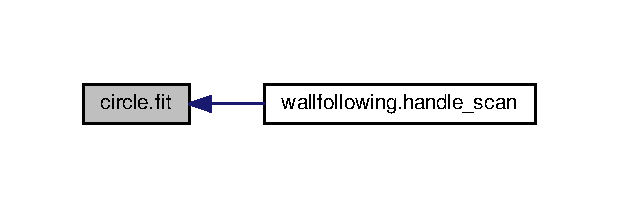
\includegraphics[width=297pt]{namespacecircle_a391c3f0ba3506996d7eb3384bf6eeca6_icgraph}
\end{center}
\end{figure}


\index{circle@{circle}!sigma@{sigma}}
\index{sigma@{sigma}!circle@{circle}}
\subsubsection[{\texorpdfstring{sigma(coords, x, y, r)}{sigma(coords, x, y, r)}}]{\setlength{\rightskip}{0pt plus 5cm}def circle.\+sigma (
\begin{DoxyParamCaption}
\item[{}]{coords, }
\item[{}]{x, }
\item[{}]{y, }
\item[{}]{r}
\end{DoxyParamCaption}
)}\hypertarget{namespacecircle_a35f5f3f41d4a120bf24f359fed22ab0d}{}\label{namespacecircle_a35f5f3f41d4a120bf24f359fed22ab0d}
\begin{DoxyVerb}Computes Sigma for circle fit.\end{DoxyVerb}
 

Definition at line 44 of file circle.\+py.



\subsection{Variable Documentation}
\index{circle@{circle}!Point@{Point}}
\index{Point@{Point}!circle@{circle}}
\subsubsection[{\texorpdfstring{Point}{Point}}]{\setlength{\rightskip}{0pt plus 5cm}circle.\+Point = namedtuple(\char`\"{}Point\char`\"{}, \mbox{[}\char`\"{}x\char`\"{}, \char`\"{}y\char`\"{}\mbox{]})}\hypertarget{namespacecircle_ae073d8de4a1ba7a4a4920f35128f1c48}{}\label{namespacecircle_ae073d8de4a1ba7a4a4920f35128f1c48}


Definition at line 9 of file circle.\+py.


\hypertarget{namespacedrive}{}\section{drive Namespace Reference}
\label{namespacedrive}\index{drive@{drive}}
\subsection*{Variables}
\begin{DoxyCompactItemize}
\item 
\hyperlink{namespacedrive_a417833a8f645f1b27a7285408616a9f0}{anonymous}
\item 
\hyperlink{namespacedrive_ad7f80b53042960cd3cf968dee1ebb197}{timer} = rospy.\+Rate(U\+P\+D\+A\+T\+E\+\_\+\+F\+R\+E\+Q\+U\+E\+N\+CY)
\item 
\hyperlink{namespacedrive_a23cc38e06b9fae695cf8845a82fcc273}{device} = torch.\+device(\char`\"{}cuda\char`\"{} if torch.\+cuda.\+is\+\_\+available() else \char`\"{}cpu\char`\"{})
\item 
\hyperlink{namespacedrive_a2e630ff72576502d513dc46034787985}{policy\+\_\+net} = \hyperlink{classparameters_1_1_neural_q_estimator}{Neural\+Q\+Estimator}().to(\hyperlink{namespacedrive_a23cc38e06b9fae695cf8845a82fcc273}{device})
\item 
string \hyperlink{namespacedrive_a82ba3ae0a4aeed9a874c1d9f87e147fd}{message} = \char`\"{}Model parameters for the neural net not found. You need to train it first.\char`\"{}
\item 
\hyperlink{namespacedrive_a082ee6b5d0f5566c851367e7c7792ea5}{scan} = \hyperlink{namespacecar_af96ea5ae50f968d7a2ff6bcc21cad1c2}{car.\+get\+\_\+scan}(L\+A\+S\+E\+R\+\_\+\+S\+A\+M\+P\+L\+E\+\_\+\+C\+O\+U\+NT, \hyperlink{namespacedrive_a23cc38e06b9fae695cf8845a82fcc273}{device})
\item 
\hyperlink{namespacedrive_aa0be36d022218be529fdf22d34a4dfc7}{net\+\_\+output} = \hyperlink{namespacedrive_a2e630ff72576502d513dc46034787985}{policy\+\_\+net}(\hyperlink{namespacedrive_a082ee6b5d0f5566c851367e7c7792ea5}{scan})
\item 
\hyperlink{namespacedrive_a63845082ab90bdcccd95631ad6420392}{action\+\_\+index} = net\+\_\+output.\+max(0)\mbox{[}1\mbox{]}.item()
\item 
\hyperlink{namespacedrive_a68b3f3acb667a1c5e05d3ea265164d7a}{action} = A\+C\+T\+I\+O\+NS\mbox{[}\hyperlink{namespacedrive_a63845082ab90bdcccd95631ad6420392}{action\+\_\+index}\mbox{]}
\end{DoxyCompactItemize}


\subsection{Variable Documentation}
\index{drive@{drive}!action@{action}}
\index{action@{action}!drive@{drive}}
\subsubsection[{\texorpdfstring{action}{action}}]{\setlength{\rightskip}{0pt plus 5cm}drive.\+action = A\+C\+T\+I\+O\+NS\mbox{[}{\bf action\+\_\+index}\mbox{]}}\hypertarget{namespacedrive_a68b3f3acb667a1c5e05d3ea265164d7a}{}\label{namespacedrive_a68b3f3acb667a1c5e05d3ea265164d7a}


Definition at line 28 of file drive.\+py.

\index{drive@{drive}!action\+\_\+index@{action\+\_\+index}}
\index{action\+\_\+index@{action\+\_\+index}!drive@{drive}}
\subsubsection[{\texorpdfstring{action\+\_\+index}{action_index}}]{\setlength{\rightskip}{0pt plus 5cm}drive.\+action\+\_\+index = net\+\_\+output.\+max(0)\mbox{[}1\mbox{]}.item()}\hypertarget{namespacedrive_a63845082ab90bdcccd95631ad6420392}{}\label{namespacedrive_a63845082ab90bdcccd95631ad6420392}


Definition at line 27 of file drive.\+py.

\index{drive@{drive}!anonymous@{anonymous}}
\index{anonymous@{anonymous}!drive@{drive}}
\subsubsection[{\texorpdfstring{anonymous}{anonymous}}]{\setlength{\rightskip}{0pt plus 5cm}drive.\+anonymous}\hypertarget{namespacedrive_a417833a8f645f1b27a7285408616a9f0}{}\label{namespacedrive_a417833a8f645f1b27a7285408616a9f0}


Definition at line 9 of file drive.\+py.

\index{drive@{drive}!device@{device}}
\index{device@{device}!drive@{drive}}
\subsubsection[{\texorpdfstring{device}{device}}]{\setlength{\rightskip}{0pt plus 5cm}drive.\+device = torch.\+device(\char`\"{}cuda\char`\"{} if torch.\+cuda.\+is\+\_\+available() else \char`\"{}cpu\char`\"{})}\hypertarget{namespacedrive_a23cc38e06b9fae695cf8845a82fcc273}{}\label{namespacedrive_a23cc38e06b9fae695cf8845a82fcc273}


Definition at line 13 of file drive.\+py.

\index{drive@{drive}!message@{message}}
\index{message@{message}!drive@{drive}}
\subsubsection[{\texorpdfstring{message}{message}}]{\setlength{\rightskip}{0pt plus 5cm}string drive.\+message = \char`\"{}Model parameters for the neural net not found. You need to train it first.\char`\"{}}\hypertarget{namespacedrive_a82ba3ae0a4aeed9a874c1d9f87e147fd}{}\label{namespacedrive_a82ba3ae0a4aeed9a874c1d9f87e147fd}


Definition at line 18 of file drive.\+py.

\index{drive@{drive}!net\+\_\+output@{net\+\_\+output}}
\index{net\+\_\+output@{net\+\_\+output}!drive@{drive}}
\subsubsection[{\texorpdfstring{net\+\_\+output}{net_output}}]{\setlength{\rightskip}{0pt plus 5cm}drive.\+net\+\_\+output = {\bf policy\+\_\+net}({\bf scan})}\hypertarget{namespacedrive_aa0be36d022218be529fdf22d34a4dfc7}{}\label{namespacedrive_aa0be36d022218be529fdf22d34a4dfc7}


Definition at line 26 of file drive.\+py.

\index{drive@{drive}!policy\+\_\+net@{policy\+\_\+net}}
\index{policy\+\_\+net@{policy\+\_\+net}!drive@{drive}}
\subsubsection[{\texorpdfstring{policy\+\_\+net}{policy_net}}]{\setlength{\rightskip}{0pt plus 5cm}drive.\+policy\+\_\+net = {\bf Neural\+Q\+Estimator}().to({\bf device})}\hypertarget{namespacedrive_a2e630ff72576502d513dc46034787985}{}\label{namespacedrive_a2e630ff72576502d513dc46034787985}


Definition at line 14 of file drive.\+py.

\index{drive@{drive}!scan@{scan}}
\index{scan@{scan}!drive@{drive}}
\subsubsection[{\texorpdfstring{scan}{scan}}]{\setlength{\rightskip}{0pt plus 5cm}drive.\+scan = {\bf car.\+get\+\_\+scan}(L\+A\+S\+E\+R\+\_\+\+S\+A\+M\+P\+L\+E\+\_\+\+C\+O\+U\+NT, {\bf device})}\hypertarget{namespacedrive_a082ee6b5d0f5566c851367e7c7792ea5}{}\label{namespacedrive_a082ee6b5d0f5566c851367e7c7792ea5}


Definition at line 24 of file drive.\+py.

\index{drive@{drive}!timer@{timer}}
\index{timer@{timer}!drive@{drive}}
\subsubsection[{\texorpdfstring{timer}{timer}}]{\setlength{\rightskip}{0pt plus 5cm}drive.\+timer = rospy.\+Rate(U\+P\+D\+A\+T\+E\+\_\+\+F\+R\+E\+Q\+U\+E\+N\+CY)}\hypertarget{namespacedrive_ad7f80b53042960cd3cf968dee1ebb197}{}\label{namespacedrive_ad7f80b53042960cd3cf968dee1ebb197}


Definition at line 11 of file drive.\+py.


\hypertarget{namespaceparameters}{}\section{parameters Namespace Reference}
\label{namespaceparameters}\index{parameters@{parameters}}
\subsection*{Classes}
\begin{DoxyCompactItemize}
\item 
class \hyperlink{classparameters_1_1_neural_q_estimator}{Neural\+Q\+Estimator}
\end{DoxyCompactItemize}
\subsection*{Variables}
\begin{DoxyCompactItemize}
\item 
string \hyperlink{namespaceparameters_a855cb11de60782b8e9997af80bdab518}{T\+O\+P\+I\+C\+\_\+\+D\+R\+I\+V\+E\+\_\+\+P\+A\+R\+A\+M\+E\+T\+E\+RS} = \char`\"{}/input/drive\+\_\+param/autonomous\char`\"{}
\item 
string \hyperlink{namespaceparameters_a28de242cdbba10666eb0c95aaef6812b}{T\+O\+P\+I\+C\+\_\+\+S\+C\+AN} = \char`\"{}/scan\char`\"{}
\item 
string \hyperlink{namespaceparameters_a5e392ed4d998f10824bfd96a0eae2988}{T\+O\+P\+I\+C\+\_\+\+C\+R\+A\+SH} = \char`\"{}/crash\char`\"{}
\item 
string \hyperlink{namespaceparameters_a9d4157266ec0afde91ab7d58be4f688d}{T\+O\+P\+I\+C\+\_\+\+G\+A\+Z\+E\+B\+O\+\_\+\+M\+O\+D\+E\+L\+\_\+\+S\+T\+A\+TE} = \char`\"{}/gazebo/model\+\_\+states\char`\"{}
\item 
string \hyperlink{namespaceparameters_aa69db8cd2d598f0d10212ea8df6a2139}{T\+O\+P\+I\+C\+\_\+\+E\+P\+I\+S\+O\+D\+E\+\_\+\+R\+E\+S\+U\+LT} = \char`\"{}/qlearning/episode\+\_\+result\char`\"{}
\item 
list \hyperlink{namespaceparameters_a585a25d0a26bcab4242d2e3fb1c1f93e}{A\+C\+T\+I\+O\+NS} = \mbox{[}(-\/0.\+6, 0.\+2), (0.\+6, 0.\+2), (0, 0.\+2)\mbox{]}
\item 
\hyperlink{namespaceparameters_ae4be13f6dac91f471da3efb4618a54c1}{A\+C\+T\+I\+O\+N\+\_\+\+C\+O\+U\+NT} = len(\hyperlink{namespaceparameters_a585a25d0a26bcab4242d2e3fb1c1f93e}{A\+C\+T\+I\+O\+NS})
\item 
int \hyperlink{namespaceparameters_a24735dce78cf9899cf1ec4bda2ea4eac}{L\+A\+S\+E\+R\+\_\+\+S\+A\+M\+P\+L\+E\+\_\+\+C\+O\+U\+NT} = 32
\item 
\hyperlink{namespaceparameters_aff8b0668384f3fa2d1212d3bd0ff42fa}{M\+O\+D\+E\+L\+\_\+\+F\+I\+L\+E\+N\+A\+ME} = os.\+path.\+join(Ros\+Pack().get\+\_\+path(\char`\"{}q\+\_\+learning\char`\"{}), \char`\"{}model.\+to\char`\"{})
\item 
bool \hyperlink{namespaceparameters_a0cffcb215ac12a1700baedb1a13ec8d5}{U\+S\+E\+\_\+\+E\+X\+I\+S\+T\+I\+N\+G\+\_\+\+P\+A\+R\+A\+M\+E\+T\+E\+RS} = False
\item 
float \hyperlink{namespaceparameters_a70176024e0f585c846365800f1c7819c}{D\+I\+S\+C\+O\+U\+N\+T\+\_\+\+F\+A\+C\+T\+OR} = 0.\+99
\item 
int \hyperlink{namespaceparameters_aa473cc3b100416af3310c6c5a6d19570}{M\+A\+X\+\_\+\+E\+P\+I\+S\+O\+D\+E\+\_\+\+L\+E\+N\+G\+TH} = 500
\item 
int \hyperlink{namespaceparameters_a49f1ad074b5710a98fc783c5627ddade}{M\+E\+M\+O\+R\+Y\+\_\+\+S\+I\+ZE} = 5000
\item 
int \hyperlink{namespaceparameters_a2d37d9950f7a887014021ab455282af6}{B\+A\+T\+C\+H\+\_\+\+S\+I\+ZE} = 128
\item 
float \hyperlink{namespaceparameters_afb996d542e8c3d3e8bbdfe4a711694dd}{L\+E\+A\+R\+N\+I\+N\+G\+\_\+\+R\+A\+TE} = 0.\+0001
\item 
float \hyperlink{namespaceparameters_a371d0de003e9046dcc72450b7512ce14}{E\+P\+S\+\_\+\+S\+T\+A\+RT} = 1.\+0
\item 
float \hyperlink{namespaceparameters_a3765f189d3af4815766ded3bffcba1e2}{E\+P\+S\+\_\+\+E\+ND} = 0.\+3
\item 
int \hyperlink{namespaceparameters_ab9a88c663385563b35331bbea5c4a74b}{E\+P\+S\+\_\+\+D\+E\+C\+AY} = 10000
\end{DoxyCompactItemize}


\subsection{Variable Documentation}
\index{parameters@{parameters}!A\+C\+T\+I\+O\+N\+\_\+\+C\+O\+U\+NT@{A\+C\+T\+I\+O\+N\+\_\+\+C\+O\+U\+NT}}
\index{A\+C\+T\+I\+O\+N\+\_\+\+C\+O\+U\+NT@{A\+C\+T\+I\+O\+N\+\_\+\+C\+O\+U\+NT}!parameters@{parameters}}
\subsubsection[{\texorpdfstring{A\+C\+T\+I\+O\+N\+\_\+\+C\+O\+U\+NT}{ACTION_COUNT}}]{\setlength{\rightskip}{0pt plus 5cm}parameters.\+A\+C\+T\+I\+O\+N\+\_\+\+C\+O\+U\+NT = len({\bf A\+C\+T\+I\+O\+NS})}\hypertarget{namespaceparameters_ae4be13f6dac91f471da3efb4618a54c1}{}\label{namespaceparameters_ae4be13f6dac91f471da3efb4618a54c1}


Definition at line 20 of file parameters.\+py.

\index{parameters@{parameters}!A\+C\+T\+I\+O\+NS@{A\+C\+T\+I\+O\+NS}}
\index{A\+C\+T\+I\+O\+NS@{A\+C\+T\+I\+O\+NS}!parameters@{parameters}}
\subsubsection[{\texorpdfstring{A\+C\+T\+I\+O\+NS}{ACTIONS}}]{\setlength{\rightskip}{0pt plus 5cm}list parameters.\+A\+C\+T\+I\+O\+NS = \mbox{[}(-\/0.\+6, 0.\+2), (0.\+6, 0.\+2), (0, 0.\+2)\mbox{]}}\hypertarget{namespaceparameters_a585a25d0a26bcab4242d2e3fb1c1f93e}{}\label{namespaceparameters_a585a25d0a26bcab4242d2e3fb1c1f93e}


Definition at line 19 of file parameters.\+py.

\index{parameters@{parameters}!B\+A\+T\+C\+H\+\_\+\+S\+I\+ZE@{B\+A\+T\+C\+H\+\_\+\+S\+I\+ZE}}
\index{B\+A\+T\+C\+H\+\_\+\+S\+I\+ZE@{B\+A\+T\+C\+H\+\_\+\+S\+I\+ZE}!parameters@{parameters}}
\subsubsection[{\texorpdfstring{B\+A\+T\+C\+H\+\_\+\+S\+I\+ZE}{BATCH_SIZE}}]{\setlength{\rightskip}{0pt plus 5cm}int parameters.\+B\+A\+T\+C\+H\+\_\+\+S\+I\+ZE = 128}\hypertarget{namespaceparameters_a2d37d9950f7a887014021ab455282af6}{}\label{namespaceparameters_a2d37d9950f7a887014021ab455282af6}


Definition at line 63 of file parameters.\+py.

\index{parameters@{parameters}!D\+I\+S\+C\+O\+U\+N\+T\+\_\+\+F\+A\+C\+T\+OR@{D\+I\+S\+C\+O\+U\+N\+T\+\_\+\+F\+A\+C\+T\+OR}}
\index{D\+I\+S\+C\+O\+U\+N\+T\+\_\+\+F\+A\+C\+T\+OR@{D\+I\+S\+C\+O\+U\+N\+T\+\_\+\+F\+A\+C\+T\+OR}!parameters@{parameters}}
\subsubsection[{\texorpdfstring{D\+I\+S\+C\+O\+U\+N\+T\+\_\+\+F\+A\+C\+T\+OR}{DISCOUNT_FACTOR}}]{\setlength{\rightskip}{0pt plus 5cm}float parameters.\+D\+I\+S\+C\+O\+U\+N\+T\+\_\+\+F\+A\+C\+T\+OR = 0.\+99}\hypertarget{namespaceparameters_a70176024e0f585c846365800f1c7819c}{}\label{namespaceparameters_a70176024e0f585c846365800f1c7819c}


Definition at line 56 of file parameters.\+py.

\index{parameters@{parameters}!E\+P\+S\+\_\+\+D\+E\+C\+AY@{E\+P\+S\+\_\+\+D\+E\+C\+AY}}
\index{E\+P\+S\+\_\+\+D\+E\+C\+AY@{E\+P\+S\+\_\+\+D\+E\+C\+AY}!parameters@{parameters}}
\subsubsection[{\texorpdfstring{E\+P\+S\+\_\+\+D\+E\+C\+AY}{EPS_DECAY}}]{\setlength{\rightskip}{0pt plus 5cm}int parameters.\+E\+P\+S\+\_\+\+D\+E\+C\+AY = 10000}\hypertarget{namespaceparameters_ab9a88c663385563b35331bbea5c4a74b}{}\label{namespaceparameters_ab9a88c663385563b35331bbea5c4a74b}


Definition at line 70 of file parameters.\+py.

\index{parameters@{parameters}!E\+P\+S\+\_\+\+E\+ND@{E\+P\+S\+\_\+\+E\+ND}}
\index{E\+P\+S\+\_\+\+E\+ND@{E\+P\+S\+\_\+\+E\+ND}!parameters@{parameters}}
\subsubsection[{\texorpdfstring{E\+P\+S\+\_\+\+E\+ND}{EPS_END}}]{\setlength{\rightskip}{0pt plus 5cm}float parameters.\+E\+P\+S\+\_\+\+E\+ND = 0.\+3}\hypertarget{namespaceparameters_a3765f189d3af4815766ded3bffcba1e2}{}\label{namespaceparameters_a3765f189d3af4815766ded3bffcba1e2}


Definition at line 69 of file parameters.\+py.

\index{parameters@{parameters}!E\+P\+S\+\_\+\+S\+T\+A\+RT@{E\+P\+S\+\_\+\+S\+T\+A\+RT}}
\index{E\+P\+S\+\_\+\+S\+T\+A\+RT@{E\+P\+S\+\_\+\+S\+T\+A\+RT}!parameters@{parameters}}
\subsubsection[{\texorpdfstring{E\+P\+S\+\_\+\+S\+T\+A\+RT}{EPS_START}}]{\setlength{\rightskip}{0pt plus 5cm}float parameters.\+E\+P\+S\+\_\+\+S\+T\+A\+RT = 1.\+0}\hypertarget{namespaceparameters_a371d0de003e9046dcc72450b7512ce14}{}\label{namespaceparameters_a371d0de003e9046dcc72450b7512ce14}


Definition at line 68 of file parameters.\+py.

\index{parameters@{parameters}!L\+A\+S\+E\+R\+\_\+\+S\+A\+M\+P\+L\+E\+\_\+\+C\+O\+U\+NT@{L\+A\+S\+E\+R\+\_\+\+S\+A\+M\+P\+L\+E\+\_\+\+C\+O\+U\+NT}}
\index{L\+A\+S\+E\+R\+\_\+\+S\+A\+M\+P\+L\+E\+\_\+\+C\+O\+U\+NT@{L\+A\+S\+E\+R\+\_\+\+S\+A\+M\+P\+L\+E\+\_\+\+C\+O\+U\+NT}!parameters@{parameters}}
\subsubsection[{\texorpdfstring{L\+A\+S\+E\+R\+\_\+\+S\+A\+M\+P\+L\+E\+\_\+\+C\+O\+U\+NT}{LASER_SAMPLE_COUNT}}]{\setlength{\rightskip}{0pt plus 5cm}int parameters.\+L\+A\+S\+E\+R\+\_\+\+S\+A\+M\+P\+L\+E\+\_\+\+C\+O\+U\+NT = 32}\hypertarget{namespaceparameters_a24735dce78cf9899cf1ec4bda2ea4eac}{}\label{namespaceparameters_a24735dce78cf9899cf1ec4bda2ea4eac}


Definition at line 24 of file parameters.\+py.

\index{parameters@{parameters}!L\+E\+A\+R\+N\+I\+N\+G\+\_\+\+R\+A\+TE@{L\+E\+A\+R\+N\+I\+N\+G\+\_\+\+R\+A\+TE}}
\index{L\+E\+A\+R\+N\+I\+N\+G\+\_\+\+R\+A\+TE@{L\+E\+A\+R\+N\+I\+N\+G\+\_\+\+R\+A\+TE}!parameters@{parameters}}
\subsubsection[{\texorpdfstring{L\+E\+A\+R\+N\+I\+N\+G\+\_\+\+R\+A\+TE}{LEARNING_RATE}}]{\setlength{\rightskip}{0pt plus 5cm}float parameters.\+L\+E\+A\+R\+N\+I\+N\+G\+\_\+\+R\+A\+TE = 0.\+0001}\hypertarget{namespaceparameters_afb996d542e8c3d3e8bbdfe4a711694dd}{}\label{namespaceparameters_afb996d542e8c3d3e8bbdfe4a711694dd}


Definition at line 64 of file parameters.\+py.

\index{parameters@{parameters}!M\+A\+X\+\_\+\+E\+P\+I\+S\+O\+D\+E\+\_\+\+L\+E\+N\+G\+TH@{M\+A\+X\+\_\+\+E\+P\+I\+S\+O\+D\+E\+\_\+\+L\+E\+N\+G\+TH}}
\index{M\+A\+X\+\_\+\+E\+P\+I\+S\+O\+D\+E\+\_\+\+L\+E\+N\+G\+TH@{M\+A\+X\+\_\+\+E\+P\+I\+S\+O\+D\+E\+\_\+\+L\+E\+N\+G\+TH}!parameters@{parameters}}
\subsubsection[{\texorpdfstring{M\+A\+X\+\_\+\+E\+P\+I\+S\+O\+D\+E\+\_\+\+L\+E\+N\+G\+TH}{MAX_EPISODE_LENGTH}}]{\setlength{\rightskip}{0pt plus 5cm}int parameters.\+M\+A\+X\+\_\+\+E\+P\+I\+S\+O\+D\+E\+\_\+\+L\+E\+N\+G\+TH = 500}\hypertarget{namespaceparameters_aa473cc3b100416af3310c6c5a6d19570}{}\label{namespaceparameters_aa473cc3b100416af3310c6c5a6d19570}


Definition at line 58 of file parameters.\+py.

\index{parameters@{parameters}!M\+E\+M\+O\+R\+Y\+\_\+\+S\+I\+ZE@{M\+E\+M\+O\+R\+Y\+\_\+\+S\+I\+ZE}}
\index{M\+E\+M\+O\+R\+Y\+\_\+\+S\+I\+ZE@{M\+E\+M\+O\+R\+Y\+\_\+\+S\+I\+ZE}!parameters@{parameters}}
\subsubsection[{\texorpdfstring{M\+E\+M\+O\+R\+Y\+\_\+\+S\+I\+ZE}{MEMORY_SIZE}}]{\setlength{\rightskip}{0pt plus 5cm}int parameters.\+M\+E\+M\+O\+R\+Y\+\_\+\+S\+I\+ZE = 5000}\hypertarget{namespaceparameters_a49f1ad074b5710a98fc783c5627ddade}{}\label{namespaceparameters_a49f1ad074b5710a98fc783c5627ddade}


Definition at line 61 of file parameters.\+py.

\index{parameters@{parameters}!M\+O\+D\+E\+L\+\_\+\+F\+I\+L\+E\+N\+A\+ME@{M\+O\+D\+E\+L\+\_\+\+F\+I\+L\+E\+N\+A\+ME}}
\index{M\+O\+D\+E\+L\+\_\+\+F\+I\+L\+E\+N\+A\+ME@{M\+O\+D\+E\+L\+\_\+\+F\+I\+L\+E\+N\+A\+ME}!parameters@{parameters}}
\subsubsection[{\texorpdfstring{M\+O\+D\+E\+L\+\_\+\+F\+I\+L\+E\+N\+A\+ME}{MODEL_FILENAME}}]{\setlength{\rightskip}{0pt plus 5cm}parameters.\+M\+O\+D\+E\+L\+\_\+\+F\+I\+L\+E\+N\+A\+ME = os.\+path.\+join(Ros\+Pack().get\+\_\+path(\char`\"{}q\+\_\+learning\char`\"{}), \char`\"{}model.\+to\char`\"{})}\hypertarget{namespaceparameters_aff8b0668384f3fa2d1212d3bd0ff42fa}{}\label{namespaceparameters_aff8b0668384f3fa2d1212d3bd0ff42fa}


Definition at line 27 of file parameters.\+py.

\index{parameters@{parameters}!T\+O\+P\+I\+C\+\_\+\+C\+R\+A\+SH@{T\+O\+P\+I\+C\+\_\+\+C\+R\+A\+SH}}
\index{T\+O\+P\+I\+C\+\_\+\+C\+R\+A\+SH@{T\+O\+P\+I\+C\+\_\+\+C\+R\+A\+SH}!parameters@{parameters}}
\subsubsection[{\texorpdfstring{T\+O\+P\+I\+C\+\_\+\+C\+R\+A\+SH}{TOPIC_CRASH}}]{\setlength{\rightskip}{0pt plus 5cm}string parameters.\+T\+O\+P\+I\+C\+\_\+\+C\+R\+A\+SH = \char`\"{}/crash\char`\"{}}\hypertarget{namespaceparameters_a5e392ed4d998f10824bfd96a0eae2988}{}\label{namespaceparameters_a5e392ed4d998f10824bfd96a0eae2988}


Definition at line 13 of file parameters.\+py.

\index{parameters@{parameters}!T\+O\+P\+I\+C\+\_\+\+D\+R\+I\+V\+E\+\_\+\+P\+A\+R\+A\+M\+E\+T\+E\+RS@{T\+O\+P\+I\+C\+\_\+\+D\+R\+I\+V\+E\+\_\+\+P\+A\+R\+A\+M\+E\+T\+E\+RS}}
\index{T\+O\+P\+I\+C\+\_\+\+D\+R\+I\+V\+E\+\_\+\+P\+A\+R\+A\+M\+E\+T\+E\+RS@{T\+O\+P\+I\+C\+\_\+\+D\+R\+I\+V\+E\+\_\+\+P\+A\+R\+A\+M\+E\+T\+E\+RS}!parameters@{parameters}}
\subsubsection[{\texorpdfstring{T\+O\+P\+I\+C\+\_\+\+D\+R\+I\+V\+E\+\_\+\+P\+A\+R\+A\+M\+E\+T\+E\+RS}{TOPIC_DRIVE_PARAMETERS}}]{\setlength{\rightskip}{0pt plus 5cm}string parameters.\+T\+O\+P\+I\+C\+\_\+\+D\+R\+I\+V\+E\+\_\+\+P\+A\+R\+A\+M\+E\+T\+E\+RS = \char`\"{}/input/drive\+\_\+param/autonomous\char`\"{}}\hypertarget{namespaceparameters_a855cb11de60782b8e9997af80bdab518}{}\label{namespaceparameters_a855cb11de60782b8e9997af80bdab518}


Definition at line 11 of file parameters.\+py.

\index{parameters@{parameters}!T\+O\+P\+I\+C\+\_\+\+E\+P\+I\+S\+O\+D\+E\+\_\+\+R\+E\+S\+U\+LT@{T\+O\+P\+I\+C\+\_\+\+E\+P\+I\+S\+O\+D\+E\+\_\+\+R\+E\+S\+U\+LT}}
\index{T\+O\+P\+I\+C\+\_\+\+E\+P\+I\+S\+O\+D\+E\+\_\+\+R\+E\+S\+U\+LT@{T\+O\+P\+I\+C\+\_\+\+E\+P\+I\+S\+O\+D\+E\+\_\+\+R\+E\+S\+U\+LT}!parameters@{parameters}}
\subsubsection[{\texorpdfstring{T\+O\+P\+I\+C\+\_\+\+E\+P\+I\+S\+O\+D\+E\+\_\+\+R\+E\+S\+U\+LT}{TOPIC_EPISODE_RESULT}}]{\setlength{\rightskip}{0pt plus 5cm}string parameters.\+T\+O\+P\+I\+C\+\_\+\+E\+P\+I\+S\+O\+D\+E\+\_\+\+R\+E\+S\+U\+LT = \char`\"{}/qlearning/episode\+\_\+result\char`\"{}}\hypertarget{namespaceparameters_aa69db8cd2d598f0d10212ea8df6a2139}{}\label{namespaceparameters_aa69db8cd2d598f0d10212ea8df6a2139}


Definition at line 15 of file parameters.\+py.

\index{parameters@{parameters}!T\+O\+P\+I\+C\+\_\+\+G\+A\+Z\+E\+B\+O\+\_\+\+M\+O\+D\+E\+L\+\_\+\+S\+T\+A\+TE@{T\+O\+P\+I\+C\+\_\+\+G\+A\+Z\+E\+B\+O\+\_\+\+M\+O\+D\+E\+L\+\_\+\+S\+T\+A\+TE}}
\index{T\+O\+P\+I\+C\+\_\+\+G\+A\+Z\+E\+B\+O\+\_\+\+M\+O\+D\+E\+L\+\_\+\+S\+T\+A\+TE@{T\+O\+P\+I\+C\+\_\+\+G\+A\+Z\+E\+B\+O\+\_\+\+M\+O\+D\+E\+L\+\_\+\+S\+T\+A\+TE}!parameters@{parameters}}
\subsubsection[{\texorpdfstring{T\+O\+P\+I\+C\+\_\+\+G\+A\+Z\+E\+B\+O\+\_\+\+M\+O\+D\+E\+L\+\_\+\+S\+T\+A\+TE}{TOPIC_GAZEBO_MODEL_STATE}}]{\setlength{\rightskip}{0pt plus 5cm}string parameters.\+T\+O\+P\+I\+C\+\_\+\+G\+A\+Z\+E\+B\+O\+\_\+\+M\+O\+D\+E\+L\+\_\+\+S\+T\+A\+TE = \char`\"{}/gazebo/model\+\_\+states\char`\"{}}\hypertarget{namespaceparameters_a9d4157266ec0afde91ab7d58be4f688d}{}\label{namespaceparameters_a9d4157266ec0afde91ab7d58be4f688d}


Definition at line 14 of file parameters.\+py.

\index{parameters@{parameters}!T\+O\+P\+I\+C\+\_\+\+S\+C\+AN@{T\+O\+P\+I\+C\+\_\+\+S\+C\+AN}}
\index{T\+O\+P\+I\+C\+\_\+\+S\+C\+AN@{T\+O\+P\+I\+C\+\_\+\+S\+C\+AN}!parameters@{parameters}}
\subsubsection[{\texorpdfstring{T\+O\+P\+I\+C\+\_\+\+S\+C\+AN}{TOPIC_SCAN}}]{\setlength{\rightskip}{0pt plus 5cm}string parameters.\+T\+O\+P\+I\+C\+\_\+\+S\+C\+AN = \char`\"{}/scan\char`\"{}}\hypertarget{namespaceparameters_a28de242cdbba10666eb0c95aaef6812b}{}\label{namespaceparameters_a28de242cdbba10666eb0c95aaef6812b}


Definition at line 12 of file parameters.\+py.

\index{parameters@{parameters}!U\+S\+E\+\_\+\+E\+X\+I\+S\+T\+I\+N\+G\+\_\+\+P\+A\+R\+A\+M\+E\+T\+E\+RS@{U\+S\+E\+\_\+\+E\+X\+I\+S\+T\+I\+N\+G\+\_\+\+P\+A\+R\+A\+M\+E\+T\+E\+RS}}
\index{U\+S\+E\+\_\+\+E\+X\+I\+S\+T\+I\+N\+G\+\_\+\+P\+A\+R\+A\+M\+E\+T\+E\+RS@{U\+S\+E\+\_\+\+E\+X\+I\+S\+T\+I\+N\+G\+\_\+\+P\+A\+R\+A\+M\+E\+T\+E\+RS}!parameters@{parameters}}
\subsubsection[{\texorpdfstring{U\+S\+E\+\_\+\+E\+X\+I\+S\+T\+I\+N\+G\+\_\+\+P\+A\+R\+A\+M\+E\+T\+E\+RS}{USE_EXISTING_PARAMETERS}}]{\setlength{\rightskip}{0pt plus 5cm}bool parameters.\+U\+S\+E\+\_\+\+E\+X\+I\+S\+T\+I\+N\+G\+\_\+\+P\+A\+R\+A\+M\+E\+T\+E\+RS = False}\hypertarget{namespaceparameters_a0cffcb215ac12a1700baedb1a13ec8d5}{}\label{namespaceparameters_a0cffcb215ac12a1700baedb1a13ec8d5}


Definition at line 54 of file parameters.\+py.


\hypertarget{namespaceplotter}{}\section{plotter Namespace Reference}
\label{namespaceplotter}\index{plotter@{plotter}}
\subsection*{Functions}
\begin{DoxyCompactItemize}
\item 
def \hyperlink{namespaceplotter_a4dd8967dd22ff14b03fcc921ec7dcc3d}{update\+\_\+plot} (msg)
\end{DoxyCompactItemize}
\subsection*{Variables}
\begin{DoxyCompactItemize}
\item 
\hyperlink{namespaceplotter_abbb49ab9c0174321374123fd800937f1}{plot\+\_\+window} = rospy.\+get\+\_\+param(\char`\"{}$\sim$plot\+\_\+window\char`\"{})
\item 
\hyperlink{namespaceplotter_aa648ebbb57476267f9430be51eeb420c}{reward\+\_\+list} = deque(maxlen=\hyperlink{namespaceplotter_abbb49ab9c0174321374123fd800937f1}{plot\+\_\+window})
\item 
\hyperlink{namespaceplotter_ab7eba5fc23c3791ab6bca7c5c975d2b8}{length\+\_\+list} = deque(maxlen=\hyperlink{namespaceplotter_abbb49ab9c0174321374123fd800937f1}{plot\+\_\+window})
\item 
int \hyperlink{namespaceplotter_aec1d6d729c0b25355f045e1f5bdc588f}{episode\+\_\+count} = 0
\item 
\hyperlink{namespaceplotter_ab20bf5077ebe79698f5f02f62dcb33d2}{app} = Qt\+Gui.\+Q\+Application(sys.\+argv)
\item 
\hyperlink{namespaceplotter_aac09effafbbcb0f637092be85f99c351}{app\+\_\+window} = pg.\+Graphics\+Window(title=\textquotesingle{}Learning Progress\textquotesingle{})
\item 
\hyperlink{namespaceplotter_a40d656a97d2e7039f17ee5742490ecf9}{main\+\_\+plot} = app\+\_\+window.\+add\+Plot(title=\textquotesingle{}Episodes\textquotesingle{})
\item 
\hyperlink{namespaceplotter_ac0842708a1e94becc6bb776a68a9ac5f}{length\+\_\+plot} = main\+\_\+plot.\+plot(pen=\textquotesingle{}g\textquotesingle{}, name=\textquotesingle{}length\textquotesingle{})
\item 
\hyperlink{namespaceplotter_a40062593c153ab9d59f836890f82dfc7}{reward\+\_\+plot} = main\+\_\+plot.\+plot(pen=\textquotesingle{}r\textquotesingle{}, name=\textquotesingle{}reward\textquotesingle{})
\end{DoxyCompactItemize}


\subsection{Function Documentation}
\index{plotter@{plotter}!update\+\_\+plot@{update\+\_\+plot}}
\index{update\+\_\+plot@{update\+\_\+plot}!plotter@{plotter}}
\subsubsection[{\texorpdfstring{update\+\_\+plot(msg)}{update_plot(msg)}}]{\setlength{\rightskip}{0pt plus 5cm}def plotter.\+update\+\_\+plot (
\begin{DoxyParamCaption}
\item[{}]{msg}
\end{DoxyParamCaption}
)}\hypertarget{namespaceplotter_a4dd8967dd22ff14b03fcc921ec7dcc3d}{}\label{namespaceplotter_a4dd8967dd22ff14b03fcc921ec7dcc3d}


Definition at line 12 of file plotter.\+py.



\subsection{Variable Documentation}
\index{plotter@{plotter}!app@{app}}
\index{app@{app}!plotter@{plotter}}
\subsubsection[{\texorpdfstring{app}{app}}]{\setlength{\rightskip}{0pt plus 5cm}plotter.\+app = Qt\+Gui.\+Q\+Application(sys.\+argv)}\hypertarget{namespaceplotter_ab20bf5077ebe79698f5f02f62dcb33d2}{}\label{namespaceplotter_ab20bf5077ebe79698f5f02f62dcb33d2}


Definition at line 31 of file plotter.\+py.

\index{plotter@{plotter}!app\+\_\+window@{app\+\_\+window}}
\index{app\+\_\+window@{app\+\_\+window}!plotter@{plotter}}
\subsubsection[{\texorpdfstring{app\+\_\+window}{app_window}}]{\setlength{\rightskip}{0pt plus 5cm}plotter.\+app\+\_\+window = pg.\+Graphics\+Window(title=\textquotesingle{}Learning Progress\textquotesingle{})}\hypertarget{namespaceplotter_aac09effafbbcb0f637092be85f99c351}{}\label{namespaceplotter_aac09effafbbcb0f637092be85f99c351}


Definition at line 32 of file plotter.\+py.

\index{plotter@{plotter}!episode\+\_\+count@{episode\+\_\+count}}
\index{episode\+\_\+count@{episode\+\_\+count}!plotter@{plotter}}
\subsubsection[{\texorpdfstring{episode\+\_\+count}{episode_count}}]{\setlength{\rightskip}{0pt plus 5cm}int plotter.\+episode\+\_\+count = 0}\hypertarget{namespaceplotter_aec1d6d729c0b25355f045e1f5bdc588f}{}\label{namespaceplotter_aec1d6d729c0b25355f045e1f5bdc588f}


Definition at line 29 of file plotter.\+py.

\index{plotter@{plotter}!length\+\_\+list@{length\+\_\+list}}
\index{length\+\_\+list@{length\+\_\+list}!plotter@{plotter}}
\subsubsection[{\texorpdfstring{length\+\_\+list}{length_list}}]{\setlength{\rightskip}{0pt plus 5cm}plotter.\+length\+\_\+list = deque(maxlen={\bf plot\+\_\+window})}\hypertarget{namespaceplotter_ab7eba5fc23c3791ab6bca7c5c975d2b8}{}\label{namespaceplotter_ab7eba5fc23c3791ab6bca7c5c975d2b8}


Definition at line 28 of file plotter.\+py.

\index{plotter@{plotter}!length\+\_\+plot@{length\+\_\+plot}}
\index{length\+\_\+plot@{length\+\_\+plot}!plotter@{plotter}}
\subsubsection[{\texorpdfstring{length\+\_\+plot}{length_plot}}]{\setlength{\rightskip}{0pt plus 5cm}plotter.\+length\+\_\+plot = main\+\_\+plot.\+plot(pen=\textquotesingle{}g\textquotesingle{}, name=\textquotesingle{}length\textquotesingle{})}\hypertarget{namespaceplotter_ac0842708a1e94becc6bb776a68a9ac5f}{}\label{namespaceplotter_ac0842708a1e94becc6bb776a68a9ac5f}


Definition at line 37 of file plotter.\+py.

\index{plotter@{plotter}!main\+\_\+plot@{main\+\_\+plot}}
\index{main\+\_\+plot@{main\+\_\+plot}!plotter@{plotter}}
\subsubsection[{\texorpdfstring{main\+\_\+plot}{main_plot}}]{\setlength{\rightskip}{0pt plus 5cm}plotter.\+main\+\_\+plot = app\+\_\+window.\+add\+Plot(title=\textquotesingle{}Episodes\textquotesingle{})}\hypertarget{namespaceplotter_a40d656a97d2e7039f17ee5742490ecf9}{}\label{namespaceplotter_a40d656a97d2e7039f17ee5742490ecf9}


Definition at line 33 of file plotter.\+py.

\index{plotter@{plotter}!plot\+\_\+window@{plot\+\_\+window}}
\index{plot\+\_\+window@{plot\+\_\+window}!plotter@{plotter}}
\subsubsection[{\texorpdfstring{plot\+\_\+window}{plot_window}}]{\setlength{\rightskip}{0pt plus 5cm}plotter.\+plot\+\_\+window = rospy.\+get\+\_\+param(\char`\"{}$\sim$plot\+\_\+window\char`\"{})}\hypertarget{namespaceplotter_abbb49ab9c0174321374123fd800937f1}{}\label{namespaceplotter_abbb49ab9c0174321374123fd800937f1}


Definition at line 25 of file plotter.\+py.

\index{plotter@{plotter}!reward\+\_\+list@{reward\+\_\+list}}
\index{reward\+\_\+list@{reward\+\_\+list}!plotter@{plotter}}
\subsubsection[{\texorpdfstring{reward\+\_\+list}{reward_list}}]{\setlength{\rightskip}{0pt plus 5cm}plotter.\+reward\+\_\+list = deque(maxlen={\bf plot\+\_\+window})}\hypertarget{namespaceplotter_aa648ebbb57476267f9430be51eeb420c}{}\label{namespaceplotter_aa648ebbb57476267f9430be51eeb420c}


Definition at line 27 of file plotter.\+py.

\index{plotter@{plotter}!reward\+\_\+plot@{reward\+\_\+plot}}
\index{reward\+\_\+plot@{reward\+\_\+plot}!plotter@{plotter}}
\subsubsection[{\texorpdfstring{reward\+\_\+plot}{reward_plot}}]{\setlength{\rightskip}{0pt plus 5cm}plotter.\+reward\+\_\+plot = main\+\_\+plot.\+plot(pen=\textquotesingle{}r\textquotesingle{}, name=\textquotesingle{}reward\textquotesingle{})}\hypertarget{namespaceplotter_a40062593c153ab9d59f836890f82dfc7}{}\label{namespaceplotter_a40062593c153ab9d59f836890f82dfc7}


Definition at line 38 of file plotter.\+py.


\hypertarget{namespaceqlearning}{}\section{qlearning Namespace Reference}
\label{namespaceqlearning}\index{qlearning@{qlearning}}
\subsection*{Classes}
\begin{DoxyCompactItemize}
\item 
class \hyperlink{classqlearning_1_1_q_learning_node}{Q\+Learning\+Node}
\end{DoxyCompactItemize}
\subsection*{Variables}
\begin{DoxyCompactItemize}
\item 
\hyperlink{namespaceqlearning_a6034910e71ae6db3114fb7b830d3e45d}{device} = torch.\+device(\char`\"{}cuda\char`\"{} if torch.\+cuda.\+is\+\_\+available() else \char`\"{}cpu\char`\"{})
\end{DoxyCompactItemize}


\subsection{Variable Documentation}
\index{qlearning@{qlearning}!device@{device}}
\index{device@{device}!qlearning@{qlearning}}
\subsubsection[{\texorpdfstring{device}{device}}]{\setlength{\rightskip}{0pt plus 5cm}qlearning.\+device = torch.\+device(\char`\"{}cuda\char`\"{} if torch.\+cuda.\+is\+\_\+available() else \char`\"{}cpu\char`\"{})}\hypertarget{namespaceqlearning_a6034910e71ae6db3114fb7b830d3e45d}{}\label{namespaceqlearning_a6034910e71ae6db3114fb7b830d3e45d}


Definition at line 48 of file qlearning.\+py.


\hypertarget{namespacerviz__geometry}{}\section{rviz\+\_\+geometry Namespace Reference}
\label{namespacerviz__geometry}\index{rviz\+\_\+geometry@{rviz\+\_\+geometry}}
\subsection*{Functions}
\begin{DoxyCompactItemize}
\item 
def \hyperlink{namespacerviz__geometry_a93390c23bebf8db38c31f832225dddda}{show\+\_\+line\+\_\+in\+\_\+rviz} (id, points, color, line\+\_\+width=0.\+02)
\item 
def \hyperlink{namespacerviz__geometry_a07a18d3bf4954414457db93c65b71c2e}{show\+\_\+circle\+\_\+in\+\_\+rviz} (circle, wall, id)
\end{DoxyCompactItemize}
\subsection*{Variables}
\begin{DoxyCompactItemize}
\item 
string \hyperlink{namespacerviz__geometry_a2bfe028bdabf1321495ece3cfc6b4fa6}{R\+V\+I\+Z\+\_\+\+T\+O\+P\+IC} = \char`\"{}/wallfollowing\+\_\+visualization\char`\"{}
\item 
string \hyperlink{namespacerviz__geometry_a3a3837887cc012683c1d87e5027b6863}{R\+V\+I\+Z\+\_\+\+F\+R\+A\+ME} = \char`\"{}laser\char`\"{}
\item 
string \hyperlink{namespacerviz__geometry_ad8626a9cfbc948e43f401fb1f3d62ecb}{R\+V\+I\+Z\+\_\+\+N\+A\+M\+E\+S\+P\+A\+CE} = \char`\"{}wall\+\_\+following\char`\"{}
\item 
\hyperlink{namespacerviz__geometry_ac4b20d63343627f7ac14151eba108ba8}{marker\+\_\+publisher} = rospy.\+Publisher(\hyperlink{namespacerviz__geometry_a2bfe028bdabf1321495ece3cfc6b4fa6}{R\+V\+I\+Z\+\_\+\+T\+O\+P\+IC}, Marker, queue\+\_\+size=1)
\end{DoxyCompactItemize}


\subsection{Function Documentation}
\index{rviz\+\_\+geometry@{rviz\+\_\+geometry}!show\+\_\+circle\+\_\+in\+\_\+rviz@{show\+\_\+circle\+\_\+in\+\_\+rviz}}
\index{show\+\_\+circle\+\_\+in\+\_\+rviz@{show\+\_\+circle\+\_\+in\+\_\+rviz}!rviz\+\_\+geometry@{rviz\+\_\+geometry}}
\subsubsection[{\texorpdfstring{show\+\_\+circle\+\_\+in\+\_\+rviz(circle, wall, id)}{show_circle_in_rviz(circle, wall, id)}}]{\setlength{\rightskip}{0pt plus 5cm}def rviz\+\_\+geometry.\+show\+\_\+circle\+\_\+in\+\_\+rviz (
\begin{DoxyParamCaption}
\item[{}]{circle, }
\item[{}]{wall, }
\item[{}]{id}
\end{DoxyParamCaption}
)}\hypertarget{namespacerviz__geometry_a07a18d3bf4954414457db93c65b71c2e}{}\label{namespacerviz__geometry_a07a18d3bf4954414457db93c65b71c2e}


Definition at line 38 of file rviz\+\_\+geometry.\+py.



Here is the call graph for this function\+:
\nopagebreak
\begin{figure}[H]
\begin{center}
\leavevmode
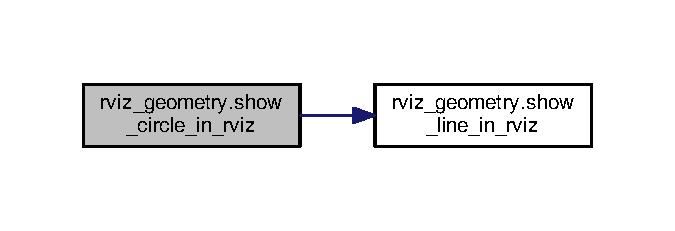
\includegraphics[width=324pt]{namespacerviz__geometry_a07a18d3bf4954414457db93c65b71c2e_cgraph}
\end{center}
\end{figure}




Here is the caller graph for this function\+:
\nopagebreak
\begin{figure}[H]
\begin{center}
\leavevmode
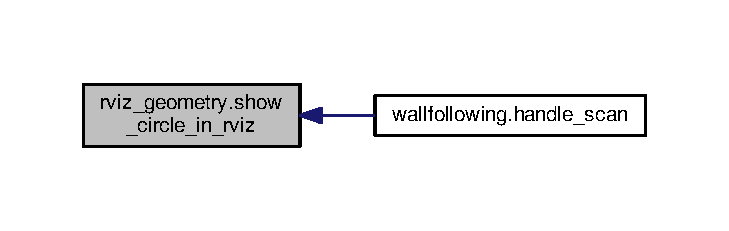
\includegraphics[width=350pt]{namespacerviz__geometry_a07a18d3bf4954414457db93c65b71c2e_icgraph}
\end{center}
\end{figure}


\index{rviz\+\_\+geometry@{rviz\+\_\+geometry}!show\+\_\+line\+\_\+in\+\_\+rviz@{show\+\_\+line\+\_\+in\+\_\+rviz}}
\index{show\+\_\+line\+\_\+in\+\_\+rviz@{show\+\_\+line\+\_\+in\+\_\+rviz}!rviz\+\_\+geometry@{rviz\+\_\+geometry}}
\subsubsection[{\texorpdfstring{show\+\_\+line\+\_\+in\+\_\+rviz(id, points, color, line\+\_\+width=0.\+02)}{show_line_in_rviz(id, points, color, line_width=0.02)}}]{\setlength{\rightskip}{0pt plus 5cm}def rviz\+\_\+geometry.\+show\+\_\+line\+\_\+in\+\_\+rviz (
\begin{DoxyParamCaption}
\item[{}]{id, }
\item[{}]{points, }
\item[{}]{color, }
\item[{}]{line\+\_\+width = {\ttfamily 0.02}}
\end{DoxyParamCaption}
)}\hypertarget{namespacerviz__geometry_a93390c23bebf8db38c31f832225dddda}{}\label{namespacerviz__geometry_a93390c23bebf8db38c31f832225dddda}


Definition at line 16 of file rviz\+\_\+geometry.\+py.



Here is the caller graph for this function\+:
\nopagebreak
\begin{figure}[H]
\begin{center}
\leavevmode
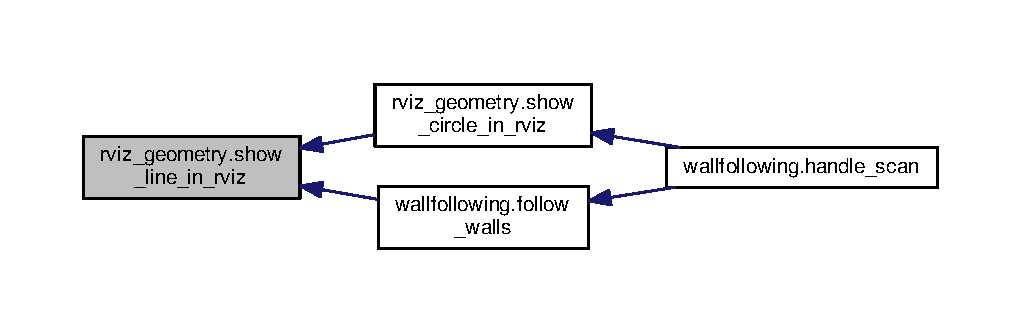
\includegraphics[width=350pt]{namespacerviz__geometry_a93390c23bebf8db38c31f832225dddda_icgraph}
\end{center}
\end{figure}




\subsection{Variable Documentation}
\index{rviz\+\_\+geometry@{rviz\+\_\+geometry}!marker\+\_\+publisher@{marker\+\_\+publisher}}
\index{marker\+\_\+publisher@{marker\+\_\+publisher}!rviz\+\_\+geometry@{rviz\+\_\+geometry}}
\subsubsection[{\texorpdfstring{marker\+\_\+publisher}{marker_publisher}}]{\setlength{\rightskip}{0pt plus 5cm}rviz\+\_\+geometry.\+marker\+\_\+publisher = rospy.\+Publisher({\bf R\+V\+I\+Z\+\_\+\+T\+O\+P\+IC}, Marker, queue\+\_\+size=1)}\hypertarget{namespacerviz__geometry_ac4b20d63343627f7ac14151eba108ba8}{}\label{namespacerviz__geometry_ac4b20d63343627f7ac14151eba108ba8}


Definition at line 13 of file rviz\+\_\+geometry.\+py.

\index{rviz\+\_\+geometry@{rviz\+\_\+geometry}!R\+V\+I\+Z\+\_\+\+F\+R\+A\+ME@{R\+V\+I\+Z\+\_\+\+F\+R\+A\+ME}}
\index{R\+V\+I\+Z\+\_\+\+F\+R\+A\+ME@{R\+V\+I\+Z\+\_\+\+F\+R\+A\+ME}!rviz\+\_\+geometry@{rviz\+\_\+geometry}}
\subsubsection[{\texorpdfstring{R\+V\+I\+Z\+\_\+\+F\+R\+A\+ME}{RVIZ_FRAME}}]{\setlength{\rightskip}{0pt plus 5cm}string rviz\+\_\+geometry.\+R\+V\+I\+Z\+\_\+\+F\+R\+A\+ME = \char`\"{}laser\char`\"{}}\hypertarget{namespacerviz__geometry_a3a3837887cc012683c1d87e5027b6863}{}\label{namespacerviz__geometry_a3a3837887cc012683c1d87e5027b6863}


Definition at line 10 of file rviz\+\_\+geometry.\+py.

\index{rviz\+\_\+geometry@{rviz\+\_\+geometry}!R\+V\+I\+Z\+\_\+\+N\+A\+M\+E\+S\+P\+A\+CE@{R\+V\+I\+Z\+\_\+\+N\+A\+M\+E\+S\+P\+A\+CE}}
\index{R\+V\+I\+Z\+\_\+\+N\+A\+M\+E\+S\+P\+A\+CE@{R\+V\+I\+Z\+\_\+\+N\+A\+M\+E\+S\+P\+A\+CE}!rviz\+\_\+geometry@{rviz\+\_\+geometry}}
\subsubsection[{\texorpdfstring{R\+V\+I\+Z\+\_\+\+N\+A\+M\+E\+S\+P\+A\+CE}{RVIZ_NAMESPACE}}]{\setlength{\rightskip}{0pt plus 5cm}string rviz\+\_\+geometry.\+R\+V\+I\+Z\+\_\+\+N\+A\+M\+E\+S\+P\+A\+CE = \char`\"{}wall\+\_\+following\char`\"{}}\hypertarget{namespacerviz__geometry_ad8626a9cfbc948e43f401fb1f3d62ecb}{}\label{namespacerviz__geometry_ad8626a9cfbc948e43f401fb1f3d62ecb}


Definition at line 11 of file rviz\+\_\+geometry.\+py.

\index{rviz\+\_\+geometry@{rviz\+\_\+geometry}!R\+V\+I\+Z\+\_\+\+T\+O\+P\+IC@{R\+V\+I\+Z\+\_\+\+T\+O\+P\+IC}}
\index{R\+V\+I\+Z\+\_\+\+T\+O\+P\+IC@{R\+V\+I\+Z\+\_\+\+T\+O\+P\+IC}!rviz\+\_\+geometry@{rviz\+\_\+geometry}}
\subsubsection[{\texorpdfstring{R\+V\+I\+Z\+\_\+\+T\+O\+P\+IC}{RVIZ_TOPIC}}]{\setlength{\rightskip}{0pt plus 5cm}string rviz\+\_\+geometry.\+R\+V\+I\+Z\+\_\+\+T\+O\+P\+IC = \char`\"{}/wallfollowing\+\_\+visualization\char`\"{}}\hypertarget{namespacerviz__geometry_a2bfe028bdabf1321495ece3cfc6b4fa6}{}\label{namespacerviz__geometry_a2bfe028bdabf1321495ece3cfc6b4fa6}


Definition at line 9 of file rviz\+\_\+geometry.\+py.


\hypertarget{namespacesetup}{}\section{setup Namespace Reference}
\label{namespacesetup}\index{setup@{setup}}
\subsection*{Variables}
\begin{DoxyCompactItemize}
\item 
\hyperlink{namespacesetup_a504ffa482edfe0eff08f64b2f5dff0e9}{setup\+\_\+args}
\end{DoxyCompactItemize}


\subsection{Variable Documentation}
\index{setup@{setup}!setup\+\_\+args@{setup\+\_\+args}}
\index{setup\+\_\+args@{setup\+\_\+args}!setup@{setup}}
\subsubsection[{\texorpdfstring{setup\+\_\+args}{setup_args}}]{\setlength{\rightskip}{0pt plus 5cm}setup.\+setup\+\_\+args}\hypertarget{namespacesetup_a504ffa482edfe0eff08f64b2f5dff0e9}{}\label{namespacesetup_a504ffa482edfe0eff08f64b2f5dff0e9}
{\bfseries Initial value\+:}
\begin{DoxyCode}
1 = generate\_distutils\_setup(
2     packages=[\textcolor{stringliteral}{'simulation\_tools'}],
3     package\_dir=\{\textcolor{stringliteral}{''}: \textcolor{stringliteral}{'src'}\}
4 )
\end{DoxyCode}


Definition at line 6 of file setup.\+py.


\hypertarget{namespacesimulation}{}\section{simulation Namespace Reference}
\label{namespacesimulation}\index{simulation@{simulation}}
\subsection*{Variables}
\begin{DoxyCompactItemize}
\item 
constexpr const char $\ast$ \hyperlink{namespacesimulation_a7a04e98990d834217946c9be604088ee}{W\+H\+E\+E\+L\+\_\+\+L\+E\+F\+T\+\_\+\+B\+A\+C\+K\+\_\+\+V\+E\+L\+O\+C\+I\+TY} = \char`\"{}/racer/left\+\_\+wheel\+\_\+back\+\_\+velocity\+\_\+controller/command\char`\"{}
\item 
constexpr const char $\ast$ \hyperlink{namespacesimulation_a84bf4fa7350ff11e42c56e6e1cf3838f}{W\+H\+E\+E\+L\+\_\+\+L\+E\+F\+T\+\_\+\+F\+R\+O\+N\+T\+\_\+\+V\+E\+L\+O\+C\+I\+TY} = \char`\"{}/racer/left\+\_\+wheel\+\_\+front\+\_\+velocity\+\_\+controller/command\char`\"{}
\item 
constexpr const char $\ast$ \hyperlink{namespacesimulation_a9b9a90d860017663afa773f15612b44e}{W\+H\+E\+E\+L\+\_\+\+R\+I\+G\+H\+T\+\_\+\+B\+A\+C\+K\+\_\+\+V\+E\+L\+O\+C\+I\+TY} = \char`\"{}/racer/right\+\_\+wheel\+\_\+back\+\_\+velocity\+\_\+controller/command\char`\"{}
\item 
constexpr const char $\ast$ \hyperlink{namespacesimulation_aad00b40febd3e9442560a15cd5204a46}{W\+H\+E\+E\+L\+\_\+\+R\+I\+G\+H\+T\+\_\+\+F\+R\+O\+N\+T\+\_\+\+V\+E\+L\+O\+C\+I\+TY} = \char`\"{}/racer/right\+\_\+wheel\+\_\+front\+\_\+velocity\+\_\+controller/command\char`\"{}
\item 
constexpr const char $\ast$ \hyperlink{namespacesimulation_aeabd7d3863831a7fc50ce8728ca46885}{L\+E\+F\+T\+\_\+\+S\+T\+E\+E\+R\+I\+N\+G\+\_\+\+P\+O\+S\+I\+T\+I\+ON} = \char`\"{}/racer/left\+\_\+steering\+\_\+hinge\+\_\+position\+\_\+controller/command\char`\"{}
\item 
constexpr const char $\ast$ \hyperlink{namespacesimulation_af34d70ba82e8343343521a32e5f6b12a}{R\+I\+G\+H\+T\+\_\+\+S\+T\+E\+E\+R\+I\+N\+G\+\_\+\+P\+O\+S\+I\+T\+I\+ON} = \char`\"{}/racer/right\+\_\+steering\+\_\+hinge\+\_\+position\+\_\+controller/command\char`\"{}
\end{DoxyCompactItemize}


\subsection{Variable Documentation}
\index{simulation@{simulation}!L\+E\+F\+T\+\_\+\+S\+T\+E\+E\+R\+I\+N\+G\+\_\+\+P\+O\+S\+I\+T\+I\+ON@{L\+E\+F\+T\+\_\+\+S\+T\+E\+E\+R\+I\+N\+G\+\_\+\+P\+O\+S\+I\+T\+I\+ON}}
\index{L\+E\+F\+T\+\_\+\+S\+T\+E\+E\+R\+I\+N\+G\+\_\+\+P\+O\+S\+I\+T\+I\+ON@{L\+E\+F\+T\+\_\+\+S\+T\+E\+E\+R\+I\+N\+G\+\_\+\+P\+O\+S\+I\+T\+I\+ON}!simulation@{simulation}}
\subsubsection[{\texorpdfstring{L\+E\+F\+T\+\_\+\+S\+T\+E\+E\+R\+I\+N\+G\+\_\+\+P\+O\+S\+I\+T\+I\+ON}{LEFT_STEERING_POSITION}}]{\setlength{\rightskip}{0pt plus 5cm}constexpr const char$\ast$ simulation\+::\+L\+E\+F\+T\+\_\+\+S\+T\+E\+E\+R\+I\+N\+G\+\_\+\+P\+O\+S\+I\+T\+I\+ON = \char`\"{}/racer/left\+\_\+steering\+\_\+hinge\+\_\+position\+\_\+controller/command\char`\"{}}\hypertarget{namespacesimulation_aeabd7d3863831a7fc50ce8728ca46885}{}\label{namespacesimulation_aeabd7d3863831a7fc50ce8728ca46885}


Definition at line 22 of file vesc\+\_\+sim\+\_\+driver.\+h.

\index{simulation@{simulation}!R\+I\+G\+H\+T\+\_\+\+S\+T\+E\+E\+R\+I\+N\+G\+\_\+\+P\+O\+S\+I\+T\+I\+ON@{R\+I\+G\+H\+T\+\_\+\+S\+T\+E\+E\+R\+I\+N\+G\+\_\+\+P\+O\+S\+I\+T\+I\+ON}}
\index{R\+I\+G\+H\+T\+\_\+\+S\+T\+E\+E\+R\+I\+N\+G\+\_\+\+P\+O\+S\+I\+T\+I\+ON@{R\+I\+G\+H\+T\+\_\+\+S\+T\+E\+E\+R\+I\+N\+G\+\_\+\+P\+O\+S\+I\+T\+I\+ON}!simulation@{simulation}}
\subsubsection[{\texorpdfstring{R\+I\+G\+H\+T\+\_\+\+S\+T\+E\+E\+R\+I\+N\+G\+\_\+\+P\+O\+S\+I\+T\+I\+ON}{RIGHT_STEERING_POSITION}}]{\setlength{\rightskip}{0pt plus 5cm}constexpr const char$\ast$ simulation\+::\+R\+I\+G\+H\+T\+\_\+\+S\+T\+E\+E\+R\+I\+N\+G\+\_\+\+P\+O\+S\+I\+T\+I\+ON = \char`\"{}/racer/right\+\_\+steering\+\_\+hinge\+\_\+position\+\_\+controller/command\char`\"{}}\hypertarget{namespacesimulation_af34d70ba82e8343343521a32e5f6b12a}{}\label{namespacesimulation_af34d70ba82e8343343521a32e5f6b12a}


Definition at line 23 of file vesc\+\_\+sim\+\_\+driver.\+h.

\index{simulation@{simulation}!W\+H\+E\+E\+L\+\_\+\+L\+E\+F\+T\+\_\+\+B\+A\+C\+K\+\_\+\+V\+E\+L\+O\+C\+I\+TY@{W\+H\+E\+E\+L\+\_\+\+L\+E\+F\+T\+\_\+\+B\+A\+C\+K\+\_\+\+V\+E\+L\+O\+C\+I\+TY}}
\index{W\+H\+E\+E\+L\+\_\+\+L\+E\+F\+T\+\_\+\+B\+A\+C\+K\+\_\+\+V\+E\+L\+O\+C\+I\+TY@{W\+H\+E\+E\+L\+\_\+\+L\+E\+F\+T\+\_\+\+B\+A\+C\+K\+\_\+\+V\+E\+L\+O\+C\+I\+TY}!simulation@{simulation}}
\subsubsection[{\texorpdfstring{W\+H\+E\+E\+L\+\_\+\+L\+E\+F\+T\+\_\+\+B\+A\+C\+K\+\_\+\+V\+E\+L\+O\+C\+I\+TY}{WHEEL_LEFT_BACK_VELOCITY}}]{\setlength{\rightskip}{0pt plus 5cm}constexpr const char$\ast$ simulation\+::\+W\+H\+E\+E\+L\+\_\+\+L\+E\+F\+T\+\_\+\+B\+A\+C\+K\+\_\+\+V\+E\+L\+O\+C\+I\+TY = \char`\"{}/racer/left\+\_\+wheel\+\_\+back\+\_\+velocity\+\_\+controller/command\char`\"{}}\hypertarget{namespacesimulation_a7a04e98990d834217946c9be604088ee}{}\label{namespacesimulation_a7a04e98990d834217946c9be604088ee}


Definition at line 18 of file vesc\+\_\+sim\+\_\+driver.\+h.

\index{simulation@{simulation}!W\+H\+E\+E\+L\+\_\+\+L\+E\+F\+T\+\_\+\+F\+R\+O\+N\+T\+\_\+\+V\+E\+L\+O\+C\+I\+TY@{W\+H\+E\+E\+L\+\_\+\+L\+E\+F\+T\+\_\+\+F\+R\+O\+N\+T\+\_\+\+V\+E\+L\+O\+C\+I\+TY}}
\index{W\+H\+E\+E\+L\+\_\+\+L\+E\+F\+T\+\_\+\+F\+R\+O\+N\+T\+\_\+\+V\+E\+L\+O\+C\+I\+TY@{W\+H\+E\+E\+L\+\_\+\+L\+E\+F\+T\+\_\+\+F\+R\+O\+N\+T\+\_\+\+V\+E\+L\+O\+C\+I\+TY}!simulation@{simulation}}
\subsubsection[{\texorpdfstring{W\+H\+E\+E\+L\+\_\+\+L\+E\+F\+T\+\_\+\+F\+R\+O\+N\+T\+\_\+\+V\+E\+L\+O\+C\+I\+TY}{WHEEL_LEFT_FRONT_VELOCITY}}]{\setlength{\rightskip}{0pt plus 5cm}constexpr const char$\ast$ simulation\+::\+W\+H\+E\+E\+L\+\_\+\+L\+E\+F\+T\+\_\+\+F\+R\+O\+N\+T\+\_\+\+V\+E\+L\+O\+C\+I\+TY = \char`\"{}/racer/left\+\_\+wheel\+\_\+front\+\_\+velocity\+\_\+controller/command\char`\"{}}\hypertarget{namespacesimulation_a84bf4fa7350ff11e42c56e6e1cf3838f}{}\label{namespacesimulation_a84bf4fa7350ff11e42c56e6e1cf3838f}


Definition at line 19 of file vesc\+\_\+sim\+\_\+driver.\+h.

\index{simulation@{simulation}!W\+H\+E\+E\+L\+\_\+\+R\+I\+G\+H\+T\+\_\+\+B\+A\+C\+K\+\_\+\+V\+E\+L\+O\+C\+I\+TY@{W\+H\+E\+E\+L\+\_\+\+R\+I\+G\+H\+T\+\_\+\+B\+A\+C\+K\+\_\+\+V\+E\+L\+O\+C\+I\+TY}}
\index{W\+H\+E\+E\+L\+\_\+\+R\+I\+G\+H\+T\+\_\+\+B\+A\+C\+K\+\_\+\+V\+E\+L\+O\+C\+I\+TY@{W\+H\+E\+E\+L\+\_\+\+R\+I\+G\+H\+T\+\_\+\+B\+A\+C\+K\+\_\+\+V\+E\+L\+O\+C\+I\+TY}!simulation@{simulation}}
\subsubsection[{\texorpdfstring{W\+H\+E\+E\+L\+\_\+\+R\+I\+G\+H\+T\+\_\+\+B\+A\+C\+K\+\_\+\+V\+E\+L\+O\+C\+I\+TY}{WHEEL_RIGHT_BACK_VELOCITY}}]{\setlength{\rightskip}{0pt plus 5cm}constexpr const char$\ast$ simulation\+::\+W\+H\+E\+E\+L\+\_\+\+R\+I\+G\+H\+T\+\_\+\+B\+A\+C\+K\+\_\+\+V\+E\+L\+O\+C\+I\+TY = \char`\"{}/racer/right\+\_\+wheel\+\_\+back\+\_\+velocity\+\_\+controller/command\char`\"{}}\hypertarget{namespacesimulation_a9b9a90d860017663afa773f15612b44e}{}\label{namespacesimulation_a9b9a90d860017663afa773f15612b44e}


Definition at line 20 of file vesc\+\_\+sim\+\_\+driver.\+h.

\index{simulation@{simulation}!W\+H\+E\+E\+L\+\_\+\+R\+I\+G\+H\+T\+\_\+\+F\+R\+O\+N\+T\+\_\+\+V\+E\+L\+O\+C\+I\+TY@{W\+H\+E\+E\+L\+\_\+\+R\+I\+G\+H\+T\+\_\+\+F\+R\+O\+N\+T\+\_\+\+V\+E\+L\+O\+C\+I\+TY}}
\index{W\+H\+E\+E\+L\+\_\+\+R\+I\+G\+H\+T\+\_\+\+F\+R\+O\+N\+T\+\_\+\+V\+E\+L\+O\+C\+I\+TY@{W\+H\+E\+E\+L\+\_\+\+R\+I\+G\+H\+T\+\_\+\+F\+R\+O\+N\+T\+\_\+\+V\+E\+L\+O\+C\+I\+TY}!simulation@{simulation}}
\subsubsection[{\texorpdfstring{W\+H\+E\+E\+L\+\_\+\+R\+I\+G\+H\+T\+\_\+\+F\+R\+O\+N\+T\+\_\+\+V\+E\+L\+O\+C\+I\+TY}{WHEEL_RIGHT_FRONT_VELOCITY}}]{\setlength{\rightskip}{0pt plus 5cm}constexpr const char$\ast$ simulation\+::\+W\+H\+E\+E\+L\+\_\+\+R\+I\+G\+H\+T\+\_\+\+F\+R\+O\+N\+T\+\_\+\+V\+E\+L\+O\+C\+I\+TY = \char`\"{}/racer/right\+\_\+wheel\+\_\+front\+\_\+velocity\+\_\+controller/command\char`\"{}}\hypertarget{namespacesimulation_aad00b40febd3e9442560a15cd5204a46}{}\label{namespacesimulation_aad00b40febd3e9442560a15cd5204a46}


Definition at line 21 of file vesc\+\_\+sim\+\_\+driver.\+h.


\hypertarget{namespacesimulation__tools}{}\section{simulation\+\_\+tools Namespace Reference}
\label{namespacesimulation__tools}\index{simulation\+\_\+tools@{simulation\+\_\+tools}}
\subsection*{Namespaces}
\begin{DoxyCompactItemize}
\item 
 \hyperlink{namespacesimulation__tools_1_1lap__timer}{lap\+\_\+timer}
\item 
 \hyperlink{namespacesimulation__tools_1_1reset__car}{reset\+\_\+car}
\item 
 \hyperlink{namespacesimulation__tools_1_1speedometer}{speedometer}
\item 
 \hyperlink{namespacesimulation__tools_1_1track}{track}
\end{DoxyCompactItemize}

\hypertarget{namespacesimulation__tools_1_1lap__timer}{}\section{simulation\+\_\+tools.\+lap\+\_\+timer Namespace Reference}
\label{namespacesimulation__tools_1_1lap__timer}\index{simulation\+\_\+tools.\+lap\+\_\+timer@{simulation\+\_\+tools.\+lap\+\_\+timer}}
\subsection*{Classes}
\begin{DoxyCompactItemize}
\item 
class \hyperlink{classsimulation__tools_1_1lap__timer_1_1_area}{Area}
\item 
class \hyperlink{classsimulation__tools_1_1lap__timer_1_1_timer}{Timer}
\end{DoxyCompactItemize}
\subsection*{Functions}
\begin{DoxyCompactItemize}
\item 
def \hyperlink{namespacesimulation__tools_1_1lap__timer_a8ff1f7d7789d5ea92df79c94205a7273}{format\+\_\+duration} (duration)
\item 
def \hyperlink{namespacesimulation__tools_1_1lap__timer_adb38c2045a967ab6f7c0c6968599c2ff}{model\+\_\+state\+\_\+callback} (message)
\end{DoxyCompactItemize}
\subsection*{Variables}
\begin{DoxyCompactItemize}
\item 
\hyperlink{namespacesimulation__tools_1_1lap__timer_a55d342023a9bdc266a2ee262040e8d19}{Point} = namedtuple(\char`\"{}Point\char`\"{}, \mbox{[}\char`\"{}x\char`\"{}, \char`\"{}y\char`\"{}\mbox{]})
\item 
\hyperlink{namespacesimulation__tools_1_1lap__timer_ae7d1eef6c19d3320b71be19367ec7fbd}{F\+I\+N\+I\+S\+H\+\_\+\+L\+I\+N\+E\+\_\+1} = \hyperlink{classsimulation__tools_1_1lap__timer_1_1_area}{Area}(\hyperlink{namespacesimulation__tools_1_1lap__timer_a55d342023a9bdc266a2ee262040e8d19}{Point}(0, -\/0.\+5), \hyperlink{namespacesimulation__tools_1_1lap__timer_a55d342023a9bdc266a2ee262040e8d19}{Point}(2.\+8, 1))
\item 
\hyperlink{namespacesimulation__tools_1_1lap__timer_ac066eea03916600e5942b91bba4204fa}{F\+I\+N\+I\+S\+H\+\_\+\+L\+I\+N\+E\+\_\+2} = \hyperlink{classsimulation__tools_1_1lap__timer_1_1_area}{Area}(\hyperlink{namespacesimulation__tools_1_1lap__timer_a55d342023a9bdc266a2ee262040e8d19}{Point}(4, -\/0.\+5), \hyperlink{namespacesimulation__tools_1_1lap__timer_a55d342023a9bdc266a2ee262040e8d19}{Point}(1.\+2, 1))
\item 
\hyperlink{namespacesimulation__tools_1_1lap__timer_a20574c968e10b9baa7bb953a9a7eb693}{C\+H\+E\+C\+K\+P\+O\+I\+N\+T\+\_\+1} = \hyperlink{classsimulation__tools_1_1lap__timer_1_1_area}{Area}(\hyperlink{namespacesimulation__tools_1_1lap__timer_a55d342023a9bdc266a2ee262040e8d19}{Point}(11, 7), \hyperlink{namespacesimulation__tools_1_1lap__timer_a55d342023a9bdc266a2ee262040e8d19}{Point}(2, 2))
\item 
\hyperlink{namespacesimulation__tools_1_1lap__timer_a7773acfe8635b4d8a0e96d13912243b0}{C\+H\+E\+C\+K\+P\+O\+I\+N\+T\+\_\+2} = \hyperlink{classsimulation__tools_1_1lap__timer_1_1_area}{Area}(\hyperlink{namespacesimulation__tools_1_1lap__timer_a55d342023a9bdc266a2ee262040e8d19}{Point}(0, 4), \hyperlink{namespacesimulation__tools_1_1lap__timer_a55d342023a9bdc266a2ee262040e8d19}{Point}(2, 2))
\item 
\hyperlink{namespacesimulation__tools_1_1lap__timer_a197a8c1ba2497108f555aa4d1670ccd7}{C\+H\+E\+C\+K\+P\+O\+I\+N\+T\+\_\+3} = \hyperlink{classsimulation__tools_1_1lap__timer_1_1_area}{Area}(\hyperlink{namespacesimulation__tools_1_1lap__timer_a55d342023a9bdc266a2ee262040e8d19}{Point}(-\/14, 1), \hyperlink{namespacesimulation__tools_1_1lap__timer_a55d342023a9bdc266a2ee262040e8d19}{Point}(2, 2))
\item 
\hyperlink{namespacesimulation__tools_1_1lap__timer_aab75b520d524490f7b0bdcf6b28761a6}{forward\+\_\+track}
\item 
\hyperlink{namespacesimulation__tools_1_1lap__timer_a05166a035886cf7f2693a8f72dc05bbc}{reverse\+\_\+track}
\end{DoxyCompactItemize}


\subsection{Function Documentation}
\index{simulation\+\_\+tools\+::lap\+\_\+timer@{simulation\+\_\+tools\+::lap\+\_\+timer}!format\+\_\+duration@{format\+\_\+duration}}
\index{format\+\_\+duration@{format\+\_\+duration}!simulation\+\_\+tools\+::lap\+\_\+timer@{simulation\+\_\+tools\+::lap\+\_\+timer}}
\subsubsection[{\texorpdfstring{format\+\_\+duration(duration)}{format_duration(duration)}}]{\setlength{\rightskip}{0pt plus 5cm}def simulation\+\_\+tools.\+lap\+\_\+timer.\+format\+\_\+duration (
\begin{DoxyParamCaption}
\item[{}]{duration}
\end{DoxyParamCaption}
)}\hypertarget{namespacesimulation__tools_1_1lap__timer_a8ff1f7d7789d5ea92df79c94205a7273}{}\label{namespacesimulation__tools_1_1lap__timer_a8ff1f7d7789d5ea92df79c94205a7273}


Definition at line 12 of file lap\+\_\+timer.\+py.



Here is the caller graph for this function\+:
\nopagebreak
\begin{figure}[H]
\begin{center}
\leavevmode
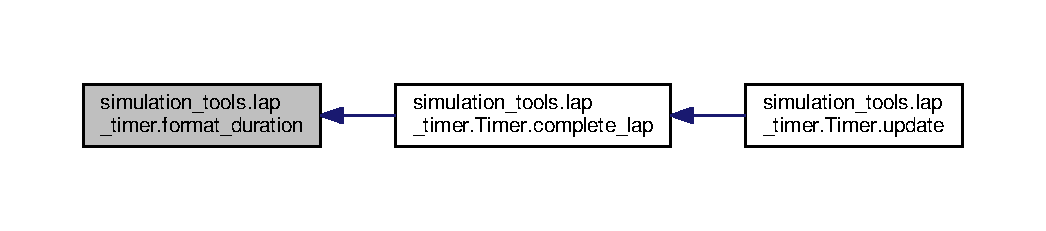
\includegraphics[width=350pt]{namespacesimulation__tools_1_1lap__timer_a8ff1f7d7789d5ea92df79c94205a7273_icgraph}
\end{center}
\end{figure}


\index{simulation\+\_\+tools\+::lap\+\_\+timer@{simulation\+\_\+tools\+::lap\+\_\+timer}!model\+\_\+state\+\_\+callback@{model\+\_\+state\+\_\+callback}}
\index{model\+\_\+state\+\_\+callback@{model\+\_\+state\+\_\+callback}!simulation\+\_\+tools\+::lap\+\_\+timer@{simulation\+\_\+tools\+::lap\+\_\+timer}}
\subsubsection[{\texorpdfstring{model\+\_\+state\+\_\+callback(message)}{model_state_callback(message)}}]{\setlength{\rightskip}{0pt plus 5cm}def simulation\+\_\+tools.\+lap\+\_\+timer.\+model\+\_\+state\+\_\+callback (
\begin{DoxyParamCaption}
\item[{}]{message}
\end{DoxyParamCaption}
)}\hypertarget{namespacesimulation__tools_1_1lap__timer_adb38c2045a967ab6f7c0c6968599c2ff}{}\label{namespacesimulation__tools_1_1lap__timer_adb38c2045a967ab6f7c0c6968599c2ff}


Definition at line 91 of file lap\+\_\+timer.\+py.



\subsection{Variable Documentation}
\index{simulation\+\_\+tools\+::lap\+\_\+timer@{simulation\+\_\+tools\+::lap\+\_\+timer}!C\+H\+E\+C\+K\+P\+O\+I\+N\+T\+\_\+1@{C\+H\+E\+C\+K\+P\+O\+I\+N\+T\+\_\+1}}
\index{C\+H\+E\+C\+K\+P\+O\+I\+N\+T\+\_\+1@{C\+H\+E\+C\+K\+P\+O\+I\+N\+T\+\_\+1}!simulation\+\_\+tools\+::lap\+\_\+timer@{simulation\+\_\+tools\+::lap\+\_\+timer}}
\subsubsection[{\texorpdfstring{C\+H\+E\+C\+K\+P\+O\+I\+N\+T\+\_\+1}{CHECKPOINT_1}}]{\setlength{\rightskip}{0pt plus 5cm}simulation\+\_\+tools.\+lap\+\_\+timer.\+C\+H\+E\+C\+K\+P\+O\+I\+N\+T\+\_\+1 = {\bf Area}({\bf Point}(11, 7), {\bf Point}(2, 2))}\hypertarget{namespacesimulation__tools_1_1lap__timer_a20574c968e10b9baa7bb953a9a7eb693}{}\label{namespacesimulation__tools_1_1lap__timer_a20574c968e10b9baa7bb953a9a7eb693}


Definition at line 68 of file lap\+\_\+timer.\+py.

\index{simulation\+\_\+tools\+::lap\+\_\+timer@{simulation\+\_\+tools\+::lap\+\_\+timer}!C\+H\+E\+C\+K\+P\+O\+I\+N\+T\+\_\+2@{C\+H\+E\+C\+K\+P\+O\+I\+N\+T\+\_\+2}}
\index{C\+H\+E\+C\+K\+P\+O\+I\+N\+T\+\_\+2@{C\+H\+E\+C\+K\+P\+O\+I\+N\+T\+\_\+2}!simulation\+\_\+tools\+::lap\+\_\+timer@{simulation\+\_\+tools\+::lap\+\_\+timer}}
\subsubsection[{\texorpdfstring{C\+H\+E\+C\+K\+P\+O\+I\+N\+T\+\_\+2}{CHECKPOINT_2}}]{\setlength{\rightskip}{0pt plus 5cm}simulation\+\_\+tools.\+lap\+\_\+timer.\+C\+H\+E\+C\+K\+P\+O\+I\+N\+T\+\_\+2 = {\bf Area}({\bf Point}(0, 4), {\bf Point}(2, 2))}\hypertarget{namespacesimulation__tools_1_1lap__timer_a7773acfe8635b4d8a0e96d13912243b0}{}\label{namespacesimulation__tools_1_1lap__timer_a7773acfe8635b4d8a0e96d13912243b0}


Definition at line 69 of file lap\+\_\+timer.\+py.

\index{simulation\+\_\+tools\+::lap\+\_\+timer@{simulation\+\_\+tools\+::lap\+\_\+timer}!C\+H\+E\+C\+K\+P\+O\+I\+N\+T\+\_\+3@{C\+H\+E\+C\+K\+P\+O\+I\+N\+T\+\_\+3}}
\index{C\+H\+E\+C\+K\+P\+O\+I\+N\+T\+\_\+3@{C\+H\+E\+C\+K\+P\+O\+I\+N\+T\+\_\+3}!simulation\+\_\+tools\+::lap\+\_\+timer@{simulation\+\_\+tools\+::lap\+\_\+timer}}
\subsubsection[{\texorpdfstring{C\+H\+E\+C\+K\+P\+O\+I\+N\+T\+\_\+3}{CHECKPOINT_3}}]{\setlength{\rightskip}{0pt plus 5cm}simulation\+\_\+tools.\+lap\+\_\+timer.\+C\+H\+E\+C\+K\+P\+O\+I\+N\+T\+\_\+3 = {\bf Area}({\bf Point}(-\/14, 1), {\bf Point}(2, 2))}\hypertarget{namespacesimulation__tools_1_1lap__timer_a197a8c1ba2497108f555aa4d1670ccd7}{}\label{namespacesimulation__tools_1_1lap__timer_a197a8c1ba2497108f555aa4d1670ccd7}


Definition at line 70 of file lap\+\_\+timer.\+py.

\index{simulation\+\_\+tools\+::lap\+\_\+timer@{simulation\+\_\+tools\+::lap\+\_\+timer}!F\+I\+N\+I\+S\+H\+\_\+\+L\+I\+N\+E\+\_\+1@{F\+I\+N\+I\+S\+H\+\_\+\+L\+I\+N\+E\+\_\+1}}
\index{F\+I\+N\+I\+S\+H\+\_\+\+L\+I\+N\+E\+\_\+1@{F\+I\+N\+I\+S\+H\+\_\+\+L\+I\+N\+E\+\_\+1}!simulation\+\_\+tools\+::lap\+\_\+timer@{simulation\+\_\+tools\+::lap\+\_\+timer}}
\subsubsection[{\texorpdfstring{F\+I\+N\+I\+S\+H\+\_\+\+L\+I\+N\+E\+\_\+1}{FINISH_LINE_1}}]{\setlength{\rightskip}{0pt plus 5cm}simulation\+\_\+tools.\+lap\+\_\+timer.\+F\+I\+N\+I\+S\+H\+\_\+\+L\+I\+N\+E\+\_\+1 = {\bf Area}({\bf Point}(0, -\/0.\+5), {\bf Point}(2.\+8, 1))}\hypertarget{namespacesimulation__tools_1_1lap__timer_ae7d1eef6c19d3320b71be19367ec7fbd}{}\label{namespacesimulation__tools_1_1lap__timer_ae7d1eef6c19d3320b71be19367ec7fbd}


Definition at line 66 of file lap\+\_\+timer.\+py.

\index{simulation\+\_\+tools\+::lap\+\_\+timer@{simulation\+\_\+tools\+::lap\+\_\+timer}!F\+I\+N\+I\+S\+H\+\_\+\+L\+I\+N\+E\+\_\+2@{F\+I\+N\+I\+S\+H\+\_\+\+L\+I\+N\+E\+\_\+2}}
\index{F\+I\+N\+I\+S\+H\+\_\+\+L\+I\+N\+E\+\_\+2@{F\+I\+N\+I\+S\+H\+\_\+\+L\+I\+N\+E\+\_\+2}!simulation\+\_\+tools\+::lap\+\_\+timer@{simulation\+\_\+tools\+::lap\+\_\+timer}}
\subsubsection[{\texorpdfstring{F\+I\+N\+I\+S\+H\+\_\+\+L\+I\+N\+E\+\_\+2}{FINISH_LINE_2}}]{\setlength{\rightskip}{0pt plus 5cm}simulation\+\_\+tools.\+lap\+\_\+timer.\+F\+I\+N\+I\+S\+H\+\_\+\+L\+I\+N\+E\+\_\+2 = {\bf Area}({\bf Point}(4, -\/0.\+5), {\bf Point}(1.\+2, 1))}\hypertarget{namespacesimulation__tools_1_1lap__timer_ac066eea03916600e5942b91bba4204fa}{}\label{namespacesimulation__tools_1_1lap__timer_ac066eea03916600e5942b91bba4204fa}


Definition at line 67 of file lap\+\_\+timer.\+py.

\index{simulation\+\_\+tools\+::lap\+\_\+timer@{simulation\+\_\+tools\+::lap\+\_\+timer}!forward\+\_\+track@{forward\+\_\+track}}
\index{forward\+\_\+track@{forward\+\_\+track}!simulation\+\_\+tools\+::lap\+\_\+timer@{simulation\+\_\+tools\+::lap\+\_\+timer}}
\subsubsection[{\texorpdfstring{forward\+\_\+track}{forward_track}}]{\setlength{\rightskip}{0pt plus 5cm}simulation\+\_\+tools.\+lap\+\_\+timer.\+forward\+\_\+track}\hypertarget{namespacesimulation__tools_1_1lap__timer_aab75b520d524490f7b0bdcf6b28761a6}{}\label{namespacesimulation__tools_1_1lap__timer_aab75b520d524490f7b0bdcf6b28761a6}
{\bfseries Initial value\+:}
\begin{DoxyCode}
1 = \hyperlink{classsimulation__tools_1_1lap__timer_1_1_timer}{Timer}(\textcolor{stringliteral}{"forward"}, (
2     FINISH\_LINE\_1,
3     FINISH\_LINE\_2,
4     CHECKPOINT\_1,
5     CHECKPOINT\_2,
6     CHECKPOINT\_3,
7     FINISH\_LINE\_1,
8     FINISH\_LINE\_2))
\end{DoxyCode}


Definition at line 72 of file lap\+\_\+timer.\+py.

\index{simulation\+\_\+tools\+::lap\+\_\+timer@{simulation\+\_\+tools\+::lap\+\_\+timer}!Point@{Point}}
\index{Point@{Point}!simulation\+\_\+tools\+::lap\+\_\+timer@{simulation\+\_\+tools\+::lap\+\_\+timer}}
\subsubsection[{\texorpdfstring{Point}{Point}}]{\setlength{\rightskip}{0pt plus 5cm}simulation\+\_\+tools.\+lap\+\_\+timer.\+Point = namedtuple(\char`\"{}Point\char`\"{}, \mbox{[}\char`\"{}x\char`\"{}, \char`\"{}y\char`\"{}\mbox{]})}\hypertarget{namespacesimulation__tools_1_1lap__timer_a55d342023a9bdc266a2ee262040e8d19}{}\label{namespacesimulation__tools_1_1lap__timer_a55d342023a9bdc266a2ee262040e8d19}


Definition at line 9 of file lap\+\_\+timer.\+py.

\index{simulation\+\_\+tools\+::lap\+\_\+timer@{simulation\+\_\+tools\+::lap\+\_\+timer}!reverse\+\_\+track@{reverse\+\_\+track}}
\index{reverse\+\_\+track@{reverse\+\_\+track}!simulation\+\_\+tools\+::lap\+\_\+timer@{simulation\+\_\+tools\+::lap\+\_\+timer}}
\subsubsection[{\texorpdfstring{reverse\+\_\+track}{reverse_track}}]{\setlength{\rightskip}{0pt plus 5cm}simulation\+\_\+tools.\+lap\+\_\+timer.\+reverse\+\_\+track}\hypertarget{namespacesimulation__tools_1_1lap__timer_a05166a035886cf7f2693a8f72dc05bbc}{}\label{namespacesimulation__tools_1_1lap__timer_a05166a035886cf7f2693a8f72dc05bbc}
{\bfseries Initial value\+:}
\begin{DoxyCode}
1 = \hyperlink{classsimulation__tools_1_1lap__timer_1_1_timer}{Timer}(\textcolor{stringliteral}{"reverse"}, (
2     FINISH\_LINE\_2,
3     FINISH\_LINE\_1,
4     CHECKPOINT\_3,
5     CHECKPOINT\_2,
6     CHECKPOINT\_1,
7     FINISH\_LINE\_2,
8     FINISH\_LINE\_1))
\end{DoxyCode}


Definition at line 81 of file lap\+\_\+timer.\+py.


\hypertarget{namespacesimulation__tools_1_1reset__car}{}\section{simulation\+\_\+tools.\+reset\+\_\+car Namespace Reference}
\label{namespacesimulation__tools_1_1reset__car}\index{simulation\+\_\+tools.\+reset\+\_\+car@{simulation\+\_\+tools.\+reset\+\_\+car}}
\subsection*{Functions}
\begin{DoxyCompactItemize}
\item 
def \hyperlink{namespacesimulation__tools_1_1reset__car_a308f176601987becbe329e8aad7f8b88}{set\+\_\+pose} (position, orientation)
\item 
def \hyperlink{namespacesimulation__tools_1_1reset__car_a899d0894bba97bd012824d41e36395b9}{reset} (progress=0, angle=0, offset\+\_\+from\+\_\+center=0, forward=True)
\item 
def \hyperlink{namespacesimulation__tools_1_1reset__car_a4866780a44278581a356c77cd3ad6b78}{reset\+\_\+random} (max\+\_\+angle=0, max\+\_\+offset\+\_\+from\+\_\+center=0, forward=True)
\item 
def \hyperlink{namespacesimulation__tools_1_1reset__car_ac6238e711a237fd23e68e675262e7edd}{register\+\_\+service} ()
\end{DoxyCompactItemize}
\subsection*{Variables}
\begin{DoxyCompactItemize}
\item 
\hyperlink{namespacesimulation__tools_1_1reset__car_a0fcc6f9aa08bea780ef83201d5a71169}{set\+\_\+model\+\_\+state} = None
\end{DoxyCompactItemize}


\subsection{Function Documentation}
\index{simulation\+\_\+tools\+::reset\+\_\+car@{simulation\+\_\+tools\+::reset\+\_\+car}!register\+\_\+service@{register\+\_\+service}}
\index{register\+\_\+service@{register\+\_\+service}!simulation\+\_\+tools\+::reset\+\_\+car@{simulation\+\_\+tools\+::reset\+\_\+car}}
\subsubsection[{\texorpdfstring{register\+\_\+service()}{register_service()}}]{\setlength{\rightskip}{0pt plus 5cm}def simulation\+\_\+tools.\+reset\+\_\+car.\+register\+\_\+service (
\begin{DoxyParamCaption}
{}
\end{DoxyParamCaption}
)}\hypertarget{namespacesimulation__tools_1_1reset__car_ac6238e711a237fd23e68e675262e7edd}{}\label{namespacesimulation__tools_1_1reset__car_ac6238e711a237fd23e68e675262e7edd}


Definition at line 46 of file reset\+\_\+car.\+py.



Here is the call graph for this function\+:
\nopagebreak
\begin{figure}[H]
\begin{center}
\leavevmode
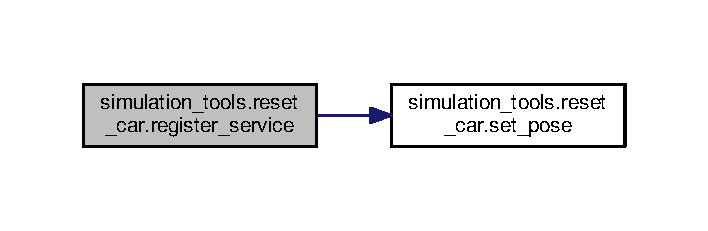
\includegraphics[width=340pt]{namespacesimulation__tools_1_1reset__car_ac6238e711a237fd23e68e675262e7edd_cgraph}
\end{center}
\end{figure}


\index{simulation\+\_\+tools\+::reset\+\_\+car@{simulation\+\_\+tools\+::reset\+\_\+car}!reset@{reset}}
\index{reset@{reset}!simulation\+\_\+tools\+::reset\+\_\+car@{simulation\+\_\+tools\+::reset\+\_\+car}}
\subsubsection[{\texorpdfstring{reset(progress=0, angle=0, offset\+\_\+from\+\_\+center=0, forward=\+True)}{reset(progress=0, angle=0, offset_from_center=0, forward=True)}}]{\setlength{\rightskip}{0pt plus 5cm}def simulation\+\_\+tools.\+reset\+\_\+car.\+reset (
\begin{DoxyParamCaption}
\item[{}]{progress = {\ttfamily 0}, }
\item[{}]{angle = {\ttfamily 0}, }
\item[{}]{offset\+\_\+from\+\_\+center = {\ttfamily 0}, }
\item[{}]{forward = {\ttfamily True}}
\end{DoxyParamCaption}
)}\hypertarget{namespacesimulation__tools_1_1reset__car_a899d0894bba97bd012824d41e36395b9}{}\label{namespacesimulation__tools_1_1reset__car_a899d0894bba97bd012824d41e36395b9}


Definition at line 30 of file reset\+\_\+car.\+py.



Here is the call graph for this function\+:
\nopagebreak
\begin{figure}[H]
\begin{center}
\leavevmode
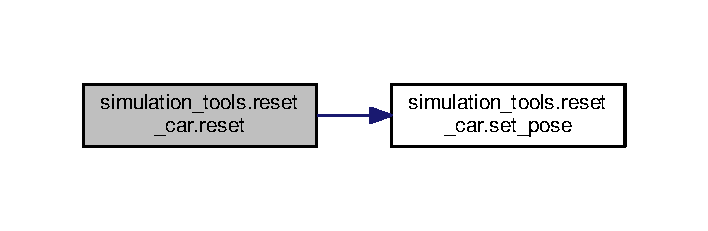
\includegraphics[width=340pt]{namespacesimulation__tools_1_1reset__car_a899d0894bba97bd012824d41e36395b9_cgraph}
\end{center}
\end{figure}




Here is the caller graph for this function\+:
\nopagebreak
\begin{figure}[H]
\begin{center}
\leavevmode
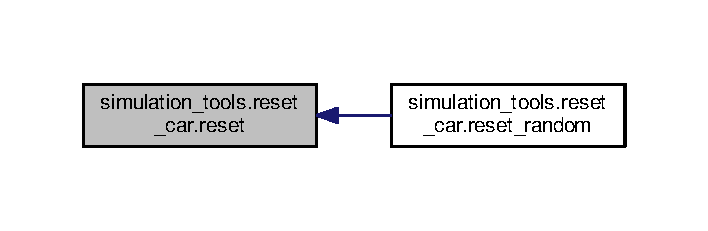
\includegraphics[width=340pt]{namespacesimulation__tools_1_1reset__car_a899d0894bba97bd012824d41e36395b9_icgraph}
\end{center}
\end{figure}


\index{simulation\+\_\+tools\+::reset\+\_\+car@{simulation\+\_\+tools\+::reset\+\_\+car}!reset\+\_\+random@{reset\+\_\+random}}
\index{reset\+\_\+random@{reset\+\_\+random}!simulation\+\_\+tools\+::reset\+\_\+car@{simulation\+\_\+tools\+::reset\+\_\+car}}
\subsubsection[{\texorpdfstring{reset\+\_\+random(max\+\_\+angle=0, max\+\_\+offset\+\_\+from\+\_\+center=0, forward=\+True)}{reset_random(max_angle=0, max_offset_from_center=0, forward=True)}}]{\setlength{\rightskip}{0pt plus 5cm}def simulation\+\_\+tools.\+reset\+\_\+car.\+reset\+\_\+random (
\begin{DoxyParamCaption}
\item[{}]{max\+\_\+angle = {\ttfamily 0}, }
\item[{}]{max\+\_\+offset\+\_\+from\+\_\+center = {\ttfamily 0}, }
\item[{}]{forward = {\ttfamily True}}
\end{DoxyParamCaption}
)}\hypertarget{namespacesimulation__tools_1_1reset__car_a4866780a44278581a356c77cd3ad6b78}{}\label{namespacesimulation__tools_1_1reset__car_a4866780a44278581a356c77cd3ad6b78}


Definition at line 38 of file reset\+\_\+car.\+py.



Here is the call graph for this function\+:
\nopagebreak
\begin{figure}[H]
\begin{center}
\leavevmode
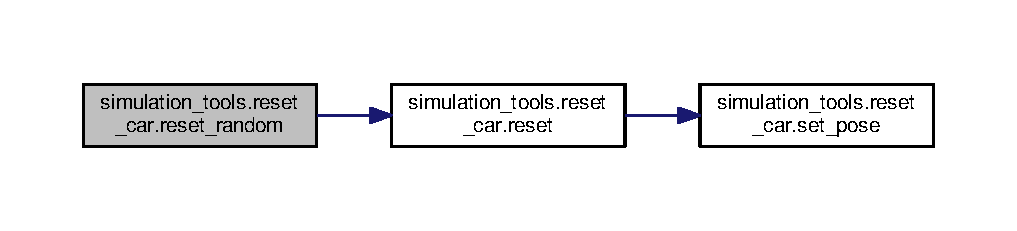
\includegraphics[width=350pt]{namespacesimulation__tools_1_1reset__car_a4866780a44278581a356c77cd3ad6b78_cgraph}
\end{center}
\end{figure}


\index{simulation\+\_\+tools\+::reset\+\_\+car@{simulation\+\_\+tools\+::reset\+\_\+car}!set\+\_\+pose@{set\+\_\+pose}}
\index{set\+\_\+pose@{set\+\_\+pose}!simulation\+\_\+tools\+::reset\+\_\+car@{simulation\+\_\+tools\+::reset\+\_\+car}}
\subsubsection[{\texorpdfstring{set\+\_\+pose(position, orientation)}{set_pose(position, orientation)}}]{\setlength{\rightskip}{0pt plus 5cm}def simulation\+\_\+tools.\+reset\+\_\+car.\+set\+\_\+pose (
\begin{DoxyParamCaption}
\item[{}]{position, }
\item[{}]{orientation}
\end{DoxyParamCaption}
)}\hypertarget{namespacesimulation__tools_1_1reset__car_a308f176601987becbe329e8aad7f8b88}{}\label{namespacesimulation__tools_1_1reset__car_a308f176601987becbe329e8aad7f8b88}


Definition at line 14 of file reset\+\_\+car.\+py.



Here is the caller graph for this function\+:
\nopagebreak
\begin{figure}[H]
\begin{center}
\leavevmode
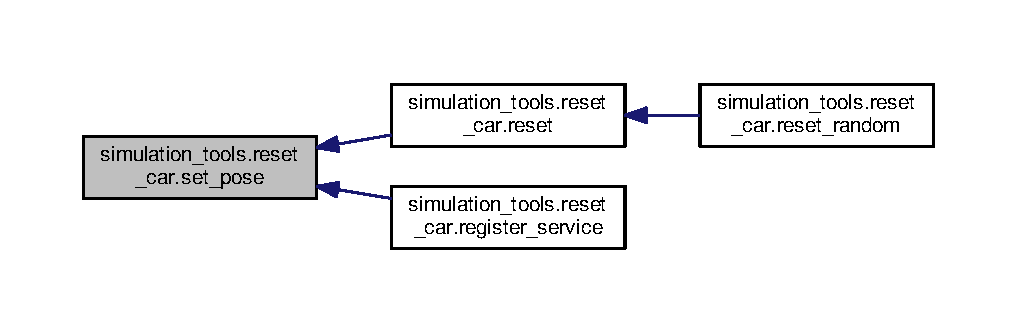
\includegraphics[width=350pt]{namespacesimulation__tools_1_1reset__car_a308f176601987becbe329e8aad7f8b88_icgraph}
\end{center}
\end{figure}




\subsection{Variable Documentation}
\index{simulation\+\_\+tools\+::reset\+\_\+car@{simulation\+\_\+tools\+::reset\+\_\+car}!set\+\_\+model\+\_\+state@{set\+\_\+model\+\_\+state}}
\index{set\+\_\+model\+\_\+state@{set\+\_\+model\+\_\+state}!simulation\+\_\+tools\+::reset\+\_\+car@{simulation\+\_\+tools\+::reset\+\_\+car}}
\subsubsection[{\texorpdfstring{set\+\_\+model\+\_\+state}{set_model_state}}]{\setlength{\rightskip}{0pt plus 5cm}simulation\+\_\+tools.\+reset\+\_\+car.\+set\+\_\+model\+\_\+state = None}\hypertarget{namespacesimulation__tools_1_1reset__car_a0fcc6f9aa08bea780ef83201d5a71169}{}\label{namespacesimulation__tools_1_1reset__car_a0fcc6f9aa08bea780ef83201d5a71169}


Definition at line 43 of file reset\+\_\+car.\+py.


\hypertarget{namespacesimulation__tools_1_1speedometer}{}\section{simulation\+\_\+tools.\+speedometer Namespace Reference}
\label{namespacesimulation__tools_1_1speedometer}\index{simulation\+\_\+tools.\+speedometer@{simulation\+\_\+tools.\+speedometer}}
\subsection*{Functions}
\begin{DoxyCompactItemize}
\item 
def \hyperlink{namespacesimulation__tools_1_1speedometer_ad8cbde404030a049eb657fd78f8bec45}{model\+\_\+state\+\_\+callback} (message)
\item 
def \hyperlink{namespacesimulation__tools_1_1speedometer_a9f675598deb566912ae5dfcef851ee8e}{link\+\_\+state\+\_\+callback} (message)
\item 
def \hyperlink{namespacesimulation__tools_1_1speedometer_a3323b9f8885fc1ce38dd75f2555cccba}{calculate\+\_\+car\+\_\+velocity} ()
\item 
def \hyperlink{namespacesimulation__tools_1_1speedometer_af7706082fba920fe977bdb0e4dd464f8}{calculate\+\_\+wheel\+\_\+velocity} ()
\item 
def \hyperlink{namespacesimulation__tools_1_1speedometer_a605162cce10e81643f8f38ad72363b65}{show\+\_\+info} ()
\item 
def \hyperlink{namespacesimulation__tools_1_1speedometer_aad7d50b1f509c29bb6b854ea4b649947}{calculate\+\_\+velocity} (event)
\end{DoxyCompactItemize}
\subsection*{Variables}
\begin{DoxyCompactItemize}
\item 
\hyperlink{namespacesimulation__tools_1_1speedometer_a6d93deddfe3b707f9be21ed85278d8b5}{wheel\+\_\+velocity} = None
\item 
\hyperlink{namespacesimulation__tools_1_1speedometer_a58c9137e8b8cf3668ebac7ca01fa1bc9}{car\+\_\+velocity} = None
\item 
int \hyperlink{namespacesimulation__tools_1_1speedometer_a4db24fad416ca0a52b89d1529e4c38e9}{max\+\_\+car\+\_\+velocity} = 0
\item 
\hyperlink{namespacesimulation__tools_1_1speedometer_acd7f0f18f37f468db40dae82775a6313}{model\+\_\+states\+\_\+message} = None
\item 
\hyperlink{namespacesimulation__tools_1_1speedometer_a57927328521dd9b5723725e98c92ab78}{link\+\_\+states\+\_\+message} = None
\item 
list \hyperlink{namespacesimulation__tools_1_1speedometer_a814c56b4196e3629a065df33256daab8}{L\+I\+N\+K\+\_\+\+N\+A\+M\+ES}
\item 
float \hyperlink{namespacesimulation__tools_1_1speedometer_abc578ddedab907737091cb86856732e7}{W\+H\+E\+E\+L\+\_\+\+R\+A\+D\+I\+US} = 0.\+05
\item 
bool \hyperlink{namespacesimulation__tools_1_1speedometer_a7cadcb55f200a548ddc3de34bf4792e1}{idle} = True
\end{DoxyCompactItemize}


\subsection{Function Documentation}
\index{simulation\+\_\+tools\+::speedometer@{simulation\+\_\+tools\+::speedometer}!calculate\+\_\+car\+\_\+velocity@{calculate\+\_\+car\+\_\+velocity}}
\index{calculate\+\_\+car\+\_\+velocity@{calculate\+\_\+car\+\_\+velocity}!simulation\+\_\+tools\+::speedometer@{simulation\+\_\+tools\+::speedometer}}
\subsubsection[{\texorpdfstring{calculate\+\_\+car\+\_\+velocity()}{calculate_car_velocity()}}]{\setlength{\rightskip}{0pt plus 5cm}def simulation\+\_\+tools.\+speedometer.\+calculate\+\_\+car\+\_\+velocity (
\begin{DoxyParamCaption}
{}
\end{DoxyParamCaption}
)}\hypertarget{namespacesimulation__tools_1_1speedometer_a3323b9f8885fc1ce38dd75f2555cccba}{}\label{namespacesimulation__tools_1_1speedometer_a3323b9f8885fc1ce38dd75f2555cccba}


Definition at line 26 of file speedometer.\+py.



Here is the caller graph for this function\+:
\nopagebreak
\begin{figure}[H]
\begin{center}
\leavevmode
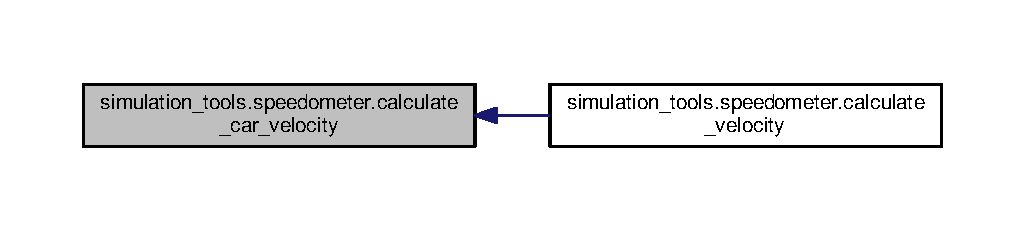
\includegraphics[width=350pt]{namespacesimulation__tools_1_1speedometer_a3323b9f8885fc1ce38dd75f2555cccba_icgraph}
\end{center}
\end{figure}


\index{simulation\+\_\+tools\+::speedometer@{simulation\+\_\+tools\+::speedometer}!calculate\+\_\+velocity@{calculate\+\_\+velocity}}
\index{calculate\+\_\+velocity@{calculate\+\_\+velocity}!simulation\+\_\+tools\+::speedometer@{simulation\+\_\+tools\+::speedometer}}
\subsubsection[{\texorpdfstring{calculate\+\_\+velocity(event)}{calculate_velocity(event)}}]{\setlength{\rightskip}{0pt plus 5cm}def simulation\+\_\+tools.\+speedometer.\+calculate\+\_\+velocity (
\begin{DoxyParamCaption}
\item[{}]{event}
\end{DoxyParamCaption}
)}\hypertarget{namespacesimulation__tools_1_1speedometer_aad7d50b1f509c29bb6b854ea4b649947}{}\label{namespacesimulation__tools_1_1speedometer_aad7d50b1f509c29bb6b854ea4b649947}


Definition at line 81 of file speedometer.\+py.



Here is the call graph for this function\+:
\nopagebreak
\begin{figure}[H]
\begin{center}
\leavevmode
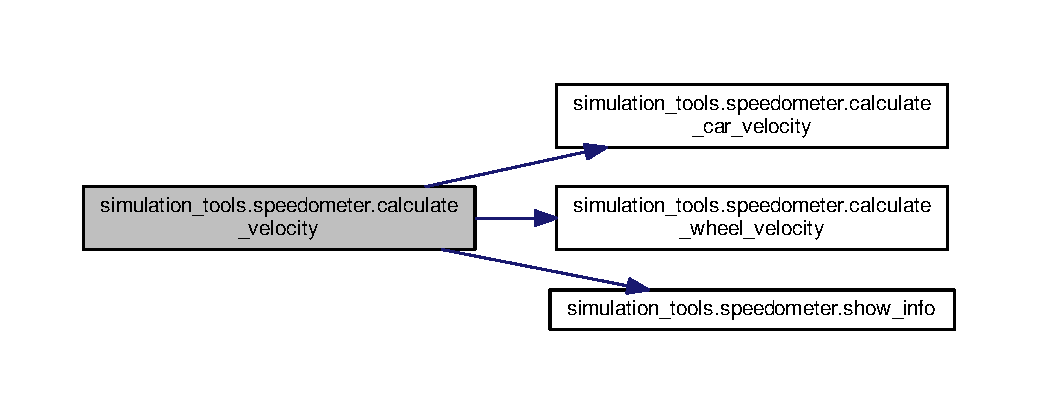
\includegraphics[width=350pt]{namespacesimulation__tools_1_1speedometer_aad7d50b1f509c29bb6b854ea4b649947_cgraph}
\end{center}
\end{figure}


\index{simulation\+\_\+tools\+::speedometer@{simulation\+\_\+tools\+::speedometer}!calculate\+\_\+wheel\+\_\+velocity@{calculate\+\_\+wheel\+\_\+velocity}}
\index{calculate\+\_\+wheel\+\_\+velocity@{calculate\+\_\+wheel\+\_\+velocity}!simulation\+\_\+tools\+::speedometer@{simulation\+\_\+tools\+::speedometer}}
\subsubsection[{\texorpdfstring{calculate\+\_\+wheel\+\_\+velocity()}{calculate_wheel_velocity()}}]{\setlength{\rightskip}{0pt plus 5cm}def simulation\+\_\+tools.\+speedometer.\+calculate\+\_\+wheel\+\_\+velocity (
\begin{DoxyParamCaption}
{}
\end{DoxyParamCaption}
)}\hypertarget{namespacesimulation__tools_1_1speedometer_af7706082fba920fe977bdb0e4dd464f8}{}\label{namespacesimulation__tools_1_1speedometer_af7706082fba920fe977bdb0e4dd464f8}


Definition at line 44 of file speedometer.\+py.



Here is the caller graph for this function\+:
\nopagebreak
\begin{figure}[H]
\begin{center}
\leavevmode
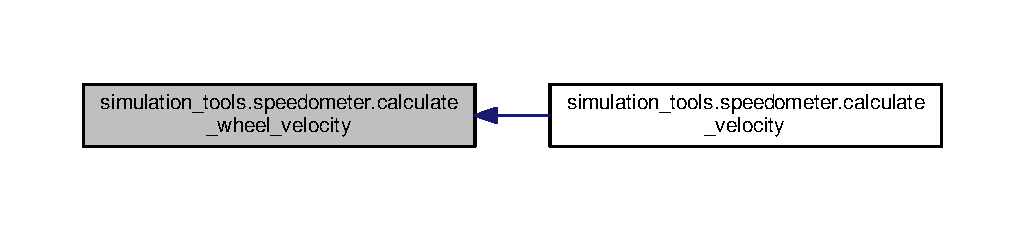
\includegraphics[width=350pt]{namespacesimulation__tools_1_1speedometer_af7706082fba920fe977bdb0e4dd464f8_icgraph}
\end{center}
\end{figure}


\index{simulation\+\_\+tools\+::speedometer@{simulation\+\_\+tools\+::speedometer}!link\+\_\+state\+\_\+callback@{link\+\_\+state\+\_\+callback}}
\index{link\+\_\+state\+\_\+callback@{link\+\_\+state\+\_\+callback}!simulation\+\_\+tools\+::speedometer@{simulation\+\_\+tools\+::speedometer}}
\subsubsection[{\texorpdfstring{link\+\_\+state\+\_\+callback(message)}{link_state_callback(message)}}]{\setlength{\rightskip}{0pt plus 5cm}def simulation\+\_\+tools.\+speedometer.\+link\+\_\+state\+\_\+callback (
\begin{DoxyParamCaption}
\item[{}]{message}
\end{DoxyParamCaption}
)}\hypertarget{namespacesimulation__tools_1_1speedometer_a9f675598deb566912ae5dfcef851ee8e}{}\label{namespacesimulation__tools_1_1speedometer_a9f675598deb566912ae5dfcef851ee8e}


Definition at line 21 of file speedometer.\+py.

\index{simulation\+\_\+tools\+::speedometer@{simulation\+\_\+tools\+::speedometer}!model\+\_\+state\+\_\+callback@{model\+\_\+state\+\_\+callback}}
\index{model\+\_\+state\+\_\+callback@{model\+\_\+state\+\_\+callback}!simulation\+\_\+tools\+::speedometer@{simulation\+\_\+tools\+::speedometer}}
\subsubsection[{\texorpdfstring{model\+\_\+state\+\_\+callback(message)}{model_state_callback(message)}}]{\setlength{\rightskip}{0pt plus 5cm}def simulation\+\_\+tools.\+speedometer.\+model\+\_\+state\+\_\+callback (
\begin{DoxyParamCaption}
\item[{}]{message}
\end{DoxyParamCaption}
)}\hypertarget{namespacesimulation__tools_1_1speedometer_ad8cbde404030a049eb657fd78f8bec45}{}\label{namespacesimulation__tools_1_1speedometer_ad8cbde404030a049eb657fd78f8bec45}


Definition at line 16 of file speedometer.\+py.

\index{simulation\+\_\+tools\+::speedometer@{simulation\+\_\+tools\+::speedometer}!show\+\_\+info@{show\+\_\+info}}
\index{show\+\_\+info@{show\+\_\+info}!simulation\+\_\+tools\+::speedometer@{simulation\+\_\+tools\+::speedometer}}
\subsubsection[{\texorpdfstring{show\+\_\+info()}{show_info()}}]{\setlength{\rightskip}{0pt plus 5cm}def simulation\+\_\+tools.\+speedometer.\+show\+\_\+info (
\begin{DoxyParamCaption}
{}
\end{DoxyParamCaption}
)}\hypertarget{namespacesimulation__tools_1_1speedometer_a605162cce10e81643f8f38ad72363b65}{}\label{namespacesimulation__tools_1_1speedometer_a605162cce10e81643f8f38ad72363b65}


Definition at line 55 of file speedometer.\+py.



Here is the caller graph for this function\+:
\nopagebreak
\begin{figure}[H]
\begin{center}
\leavevmode
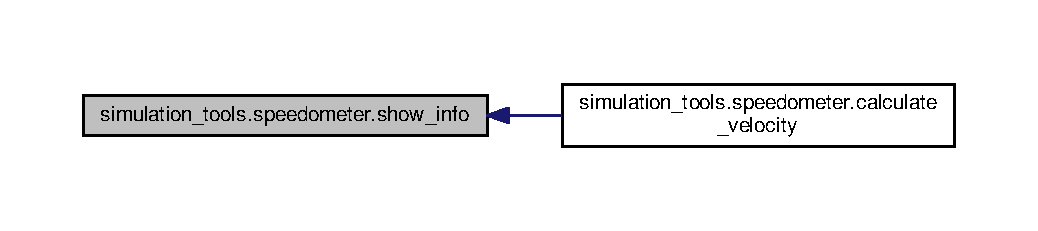
\includegraphics[width=350pt]{namespacesimulation__tools_1_1speedometer_a605162cce10e81643f8f38ad72363b65_icgraph}
\end{center}
\end{figure}




\subsection{Variable Documentation}
\index{simulation\+\_\+tools\+::speedometer@{simulation\+\_\+tools\+::speedometer}!car\+\_\+velocity@{car\+\_\+velocity}}
\index{car\+\_\+velocity@{car\+\_\+velocity}!simulation\+\_\+tools\+::speedometer@{simulation\+\_\+tools\+::speedometer}}
\subsubsection[{\texorpdfstring{car\+\_\+velocity}{car_velocity}}]{\setlength{\rightskip}{0pt plus 5cm}simulation\+\_\+tools.\+speedometer.\+car\+\_\+velocity = None}\hypertarget{namespacesimulation__tools_1_1speedometer_a58c9137e8b8cf3668ebac7ca01fa1bc9}{}\label{namespacesimulation__tools_1_1speedometer_a58c9137e8b8cf3668ebac7ca01fa1bc9}


Definition at line 9 of file speedometer.\+py.

\index{simulation\+\_\+tools\+::speedometer@{simulation\+\_\+tools\+::speedometer}!idle@{idle}}
\index{idle@{idle}!simulation\+\_\+tools\+::speedometer@{simulation\+\_\+tools\+::speedometer}}
\subsubsection[{\texorpdfstring{idle}{idle}}]{\setlength{\rightskip}{0pt plus 5cm}bool simulation\+\_\+tools.\+speedometer.\+idle = True}\hypertarget{namespacesimulation__tools_1_1speedometer_a7cadcb55f200a548ddc3de34bf4792e1}{}\label{namespacesimulation__tools_1_1speedometer_a7cadcb55f200a548ddc3de34bf4792e1}


Definition at line 78 of file speedometer.\+py.

\index{simulation\+\_\+tools\+::speedometer@{simulation\+\_\+tools\+::speedometer}!L\+I\+N\+K\+\_\+\+N\+A\+M\+ES@{L\+I\+N\+K\+\_\+\+N\+A\+M\+ES}}
\index{L\+I\+N\+K\+\_\+\+N\+A\+M\+ES@{L\+I\+N\+K\+\_\+\+N\+A\+M\+ES}!simulation\+\_\+tools\+::speedometer@{simulation\+\_\+tools\+::speedometer}}
\subsubsection[{\texorpdfstring{L\+I\+N\+K\+\_\+\+N\+A\+M\+ES}{LINK_NAMES}}]{\setlength{\rightskip}{0pt plus 5cm}list simulation\+\_\+tools.\+speedometer.\+L\+I\+N\+K\+\_\+\+N\+A\+M\+ES}\hypertarget{namespacesimulation__tools_1_1speedometer_a814c56b4196e3629a065df33256daab8}{}\label{namespacesimulation__tools_1_1speedometer_a814c56b4196e3629a065df33256daab8}
{\bfseries Initial value\+:}
\begin{DoxyCode}
1 = [
2     \textcolor{stringliteral}{'racer::left\_wheel\_front'},
3     \textcolor{stringliteral}{'racer::left\_wheel\_back'},
4     \textcolor{stringliteral}{'racer::right\_wheel\_front'},
5     \textcolor{stringliteral}{'racer::right\_wheel\_back'}]
\end{DoxyCode}


Definition at line 36 of file speedometer.\+py.

\index{simulation\+\_\+tools\+::speedometer@{simulation\+\_\+tools\+::speedometer}!link\+\_\+states\+\_\+message@{link\+\_\+states\+\_\+message}}
\index{link\+\_\+states\+\_\+message@{link\+\_\+states\+\_\+message}!simulation\+\_\+tools\+::speedometer@{simulation\+\_\+tools\+::speedometer}}
\subsubsection[{\texorpdfstring{link\+\_\+states\+\_\+message}{link_states_message}}]{\setlength{\rightskip}{0pt plus 5cm}simulation\+\_\+tools.\+speedometer.\+link\+\_\+states\+\_\+message = None}\hypertarget{namespacesimulation__tools_1_1speedometer_a57927328521dd9b5723725e98c92ab78}{}\label{namespacesimulation__tools_1_1speedometer_a57927328521dd9b5723725e98c92ab78}


Definition at line 13 of file speedometer.\+py.

\index{simulation\+\_\+tools\+::speedometer@{simulation\+\_\+tools\+::speedometer}!max\+\_\+car\+\_\+velocity@{max\+\_\+car\+\_\+velocity}}
\index{max\+\_\+car\+\_\+velocity@{max\+\_\+car\+\_\+velocity}!simulation\+\_\+tools\+::speedometer@{simulation\+\_\+tools\+::speedometer}}
\subsubsection[{\texorpdfstring{max\+\_\+car\+\_\+velocity}{max_car_velocity}}]{\setlength{\rightskip}{0pt plus 5cm}int simulation\+\_\+tools.\+speedometer.\+max\+\_\+car\+\_\+velocity = 0}\hypertarget{namespacesimulation__tools_1_1speedometer_a4db24fad416ca0a52b89d1529e4c38e9}{}\label{namespacesimulation__tools_1_1speedometer_a4db24fad416ca0a52b89d1529e4c38e9}


Definition at line 10 of file speedometer.\+py.

\index{simulation\+\_\+tools\+::speedometer@{simulation\+\_\+tools\+::speedometer}!model\+\_\+states\+\_\+message@{model\+\_\+states\+\_\+message}}
\index{model\+\_\+states\+\_\+message@{model\+\_\+states\+\_\+message}!simulation\+\_\+tools\+::speedometer@{simulation\+\_\+tools\+::speedometer}}
\subsubsection[{\texorpdfstring{model\+\_\+states\+\_\+message}{model_states_message}}]{\setlength{\rightskip}{0pt plus 5cm}simulation\+\_\+tools.\+speedometer.\+model\+\_\+states\+\_\+message = None}\hypertarget{namespacesimulation__tools_1_1speedometer_acd7f0f18f37f468db40dae82775a6313}{}\label{namespacesimulation__tools_1_1speedometer_acd7f0f18f37f468db40dae82775a6313}


Definition at line 12 of file speedometer.\+py.

\index{simulation\+\_\+tools\+::speedometer@{simulation\+\_\+tools\+::speedometer}!W\+H\+E\+E\+L\+\_\+\+R\+A\+D\+I\+US@{W\+H\+E\+E\+L\+\_\+\+R\+A\+D\+I\+US}}
\index{W\+H\+E\+E\+L\+\_\+\+R\+A\+D\+I\+US@{W\+H\+E\+E\+L\+\_\+\+R\+A\+D\+I\+US}!simulation\+\_\+tools\+::speedometer@{simulation\+\_\+tools\+::speedometer}}
\subsubsection[{\texorpdfstring{W\+H\+E\+E\+L\+\_\+\+R\+A\+D\+I\+US}{WHEEL_RADIUS}}]{\setlength{\rightskip}{0pt plus 5cm}float simulation\+\_\+tools.\+speedometer.\+W\+H\+E\+E\+L\+\_\+\+R\+A\+D\+I\+US = 0.\+05}\hypertarget{namespacesimulation__tools_1_1speedometer_abc578ddedab907737091cb86856732e7}{}\label{namespacesimulation__tools_1_1speedometer_abc578ddedab907737091cb86856732e7}


Definition at line 41 of file speedometer.\+py.

\index{simulation\+\_\+tools\+::speedometer@{simulation\+\_\+tools\+::speedometer}!wheel\+\_\+velocity@{wheel\+\_\+velocity}}
\index{wheel\+\_\+velocity@{wheel\+\_\+velocity}!simulation\+\_\+tools\+::speedometer@{simulation\+\_\+tools\+::speedometer}}
\subsubsection[{\texorpdfstring{wheel\+\_\+velocity}{wheel_velocity}}]{\setlength{\rightskip}{0pt plus 5cm}simulation\+\_\+tools.\+speedometer.\+wheel\+\_\+velocity = None}\hypertarget{namespacesimulation__tools_1_1speedometer_a6d93deddfe3b707f9be21ed85278d8b5}{}\label{namespacesimulation__tools_1_1speedometer_a6d93deddfe3b707f9be21ed85278d8b5}


Definition at line 8 of file speedometer.\+py.


\hypertarget{namespacesimulation__tools_1_1track}{}\section{simulation\+\_\+tools.\+track Namespace Reference}
\label{namespacesimulation__tools_1_1track}\index{simulation\+\_\+tools.\+track@{simulation\+\_\+tools.\+track}}
\subsection*{Classes}
\begin{DoxyCompactItemize}
\item 
class \hyperlink{classsimulation__tools_1_1track_1_1_track}{Track}
\item 
class \hyperlink{classsimulation__tools_1_1track_1_1_track_position}{Track\+Position}
\end{DoxyCompactItemize}
\subsection*{Variables}
\begin{DoxyCompactItemize}
\item 
\hyperlink{namespacesimulation__tools_1_1track_a927c1793846ca41f328e4b427075cafd}{Point} = namedtuple(\char`\"{}Point\char`\"{}, \mbox{[}\char`\"{}x\char`\"{}, \char`\"{}y\char`\"{}\mbox{]})
\item 
\hyperlink{namespacesimulation__tools_1_1track_ab9ddc4d3ba8bb81a3ce02320f46c8a55}{P\+O\+I\+N\+TS}
\item 
\hyperlink{namespacesimulation__tools_1_1track_ac731095c2502c445d46302406cb81651}{track} = \hyperlink{classsimulation__tools_1_1track_1_1_track}{Track}(\hyperlink{namespacesimulation__tools_1_1track_ab9ddc4d3ba8bb81a3ce02320f46c8a55}{P\+O\+I\+N\+TS})
\end{DoxyCompactItemize}


\subsection{Variable Documentation}
\index{simulation\+\_\+tools\+::track@{simulation\+\_\+tools\+::track}!Point@{Point}}
\index{Point@{Point}!simulation\+\_\+tools\+::track@{simulation\+\_\+tools\+::track}}
\subsubsection[{\texorpdfstring{Point}{Point}}]{\setlength{\rightskip}{0pt plus 5cm}simulation\+\_\+tools.\+track.\+Point = namedtuple(\char`\"{}Point\char`\"{}, \mbox{[}\char`\"{}x\char`\"{}, \char`\"{}y\char`\"{}\mbox{]})}\hypertarget{namespacesimulation__tools_1_1track_a927c1793846ca41f328e4b427075cafd}{}\label{namespacesimulation__tools_1_1track_a927c1793846ca41f328e4b427075cafd}


Definition at line 10 of file track.\+py.

\index{simulation\+\_\+tools\+::track@{simulation\+\_\+tools\+::track}!P\+O\+I\+N\+TS@{P\+O\+I\+N\+TS}}
\index{P\+O\+I\+N\+TS@{P\+O\+I\+N\+TS}!simulation\+\_\+tools\+::track@{simulation\+\_\+tools\+::track}}
\subsubsection[{\texorpdfstring{P\+O\+I\+N\+TS}{POINTS}}]{\setlength{\rightskip}{0pt plus 5cm}simulation\+\_\+tools.\+track.\+P\+O\+I\+N\+TS}\hypertarget{namespacesimulation__tools_1_1track_ab9ddc4d3ba8bb81a3ce02320f46c8a55}{}\label{namespacesimulation__tools_1_1track_ab9ddc4d3ba8bb81a3ce02320f46c8a55}


Definition at line 85 of file track.\+py.

\index{simulation\+\_\+tools\+::track@{simulation\+\_\+tools\+::track}!track@{track}}
\index{track@{track}!simulation\+\_\+tools\+::track@{simulation\+\_\+tools\+::track}}
\subsubsection[{\texorpdfstring{track}{track}}]{\setlength{\rightskip}{0pt plus 5cm}simulation\+\_\+tools.\+track.\+track = {\bf Track}({\bf P\+O\+I\+N\+TS})}\hypertarget{namespacesimulation__tools_1_1track_ac731095c2502c445d46302406cb81651}{}\label{namespacesimulation__tools_1_1track_ac731095c2502c445d46302406cb81651}


Definition at line 137 of file track.\+py.


\hypertarget{namespacetrain}{}\section{train Namespace Reference}
\label{namespacetrain}\index{train@{train}}
\subsection*{Classes}
\begin{DoxyCompactItemize}
\item 
class \hyperlink{classtrain_1_1_training_node}{Training\+Node}
\end{DoxyCompactItemize}
\subsection*{Variables}
\begin{DoxyCompactItemize}
\item 
int \hyperlink{namespacetrain_ad27ad66c4ffaa353cbb94c83a7968ce9}{M\+A\+X\+\_\+\+E\+P\+I\+S\+O\+D\+E\+\_\+\+L\+E\+N\+G\+TH} = 5000
\item 
int \hyperlink{namespacetrain_a4e23f5a2db715f6c10039c5ab27d4f44}{I\+N\+I\+T\+I\+A\+L\+\_\+\+R\+A\+N\+D\+O\+M\+\_\+\+P\+O\+P\+U\+L\+A\+T\+I\+O\+N\+\_\+\+S\+I\+ZE} = 250
\item 
bool \hyperlink{namespacetrain_ace8c65d5c0d8f68ac961d3a2bf198e5d}{C\+O\+N\+T\+I\+N\+U\+E\+\_\+\+T\+R\+A\+I\+N\+I\+NG} = True
\item 
\hyperlink{namespacetrain_a7c68a6981d3c74c76920e856fc7c2419}{node} = \hyperlink{classtrain_1_1_training_node}{Training\+Node}()
\end{DoxyCompactItemize}


\subsection{Variable Documentation}
\index{train@{train}!C\+O\+N\+T\+I\+N\+U\+E\+\_\+\+T\+R\+A\+I\+N\+I\+NG@{C\+O\+N\+T\+I\+N\+U\+E\+\_\+\+T\+R\+A\+I\+N\+I\+NG}}
\index{C\+O\+N\+T\+I\+N\+U\+E\+\_\+\+T\+R\+A\+I\+N\+I\+NG@{C\+O\+N\+T\+I\+N\+U\+E\+\_\+\+T\+R\+A\+I\+N\+I\+NG}!train@{train}}
\subsubsection[{\texorpdfstring{C\+O\+N\+T\+I\+N\+U\+E\+\_\+\+T\+R\+A\+I\+N\+I\+NG}{CONTINUE_TRAINING}}]{\setlength{\rightskip}{0pt plus 5cm}bool train.\+C\+O\+N\+T\+I\+N\+U\+E\+\_\+\+T\+R\+A\+I\+N\+I\+NG = True}\hypertarget{namespacetrain_ace8c65d5c0d8f68ac961d3a2bf198e5d}{}\label{namespacetrain_ace8c65d5c0d8f68ac961d3a2bf198e5d}


Definition at line 15 of file train.\+py.

\index{train@{train}!I\+N\+I\+T\+I\+A\+L\+\_\+\+R\+A\+N\+D\+O\+M\+\_\+\+P\+O\+P\+U\+L\+A\+T\+I\+O\+N\+\_\+\+S\+I\+ZE@{I\+N\+I\+T\+I\+A\+L\+\_\+\+R\+A\+N\+D\+O\+M\+\_\+\+P\+O\+P\+U\+L\+A\+T\+I\+O\+N\+\_\+\+S\+I\+ZE}}
\index{I\+N\+I\+T\+I\+A\+L\+\_\+\+R\+A\+N\+D\+O\+M\+\_\+\+P\+O\+P\+U\+L\+A\+T\+I\+O\+N\+\_\+\+S\+I\+ZE@{I\+N\+I\+T\+I\+A\+L\+\_\+\+R\+A\+N\+D\+O\+M\+\_\+\+P\+O\+P\+U\+L\+A\+T\+I\+O\+N\+\_\+\+S\+I\+ZE}!train@{train}}
\subsubsection[{\texorpdfstring{I\+N\+I\+T\+I\+A\+L\+\_\+\+R\+A\+N\+D\+O\+M\+\_\+\+P\+O\+P\+U\+L\+A\+T\+I\+O\+N\+\_\+\+S\+I\+ZE}{INITIAL_RANDOM_POPULATION_SIZE}}]{\setlength{\rightskip}{0pt plus 5cm}int train.\+I\+N\+I\+T\+I\+A\+L\+\_\+\+R\+A\+N\+D\+O\+M\+\_\+\+P\+O\+P\+U\+L\+A\+T\+I\+O\+N\+\_\+\+S\+I\+ZE = 250}\hypertarget{namespacetrain_a4e23f5a2db715f6c10039c5ab27d4f44}{}\label{namespacetrain_a4e23f5a2db715f6c10039c5ab27d4f44}


Definition at line 14 of file train.\+py.

\index{train@{train}!M\+A\+X\+\_\+\+E\+P\+I\+S\+O\+D\+E\+\_\+\+L\+E\+N\+G\+TH@{M\+A\+X\+\_\+\+E\+P\+I\+S\+O\+D\+E\+\_\+\+L\+E\+N\+G\+TH}}
\index{M\+A\+X\+\_\+\+E\+P\+I\+S\+O\+D\+E\+\_\+\+L\+E\+N\+G\+TH@{M\+A\+X\+\_\+\+E\+P\+I\+S\+O\+D\+E\+\_\+\+L\+E\+N\+G\+TH}!train@{train}}
\subsubsection[{\texorpdfstring{M\+A\+X\+\_\+\+E\+P\+I\+S\+O\+D\+E\+\_\+\+L\+E\+N\+G\+TH}{MAX_EPISODE_LENGTH}}]{\setlength{\rightskip}{0pt plus 5cm}int train.\+M\+A\+X\+\_\+\+E\+P\+I\+S\+O\+D\+E\+\_\+\+L\+E\+N\+G\+TH = 5000}\hypertarget{namespacetrain_ad27ad66c4ffaa353cbb94c83a7968ce9}{}\label{namespacetrain_ad27ad66c4ffaa353cbb94c83a7968ce9}


Definition at line 13 of file train.\+py.

\index{train@{train}!node@{node}}
\index{node@{node}!train@{train}}
\subsubsection[{\texorpdfstring{node}{node}}]{\setlength{\rightskip}{0pt plus 5cm}train.\+node = {\bf Training\+Node}()}\hypertarget{namespacetrain_a7c68a6981d3c74c76920e856fc7c2419}{}\label{namespacetrain_a7c68a6981d3c74c76920e856fc7c2419}


Definition at line 99 of file train.\+py.


\hypertarget{namespacewallfollowing}{}\section{wallfollowing Namespace Reference}
\label{namespacewallfollowing}\index{wallfollowing@{wallfollowing}}
\subsection*{Classes}
\begin{DoxyCompactItemize}
\item 
class \hyperlink{classwallfollowing_1_1_parameters}{Parameters}
\item 
class \hyperlink{classwallfollowing_1_1_p_i_d_controller}{P\+I\+D\+Controller}
\end{DoxyCompactItemize}
\subsection*{Functions}
\begin{DoxyCompactItemize}
\item 
def \hyperlink{namespacewallfollowing_a908b60b64e20dec7078e707a829b610d}{map} (in\+\_\+lower, in\+\_\+upper, out\+\_\+lower, out\+\_\+upper, value)
\item 
def \hyperlink{namespacewallfollowing_a66b98adda1f5c1ba1ed6c0029a5d27f6}{drive} (angle, velocity)
\item 
def \hyperlink{namespacewallfollowing_aacb7060aae10ef40bdacceb57283943c}{get\+\_\+scan\+\_\+as\+\_\+cartesian} (laser\+\_\+scan)
\item 
def \hyperlink{namespacewallfollowing_a85455c82dd12c297c8cbc3227c1ba598}{find\+\_\+left\+\_\+right\+\_\+border} (points, margin\+\_\+relative=0.\+1)
\item 
def \hyperlink{namespacewallfollowing_ae4edc6135d6c1a9b38674119a96b3375}{follow\+\_\+walls} (left\+\_\+circle, right\+\_\+circle, barrier, delta\+\_\+time)
\item 
def \hyperlink{namespacewallfollowing_a48cc636bf9056c7b7b2db2dede94474a}{handle\+\_\+scan} (laser\+\_\+scan, delta\+\_\+time)
\item 
def \hyperlink{namespacewallfollowing_a53e20aefe2b925b41b17f60b6673840b}{laser\+\_\+callback} (scan\+\_\+message)
\item 
def \hyperlink{namespacewallfollowing_aa82241200b0cac397334403b54a2c1ad}{dynamic\+\_\+configuration\+\_\+callback} (config, level)
\end{DoxyCompactItemize}
\subsection*{Variables}
\begin{DoxyCompactItemize}
\item 
string \hyperlink{namespacewallfollowing_a765ce45df7d0c3d9134fc83534029e36}{T\+O\+P\+I\+C\+\_\+\+D\+R\+I\+V\+E\+\_\+\+P\+A\+R\+A\+M\+E\+T\+E\+RS} = \char`\"{}/input/drive\+\_\+param/autonomous\char`\"{}
\item 
string \hyperlink{namespacewallfollowing_a7e38e617465ebdfa7ec0576ac63443f8}{T\+O\+P\+I\+C\+\_\+\+L\+A\+S\+E\+R\+\_\+\+S\+C\+AN} = \char`\"{}/scan\char`\"{}
\item 
int \hyperlink{namespacewallfollowing_a9ee8d77a4629b5d8ecb2899da6e3a7fe}{last\+\_\+speed} = 0
\item 
dictionary \hyperlink{namespacewallfollowing_ac161be1e11f04000d35ca725afa3ccdf}{D\+E\+F\+A\+U\+L\+T\+\_\+\+P\+A\+R\+A\+M\+E\+T\+E\+RS}
\item 
\hyperlink{namespacewallfollowing_ab6c7c8e53e8b1cd44872666515dd5764}{last\+\_\+scan} = None
\item 
\hyperlink{namespacewallfollowing_ae96254db0e391eed9862d0a6f636033e}{parameters} = \hyperlink{classwallfollowing_1_1_parameters}{Parameters}(\hyperlink{namespacewallfollowing_ac161be1e11f04000d35ca725afa3ccdf}{D\+E\+F\+A\+U\+L\+T\+\_\+\+P\+A\+R\+A\+M\+E\+T\+E\+RS})
\item 
\hyperlink{namespacewallfollowing_adc9f95e0b626be8ddae98a596a38e7e8}{pid}
\item 
\hyperlink{namespacewallfollowing_aa69138defbbc5f21e99db50a6b3c903f}{drive\+\_\+parameters\+\_\+publisher}
\end{DoxyCompactItemize}


\subsection{Function Documentation}
\index{wallfollowing@{wallfollowing}!drive@{drive}}
\index{drive@{drive}!wallfollowing@{wallfollowing}}
\subsubsection[{\texorpdfstring{drive(angle, velocity)}{drive(angle, velocity)}}]{\setlength{\rightskip}{0pt plus 5cm}def wallfollowing.\+drive (
\begin{DoxyParamCaption}
\item[{}]{angle, }
\item[{}]{velocity}
\end{DoxyParamCaption}
)}\hypertarget{namespacewallfollowing_a66b98adda1f5c1ba1ed6c0029a5d27f6}{}\label{namespacewallfollowing_a66b98adda1f5c1ba1ed6c0029a5d27f6}


Definition at line 98 of file wallfollowing.\+py.

\index{wallfollowing@{wallfollowing}!dynamic\+\_\+configuration\+\_\+callback@{dynamic\+\_\+configuration\+\_\+callback}}
\index{dynamic\+\_\+configuration\+\_\+callback@{dynamic\+\_\+configuration\+\_\+callback}!wallfollowing@{wallfollowing}}
\subsubsection[{\texorpdfstring{dynamic\+\_\+configuration\+\_\+callback(config, level)}{dynamic_configuration_callback(config, level)}}]{\setlength{\rightskip}{0pt plus 5cm}def wallfollowing.\+dynamic\+\_\+configuration\+\_\+callback (
\begin{DoxyParamCaption}
\item[{}]{config, }
\item[{}]{level}
\end{DoxyParamCaption}
)}\hypertarget{namespacewallfollowing_aa82241200b0cac397334403b54a2c1ad}{}\label{namespacewallfollowing_aa82241200b0cac397334403b54a2c1ad}


Definition at line 221 of file wallfollowing.\+py.

\index{wallfollowing@{wallfollowing}!find\+\_\+left\+\_\+right\+\_\+border@{find\+\_\+left\+\_\+right\+\_\+border}}
\index{find\+\_\+left\+\_\+right\+\_\+border@{find\+\_\+left\+\_\+right\+\_\+border}!wallfollowing@{wallfollowing}}
\subsubsection[{\texorpdfstring{find\+\_\+left\+\_\+right\+\_\+border(points, margin\+\_\+relative=0.\+1)}{find_left_right_border(points, margin_relative=0.1)}}]{\setlength{\rightskip}{0pt plus 5cm}def wallfollowing.\+find\+\_\+left\+\_\+right\+\_\+border (
\begin{DoxyParamCaption}
\item[{}]{points, }
\item[{}]{margin\+\_\+relative = {\ttfamily 0.1}}
\end{DoxyParamCaption}
)}\hypertarget{namespacewallfollowing_a85455c82dd12c297c8cbc3227c1ba598}{}\label{namespacewallfollowing_a85455c82dd12c297c8cbc3227c1ba598}


Definition at line 124 of file wallfollowing.\+py.



Here is the caller graph for this function\+:
\nopagebreak
\begin{figure}[H]
\begin{center}
\leavevmode
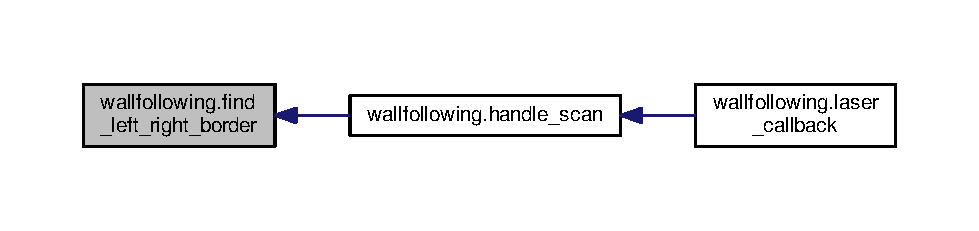
\includegraphics[width=350pt]{namespacewallfollowing_a85455c82dd12c297c8cbc3227c1ba598_icgraph}
\end{center}
\end{figure}


\index{wallfollowing@{wallfollowing}!follow\+\_\+walls@{follow\+\_\+walls}}
\index{follow\+\_\+walls@{follow\+\_\+walls}!wallfollowing@{wallfollowing}}
\subsubsection[{\texorpdfstring{follow\+\_\+walls(left\+\_\+circle, right\+\_\+circle, barrier, delta\+\_\+time)}{follow_walls(left_circle, right_circle, barrier, delta_time)}}]{\setlength{\rightskip}{0pt plus 5cm}def wallfollowing.\+follow\+\_\+walls (
\begin{DoxyParamCaption}
\item[{}]{left\+\_\+circle, }
\item[{}]{right\+\_\+circle, }
\item[{}]{barrier, }
\item[{}]{delta\+\_\+time}
\end{DoxyParamCaption}
)}\hypertarget{namespacewallfollowing_ae4edc6135d6c1a9b38674119a96b3375}{}\label{namespacewallfollowing_ae4edc6135d6c1a9b38674119a96b3375}


Definition at line 133 of file wallfollowing.\+py.



Here is the call graph for this function\+:
\nopagebreak
\begin{figure}[H]
\begin{center}
\leavevmode
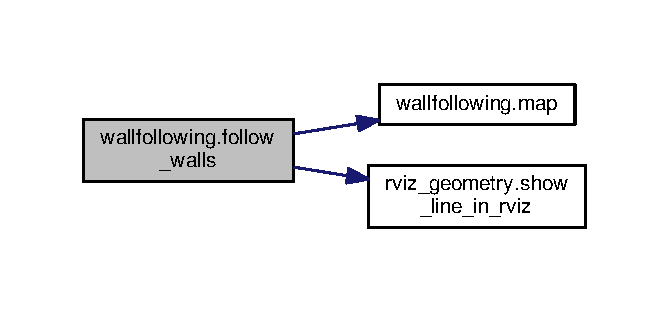
\includegraphics[width=321pt]{namespacewallfollowing_ae4edc6135d6c1a9b38674119a96b3375_cgraph}
\end{center}
\end{figure}




Here is the caller graph for this function\+:
\nopagebreak
\begin{figure}[H]
\begin{center}
\leavevmode
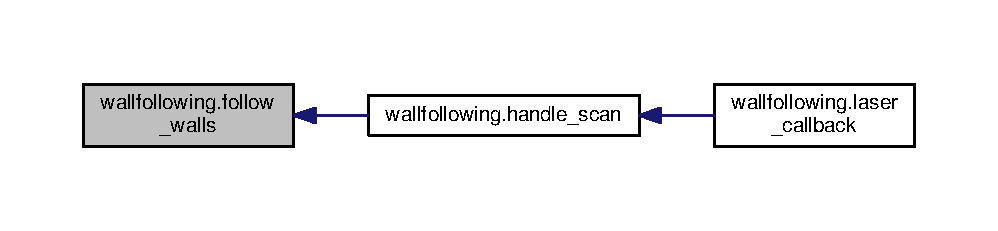
\includegraphics[width=350pt]{namespacewallfollowing_ae4edc6135d6c1a9b38674119a96b3375_icgraph}
\end{center}
\end{figure}


\index{wallfollowing@{wallfollowing}!get\+\_\+scan\+\_\+as\+\_\+cartesian@{get\+\_\+scan\+\_\+as\+\_\+cartesian}}
\index{get\+\_\+scan\+\_\+as\+\_\+cartesian@{get\+\_\+scan\+\_\+as\+\_\+cartesian}!wallfollowing@{wallfollowing}}
\subsubsection[{\texorpdfstring{get\+\_\+scan\+\_\+as\+\_\+cartesian(laser\+\_\+scan)}{get_scan_as_cartesian(laser_scan)}}]{\setlength{\rightskip}{0pt plus 5cm}def wallfollowing.\+get\+\_\+scan\+\_\+as\+\_\+cartesian (
\begin{DoxyParamCaption}
\item[{}]{laser\+\_\+scan}
\end{DoxyParamCaption}
)}\hypertarget{namespacewallfollowing_aacb7060aae10ef40bdacceb57283943c}{}\label{namespacewallfollowing_aacb7060aae10ef40bdacceb57283943c}


Definition at line 105 of file wallfollowing.\+py.



Here is the caller graph for this function\+:
\nopagebreak
\begin{figure}[H]
\begin{center}
\leavevmode
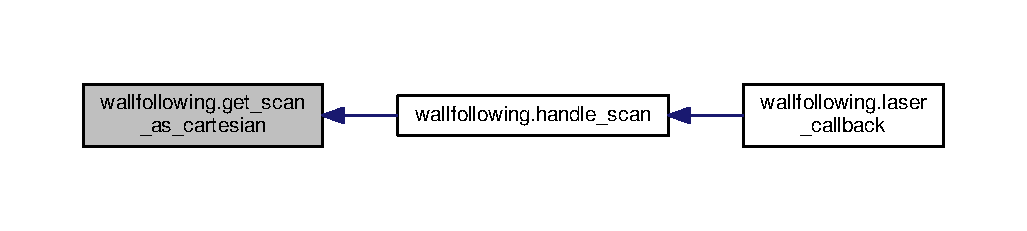
\includegraphics[width=350pt]{namespacewallfollowing_aacb7060aae10ef40bdacceb57283943c_icgraph}
\end{center}
\end{figure}


\index{wallfollowing@{wallfollowing}!handle\+\_\+scan@{handle\+\_\+scan}}
\index{handle\+\_\+scan@{handle\+\_\+scan}!wallfollowing@{wallfollowing}}
\subsubsection[{\texorpdfstring{handle\+\_\+scan(laser\+\_\+scan, delta\+\_\+time)}{handle_scan(laser_scan, delta_time)}}]{\setlength{\rightskip}{0pt plus 5cm}def wallfollowing.\+handle\+\_\+scan (
\begin{DoxyParamCaption}
\item[{}]{laser\+\_\+scan, }
\item[{}]{delta\+\_\+time}
\end{DoxyParamCaption}
)}\hypertarget{namespacewallfollowing_a48cc636bf9056c7b7b2db2dede94474a}{}\label{namespacewallfollowing_a48cc636bf9056c7b7b2db2dede94474a}


Definition at line 182 of file wallfollowing.\+py.



Here is the call graph for this function\+:
\nopagebreak
\begin{figure}[H]
\begin{center}
\leavevmode
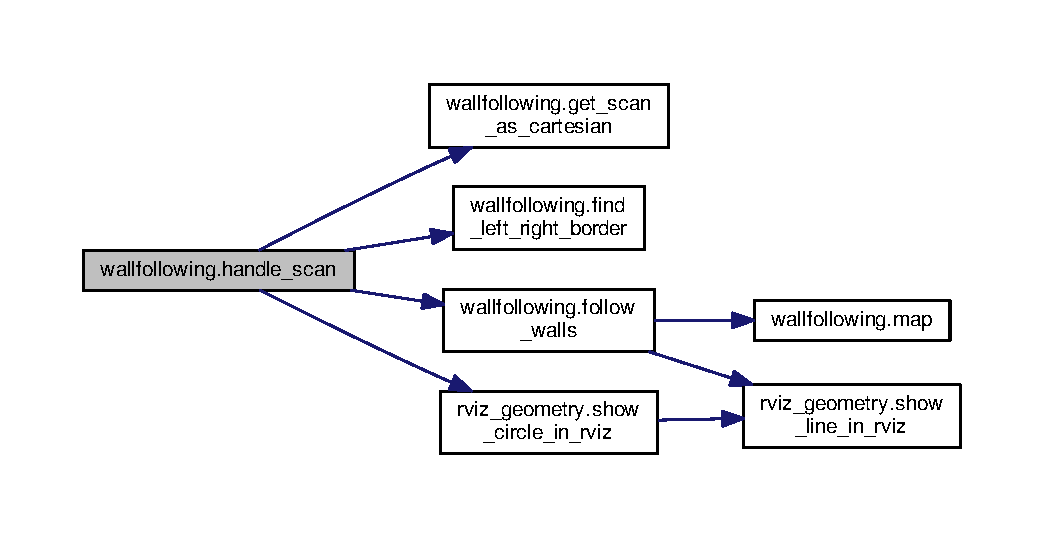
\includegraphics[width=350pt]{namespacewallfollowing_a48cc636bf9056c7b7b2db2dede94474a_cgraph}
\end{center}
\end{figure}




Here is the caller graph for this function\+:
\nopagebreak
\begin{figure}[H]
\begin{center}
\leavevmode
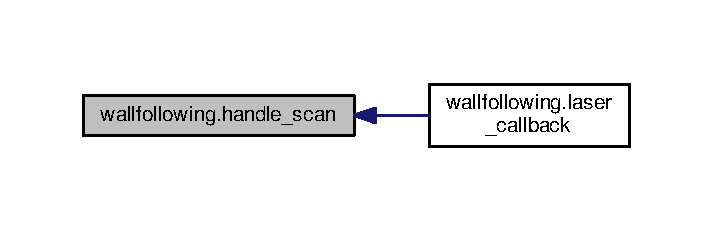
\includegraphics[width=342pt]{namespacewallfollowing_a48cc636bf9056c7b7b2db2dede94474a_icgraph}
\end{center}
\end{figure}


\index{wallfollowing@{wallfollowing}!laser\+\_\+callback@{laser\+\_\+callback}}
\index{laser\+\_\+callback@{laser\+\_\+callback}!wallfollowing@{wallfollowing}}
\subsubsection[{\texorpdfstring{laser\+\_\+callback(scan\+\_\+message)}{laser_callback(scan_message)}}]{\setlength{\rightskip}{0pt plus 5cm}def wallfollowing.\+laser\+\_\+callback (
\begin{DoxyParamCaption}
\item[{}]{scan\+\_\+message}
\end{DoxyParamCaption}
)}\hypertarget{namespacewallfollowing_a53e20aefe2b925b41b17f60b6673840b}{}\label{namespacewallfollowing_a53e20aefe2b925b41b17f60b6673840b}


Definition at line 210 of file wallfollowing.\+py.



Here is the call graph for this function\+:
\nopagebreak
\begin{figure}[H]
\begin{center}
\leavevmode
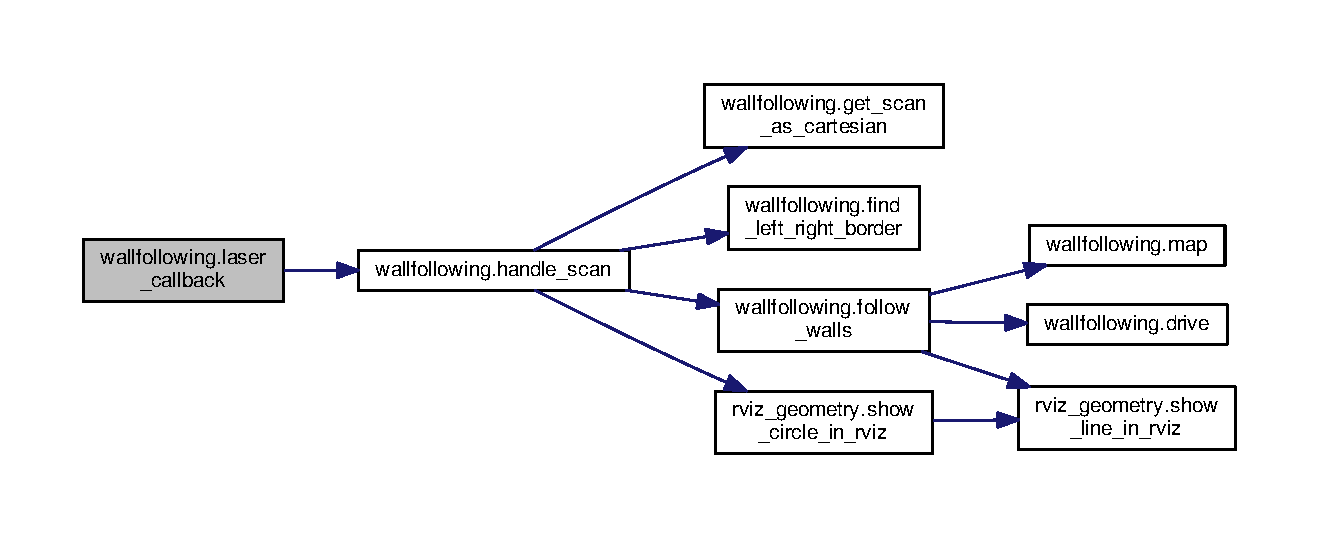
\includegraphics[width=350pt]{namespacewallfollowing_a53e20aefe2b925b41b17f60b6673840b_cgraph}
\end{center}
\end{figure}


\index{wallfollowing@{wallfollowing}!map@{map}}
\index{map@{map}!wallfollowing@{wallfollowing}}
\subsubsection[{\texorpdfstring{map(in\+\_\+lower, in\+\_\+upper, out\+\_\+lower, out\+\_\+upper, value)}{map(in_lower, in_upper, out_lower, out_upper, value)}}]{\setlength{\rightskip}{0pt plus 5cm}def wallfollowing.\+map (
\begin{DoxyParamCaption}
\item[{}]{in\+\_\+lower, }
\item[{}]{in\+\_\+upper, }
\item[{}]{out\+\_\+lower, }
\item[{}]{out\+\_\+upper, }
\item[{}]{value}
\end{DoxyParamCaption}
)}\hypertarget{namespacewallfollowing_a908b60b64e20dec7078e707a829b610d}{}\label{namespacewallfollowing_a908b60b64e20dec7078e707a829b610d}


Definition at line 92 of file wallfollowing.\+py.



Here is the caller graph for this function\+:
\nopagebreak
\begin{figure}[H]
\begin{center}
\leavevmode
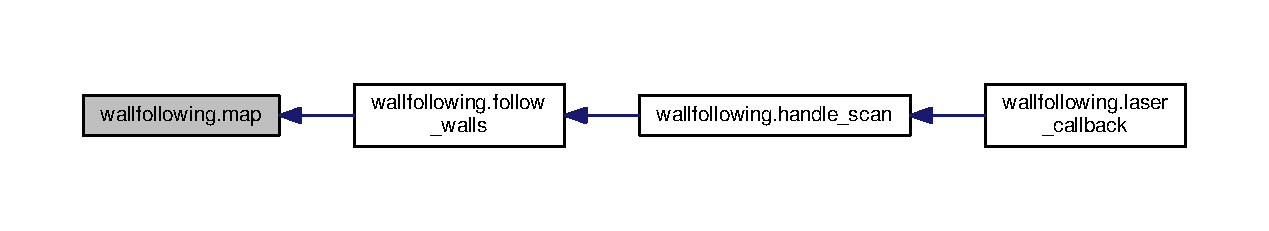
\includegraphics[width=350pt]{namespacewallfollowing_a908b60b64e20dec7078e707a829b610d_icgraph}
\end{center}
\end{figure}




\subsection{Variable Documentation}
\index{wallfollowing@{wallfollowing}!D\+E\+F\+A\+U\+L\+T\+\_\+\+P\+A\+R\+A\+M\+E\+T\+E\+RS@{D\+E\+F\+A\+U\+L\+T\+\_\+\+P\+A\+R\+A\+M\+E\+T\+E\+RS}}
\index{D\+E\+F\+A\+U\+L\+T\+\_\+\+P\+A\+R\+A\+M\+E\+T\+E\+RS@{D\+E\+F\+A\+U\+L\+T\+\_\+\+P\+A\+R\+A\+M\+E\+T\+E\+RS}!wallfollowing@{wallfollowing}}
\subsubsection[{\texorpdfstring{D\+E\+F\+A\+U\+L\+T\+\_\+\+P\+A\+R\+A\+M\+E\+T\+E\+RS}{DEFAULT_PARAMETERS}}]{\setlength{\rightskip}{0pt plus 5cm}dictionary wallfollowing.\+D\+E\+F\+A\+U\+L\+T\+\_\+\+P\+A\+R\+A\+M\+E\+T\+E\+RS}\hypertarget{namespacewallfollowing_ac161be1e11f04000d35ca725afa3ccdf}{}\label{namespacewallfollowing_ac161be1e11f04000d35ca725afa3ccdf}
{\bfseries Initial value\+:}
\begin{DoxyCode}
1 = \{
2     \textcolor{stringliteral}{'min\_throttle'}: 0.2,
3     \textcolor{stringliteral}{'max\_throttle'}: 1.0,
4 
5     \textcolor{stringliteral}{'radius\_lower'}: 2,
6     \textcolor{stringliteral}{'radius\_upper'}: 30,
7 
8     \textcolor{stringliteral}{'steering\_slow\_down'}: 4,
9     \textcolor{stringliteral}{'steering\_slow\_down\_dead\_zone'}: 0.2,
10 
11     \textcolor{stringliteral}{'high\_speed\_steering\_limit'}: 0.5,
12     \textcolor{stringliteral}{'high\_speed\_steering\_limit\_dead\_zone'}: 0.2,
13 
14     \textcolor{stringliteral}{'max\_acceleration'}: 0.4,
15 
16     \textcolor{stringliteral}{'corner\_cutting'}: 1.4,
17     \textcolor{stringliteral}{'straight\_smoothing'}: 1.0,
18 
19     \textcolor{stringliteral}{'barrier\_size\_realtive'}: 0.1,
20     \textcolor{stringliteral}{'barrier\_lower\_limit'}: 1,
21     \textcolor{stringliteral}{'barrier\_upper\_limit'}: 15,
22     \textcolor{stringliteral}{'barrier\_exponent'}: 1.4,
23 
24     \textcolor{stringliteral}{'controller\_p'}: 4,
25     \textcolor{stringliteral}{'controller\_i'}: 0.2,
26     \textcolor{stringliteral}{'controller\_d'}: 0.02
27 \}
\end{DoxyCode}


Definition at line 24 of file wallfollowing.\+py.

\index{wallfollowing@{wallfollowing}!drive\+\_\+parameters\+\_\+publisher@{drive\+\_\+parameters\+\_\+publisher}}
\index{drive\+\_\+parameters\+\_\+publisher@{drive\+\_\+parameters\+\_\+publisher}!wallfollowing@{wallfollowing}}
\subsubsection[{\texorpdfstring{drive\+\_\+parameters\+\_\+publisher}{drive_parameters_publisher}}]{\setlength{\rightskip}{0pt plus 5cm}wallfollowing.\+drive\+\_\+parameters\+\_\+publisher}\hypertarget{namespacewallfollowing_aa69138defbbc5f21e99db50a6b3c903f}{}\label{namespacewallfollowing_aa69138defbbc5f21e99db50a6b3c903f}
{\bfseries Initial value\+:}
\begin{DoxyCode}
1 = rospy.Publisher(
2     TOPIC\_DRIVE\_PARAMETERS, drive\_param, queue\_size=1)
\end{DoxyCode}


Definition at line 239 of file wallfollowing.\+py.

\index{wallfollowing@{wallfollowing}!last\+\_\+scan@{last\+\_\+scan}}
\index{last\+\_\+scan@{last\+\_\+scan}!wallfollowing@{wallfollowing}}
\subsubsection[{\texorpdfstring{last\+\_\+scan}{last_scan}}]{\setlength{\rightskip}{0pt plus 5cm}wallfollowing.\+last\+\_\+scan = None}\hypertarget{namespacewallfollowing_ab6c7c8e53e8b1cd44872666515dd5764}{}\label{namespacewallfollowing_ab6c7c8e53e8b1cd44872666515dd5764}


Definition at line 207 of file wallfollowing.\+py.

\index{wallfollowing@{wallfollowing}!last\+\_\+speed@{last\+\_\+speed}}
\index{last\+\_\+speed@{last\+\_\+speed}!wallfollowing@{wallfollowing}}
\subsubsection[{\texorpdfstring{last\+\_\+speed}{last_speed}}]{\setlength{\rightskip}{0pt plus 5cm}int wallfollowing.\+last\+\_\+speed = 0}\hypertarget{namespacewallfollowing_a9ee8d77a4629b5d8ecb2899da6e3a7fe}{}\label{namespacewallfollowing_a9ee8d77a4629b5d8ecb2899da6e3a7fe}


Definition at line 22 of file wallfollowing.\+py.

\index{wallfollowing@{wallfollowing}!parameters@{parameters}}
\index{parameters@{parameters}!wallfollowing@{wallfollowing}}
\subsubsection[{\texorpdfstring{parameters}{parameters}}]{\setlength{\rightskip}{0pt plus 5cm}wallfollowing.\+parameters = {\bf Parameters}({\bf D\+E\+F\+A\+U\+L\+T\+\_\+\+P\+A\+R\+A\+M\+E\+T\+E\+RS})}\hypertarget{namespacewallfollowing_ae96254db0e391eed9862d0a6f636033e}{}\label{namespacewallfollowing_ae96254db0e391eed9862d0a6f636033e}


Definition at line 231 of file wallfollowing.\+py.

\index{wallfollowing@{wallfollowing}!pid@{pid}}
\index{pid@{pid}!wallfollowing@{wallfollowing}}
\subsubsection[{\texorpdfstring{pid}{pid}}]{\setlength{\rightskip}{0pt plus 5cm}wallfollowing.\+pid}\hypertarget{namespacewallfollowing_adc9f95e0b626be8ddae98a596a38e7e8}{}\label{namespacewallfollowing_adc9f95e0b626be8ddae98a596a38e7e8}
{\bfseries Initial value\+:}
\begin{DoxyCode}
1 = \hyperlink{classwallfollowing_1_1_p_i_d_controller}{PIDController}(
2     parameters.controller\_p,
3     parameters.controller\_i,
4     parameters.controller\_d)
\end{DoxyCode}


Definition at line 233 of file wallfollowing.\+py.

\index{wallfollowing@{wallfollowing}!T\+O\+P\+I\+C\+\_\+\+D\+R\+I\+V\+E\+\_\+\+P\+A\+R\+A\+M\+E\+T\+E\+RS@{T\+O\+P\+I\+C\+\_\+\+D\+R\+I\+V\+E\+\_\+\+P\+A\+R\+A\+M\+E\+T\+E\+RS}}
\index{T\+O\+P\+I\+C\+\_\+\+D\+R\+I\+V\+E\+\_\+\+P\+A\+R\+A\+M\+E\+T\+E\+RS@{T\+O\+P\+I\+C\+\_\+\+D\+R\+I\+V\+E\+\_\+\+P\+A\+R\+A\+M\+E\+T\+E\+RS}!wallfollowing@{wallfollowing}}
\subsubsection[{\texorpdfstring{T\+O\+P\+I\+C\+\_\+\+D\+R\+I\+V\+E\+\_\+\+P\+A\+R\+A\+M\+E\+T\+E\+RS}{TOPIC_DRIVE_PARAMETERS}}]{\setlength{\rightskip}{0pt plus 5cm}string wallfollowing.\+T\+O\+P\+I\+C\+\_\+\+D\+R\+I\+V\+E\+\_\+\+P\+A\+R\+A\+M\+E\+T\+E\+RS = \char`\"{}/input/drive\+\_\+param/autonomous\char`\"{}}\hypertarget{namespacewallfollowing_a765ce45df7d0c3d9134fc83534029e36}{}\label{namespacewallfollowing_a765ce45df7d0c3d9134fc83534029e36}


Definition at line 19 of file wallfollowing.\+py.

\index{wallfollowing@{wallfollowing}!T\+O\+P\+I\+C\+\_\+\+L\+A\+S\+E\+R\+\_\+\+S\+C\+AN@{T\+O\+P\+I\+C\+\_\+\+L\+A\+S\+E\+R\+\_\+\+S\+C\+AN}}
\index{T\+O\+P\+I\+C\+\_\+\+L\+A\+S\+E\+R\+\_\+\+S\+C\+AN@{T\+O\+P\+I\+C\+\_\+\+L\+A\+S\+E\+R\+\_\+\+S\+C\+AN}!wallfollowing@{wallfollowing}}
\subsubsection[{\texorpdfstring{T\+O\+P\+I\+C\+\_\+\+L\+A\+S\+E\+R\+\_\+\+S\+C\+AN}{TOPIC_LASER_SCAN}}]{\setlength{\rightskip}{0pt plus 5cm}string wallfollowing.\+T\+O\+P\+I\+C\+\_\+\+L\+A\+S\+E\+R\+\_\+\+S\+C\+AN = \char`\"{}/scan\char`\"{}}\hypertarget{namespacewallfollowing_a7e38e617465ebdfa7ec0576ac63443f8}{}\label{namespacewallfollowing_a7e38e617465ebdfa7ec0576ac63443f8}


Definition at line 20 of file wallfollowing.\+py.


\chapter{Class Documentation}
\hypertarget{classsimulation__tools_1_1lap__timer_1_1_area}{}\section{simulation\+\_\+tools.\+lap\+\_\+timer.\+Area Class Reference}
\label{classsimulation__tools_1_1lap__timer_1_1_area}\index{simulation\+\_\+tools.\+lap\+\_\+timer.\+Area@{simulation\+\_\+tools.\+lap\+\_\+timer.\+Area}}
\subsection*{Public Member Functions}
\begin{DoxyCompactItemize}
\item 
def \hyperlink{classsimulation__tools_1_1lap__timer_1_1_area_a2e75d876da719cbb38730d143eecd8e3}{\+\_\+\+\_\+init\+\_\+\+\_\+} (self, \hyperlink{classsimulation__tools_1_1lap__timer_1_1_area_ab6d54ce6f15f7931e2c97c418ef275ec}{center}, \hyperlink{classsimulation__tools_1_1lap__timer_1_1_area_a5a876b3d7c79ddb803e0e66d851c8c4d}{extents})
\item 
def \hyperlink{classsimulation__tools_1_1lap__timer_1_1_area_a846e52eda13a26067757cabc759a4f1c}{contains} (self, point)
\end{DoxyCompactItemize}
\subsection*{Public Attributes}
\begin{DoxyCompactItemize}
\item 
\hyperlink{classsimulation__tools_1_1lap__timer_1_1_area_ab6d54ce6f15f7931e2c97c418ef275ec}{center}
\item 
\hyperlink{classsimulation__tools_1_1lap__timer_1_1_area_a5a876b3d7c79ddb803e0e66d851c8c4d}{extents}
\end{DoxyCompactItemize}


\subsection{Detailed Description}


Definition at line 20 of file lap\+\_\+timer.\+py.



\subsection{Constructor \& Destructor Documentation}
\index{simulation\+\_\+tools\+::lap\+\_\+timer\+::\+Area@{simulation\+\_\+tools\+::lap\+\_\+timer\+::\+Area}!\+\_\+\+\_\+init\+\_\+\+\_\+@{\+\_\+\+\_\+init\+\_\+\+\_\+}}
\index{\+\_\+\+\_\+init\+\_\+\+\_\+@{\+\_\+\+\_\+init\+\_\+\+\_\+}!simulation\+\_\+tools\+::lap\+\_\+timer\+::\+Area@{simulation\+\_\+tools\+::lap\+\_\+timer\+::\+Area}}
\subsubsection[{\texorpdfstring{\+\_\+\+\_\+init\+\_\+\+\_\+(self, center, extents)}{__init__(self, center, extents)}}]{\setlength{\rightskip}{0pt plus 5cm}def simulation\+\_\+tools.\+lap\+\_\+timer.\+Area.\+\_\+\+\_\+init\+\_\+\+\_\+ (
\begin{DoxyParamCaption}
\item[{}]{self, }
\item[{}]{center, }
\item[{}]{extents}
\end{DoxyParamCaption}
)}\hypertarget{classsimulation__tools_1_1lap__timer_1_1_area_a2e75d876da719cbb38730d143eecd8e3}{}\label{classsimulation__tools_1_1lap__timer_1_1_area_a2e75d876da719cbb38730d143eecd8e3}


Definition at line 21 of file lap\+\_\+timer.\+py.



\subsection{Member Function Documentation}
\index{simulation\+\_\+tools\+::lap\+\_\+timer\+::\+Area@{simulation\+\_\+tools\+::lap\+\_\+timer\+::\+Area}!contains@{contains}}
\index{contains@{contains}!simulation\+\_\+tools\+::lap\+\_\+timer\+::\+Area@{simulation\+\_\+tools\+::lap\+\_\+timer\+::\+Area}}
\subsubsection[{\texorpdfstring{contains(self, point)}{contains(self, point)}}]{\setlength{\rightskip}{0pt plus 5cm}def simulation\+\_\+tools.\+lap\+\_\+timer.\+Area.\+contains (
\begin{DoxyParamCaption}
\item[{}]{self, }
\item[{}]{point}
\end{DoxyParamCaption}
)}\hypertarget{classsimulation__tools_1_1lap__timer_1_1_area_a846e52eda13a26067757cabc759a4f1c}{}\label{classsimulation__tools_1_1lap__timer_1_1_area_a846e52eda13a26067757cabc759a4f1c}


Definition at line 25 of file lap\+\_\+timer.\+py.



\subsection{Member Data Documentation}
\index{simulation\+\_\+tools\+::lap\+\_\+timer\+::\+Area@{simulation\+\_\+tools\+::lap\+\_\+timer\+::\+Area}!center@{center}}
\index{center@{center}!simulation\+\_\+tools\+::lap\+\_\+timer\+::\+Area@{simulation\+\_\+tools\+::lap\+\_\+timer\+::\+Area}}
\subsubsection[{\texorpdfstring{center}{center}}]{\setlength{\rightskip}{0pt plus 5cm}simulation\+\_\+tools.\+lap\+\_\+timer.\+Area.\+center}\hypertarget{classsimulation__tools_1_1lap__timer_1_1_area_ab6d54ce6f15f7931e2c97c418ef275ec}{}\label{classsimulation__tools_1_1lap__timer_1_1_area_ab6d54ce6f15f7931e2c97c418ef275ec}


Definition at line 22 of file lap\+\_\+timer.\+py.

\index{simulation\+\_\+tools\+::lap\+\_\+timer\+::\+Area@{simulation\+\_\+tools\+::lap\+\_\+timer\+::\+Area}!extents@{extents}}
\index{extents@{extents}!simulation\+\_\+tools\+::lap\+\_\+timer\+::\+Area@{simulation\+\_\+tools\+::lap\+\_\+timer\+::\+Area}}
\subsubsection[{\texorpdfstring{extents}{extents}}]{\setlength{\rightskip}{0pt plus 5cm}simulation\+\_\+tools.\+lap\+\_\+timer.\+Area.\+extents}\hypertarget{classsimulation__tools_1_1lap__timer_1_1_area_a5a876b3d7c79ddb803e0e66d851c8c4d}{}\label{classsimulation__tools_1_1lap__timer_1_1_area_a5a876b3d7c79ddb803e0e66d851c8c4d}


Definition at line 23 of file lap\+\_\+timer.\+py.



The documentation for this class was generated from the following file\+:\begin{DoxyCompactItemize}
\item 
/home/travis/build/\+Autonomous-\/\+Racing-\/\+P\+G/ros.\+package/docs/master/ros\+\_\+ws/src/simulation/simulation\+\_\+tools/src/simulation\+\_\+tools/\hyperlink{lap__timer_8py}{lap\+\_\+timer.\+py}\end{DoxyCompactItemize}

\hypertarget{class_car_controller}{}\section{Car\+Controller Class Reference}
\label{class_car_controller}\index{Car\+Controller@{Car\+Controller}}


{\ttfamily \#include $<$car\+\_\+controller.\+h$>$}

\subsection*{Public Member Functions}
\begin{DoxyCompactItemize}
\item 
\hyperlink{class_car_controller_a264969d4b9580b41b7e6d573a18b1de0}{Car\+Controller} ()
\end{DoxyCompactItemize}


\subsection{Detailed Description}


Definition at line 15 of file car\+\_\+controller.\+h.



\subsection{Constructor \& Destructor Documentation}
\index{Car\+Controller@{Car\+Controller}!Car\+Controller@{Car\+Controller}}
\index{Car\+Controller@{Car\+Controller}!Car\+Controller@{Car\+Controller}}
\subsubsection[{\texorpdfstring{Car\+Controller()}{CarController()}}]{\setlength{\rightskip}{0pt plus 5cm}Car\+Controller\+::\+Car\+Controller (
\begin{DoxyParamCaption}
{}
\end{DoxyParamCaption}
)}\hypertarget{class_car_controller_a264969d4b9580b41b7e6d573a18b1de0}{}\label{class_car_controller_a264969d4b9580b41b7e6d573a18b1de0}


Definition at line 7 of file car\+\_\+controller.\+cpp.



Here is the call graph for this function\+:
\nopagebreak
\begin{figure}[H]
\begin{center}
\leavevmode
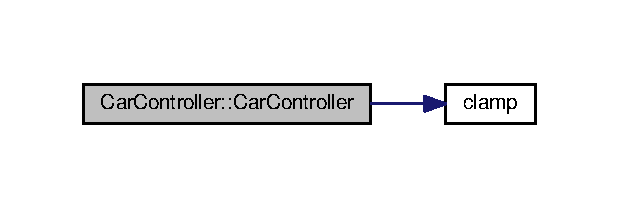
\includegraphics[width=297pt]{class_car_controller_a264969d4b9580b41b7e6d573a18b1de0_cgraph}
\end{center}
\end{figure}




The documentation for this class was generated from the following files\+:\begin{DoxyCompactItemize}
\item 
/home/travis/build/\+Autonomous-\/\+Racing-\/\+P\+G/ros.\+package/docs/master/ros\+\_\+ws/src/car\+\_\+control/include/\hyperlink{car__controller_8h}{car\+\_\+controller.\+h}\item 
/home/travis/build/\+Autonomous-\/\+Racing-\/\+P\+G/ros.\+package/docs/master/ros\+\_\+ws/src/car\+\_\+control/src/\hyperlink{car__controller_8cpp}{car\+\_\+controller.\+cpp}\end{DoxyCompactItemize}

\hypertarget{classcircle_1_1_circle}{}\section{circle.\+Circle Class Reference}
\label{classcircle_1_1_circle}\index{circle.\+Circle@{circle.\+Circle}}
\subsection*{Public Member Functions}
\begin{DoxyCompactItemize}
\item 
def \hyperlink{classcircle_1_1_circle_ae5573aa3ec1e6df913e13c01cf3ed7b9}{\+\_\+\+\_\+init\+\_\+\+\_\+} (self, \hyperlink{classcircle_1_1_circle_aa2ed466736c7e4436ab6ded456ebd24b}{center}, \hyperlink{classcircle_1_1_circle_a33aec6cd768f0a1850fae92cf3fcbc95}{radius})
\item 
def \hyperlink{classcircle_1_1_circle_a95ddced3abdbd659ea243a1d420a8c6c}{create\+\_\+array} (self, start\+\_\+angle, end\+\_\+angle, sample\+\_\+count=50)
\item 
def \hyperlink{classcircle_1_1_circle_a1ec1a241492841bc729e660788684407}{get\+\_\+angle} (self, point)
\item 
def \hyperlink{classcircle_1_1_circle_a191eb7323e7138ce625cc345822bff17}{get\+\_\+closest\+\_\+point} (self, point)
\end{DoxyCompactItemize}
\subsection*{Static Public Member Functions}
\begin{DoxyCompactItemize}
\item 
def \hyperlink{classcircle_1_1_circle_a755e5bf15cddcd1a3e20804ece765aba}{fit} (points)
\end{DoxyCompactItemize}
\subsection*{Public Attributes}
\begin{DoxyCompactItemize}
\item 
\hyperlink{classcircle_1_1_circle_aa2ed466736c7e4436ab6ded456ebd24b}{center}
\item 
\hyperlink{classcircle_1_1_circle_a33aec6cd768f0a1850fae92cf3fcbc95}{radius}
\end{DoxyCompactItemize}


\subsection{Detailed Description}


Definition at line 11 of file circle.\+py.



\subsection{Constructor \& Destructor Documentation}
\index{circle\+::\+Circle@{circle\+::\+Circle}!\+\_\+\+\_\+init\+\_\+\+\_\+@{\+\_\+\+\_\+init\+\_\+\+\_\+}}
\index{\+\_\+\+\_\+init\+\_\+\+\_\+@{\+\_\+\+\_\+init\+\_\+\+\_\+}!circle\+::\+Circle@{circle\+::\+Circle}}
\subsubsection[{\texorpdfstring{\+\_\+\+\_\+init\+\_\+\+\_\+(self, center, radius)}{__init__(self, center, radius)}}]{\setlength{\rightskip}{0pt plus 5cm}def circle.\+Circle.\+\_\+\+\_\+init\+\_\+\+\_\+ (
\begin{DoxyParamCaption}
\item[{}]{self, }
\item[{}]{center, }
\item[{}]{radius}
\end{DoxyParamCaption}
)}\hypertarget{classcircle_1_1_circle_ae5573aa3ec1e6df913e13c01cf3ed7b9}{}\label{classcircle_1_1_circle_ae5573aa3ec1e6df913e13c01cf3ed7b9}


Definition at line 12 of file circle.\+py.



\subsection{Member Function Documentation}
\index{circle\+::\+Circle@{circle\+::\+Circle}!create\+\_\+array@{create\+\_\+array}}
\index{create\+\_\+array@{create\+\_\+array}!circle\+::\+Circle@{circle\+::\+Circle}}
\subsubsection[{\texorpdfstring{create\+\_\+array(self, start\+\_\+angle, end\+\_\+angle, sample\+\_\+count=50)}{create_array(self, start_angle, end_angle, sample_count=50)}}]{\setlength{\rightskip}{0pt plus 5cm}def circle.\+Circle.\+create\+\_\+array (
\begin{DoxyParamCaption}
\item[{}]{self, }
\item[{}]{start\+\_\+angle, }
\item[{}]{end\+\_\+angle, }
\item[{}]{sample\+\_\+count = {\ttfamily 50}}
\end{DoxyParamCaption}
)}\hypertarget{classcircle_1_1_circle_a95ddced3abdbd659ea243a1d420a8c6c}{}\label{classcircle_1_1_circle_a95ddced3abdbd659ea243a1d420a8c6c}


Definition at line 16 of file circle.\+py.

\index{circle\+::\+Circle@{circle\+::\+Circle}!fit@{fit}}
\index{fit@{fit}!circle\+::\+Circle@{circle\+::\+Circle}}
\subsubsection[{\texorpdfstring{fit(points)}{fit(points)}}]{\setlength{\rightskip}{0pt plus 5cm}def circle.\+Circle.\+fit (
\begin{DoxyParamCaption}
\item[{}]{points}
\end{DoxyParamCaption}
)\hspace{0.3cm}{\ttfamily [static]}}\hypertarget{classcircle_1_1_circle_a755e5bf15cddcd1a3e20804ece765aba}{}\label{classcircle_1_1_circle_a755e5bf15cddcd1a3e20804ece765aba}


Definition at line 36 of file circle.\+py.

\index{circle\+::\+Circle@{circle\+::\+Circle}!get\+\_\+angle@{get\+\_\+angle}}
\index{get\+\_\+angle@{get\+\_\+angle}!circle\+::\+Circle@{circle\+::\+Circle}}
\subsubsection[{\texorpdfstring{get\+\_\+angle(self, point)}{get_angle(self, point)}}]{\setlength{\rightskip}{0pt plus 5cm}def circle.\+Circle.\+get\+\_\+angle (
\begin{DoxyParamCaption}
\item[{}]{self, }
\item[{}]{point}
\end{DoxyParamCaption}
)}\hypertarget{classcircle_1_1_circle_a1ec1a241492841bc729e660788684407}{}\label{classcircle_1_1_circle_a1ec1a241492841bc729e660788684407}


Definition at line 23 of file circle.\+py.

\index{circle\+::\+Circle@{circle\+::\+Circle}!get\+\_\+closest\+\_\+point@{get\+\_\+closest\+\_\+point}}
\index{get\+\_\+closest\+\_\+point@{get\+\_\+closest\+\_\+point}!circle\+::\+Circle@{circle\+::\+Circle}}
\subsubsection[{\texorpdfstring{get\+\_\+closest\+\_\+point(self, point)}{get_closest_point(self, point)}}]{\setlength{\rightskip}{0pt plus 5cm}def circle.\+Circle.\+get\+\_\+closest\+\_\+point (
\begin{DoxyParamCaption}
\item[{}]{self, }
\item[{}]{point}
\end{DoxyParamCaption}
)}\hypertarget{classcircle_1_1_circle_a191eb7323e7138ce625cc345822bff17}{}\label{classcircle_1_1_circle_a191eb7323e7138ce625cc345822bff17}


Definition at line 26 of file circle.\+py.



\subsection{Member Data Documentation}
\index{circle\+::\+Circle@{circle\+::\+Circle}!center@{center}}
\index{center@{center}!circle\+::\+Circle@{circle\+::\+Circle}}
\subsubsection[{\texorpdfstring{center}{center}}]{\setlength{\rightskip}{0pt plus 5cm}circle.\+Circle.\+center}\hypertarget{classcircle_1_1_circle_aa2ed466736c7e4436ab6ded456ebd24b}{}\label{classcircle_1_1_circle_aa2ed466736c7e4436ab6ded456ebd24b}


Definition at line 13 of file circle.\+py.

\index{circle\+::\+Circle@{circle\+::\+Circle}!radius@{radius}}
\index{radius@{radius}!circle\+::\+Circle@{circle\+::\+Circle}}
\subsubsection[{\texorpdfstring{radius}{radius}}]{\setlength{\rightskip}{0pt plus 5cm}circle.\+Circle.\+radius}\hypertarget{classcircle_1_1_circle_a33aec6cd768f0a1850fae92cf3fcbc95}{}\label{classcircle_1_1_circle_a33aec6cd768f0a1850fae92cf3fcbc95}


Definition at line 14 of file circle.\+py.



The documentation for this class was generated from the following file\+:\begin{DoxyCompactItemize}
\item 
/home/travis/build/\+Autonomous-\/\+Racing-\/\+P\+G/ar-\/tu-\/do/docs/master/ros\+\_\+ws/src/autonomous/wallfollowing2/script/\hyperlink{circle_8py}{circle.\+py}\end{DoxyCompactItemize}

\hypertarget{class_crash_detector}{}\section{Crash\+Detector Class Reference}
\label{class_crash_detector}\index{Crash\+Detector@{Crash\+Detector}}


R\+OS node that listens on a gazebo topic for collisions and publishes to a R\+OS topic.  




{\ttfamily \#include $<$crash\+\_\+detector.\+h$>$}

\subsection*{Public Member Functions}
\begin{DoxyCompactItemize}
\item 
\hyperlink{class_crash_detector_a4ee1c57168019f26a8f3b3263350a306}{Crash\+Detector} ()
\end{DoxyCompactItemize}


\subsection{Detailed Description}
R\+OS node that listens on a gazebo topic for collisions and publishes to a R\+OS topic. 

Definition at line 19 of file crash\+\_\+detector.\+h.



\subsection{Constructor \& Destructor Documentation}
\index{Crash\+Detector@{Crash\+Detector}!Crash\+Detector@{Crash\+Detector}}
\index{Crash\+Detector@{Crash\+Detector}!Crash\+Detector@{Crash\+Detector}}
\subsubsection[{\texorpdfstring{Crash\+Detector()}{CrashDetector()}}]{\setlength{\rightskip}{0pt plus 5cm}Crash\+Detector\+::\+Crash\+Detector (
\begin{DoxyParamCaption}
{}
\end{DoxyParamCaption}
)}\hypertarget{class_crash_detector_a4ee1c57168019f26a8f3b3263350a306}{}\label{class_crash_detector_a4ee1c57168019f26a8f3b3263350a306}


Definition at line 3 of file crash\+\_\+detector.\+cpp.



The documentation for this class was generated from the following files\+:\begin{DoxyCompactItemize}
\item 
/home/travis/build/\+Autonomous-\/\+Racing-\/\+P\+G/ros.\+package/docs/master/ros\+\_\+ws/src/simulation/simulation\+\_\+tools/include/\hyperlink{crash__detector_8h}{crash\+\_\+detector.\+h}\item 
/home/travis/build/\+Autonomous-\/\+Racing-\/\+P\+G/ros.\+package/docs/master/ros\+\_\+ws/src/simulation/simulation\+\_\+tools/src/\hyperlink{crash__detector_8cpp}{crash\+\_\+detector.\+cpp}\end{DoxyCompactItemize}

\hypertarget{class_d_m_s_controller}{}\section{D\+M\+S\+Controller Class Reference}
\label{class_d_m_s_controller}\index{D\+M\+S\+Controller@{D\+M\+S\+Controller}}


{\ttfamily \#include $<$dms\+\_\+controller.\+h$>$}

\subsection*{Public Member Functions}
\begin{DoxyCompactItemize}
\item 
\hyperlink{class_d_m_s_controller_acf8a9f7eb6ca02674679d5205253a0f9}{D\+M\+S\+Controller} ()
\item 
void \hyperlink{class_d_m_s_controller_a4260d418f52da772f8b7704607df86b0}{spin} ()
\end{DoxyCompactItemize}


\subsection{Detailed Description}


Definition at line 23 of file dms\+\_\+controller.\+h.



\subsection{Constructor \& Destructor Documentation}
\index{D\+M\+S\+Controller@{D\+M\+S\+Controller}!D\+M\+S\+Controller@{D\+M\+S\+Controller}}
\index{D\+M\+S\+Controller@{D\+M\+S\+Controller}!D\+M\+S\+Controller@{D\+M\+S\+Controller}}
\subsubsection[{\texorpdfstring{D\+M\+S\+Controller()}{DMSController()}}]{\setlength{\rightskip}{0pt plus 5cm}D\+M\+S\+Controller\+::\+D\+M\+S\+Controller (
\begin{DoxyParamCaption}
{}
\end{DoxyParamCaption}
)}\hypertarget{class_d_m_s_controller_acf8a9f7eb6ca02674679d5205253a0f9}{}\label{class_d_m_s_controller_acf8a9f7eb6ca02674679d5205253a0f9}


Definition at line 3 of file dms\+\_\+controller.\+cpp.



\subsection{Member Function Documentation}
\index{D\+M\+S\+Controller@{D\+M\+S\+Controller}!spin@{spin}}
\index{spin@{spin}!D\+M\+S\+Controller@{D\+M\+S\+Controller}}
\subsubsection[{\texorpdfstring{spin()}{spin()}}]{\setlength{\rightskip}{0pt plus 5cm}void D\+M\+S\+Controller\+::spin (
\begin{DoxyParamCaption}
{}
\end{DoxyParamCaption}
)}\hypertarget{class_d_m_s_controller_a4260d418f52da772f8b7704607df86b0}{}\label{class_d_m_s_controller_a4260d418f52da772f8b7704607df86b0}


Definition at line 23 of file dms\+\_\+controller.\+cpp.



Here is the caller graph for this function\+:
\nopagebreak
\begin{figure}[H]
\begin{center}
\leavevmode
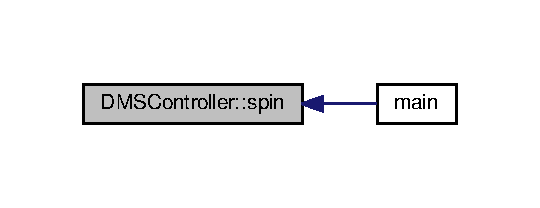
\includegraphics[width=259pt]{class_d_m_s_controller_a4260d418f52da772f8b7704607df86b0_icgraph}
\end{center}
\end{figure}




The documentation for this class was generated from the following files\+:\begin{DoxyCompactItemize}
\item 
/home/travis/build/\+Autonomous-\/\+Racing-\/\+P\+G/ar-\/tu-\/do/docs/master/ros\+\_\+ws/src/car\+\_\+control/include/\hyperlink{dms__controller_8h}{dms\+\_\+controller.\+h}\item 
/home/travis/build/\+Autonomous-\/\+Racing-\/\+P\+G/ar-\/tu-\/do/docs/master/ros\+\_\+ws/src/car\+\_\+control/src/\hyperlink{dms__controller_8cpp}{dms\+\_\+controller.\+cpp}\end{DoxyCompactItemize}

\hypertarget{class_drive_parameters_multiplexer}{}\section{Drive\+Parameters\+Multiplexer Class Reference}
\label{class_drive_parameters_multiplexer}\index{Drive\+Parameters\+Multiplexer@{Drive\+Parameters\+Multiplexer}}


{\ttfamily \#include $<$drive\+\_\+parameters\+\_\+multiplexer.\+h$>$}

\subsection*{Public Member Functions}
\begin{DoxyCompactItemize}
\item 
\hyperlink{class_drive_parameters_multiplexer_a00fd5b0e6d1d76fce05212c78310bebc}{Drive\+Parameters\+Multiplexer} ()
\begin{DoxyCompactList}\small\item\em Construct a new \hyperlink{class_drive_parameters_multiplexer}{Drive\+Parameters\+Multiplexer} object and initialize sources for all publishers of drive parameters. \end{DoxyCompactList}\end{DoxyCompactItemize}


\subsection{Detailed Description}


Definition at line 21 of file drive\+\_\+parameters\+\_\+multiplexer.\+h.



\subsection{Constructor \& Destructor Documentation}
\index{Drive\+Parameters\+Multiplexer@{Drive\+Parameters\+Multiplexer}!Drive\+Parameters\+Multiplexer@{Drive\+Parameters\+Multiplexer}}
\index{Drive\+Parameters\+Multiplexer@{Drive\+Parameters\+Multiplexer}!Drive\+Parameters\+Multiplexer@{Drive\+Parameters\+Multiplexer}}
\subsubsection[{\texorpdfstring{Drive\+Parameters\+Multiplexer()}{DriveParametersMultiplexer()}}]{\setlength{\rightskip}{0pt plus 5cm}Drive\+Parameters\+Multiplexer\+::\+Drive\+Parameters\+Multiplexer (
\begin{DoxyParamCaption}
{}
\end{DoxyParamCaption}
)}\hypertarget{class_drive_parameters_multiplexer_a00fd5b0e6d1d76fce05212c78310bebc}{}\label{class_drive_parameters_multiplexer_a00fd5b0e6d1d76fce05212c78310bebc}


Construct a new \hyperlink{class_drive_parameters_multiplexer}{Drive\+Parameters\+Multiplexer} object and initialize sources for all publishers of drive parameters. 



Definition at line 3 of file drive\+\_\+parameters\+\_\+multiplexer.\+cpp.



Here is the call graph for this function\+:
\nopagebreak
\begin{figure}[H]
\begin{center}
\leavevmode
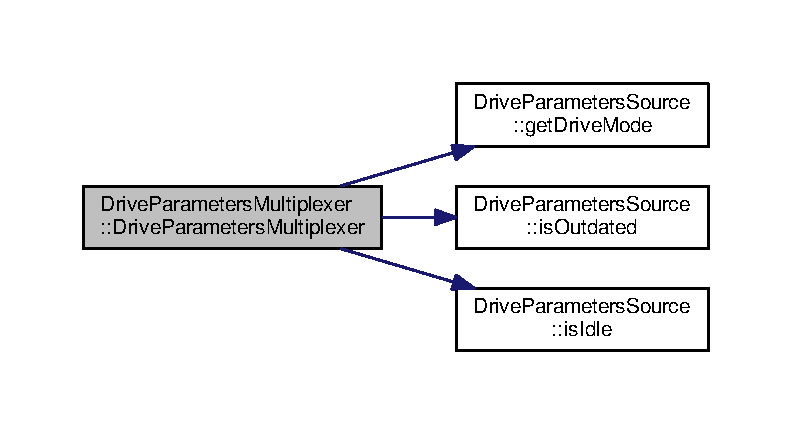
\includegraphics[width=350pt]{class_drive_parameters_multiplexer_a00fd5b0e6d1d76fce05212c78310bebc_cgraph}
\end{center}
\end{figure}




The documentation for this class was generated from the following files\+:\begin{DoxyCompactItemize}
\item 
/home/travis/build/\+Autonomous-\/\+Racing-\/\+P\+G/ar-\/tu-\/do/docs/master/ros\+\_\+ws/src/car\+\_\+control/include/\hyperlink{drive__parameters__multiplexer_8h}{drive\+\_\+parameters\+\_\+multiplexer.\+h}\item 
/home/travis/build/\+Autonomous-\/\+Racing-\/\+P\+G/ar-\/tu-\/do/docs/master/ros\+\_\+ws/src/car\+\_\+control/src/\hyperlink{drive__parameters__multiplexer_8cpp}{drive\+\_\+parameters\+\_\+multiplexer.\+cpp}\end{DoxyCompactItemize}

\hypertarget{class_drive_parameters_source}{}\section{Drive\+Parameters\+Source Class Reference}
\label{class_drive_parameters_source}\index{Drive\+Parameters\+Source@{Drive\+Parameters\+Source}}


{\ttfamily \#include $<$drive\+\_\+parameters\+\_\+source.\+h$>$}

\subsection*{Public Member Functions}
\begin{DoxyCompactItemize}
\item 
\hyperlink{class_drive_parameters_source_ab6ab4aa02955d8929ee04669faef1be2}{Drive\+Parameters\+Source} (ros\+::\+Node\+Handle $\ast$node\+\_\+handle, const char $\ast$topic, \hyperlink{drive__parameters__source_8h_a87328cd02ddd6c83ff6d4943cf8a93c2}{Drive\+Parameter\+Callback\+Function} update\+\_\+callback, int priority, double timeout)
\begin{DoxyCompactList}\small\item\em Construct a new \hyperlink{class_drive_parameters_source}{Drive\+Parameters\+Source} object, subscribes to the topic and stores the parameters into local variables. \end{DoxyCompactList}\item 
bool \hyperlink{class_drive_parameters_source_a19ac7507bffaa6167393d24fe5f7f67e}{is\+Outdated} ()
\begin{DoxyCompactList}\small\item\em Returns true if no update was received for a certain time, determined by the timeout variable. \end{DoxyCompactList}\item 
bool \hyperlink{class_drive_parameters_source_a716e9da760080cdc8d0e69553932c789}{is\+Idle} ()
\begin{DoxyCompactList}\small\item\em Returns true if the last update contained values close to 0 for both steering and throttle. If no update was received yet, this returns true. \end{DoxyCompactList}\item 
int \hyperlink{class_drive_parameters_source_a0ca68bb4cf93f5124c60330582ba82dc}{get\+Priority} ()
\begin{DoxyCompactList}\small\item\em Returns the priority of the source. If multiple sources are not idle, the source with the highest priority is forwarded. \end{DoxyCompactList}\end{DoxyCompactItemize}


\subsection{Detailed Description}


Definition at line 19 of file drive\+\_\+parameters\+\_\+source.\+h.



\subsection{Constructor \& Destructor Documentation}
\index{Drive\+Parameters\+Source@{Drive\+Parameters\+Source}!Drive\+Parameters\+Source@{Drive\+Parameters\+Source}}
\index{Drive\+Parameters\+Source@{Drive\+Parameters\+Source}!Drive\+Parameters\+Source@{Drive\+Parameters\+Source}}
\subsubsection[{\texorpdfstring{Drive\+Parameters\+Source(ros\+::\+Node\+Handle $\ast$node\+\_\+handle, const char $\ast$topic, Drive\+Parameter\+Callback\+Function update\+\_\+callback, int priority, double timeout)}{DriveParametersSource(ros::NodeHandle *node_handle, const char *topic, DriveParameterCallbackFunction update_callback, int priority, double timeout)}}]{\setlength{\rightskip}{0pt plus 5cm}Drive\+Parameters\+Source\+::\+Drive\+Parameters\+Source (
\begin{DoxyParamCaption}
\item[{ros\+::\+Node\+Handle $\ast$}]{node\+\_\+handle, }
\item[{const char $\ast$}]{topic, }
\item[{{\bf Drive\+Parameter\+Callback\+Function}}]{update\+\_\+callback, }
\item[{int}]{priority, }
\item[{double}]{timeout}
\end{DoxyParamCaption}
)}\hypertarget{class_drive_parameters_source_ab6ab4aa02955d8929ee04669faef1be2}{}\label{class_drive_parameters_source_ab6ab4aa02955d8929ee04669faef1be2}


Construct a new \hyperlink{class_drive_parameters_source}{Drive\+Parameters\+Source} object, subscribes to the topic and stores the parameters into local variables. 


\begin{DoxyParams}{Parameters}
{\em node\+\_\+handle} & A node handle is needed to create a topic subscriber \\
\hline
{\em topic} & The name of the drive\+\_\+param topic to subscribe to \\
\hline
{\em update\+\_\+callback} & Callback function that will be called whenever a message was received \\
\hline
{\em priority} & Priority of the source. If multiple sources are not idle, the source with the highest priority is forwarded. \\
\hline
{\em timeout} & Messages will be deferred when they are older than this, in seconds. \\
\hline
\end{DoxyParams}


Definition at line 6 of file drive\+\_\+parameters\+\_\+source.\+cpp.



\subsection{Member Function Documentation}
\index{Drive\+Parameters\+Source@{Drive\+Parameters\+Source}!get\+Priority@{get\+Priority}}
\index{get\+Priority@{get\+Priority}!Drive\+Parameters\+Source@{Drive\+Parameters\+Source}}
\subsubsection[{\texorpdfstring{get\+Priority()}{getPriority()}}]{\setlength{\rightskip}{0pt plus 5cm}int Drive\+Parameters\+Source\+::get\+Priority (
\begin{DoxyParamCaption}
{}
\end{DoxyParamCaption}
)}\hypertarget{class_drive_parameters_source_a0ca68bb4cf93f5124c60330582ba82dc}{}\label{class_drive_parameters_source_a0ca68bb4cf93f5124c60330582ba82dc}


Returns the priority of the source. If multiple sources are not idle, the source with the highest priority is forwarded. 



Definition at line 41 of file drive\+\_\+parameters\+\_\+source.\+cpp.



Here is the caller graph for this function\+:
\nopagebreak
\begin{figure}[H]
\begin{center}
\leavevmode
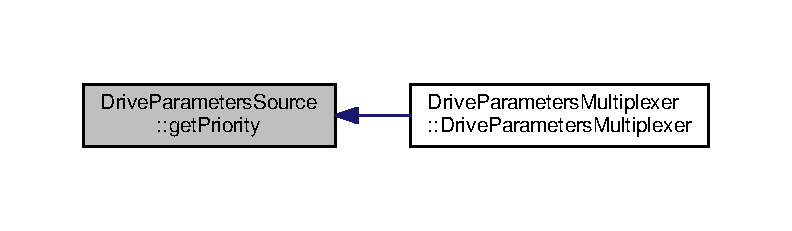
\includegraphics[width=350pt]{class_drive_parameters_source_a0ca68bb4cf93f5124c60330582ba82dc_icgraph}
\end{center}
\end{figure}


\index{Drive\+Parameters\+Source@{Drive\+Parameters\+Source}!is\+Idle@{is\+Idle}}
\index{is\+Idle@{is\+Idle}!Drive\+Parameters\+Source@{Drive\+Parameters\+Source}}
\subsubsection[{\texorpdfstring{is\+Idle()}{isIdle()}}]{\setlength{\rightskip}{0pt plus 5cm}bool Drive\+Parameters\+Source\+::is\+Idle (
\begin{DoxyParamCaption}
{}
\end{DoxyParamCaption}
)}\hypertarget{class_drive_parameters_source_a716e9da760080cdc8d0e69553932c789}{}\label{class_drive_parameters_source_a716e9da760080cdc8d0e69553932c789}


Returns true if the last update contained values close to 0 for both steering and throttle. If no update was received yet, this returns true. 



Definition at line 36 of file drive\+\_\+parameters\+\_\+source.\+cpp.



Here is the caller graph for this function\+:
\nopagebreak
\begin{figure}[H]
\begin{center}
\leavevmode
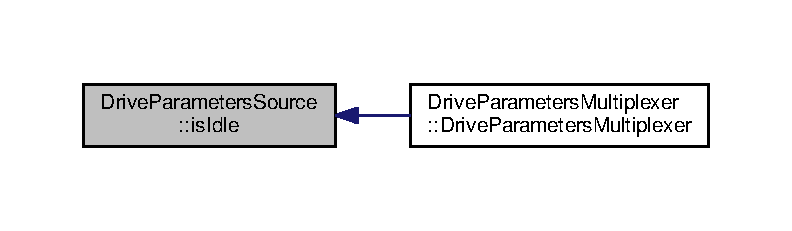
\includegraphics[width=350pt]{class_drive_parameters_source_a716e9da760080cdc8d0e69553932c789_icgraph}
\end{center}
\end{figure}


\index{Drive\+Parameters\+Source@{Drive\+Parameters\+Source}!is\+Outdated@{is\+Outdated}}
\index{is\+Outdated@{is\+Outdated}!Drive\+Parameters\+Source@{Drive\+Parameters\+Source}}
\subsubsection[{\texorpdfstring{is\+Outdated()}{isOutdated()}}]{\setlength{\rightskip}{0pt plus 5cm}bool Drive\+Parameters\+Source\+::is\+Outdated (
\begin{DoxyParamCaption}
{}
\end{DoxyParamCaption}
)}\hypertarget{class_drive_parameters_source_a19ac7507bffaa6167393d24fe5f7f67e}{}\label{class_drive_parameters_source_a19ac7507bffaa6167393d24fe5f7f67e}


Returns true if no update was received for a certain time, determined by the timeout variable. 



Definition at line 27 of file drive\+\_\+parameters\+\_\+source.\+cpp.



Here is the caller graph for this function\+:
\nopagebreak
\begin{figure}[H]
\begin{center}
\leavevmode
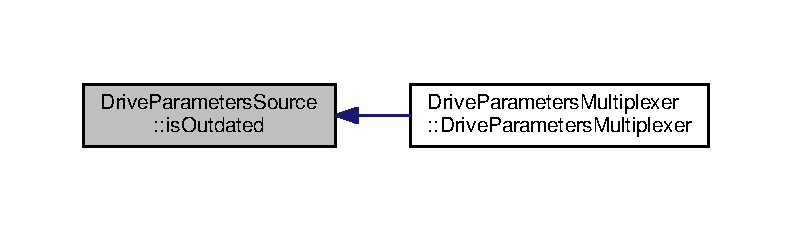
\includegraphics[width=350pt]{class_drive_parameters_source_a19ac7507bffaa6167393d24fe5f7f67e_icgraph}
\end{center}
\end{figure}




The documentation for this class was generated from the following files\+:\begin{DoxyCompactItemize}
\item 
/home/travis/build/\+Autonomous-\/\+Racing-\/\+P\+G/ros.\+package/docs/master/ros\+\_\+ws/src/car\+\_\+control/include/\hyperlink{drive__parameters__source_8h}{drive\+\_\+parameters\+\_\+source.\+h}\item 
/home/travis/build/\+Autonomous-\/\+Racing-\/\+P\+G/ros.\+package/docs/master/ros\+\_\+ws/src/car\+\_\+control/src/\hyperlink{drive__parameters__source_8cpp}{drive\+\_\+parameters\+\_\+source.\+cpp}\end{DoxyCompactItemize}

\hypertarget{class_emergency_stop}{}\section{Emergency\+Stop Class Reference}
\label{class_emergency_stop}\index{Emergency\+Stop@{Emergency\+Stop}}


{\ttfamily \#include $<$emergency\+\_\+stop.\+h$>$}

\subsection*{Public Member Functions}
\begin{DoxyCompactItemize}
\item 
\hyperlink{class_emergency_stop_acd5c3e0c838fe697ebf95452199cca77}{Emergency\+Stop} ()
\end{DoxyCompactItemize}


\subsection{Detailed Description}


Definition at line 18 of file emergency\+\_\+stop.\+h.



\subsection{Constructor \& Destructor Documentation}
\index{Emergency\+Stop@{Emergency\+Stop}!Emergency\+Stop@{Emergency\+Stop}}
\index{Emergency\+Stop@{Emergency\+Stop}!Emergency\+Stop@{Emergency\+Stop}}
\subsubsection[{\texorpdfstring{Emergency\+Stop()}{EmergencyStop()}}]{\setlength{\rightskip}{0pt plus 5cm}Emergency\+Stop\+::\+Emergency\+Stop (
\begin{DoxyParamCaption}
{}
\end{DoxyParamCaption}
)}\hypertarget{class_emergency_stop_acd5c3e0c838fe697ebf95452199cca77}{}\label{class_emergency_stop_acd5c3e0c838fe697ebf95452199cca77}


Definition at line 3 of file emergency\+\_\+stop.\+cpp.



The documentation for this class was generated from the following files\+:\begin{DoxyCompactItemize}
\item 
/home/travis/build/\+Autonomous-\/\+Racing-\/\+P\+G/ros.\+package/docs/master/ros\+\_\+ws/src/autonomous/include/\hyperlink{emergency__stop_8h}{emergency\+\_\+stop.\+h}\item 
/home/travis/build/\+Autonomous-\/\+Racing-\/\+P\+G/ros.\+package/docs/master/ros\+\_\+ws/src/autonomous/src/\hyperlink{emergency__stop_8cpp}{emergency\+\_\+stop.\+cpp}\end{DoxyCompactItemize}

\hypertarget{class_joystick_controller}{}\section{Joystick\+Controller Class Reference}
\label{class_joystick_controller}\index{Joystick\+Controller@{Joystick\+Controller}}


{\ttfamily \#include $<$joystick\+\_\+controller.\+h$>$}

\subsection*{Public Member Functions}
\begin{DoxyCompactItemize}
\item 
\hyperlink{class_joystick_controller_aa7ba7d1b336933c7431ac8796b43c898}{Joystick\+Controller} ()
\begin{DoxyCompactList}\small\item\em Construct a new Remote Joy\+:\+: Remote Joy object. \end{DoxyCompactList}\end{DoxyCompactItemize}


\subsection{Detailed Description}


Definition at line 18 of file joystick\+\_\+controller.\+h.



\subsection{Constructor \& Destructor Documentation}
\index{Joystick\+Controller@{Joystick\+Controller}!Joystick\+Controller@{Joystick\+Controller}}
\index{Joystick\+Controller@{Joystick\+Controller}!Joystick\+Controller@{Joystick\+Controller}}
\subsubsection[{\texorpdfstring{Joystick\+Controller()}{JoystickController()}}]{\setlength{\rightskip}{0pt plus 5cm}Joystick\+Controller\+::\+Joystick\+Controller (
\begin{DoxyParamCaption}
{}
\end{DoxyParamCaption}
)}\hypertarget{class_joystick_controller_aa7ba7d1b336933c7431ac8796b43c898}{}\label{class_joystick_controller_aa7ba7d1b336933c7431ac8796b43c898}


Construct a new Remote Joy\+:\+: Remote Joy object. 



Definition at line 6 of file joystick\+\_\+controller.\+cpp.



The documentation for this class was generated from the following files\+:\begin{DoxyCompactItemize}
\item 
/home/travis/build/\+Autonomous-\/\+Racing-\/\+P\+G/ros.\+package/docs/master/ros\+\_\+ws/src/teleoperation/include/\hyperlink{joystick__controller_8h}{joystick\+\_\+controller.\+h}\item 
/home/travis/build/\+Autonomous-\/\+Racing-\/\+P\+G/ros.\+package/docs/master/ros\+\_\+ws/src/teleoperation/src/\hyperlink{joystick__controller_8cpp}{joystick\+\_\+controller.\+cpp}\end{DoxyCompactItemize}

\hypertarget{class_keyboard_controller}{}\section{Keyboard\+Controller Class Reference}
\label{class_keyboard_controller}\index{Keyboard\+Controller@{Keyboard\+Controller}}


{\ttfamily \#include $<$keyboard\+\_\+controller.\+h$>$}

\subsection*{Public Member Functions}
\begin{DoxyCompactItemize}
\item 
\hyperlink{class_keyboard_controller_abb80b5bae04a1c3cf904924cbacb235c}{Keyboard\+Controller} ()
\item 
\hyperlink{class_keyboard_controller_a102c3356ac118b886b6b5fb7a33245c1}{Keyboard\+Controller} (\hyperlink{class_keyboard_controller}{Keyboard\+Controller} \&\&)=default
\item 
\hyperlink{class_keyboard_controller_a0ea88596f23dbdfa81c80c8c72713957}{Keyboard\+Controller} (const \hyperlink{class_keyboard_controller}{Keyboard\+Controller} \&)=default
\item 
\hyperlink{class_keyboard_controller_a9791aa6d6fadf77b4ef3e59cdb7d9b1d}{$\sim$\+Keyboard\+Controller} ()
\end{DoxyCompactItemize}


\subsection{Detailed Description}


Definition at line 70 of file keyboard\+\_\+controller.\+h.



\subsection{Constructor \& Destructor Documentation}
\index{Keyboard\+Controller@{Keyboard\+Controller}!Keyboard\+Controller@{Keyboard\+Controller}}
\index{Keyboard\+Controller@{Keyboard\+Controller}!Keyboard\+Controller@{Keyboard\+Controller}}
\subsubsection[{\texorpdfstring{Keyboard\+Controller()}{KeyboardController()}}]{\setlength{\rightskip}{0pt plus 5cm}Keyboard\+Controller\+::\+Keyboard\+Controller (
\begin{DoxyParamCaption}
{}
\end{DoxyParamCaption}
)}\hypertarget{class_keyboard_controller_abb80b5bae04a1c3cf904924cbacb235c}{}\label{class_keyboard_controller_abb80b5bae04a1c3cf904924cbacb235c}
Class constructor that sets up a publisher for the drive parameters topic, creates a window and starts a timer for the main loop 

Definition at line 15 of file keyboard\+\_\+controller.\+cpp.

\index{Keyboard\+Controller@{Keyboard\+Controller}!Keyboard\+Controller@{Keyboard\+Controller}}
\index{Keyboard\+Controller@{Keyboard\+Controller}!Keyboard\+Controller@{Keyboard\+Controller}}
\subsubsection[{\texorpdfstring{Keyboard\+Controller(\+Keyboard\+Controller \&\&)=default}{KeyboardController(KeyboardController &&)=default}}]{\setlength{\rightskip}{0pt plus 5cm}Keyboard\+Controller\+::\+Keyboard\+Controller (
\begin{DoxyParamCaption}
\item[{{\bf Keyboard\+Controller} \&\&}]{}
\end{DoxyParamCaption}
)\hspace{0.3cm}{\ttfamily [default]}}\hypertarget{class_keyboard_controller_a102c3356ac118b886b6b5fb7a33245c1}{}\label{class_keyboard_controller_a102c3356ac118b886b6b5fb7a33245c1}
\index{Keyboard\+Controller@{Keyboard\+Controller}!Keyboard\+Controller@{Keyboard\+Controller}}
\index{Keyboard\+Controller@{Keyboard\+Controller}!Keyboard\+Controller@{Keyboard\+Controller}}
\subsubsection[{\texorpdfstring{Keyboard\+Controller(const Keyboard\+Controller \&)=default}{KeyboardController(const KeyboardController &)=default}}]{\setlength{\rightskip}{0pt plus 5cm}Keyboard\+Controller\+::\+Keyboard\+Controller (
\begin{DoxyParamCaption}
\item[{const {\bf Keyboard\+Controller} \&}]{}
\end{DoxyParamCaption}
)\hspace{0.3cm}{\ttfamily [default]}}\hypertarget{class_keyboard_controller_a0ea88596f23dbdfa81c80c8c72713957}{}\label{class_keyboard_controller_a0ea88596f23dbdfa81c80c8c72713957}
\index{Keyboard\+Controller@{Keyboard\+Controller}!````~Keyboard\+Controller@{$\sim$\+Keyboard\+Controller}}
\index{````~Keyboard\+Controller@{$\sim$\+Keyboard\+Controller}!Keyboard\+Controller@{Keyboard\+Controller}}
\subsubsection[{\texorpdfstring{$\sim$\+Keyboard\+Controller()}{~KeyboardController()}}]{\setlength{\rightskip}{0pt plus 5cm}Keyboard\+Controller\+::$\sim$\+Keyboard\+Controller (
\begin{DoxyParamCaption}
{}
\end{DoxyParamCaption}
)}\hypertarget{class_keyboard_controller_a9791aa6d6fadf77b4ef3e59cdb7d9b1d}{}\label{class_keyboard_controller_a9791aa6d6fadf77b4ef3e59cdb7d9b1d}


Definition at line 36 of file keyboard\+\_\+controller.\+cpp.



The documentation for this class was generated from the following files\+:\begin{DoxyCompactItemize}
\item 
/home/travis/build/\+Autonomous-\/\+Racing-\/\+P\+G/ros.\+package/docs/master/ros\+\_\+ws/src/teleoperation/include/\hyperlink{keyboard__controller_8h}{keyboard\+\_\+controller.\+h}\item 
/home/travis/build/\+Autonomous-\/\+Racing-\/\+P\+G/ros.\+package/docs/master/ros\+\_\+ws/src/teleoperation/src/\hyperlink{keyboard__controller_8cpp}{keyboard\+\_\+controller.\+cpp}\end{DoxyCompactItemize}

\hypertarget{class_laserscan_transformer}{}\section{Laserscan\+Transformer Class Reference}
\label{class_laserscan_transformer}\index{Laserscan\+Transformer@{Laserscan\+Transformer}}


This converter class converts a 2D laser scan as defined by sensor\+\_\+msgs/\+Laser\+Scan into a point cloud as defined by sensor\+\_\+msgs/\+Point\+Cloud2.  




{\ttfamily \#include $<$laserscan\+\_\+transformer.\+h$>$}

\subsection*{Public Member Functions}
\begin{DoxyCompactItemize}
\item 
\hyperlink{class_laserscan_transformer_a3fe9989fc225e8eaeea106f58db09db0}{Laserscan\+Transformer} ()
\end{DoxyCompactItemize}


\subsection{Detailed Description}
This converter class converts a 2D laser scan as defined by sensor\+\_\+msgs/\+Laser\+Scan into a point cloud as defined by sensor\+\_\+msgs/\+Point\+Cloud2. 

The main purpose of this class is the transformation of the Laser\+Scan to the \char`\"{}base\+\_\+link\char`\"{} of the racer model. 

Definition at line 24 of file laserscan\+\_\+transformer.\+h.



\subsection{Constructor \& Destructor Documentation}
\index{Laserscan\+Transformer@{Laserscan\+Transformer}!Laserscan\+Transformer@{Laserscan\+Transformer}}
\index{Laserscan\+Transformer@{Laserscan\+Transformer}!Laserscan\+Transformer@{Laserscan\+Transformer}}
\subsubsection[{\texorpdfstring{Laserscan\+Transformer()}{LaserscanTransformer()}}]{\setlength{\rightskip}{0pt plus 5cm}Laserscan\+Transformer\+::\+Laserscan\+Transformer (
\begin{DoxyParamCaption}
{}
\end{DoxyParamCaption}
)}\hypertarget{class_laserscan_transformer_a3fe9989fc225e8eaeea106f58db09db0}{}\label{class_laserscan_transformer_a3fe9989fc225e8eaeea106f58db09db0}


Definition at line 6 of file laserscan\+\_\+transformer.\+cpp.



The documentation for this class was generated from the following files\+:\begin{DoxyCompactItemize}
\item 
/home/travis/build/\+Autonomous-\/\+Racing-\/\+P\+G/ros.\+package/docs/master/ros\+\_\+ws/src/car\+\_\+tf/include/\hyperlink{laserscan__transformer_8h}{laserscan\+\_\+transformer.\+h}\item 
/home/travis/build/\+Autonomous-\/\+Racing-\/\+P\+G/ros.\+package/docs/master/ros\+\_\+ws/src/car\+\_\+tf/src/\hyperlink{laserscan__transformer_8cpp}{laserscan\+\_\+transformer.\+cpp}\end{DoxyCompactItemize}

\hypertarget{class_navigation_stack_control_converter}{}\section{Navigation\+Stack\+Control\+Converter Class Reference}
\label{class_navigation_stack_control_converter}\index{Navigation\+Stack\+Control\+Converter@{Navigation\+Stack\+Control\+Converter}}


This converter class converts \char`\"{}cmd\+\_\+vel\char`\"{} messages to \char`\"{}drive\+\_\+param\char`\"{} messages. The linear and angular velocity has to be transformed to linear velocity and steering angle. T\+O\+DO\+: Differential drive?  




{\ttfamily \#include $<$navigation\+\_\+stack\+\_\+control\+\_\+converter.\+h$>$}

\subsection*{Public Member Functions}
\begin{DoxyCompactItemize}
\item 
\hyperlink{class_navigation_stack_control_converter_aaa467e7f68ffb78c9778cdeedc972fac}{Navigation\+Stack\+Control\+Converter} ()
\begin{DoxyCompactList}\small\item\em Initializes the publisher and subscriber. \end{DoxyCompactList}\end{DoxyCompactItemize}


\subsection{Detailed Description}
This converter class converts \char`\"{}cmd\+\_\+vel\char`\"{} messages to \char`\"{}drive\+\_\+param\char`\"{} messages. The linear and angular velocity has to be transformed to linear velocity and steering angle. T\+O\+DO\+: Differential drive? 

Definition at line 16 of file navigation\+\_\+stack\+\_\+control\+\_\+converter.\+h.



\subsection{Constructor \& Destructor Documentation}
\index{Navigation\+Stack\+Control\+Converter@{Navigation\+Stack\+Control\+Converter}!Navigation\+Stack\+Control\+Converter@{Navigation\+Stack\+Control\+Converter}}
\index{Navigation\+Stack\+Control\+Converter@{Navigation\+Stack\+Control\+Converter}!Navigation\+Stack\+Control\+Converter@{Navigation\+Stack\+Control\+Converter}}
\subsubsection[{\texorpdfstring{Navigation\+Stack\+Control\+Converter()}{NavigationStackControlConverter()}}]{\setlength{\rightskip}{0pt plus 5cm}Navigation\+Stack\+Control\+Converter\+::\+Navigation\+Stack\+Control\+Converter (
\begin{DoxyParamCaption}
{}
\end{DoxyParamCaption}
)}\hypertarget{class_navigation_stack_control_converter_aaa467e7f68ffb78c9778cdeedc972fac}{}\label{class_navigation_stack_control_converter_aaa467e7f68ffb78c9778cdeedc972fac}


Initializes the publisher and subscriber. 



Definition at line 13 of file navigation\+\_\+stack\+\_\+control\+\_\+converter.\+cpp.



The documentation for this class was generated from the following files\+:\begin{DoxyCompactItemize}
\item 
/home/travis/build/\+Autonomous-\/\+Racing-\/\+P\+G/ros.\+package/docs/master/ros\+\_\+ws/src/navigation\+\_\+stack/msgs\+\_\+converter/include/\hyperlink{navigation__stack__control__converter_8h}{navigation\+\_\+stack\+\_\+control\+\_\+converter.\+h}\item 
/home/travis/build/\+Autonomous-\/\+Racing-\/\+P\+G/ros.\+package/docs/master/ros\+\_\+ws/src/navigation\+\_\+stack/msgs\+\_\+converter/src/\hyperlink{navigation__stack__control__converter_8cpp}{navigation\+\_\+stack\+\_\+control\+\_\+converter.\+cpp}\end{DoxyCompactItemize}

\hypertarget{classparameters_1_1_neural_q_estimator}{}\section{parameters.\+Neural\+Q\+Estimator Class Reference}
\label{classparameters_1_1_neural_q_estimator}\index{parameters.\+Neural\+Q\+Estimator@{parameters.\+Neural\+Q\+Estimator}}


Inheritance diagram for parameters.\+Neural\+Q\+Estimator\+:
\nopagebreak
\begin{figure}[H]
\begin{center}
\leavevmode
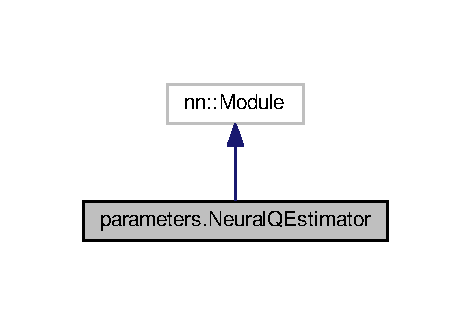
\includegraphics[width=226pt]{classparameters_1_1_neural_q_estimator__inherit__graph}
\end{center}
\end{figure}


Collaboration diagram for parameters.\+Neural\+Q\+Estimator\+:
\nopagebreak
\begin{figure}[H]
\begin{center}
\leavevmode
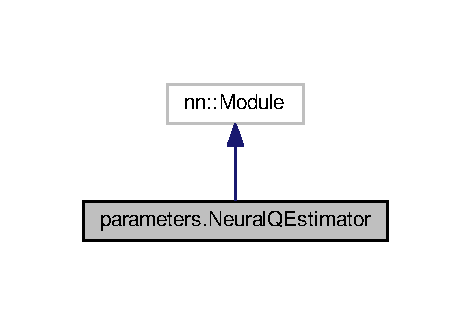
\includegraphics[width=226pt]{classparameters_1_1_neural_q_estimator__coll__graph}
\end{center}
\end{figure}
\subsection*{Public Member Functions}
\begin{DoxyCompactItemize}
\item 
def \hyperlink{classparameters_1_1_neural_q_estimator_ad820dedb1b53b0967f466939c69145c0}{\+\_\+\+\_\+init\+\_\+\+\_\+} (self)
\item 
def \hyperlink{classparameters_1_1_neural_q_estimator_acadb108832a386bbe20ad80015a2ed06}{forward} (self, x)
\item 
def \hyperlink{classparameters_1_1_neural_q_estimator_acd78f9e6bdd4cdda419ee5d83363ddd3}{load} (self)
\item 
def \hyperlink{classparameters_1_1_neural_q_estimator_a4efb1e7f7a7f77770cbd2a379ff2db8a}{save} (self)
\end{DoxyCompactItemize}
\subsection*{Public Attributes}
\begin{DoxyCompactItemize}
\item 
\hyperlink{classparameters_1_1_neural_q_estimator_ab0fb7d0e286565a2531f3ddb126e2592}{fc1}
\item 
\hyperlink{classparameters_1_1_neural_q_estimator_abd606711b39f423590adacb37c5b55d0}{fc2}
\item 
\hyperlink{classparameters_1_1_neural_q_estimator_ac48aa201a71a0e25e8ca7274a2cc5733}{fc3}
\end{DoxyCompactItemize}


\subsection{Detailed Description}


Definition at line 30 of file parameters.\+py.



\subsection{Constructor \& Destructor Documentation}
\index{parameters\+::\+Neural\+Q\+Estimator@{parameters\+::\+Neural\+Q\+Estimator}!\+\_\+\+\_\+init\+\_\+\+\_\+@{\+\_\+\+\_\+init\+\_\+\+\_\+}}
\index{\+\_\+\+\_\+init\+\_\+\+\_\+@{\+\_\+\+\_\+init\+\_\+\+\_\+}!parameters\+::\+Neural\+Q\+Estimator@{parameters\+::\+Neural\+Q\+Estimator}}
\subsubsection[{\texorpdfstring{\+\_\+\+\_\+init\+\_\+\+\_\+(self)}{__init__(self)}}]{\setlength{\rightskip}{0pt plus 5cm}def parameters.\+Neural\+Q\+Estimator.\+\_\+\+\_\+init\+\_\+\+\_\+ (
\begin{DoxyParamCaption}
\item[{}]{self}
\end{DoxyParamCaption}
)}\hypertarget{classparameters_1_1_neural_q_estimator_ad820dedb1b53b0967f466939c69145c0}{}\label{classparameters_1_1_neural_q_estimator_ad820dedb1b53b0967f466939c69145c0}


Definition at line 31 of file parameters.\+py.



\subsection{Member Function Documentation}
\index{parameters\+::\+Neural\+Q\+Estimator@{parameters\+::\+Neural\+Q\+Estimator}!forward@{forward}}
\index{forward@{forward}!parameters\+::\+Neural\+Q\+Estimator@{parameters\+::\+Neural\+Q\+Estimator}}
\subsubsection[{\texorpdfstring{forward(self, x)}{forward(self, x)}}]{\setlength{\rightskip}{0pt plus 5cm}def parameters.\+Neural\+Q\+Estimator.\+forward (
\begin{DoxyParamCaption}
\item[{}]{self, }
\item[{}]{x}
\end{DoxyParamCaption}
)}\hypertarget{classparameters_1_1_neural_q_estimator_acadb108832a386bbe20ad80015a2ed06}{}\label{classparameters_1_1_neural_q_estimator_acadb108832a386bbe20ad80015a2ed06}


Definition at line 37 of file parameters.\+py.

\index{parameters\+::\+Neural\+Q\+Estimator@{parameters\+::\+Neural\+Q\+Estimator}!load@{load}}
\index{load@{load}!parameters\+::\+Neural\+Q\+Estimator@{parameters\+::\+Neural\+Q\+Estimator}}
\subsubsection[{\texorpdfstring{load(self)}{load(self)}}]{\setlength{\rightskip}{0pt plus 5cm}def parameters.\+Neural\+Q\+Estimator.\+load (
\begin{DoxyParamCaption}
\item[{}]{self}
\end{DoxyParamCaption}
)}\hypertarget{classparameters_1_1_neural_q_estimator_acd78f9e6bdd4cdda419ee5d83363ddd3}{}\label{classparameters_1_1_neural_q_estimator_acd78f9e6bdd4cdda419ee5d83363ddd3}


Definition at line 42 of file parameters.\+py.

\index{parameters\+::\+Neural\+Q\+Estimator@{parameters\+::\+Neural\+Q\+Estimator}!save@{save}}
\index{save@{save}!parameters\+::\+Neural\+Q\+Estimator@{parameters\+::\+Neural\+Q\+Estimator}}
\subsubsection[{\texorpdfstring{save(self)}{save(self)}}]{\setlength{\rightskip}{0pt plus 5cm}def parameters.\+Neural\+Q\+Estimator.\+save (
\begin{DoxyParamCaption}
\item[{}]{self}
\end{DoxyParamCaption}
)}\hypertarget{classparameters_1_1_neural_q_estimator_a4efb1e7f7a7f77770cbd2a379ff2db8a}{}\label{classparameters_1_1_neural_q_estimator_a4efb1e7f7a7f77770cbd2a379ff2db8a}


Definition at line 47 of file parameters.\+py.



\subsection{Member Data Documentation}
\index{parameters\+::\+Neural\+Q\+Estimator@{parameters\+::\+Neural\+Q\+Estimator}!fc1@{fc1}}
\index{fc1@{fc1}!parameters\+::\+Neural\+Q\+Estimator@{parameters\+::\+Neural\+Q\+Estimator}}
\subsubsection[{\texorpdfstring{fc1}{fc1}}]{\setlength{\rightskip}{0pt plus 5cm}parameters.\+Neural\+Q\+Estimator.\+fc1}\hypertarget{classparameters_1_1_neural_q_estimator_ab0fb7d0e286565a2531f3ddb126e2592}{}\label{classparameters_1_1_neural_q_estimator_ab0fb7d0e286565a2531f3ddb126e2592}


Definition at line 33 of file parameters.\+py.

\index{parameters\+::\+Neural\+Q\+Estimator@{parameters\+::\+Neural\+Q\+Estimator}!fc2@{fc2}}
\index{fc2@{fc2}!parameters\+::\+Neural\+Q\+Estimator@{parameters\+::\+Neural\+Q\+Estimator}}
\subsubsection[{\texorpdfstring{fc2}{fc2}}]{\setlength{\rightskip}{0pt plus 5cm}parameters.\+Neural\+Q\+Estimator.\+fc2}\hypertarget{classparameters_1_1_neural_q_estimator_abd606711b39f423590adacb37c5b55d0}{}\label{classparameters_1_1_neural_q_estimator_abd606711b39f423590adacb37c5b55d0}


Definition at line 34 of file parameters.\+py.

\index{parameters\+::\+Neural\+Q\+Estimator@{parameters\+::\+Neural\+Q\+Estimator}!fc3@{fc3}}
\index{fc3@{fc3}!parameters\+::\+Neural\+Q\+Estimator@{parameters\+::\+Neural\+Q\+Estimator}}
\subsubsection[{\texorpdfstring{fc3}{fc3}}]{\setlength{\rightskip}{0pt plus 5cm}parameters.\+Neural\+Q\+Estimator.\+fc3}\hypertarget{classparameters_1_1_neural_q_estimator_ac48aa201a71a0e25e8ca7274a2cc5733}{}\label{classparameters_1_1_neural_q_estimator_ac48aa201a71a0e25e8ca7274a2cc5733}


Definition at line 35 of file parameters.\+py.



The documentation for this class was generated from the following file\+:\begin{DoxyCompactItemize}
\item 
/home/travis/build/\+Autonomous-\/\+Racing-\/\+P\+G/ros.\+package/docs/master/ros\+\_\+ws/src/autonomous/q\+\_\+learning/scripts/\hyperlink{parameters_8py}{parameters.\+py}\end{DoxyCompactItemize}

\hypertarget{classwallfollowing_1_1_parameters}{}\section{wallfollowing.\+Parameters Class Reference}
\label{classwallfollowing_1_1_parameters}\index{wallfollowing.\+Parameters@{wallfollowing.\+Parameters}}
\subsection*{Public Member Functions}
\begin{DoxyCompactItemize}
\item 
def \hyperlink{classwallfollowing_1_1_parameters_a471c55e861c60ca58f13a272ad4078d4}{\+\_\+\+\_\+init\+\_\+\+\_\+} (self, default\+\_\+values)
\item 
def \hyperlink{classwallfollowing_1_1_parameters_a7dfbcaac7a2060ce8c3623c8dfb2ed40}{load} (self)
\item 
def \hyperlink{classwallfollowing_1_1_parameters_a8391da200b442b6ee64c8befdc78ff48}{\+\_\+\+\_\+str\+\_\+\+\_\+} (self)
\end{DoxyCompactItemize}
\subsection*{Public Attributes}
\begin{DoxyCompactItemize}
\item 
\hyperlink{classwallfollowing_1_1_parameters_a009e7e6821f14f92f657fae2a7315313}{names}
\end{DoxyCompactItemize}


\subsection{Detailed Description}


Definition at line 53 of file wallfollowing.\+py.



\subsection{Constructor \& Destructor Documentation}
\index{wallfollowing\+::\+Parameters@{wallfollowing\+::\+Parameters}!\+\_\+\+\_\+init\+\_\+\+\_\+@{\+\_\+\+\_\+init\+\_\+\+\_\+}}
\index{\+\_\+\+\_\+init\+\_\+\+\_\+@{\+\_\+\+\_\+init\+\_\+\+\_\+}!wallfollowing\+::\+Parameters@{wallfollowing\+::\+Parameters}}
\subsubsection[{\texorpdfstring{\+\_\+\+\_\+init\+\_\+\+\_\+(self, default\+\_\+values)}{__init__(self, default_values)}}]{\setlength{\rightskip}{0pt plus 5cm}def wallfollowing.\+Parameters.\+\_\+\+\_\+init\+\_\+\+\_\+ (
\begin{DoxyParamCaption}
\item[{}]{self, }
\item[{}]{default\+\_\+values}
\end{DoxyParamCaption}
)}\hypertarget{classwallfollowing_1_1_parameters_a471c55e861c60ca58f13a272ad4078d4}{}\label{classwallfollowing_1_1_parameters_a471c55e861c60ca58f13a272ad4078d4}


Definition at line 54 of file wallfollowing.\+py.



\subsection{Member Function Documentation}
\index{wallfollowing\+::\+Parameters@{wallfollowing\+::\+Parameters}!\+\_\+\+\_\+str\+\_\+\+\_\+@{\+\_\+\+\_\+str\+\_\+\+\_\+}}
\index{\+\_\+\+\_\+str\+\_\+\+\_\+@{\+\_\+\+\_\+str\+\_\+\+\_\+}!wallfollowing\+::\+Parameters@{wallfollowing\+::\+Parameters}}
\subsubsection[{\texorpdfstring{\+\_\+\+\_\+str\+\_\+\+\_\+(self)}{__str__(self)}}]{\setlength{\rightskip}{0pt plus 5cm}def wallfollowing.\+Parameters.\+\_\+\+\_\+str\+\_\+\+\_\+ (
\begin{DoxyParamCaption}
\item[{}]{self}
\end{DoxyParamCaption}
)}\hypertarget{classwallfollowing_1_1_parameters_a8391da200b442b6ee64c8befdc78ff48}{}\label{classwallfollowing_1_1_parameters_a8391da200b442b6ee64c8befdc78ff48}


Definition at line 65 of file wallfollowing.\+py.

\index{wallfollowing\+::\+Parameters@{wallfollowing\+::\+Parameters}!load@{load}}
\index{load@{load}!wallfollowing\+::\+Parameters@{wallfollowing\+::\+Parameters}}
\subsubsection[{\texorpdfstring{load(self)}{load(self)}}]{\setlength{\rightskip}{0pt plus 5cm}def wallfollowing.\+Parameters.\+load (
\begin{DoxyParamCaption}
\item[{}]{self}
\end{DoxyParamCaption}
)}\hypertarget{classwallfollowing_1_1_parameters_a7dfbcaac7a2060ce8c3623c8dfb2ed40}{}\label{classwallfollowing_1_1_parameters_a7dfbcaac7a2060ce8c3623c8dfb2ed40}


Definition at line 59 of file wallfollowing.\+py.



\subsection{Member Data Documentation}
\index{wallfollowing\+::\+Parameters@{wallfollowing\+::\+Parameters}!names@{names}}
\index{names@{names}!wallfollowing\+::\+Parameters@{wallfollowing\+::\+Parameters}}
\subsubsection[{\texorpdfstring{names}{names}}]{\setlength{\rightskip}{0pt plus 5cm}wallfollowing.\+Parameters.\+names}\hypertarget{classwallfollowing_1_1_parameters_a009e7e6821f14f92f657fae2a7315313}{}\label{classwallfollowing_1_1_parameters_a009e7e6821f14f92f657fae2a7315313}


Definition at line 55 of file wallfollowing.\+py.



The documentation for this class was generated from the following file\+:\begin{DoxyCompactItemize}
\item 
/home/travis/build/\+Autonomous-\/\+Racing-\/\+P\+G/ar-\/tu-\/do/docs/master/ros\+\_\+ws/src/autonomous/wallfollowing2/script/\hyperlink{wallfollowing_8py}{wallfollowing.\+py}\end{DoxyCompactItemize}

\hypertarget{classwallfollowing_1_1_p_i_d_controller}{}\section{wallfollowing.\+P\+I\+D\+Controller Class Reference}
\label{classwallfollowing_1_1_p_i_d_controller}\index{wallfollowing.\+P\+I\+D\+Controller@{wallfollowing.\+P\+I\+D\+Controller}}
\subsection*{Public Member Functions}
\begin{DoxyCompactItemize}
\item 
def \hyperlink{classwallfollowing_1_1_p_i_d_controller_a1fcf8044594436293cfe4f43b2d27a3a}{\+\_\+\+\_\+init\+\_\+\+\_\+} (self, \hyperlink{classwallfollowing_1_1_p_i_d_controller_adf238faaf65562d4441c773ca3354419}{p}, \hyperlink{classwallfollowing_1_1_p_i_d_controller_a9ce833d41fb41cb18da5f0a6e9801d6d}{i}, \hyperlink{classwallfollowing_1_1_p_i_d_controller_af054e460466332038060384f50d71fd0}{d}, \hyperlink{classwallfollowing_1_1_p_i_d_controller_a69f5b163b3b0342dfa5335429340bd2d}{anti\+\_\+windup}=0.\+2)
\item 
def \hyperlink{classwallfollowing_1_1_p_i_d_controller_a8f21bfcfad4e6ee4f02da23222144df7}{update\+\_\+and\+\_\+get\+\_\+correction} (self, error, delta\+\_\+time)
\end{DoxyCompactItemize}
\subsection*{Public Attributes}
\begin{DoxyCompactItemize}
\item 
\hyperlink{classwallfollowing_1_1_p_i_d_controller_adf238faaf65562d4441c773ca3354419}{p}
\item 
\hyperlink{classwallfollowing_1_1_p_i_d_controller_a9ce833d41fb41cb18da5f0a6e9801d6d}{i}
\item 
\hyperlink{classwallfollowing_1_1_p_i_d_controller_af054e460466332038060384f50d71fd0}{d}
\item 
\hyperlink{classwallfollowing_1_1_p_i_d_controller_a69f5b163b3b0342dfa5335429340bd2d}{anti\+\_\+windup}
\item 
\hyperlink{classwallfollowing_1_1_p_i_d_controller_a74688f80d715258ecf5f8b4823a1760f}{integral}
\item 
\hyperlink{classwallfollowing_1_1_p_i_d_controller_a8f880f52e6d6f020769ab01d6459c908}{previous\+\_\+error}
\end{DoxyCompactItemize}


\subsection{Detailed Description}


Definition at line 38 of file wallfollowing.\+py.



\subsection{Constructor \& Destructor Documentation}
\index{wallfollowing\+::\+P\+I\+D\+Controller@{wallfollowing\+::\+P\+I\+D\+Controller}!\+\_\+\+\_\+init\+\_\+\+\_\+@{\+\_\+\+\_\+init\+\_\+\+\_\+}}
\index{\+\_\+\+\_\+init\+\_\+\+\_\+@{\+\_\+\+\_\+init\+\_\+\+\_\+}!wallfollowing\+::\+P\+I\+D\+Controller@{wallfollowing\+::\+P\+I\+D\+Controller}}
\subsubsection[{\texorpdfstring{\+\_\+\+\_\+init\+\_\+\+\_\+(self, p, i, d, anti\+\_\+windup=0.\+2)}{__init__(self, p, i, d, anti_windup=0.2)}}]{\setlength{\rightskip}{0pt plus 5cm}def wallfollowing.\+P\+I\+D\+Controller.\+\_\+\+\_\+init\+\_\+\+\_\+ (
\begin{DoxyParamCaption}
\item[{}]{self, }
\item[{}]{p, }
\item[{}]{i, }
\item[{}]{d, }
\item[{}]{anti\+\_\+windup = {\ttfamily 0.2}}
\end{DoxyParamCaption}
)}\hypertarget{classwallfollowing_1_1_p_i_d_controller_a1fcf8044594436293cfe4f43b2d27a3a}{}\label{classwallfollowing_1_1_p_i_d_controller_a1fcf8044594436293cfe4f43b2d27a3a}


Definition at line 39 of file wallfollowing.\+py.



\subsection{Member Function Documentation}
\index{wallfollowing\+::\+P\+I\+D\+Controller@{wallfollowing\+::\+P\+I\+D\+Controller}!update\+\_\+and\+\_\+get\+\_\+correction@{update\+\_\+and\+\_\+get\+\_\+correction}}
\index{update\+\_\+and\+\_\+get\+\_\+correction@{update\+\_\+and\+\_\+get\+\_\+correction}!wallfollowing\+::\+P\+I\+D\+Controller@{wallfollowing\+::\+P\+I\+D\+Controller}}
\subsubsection[{\texorpdfstring{update\+\_\+and\+\_\+get\+\_\+correction(self, error, delta\+\_\+time)}{update_and_get_correction(self, error, delta_time)}}]{\setlength{\rightskip}{0pt plus 5cm}def wallfollowing.\+P\+I\+D\+Controller.\+update\+\_\+and\+\_\+get\+\_\+correction (
\begin{DoxyParamCaption}
\item[{}]{self, }
\item[{}]{error, }
\item[{}]{delta\+\_\+time}
\end{DoxyParamCaption}
)}\hypertarget{classwallfollowing_1_1_p_i_d_controller_a8f21bfcfad4e6ee4f02da23222144df7}{}\label{classwallfollowing_1_1_p_i_d_controller_a8f21bfcfad4e6ee4f02da23222144df7}


Definition at line 48 of file wallfollowing.\+py.



\subsection{Member Data Documentation}
\index{wallfollowing\+::\+P\+I\+D\+Controller@{wallfollowing\+::\+P\+I\+D\+Controller}!anti\+\_\+windup@{anti\+\_\+windup}}
\index{anti\+\_\+windup@{anti\+\_\+windup}!wallfollowing\+::\+P\+I\+D\+Controller@{wallfollowing\+::\+P\+I\+D\+Controller}}
\subsubsection[{\texorpdfstring{anti\+\_\+windup}{anti_windup}}]{\setlength{\rightskip}{0pt plus 5cm}wallfollowing.\+P\+I\+D\+Controller.\+anti\+\_\+windup}\hypertarget{classwallfollowing_1_1_p_i_d_controller_a69f5b163b3b0342dfa5335429340bd2d}{}\label{classwallfollowing_1_1_p_i_d_controller_a69f5b163b3b0342dfa5335429340bd2d}


Definition at line 43 of file wallfollowing.\+py.

\index{wallfollowing\+::\+P\+I\+D\+Controller@{wallfollowing\+::\+P\+I\+D\+Controller}!d@{d}}
\index{d@{d}!wallfollowing\+::\+P\+I\+D\+Controller@{wallfollowing\+::\+P\+I\+D\+Controller}}
\subsubsection[{\texorpdfstring{d}{d}}]{\setlength{\rightskip}{0pt plus 5cm}wallfollowing.\+P\+I\+D\+Controller.\+d}\hypertarget{classwallfollowing_1_1_p_i_d_controller_af054e460466332038060384f50d71fd0}{}\label{classwallfollowing_1_1_p_i_d_controller_af054e460466332038060384f50d71fd0}


Definition at line 42 of file wallfollowing.\+py.

\index{wallfollowing\+::\+P\+I\+D\+Controller@{wallfollowing\+::\+P\+I\+D\+Controller}!i@{i}}
\index{i@{i}!wallfollowing\+::\+P\+I\+D\+Controller@{wallfollowing\+::\+P\+I\+D\+Controller}}
\subsubsection[{\texorpdfstring{i}{i}}]{\setlength{\rightskip}{0pt plus 5cm}wallfollowing.\+P\+I\+D\+Controller.\+i}\hypertarget{classwallfollowing_1_1_p_i_d_controller_a9ce833d41fb41cb18da5f0a6e9801d6d}{}\label{classwallfollowing_1_1_p_i_d_controller_a9ce833d41fb41cb18da5f0a6e9801d6d}


Definition at line 41 of file wallfollowing.\+py.

\index{wallfollowing\+::\+P\+I\+D\+Controller@{wallfollowing\+::\+P\+I\+D\+Controller}!integral@{integral}}
\index{integral@{integral}!wallfollowing\+::\+P\+I\+D\+Controller@{wallfollowing\+::\+P\+I\+D\+Controller}}
\subsubsection[{\texorpdfstring{integral}{integral}}]{\setlength{\rightskip}{0pt plus 5cm}wallfollowing.\+P\+I\+D\+Controller.\+integral}\hypertarget{classwallfollowing_1_1_p_i_d_controller_a74688f80d715258ecf5f8b4823a1760f}{}\label{classwallfollowing_1_1_p_i_d_controller_a74688f80d715258ecf5f8b4823a1760f}


Definition at line 45 of file wallfollowing.\+py.

\index{wallfollowing\+::\+P\+I\+D\+Controller@{wallfollowing\+::\+P\+I\+D\+Controller}!p@{p}}
\index{p@{p}!wallfollowing\+::\+P\+I\+D\+Controller@{wallfollowing\+::\+P\+I\+D\+Controller}}
\subsubsection[{\texorpdfstring{p}{p}}]{\setlength{\rightskip}{0pt plus 5cm}wallfollowing.\+P\+I\+D\+Controller.\+p}\hypertarget{classwallfollowing_1_1_p_i_d_controller_adf238faaf65562d4441c773ca3354419}{}\label{classwallfollowing_1_1_p_i_d_controller_adf238faaf65562d4441c773ca3354419}


Definition at line 40 of file wallfollowing.\+py.

\index{wallfollowing\+::\+P\+I\+D\+Controller@{wallfollowing\+::\+P\+I\+D\+Controller}!previous\+\_\+error@{previous\+\_\+error}}
\index{previous\+\_\+error@{previous\+\_\+error}!wallfollowing\+::\+P\+I\+D\+Controller@{wallfollowing\+::\+P\+I\+D\+Controller}}
\subsubsection[{\texorpdfstring{previous\+\_\+error}{previous_error}}]{\setlength{\rightskip}{0pt plus 5cm}wallfollowing.\+P\+I\+D\+Controller.\+previous\+\_\+error}\hypertarget{classwallfollowing_1_1_p_i_d_controller_a8f880f52e6d6f020769ab01d6459c908}{}\label{classwallfollowing_1_1_p_i_d_controller_a8f880f52e6d6f020769ab01d6459c908}


Definition at line 46 of file wallfollowing.\+py.



The documentation for this class was generated from the following file\+:\begin{DoxyCompactItemize}
\item 
/home/travis/build/\+Autonomous-\/\+Racing-\/\+P\+G/ros.\+package/docs/master/ros\+\_\+ws/src/autonomous/wallfollowing2/script/\hyperlink{wallfollowing_8py}{wallfollowing.\+py}\end{DoxyCompactItemize}

\hypertarget{class_p_i_d_controller}{}\section{P\+I\+D\+Controller Class Reference}
\label{class_p_i_d_controller}\index{P\+I\+D\+Controller@{P\+I\+D\+Controller}}


{\ttfamily \#include $<$pid\+\_\+controller.\+h$>$}

\subsection*{Public Member Functions}
\begin{DoxyCompactItemize}
\item 
\hyperlink{class_p_i_d_controller_a7a31bdebce80ed89383985bd63a1abd1}{P\+I\+D\+Controller} (float p, float i, float d)
\item 
float \hyperlink{class_p_i_d_controller_a7cf1348b52906221761682f697902ad3}{update\+And\+Get\+Correction} (float error, float delta\+Time)
\end{DoxyCompactItemize}


\subsection{Detailed Description}


Definition at line 3 of file pid\+\_\+controller.\+h.



\subsection{Constructor \& Destructor Documentation}
\index{P\+I\+D\+Controller@{P\+I\+D\+Controller}!P\+I\+D\+Controller@{P\+I\+D\+Controller}}
\index{P\+I\+D\+Controller@{P\+I\+D\+Controller}!P\+I\+D\+Controller@{P\+I\+D\+Controller}}
\subsubsection[{\texorpdfstring{P\+I\+D\+Controller(float p, float i, float d)}{PIDController(float p, float i, float d)}}]{\setlength{\rightskip}{0pt plus 5cm}P\+I\+D\+Controller\+::\+P\+I\+D\+Controller (
\begin{DoxyParamCaption}
\item[{float}]{p, }
\item[{float}]{i, }
\item[{float}]{d}
\end{DoxyParamCaption}
)}\hypertarget{class_p_i_d_controller_a7a31bdebce80ed89383985bd63a1abd1}{}\label{class_p_i_d_controller_a7a31bdebce80ed89383985bd63a1abd1}


Definition at line 3 of file pid\+\_\+controller.\+cpp.



\subsection{Member Function Documentation}
\index{P\+I\+D\+Controller@{P\+I\+D\+Controller}!update\+And\+Get\+Correction@{update\+And\+Get\+Correction}}
\index{update\+And\+Get\+Correction@{update\+And\+Get\+Correction}!P\+I\+D\+Controller@{P\+I\+D\+Controller}}
\subsubsection[{\texorpdfstring{update\+And\+Get\+Correction(float error, float delta\+Time)}{updateAndGetCorrection(float error, float deltaTime)}}]{\setlength{\rightskip}{0pt plus 5cm}float P\+I\+D\+Controller\+::update\+And\+Get\+Correction (
\begin{DoxyParamCaption}
\item[{float}]{error, }
\item[{float}]{delta\+Time}
\end{DoxyParamCaption}
)}\hypertarget{class_p_i_d_controller_a7cf1348b52906221761682f697902ad3}{}\label{class_p_i_d_controller_a7cf1348b52906221761682f697902ad3}


Definition at line 12 of file pid\+\_\+controller.\+cpp.



Here is the caller graph for this function\+:
\nopagebreak
\begin{figure}[H]
\begin{center}
\leavevmode
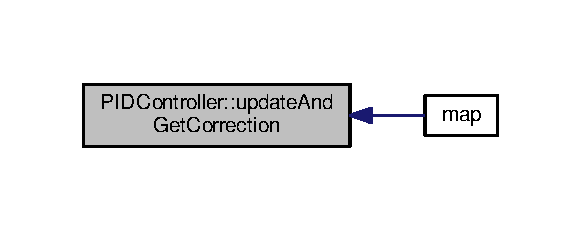
\includegraphics[width=279pt]{class_p_i_d_controller_a7cf1348b52906221761682f697902ad3_icgraph}
\end{center}
\end{figure}




The documentation for this class was generated from the following files\+:\begin{DoxyCompactItemize}
\item 
/home/travis/build/\+Autonomous-\/\+Racing-\/\+P\+G/ros.\+package/docs/master/ros\+\_\+ws/src/autonomous/include/\hyperlink{pid__controller_8h}{pid\+\_\+controller.\+h}\item 
/home/travis/build/\+Autonomous-\/\+Racing-\/\+P\+G/ros.\+package/docs/master/ros\+\_\+ws/src/autonomous/src/\hyperlink{pid__controller_8cpp}{pid\+\_\+controller.\+cpp}\end{DoxyCompactItemize}

\hypertarget{classdrive_1_1_q_learning_driving_node}{}\section{drive.\+Q\+Learning\+Driving\+Node Class Reference}
\label{classdrive_1_1_q_learning_driving_node}\index{drive.\+Q\+Learning\+Driving\+Node@{drive.\+Q\+Learning\+Driving\+Node}}


Inheritance diagram for drive.\+Q\+Learning\+Driving\+Node\+:
\nopagebreak
\begin{figure}[H]
\begin{center}
\leavevmode
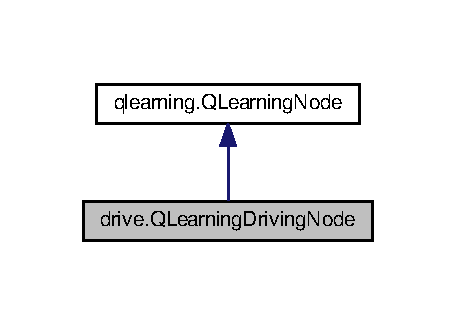
\includegraphics[width=219pt]{classdrive_1_1_q_learning_driving_node__inherit__graph}
\end{center}
\end{figure}


Collaboration diagram for drive.\+Q\+Learning\+Driving\+Node\+:
\nopagebreak
\begin{figure}[H]
\begin{center}
\leavevmode
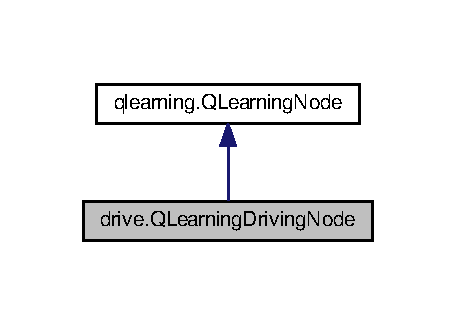
\includegraphics[width=219pt]{classdrive_1_1_q_learning_driving_node__coll__graph}
\end{center}
\end{figure}
\subsection*{Public Member Functions}
\begin{DoxyCompactItemize}
\item 
def \hyperlink{classdrive_1_1_q_learning_driving_node_ae5291b24979a8decaa85d574a20d7661}{\+\_\+\+\_\+init\+\_\+\+\_\+} (self)
\item 
def \hyperlink{classdrive_1_1_q_learning_driving_node_a2235c596e4d1f3f8d3c535abe2a1af2c}{on\+\_\+receive\+\_\+laser\+\_\+scan} (self, message)
\end{DoxyCompactItemize}
\subsection*{Additional Inherited Members}


\subsection{Detailed Description}


Definition at line 10 of file drive.\+py.



\subsection{Constructor \& Destructor Documentation}
\index{drive\+::\+Q\+Learning\+Driving\+Node@{drive\+::\+Q\+Learning\+Driving\+Node}!\+\_\+\+\_\+init\+\_\+\+\_\+@{\+\_\+\+\_\+init\+\_\+\+\_\+}}
\index{\+\_\+\+\_\+init\+\_\+\+\_\+@{\+\_\+\+\_\+init\+\_\+\+\_\+}!drive\+::\+Q\+Learning\+Driving\+Node@{drive\+::\+Q\+Learning\+Driving\+Node}}
\subsubsection[{\texorpdfstring{\+\_\+\+\_\+init\+\_\+\+\_\+(self)}{__init__(self)}}]{\setlength{\rightskip}{0pt plus 5cm}def drive.\+Q\+Learning\+Driving\+Node.\+\_\+\+\_\+init\+\_\+\+\_\+ (
\begin{DoxyParamCaption}
\item[{}]{self}
\end{DoxyParamCaption}
)}\hypertarget{classdrive_1_1_q_learning_driving_node_ae5291b24979a8decaa85d574a20d7661}{}\label{classdrive_1_1_q_learning_driving_node_ae5291b24979a8decaa85d574a20d7661}


Definition at line 11 of file drive.\+py.



\subsection{Member Function Documentation}
\index{drive\+::\+Q\+Learning\+Driving\+Node@{drive\+::\+Q\+Learning\+Driving\+Node}!on\+\_\+receive\+\_\+laser\+\_\+scan@{on\+\_\+receive\+\_\+laser\+\_\+scan}}
\index{on\+\_\+receive\+\_\+laser\+\_\+scan@{on\+\_\+receive\+\_\+laser\+\_\+scan}!drive\+::\+Q\+Learning\+Driving\+Node@{drive\+::\+Q\+Learning\+Driving\+Node}}
\subsubsection[{\texorpdfstring{on\+\_\+receive\+\_\+laser\+\_\+scan(self, message)}{on_receive_laser_scan(self, message)}}]{\setlength{\rightskip}{0pt plus 5cm}def drive.\+Q\+Learning\+Driving\+Node.\+on\+\_\+receive\+\_\+laser\+\_\+scan (
\begin{DoxyParamCaption}
\item[{}]{self, }
\item[{}]{message}
\end{DoxyParamCaption}
)}\hypertarget{classdrive_1_1_q_learning_driving_node_a2235c596e4d1f3f8d3c535abe2a1af2c}{}\label{classdrive_1_1_q_learning_driving_node_a2235c596e4d1f3f8d3c535abe2a1af2c}


Definition at line 22 of file drive.\+py.



Here is the call graph for this function\+:
\nopagebreak
\begin{figure}[H]
\begin{center}
\leavevmode
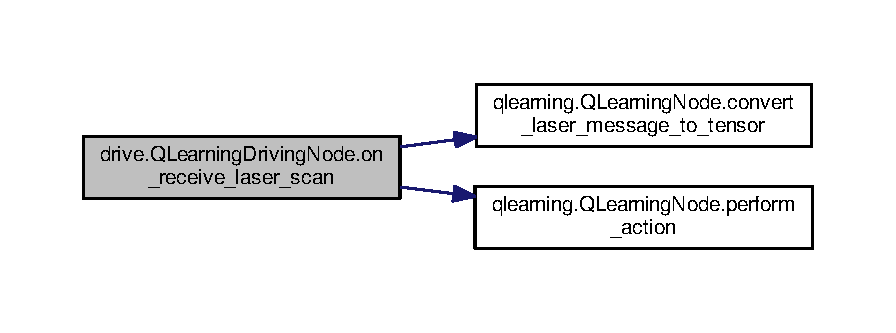
\includegraphics[width=350pt]{classdrive_1_1_q_learning_driving_node_a2235c596e4d1f3f8d3c535abe2a1af2c_cgraph}
\end{center}
\end{figure}




The documentation for this class was generated from the following file\+:\begin{DoxyCompactItemize}
\item 
/home/travis/build/\+Autonomous-\/\+Racing-\/\+P\+G/ar-\/tu-\/do/docs/master/ros\+\_\+ws/src/autonomous/reinforcement\+\_\+learning/scripts/\hyperlink{drive_8py}{drive.\+py}\end{DoxyCompactItemize}

\hypertarget{classqlearning_1_1_q_learning_node}{}\section{qlearning.\+Q\+Learning\+Node Class Reference}
\label{classqlearning_1_1_q_learning_node}\index{qlearning.\+Q\+Learning\+Node@{qlearning.\+Q\+Learning\+Node}}


Inheritance diagram for qlearning.\+Q\+Learning\+Node\+:
\nopagebreak
\begin{figure}[H]
\begin{center}
\leavevmode
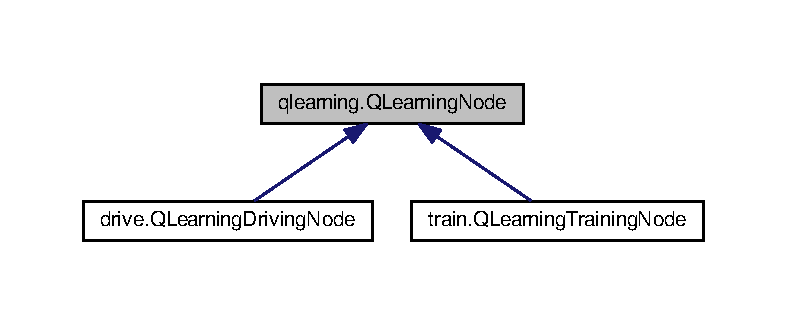
\includegraphics[width=350pt]{classqlearning_1_1_q_learning_node__inherit__graph}
\end{center}
\end{figure}
\subsection*{Public Member Functions}
\begin{DoxyCompactItemize}
\item 
def \hyperlink{classqlearning_1_1_q_learning_node_a6f95c46edee5acba7c59a3eac4e04a2a}{\+\_\+\+\_\+init\+\_\+\+\_\+} (self)
\item 
def \hyperlink{classqlearning_1_1_q_learning_node_a70f975497db6b5eee94485397b7c18e6}{perform\+\_\+action} (self, action\+\_\+index)
\item 
def \hyperlink{classqlearning_1_1_q_learning_node_a907441bbc5b795875ea80de4a6b45798}{convert\+\_\+laser\+\_\+message\+\_\+to\+\_\+tensor} (self, message)
\item 
def \hyperlink{classqlearning_1_1_q_learning_node_a2ac97685465b2c7d22ca26019cf2fff5}{on\+\_\+receive\+\_\+laser\+\_\+scan} (self, message)
\end{DoxyCompactItemize}
\subsection*{Public Attributes}
\begin{DoxyCompactItemize}
\item 
\hyperlink{classqlearning_1_1_q_learning_node_a2c1150dd506209b085dad03036775375}{policy}
\item 
\hyperlink{classqlearning_1_1_q_learning_node_a40b085aff23685cc49b297f287743ed6}{scan\+\_\+indices}
\item 
\hyperlink{classqlearning_1_1_q_learning_node_a2885dd3e3dbd44c0627829d35f9e0041}{drive\+\_\+parameters\+\_\+publisher}
\end{DoxyCompactItemize}


\subsection{Detailed Description}


Definition at line 13 of file qlearning.\+py.



\subsection{Constructor \& Destructor Documentation}
\index{qlearning\+::\+Q\+Learning\+Node@{qlearning\+::\+Q\+Learning\+Node}!\+\_\+\+\_\+init\+\_\+\+\_\+@{\+\_\+\+\_\+init\+\_\+\+\_\+}}
\index{\+\_\+\+\_\+init\+\_\+\+\_\+@{\+\_\+\+\_\+init\+\_\+\+\_\+}!qlearning\+::\+Q\+Learning\+Node@{qlearning\+::\+Q\+Learning\+Node}}
\subsubsection[{\texorpdfstring{\+\_\+\+\_\+init\+\_\+\+\_\+(self)}{__init__(self)}}]{\setlength{\rightskip}{0pt plus 5cm}def qlearning.\+Q\+Learning\+Node.\+\_\+\+\_\+init\+\_\+\+\_\+ (
\begin{DoxyParamCaption}
\item[{}]{self}
\end{DoxyParamCaption}
)}\hypertarget{classqlearning_1_1_q_learning_node_a6f95c46edee5acba7c59a3eac4e04a2a}{}\label{classqlearning_1_1_q_learning_node_a6f95c46edee5acba7c59a3eac4e04a2a}


Definition at line 14 of file qlearning.\+py.



\subsection{Member Function Documentation}
\index{qlearning\+::\+Q\+Learning\+Node@{qlearning\+::\+Q\+Learning\+Node}!convert\+\_\+laser\+\_\+message\+\_\+to\+\_\+tensor@{convert\+\_\+laser\+\_\+message\+\_\+to\+\_\+tensor}}
\index{convert\+\_\+laser\+\_\+message\+\_\+to\+\_\+tensor@{convert\+\_\+laser\+\_\+message\+\_\+to\+\_\+tensor}!qlearning\+::\+Q\+Learning\+Node@{qlearning\+::\+Q\+Learning\+Node}}
\subsubsection[{\texorpdfstring{convert\+\_\+laser\+\_\+message\+\_\+to\+\_\+tensor(self, message)}{convert_laser_message_to_tensor(self, message)}}]{\setlength{\rightskip}{0pt plus 5cm}def qlearning.\+Q\+Learning\+Node.\+convert\+\_\+laser\+\_\+message\+\_\+to\+\_\+tensor (
\begin{DoxyParamCaption}
\item[{}]{self, }
\item[{}]{message}
\end{DoxyParamCaption}
)}\hypertarget{classqlearning_1_1_q_learning_node_a907441bbc5b795875ea80de4a6b45798}{}\label{classqlearning_1_1_q_learning_node_a907441bbc5b795875ea80de4a6b45798}


Definition at line 32 of file qlearning.\+py.



Here is the caller graph for this function\+:
\nopagebreak
\begin{figure}[H]
\begin{center}
\leavevmode
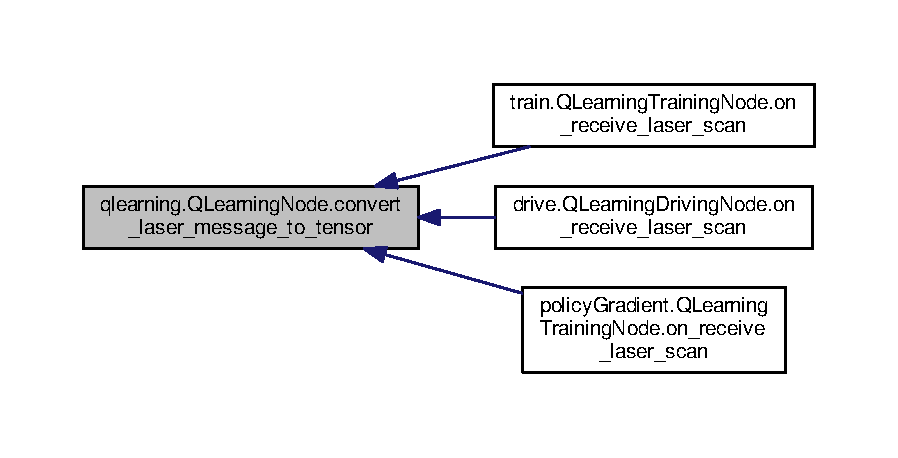
\includegraphics[width=350pt]{classqlearning_1_1_q_learning_node_a907441bbc5b795875ea80de4a6b45798_icgraph}
\end{center}
\end{figure}


\index{qlearning\+::\+Q\+Learning\+Node@{qlearning\+::\+Q\+Learning\+Node}!on\+\_\+receive\+\_\+laser\+\_\+scan@{on\+\_\+receive\+\_\+laser\+\_\+scan}}
\index{on\+\_\+receive\+\_\+laser\+\_\+scan@{on\+\_\+receive\+\_\+laser\+\_\+scan}!qlearning\+::\+Q\+Learning\+Node@{qlearning\+::\+Q\+Learning\+Node}}
\subsubsection[{\texorpdfstring{on\+\_\+receive\+\_\+laser\+\_\+scan(self, message)}{on_receive_laser_scan(self, message)}}]{\setlength{\rightskip}{0pt plus 5cm}def qlearning.\+Q\+Learning\+Node.\+on\+\_\+receive\+\_\+laser\+\_\+scan (
\begin{DoxyParamCaption}
\item[{}]{self, }
\item[{}]{message}
\end{DoxyParamCaption}
)}\hypertarget{classqlearning_1_1_q_learning_node_a2ac97685465b2c7d22ca26019cf2fff5}{}\label{classqlearning_1_1_q_learning_node_a2ac97685465b2c7d22ca26019cf2fff5}


Definition at line 44 of file qlearning.\+py.

\index{qlearning\+::\+Q\+Learning\+Node@{qlearning\+::\+Q\+Learning\+Node}!perform\+\_\+action@{perform\+\_\+action}}
\index{perform\+\_\+action@{perform\+\_\+action}!qlearning\+::\+Q\+Learning\+Node@{qlearning\+::\+Q\+Learning\+Node}}
\subsubsection[{\texorpdfstring{perform\+\_\+action(self, action\+\_\+index)}{perform_action(self, action_index)}}]{\setlength{\rightskip}{0pt plus 5cm}def qlearning.\+Q\+Learning\+Node.\+perform\+\_\+action (
\begin{DoxyParamCaption}
\item[{}]{self, }
\item[{}]{action\+\_\+index}
\end{DoxyParamCaption}
)}\hypertarget{classqlearning_1_1_q_learning_node_a70f975497db6b5eee94485397b7c18e6}{}\label{classqlearning_1_1_q_learning_node_a70f975497db6b5eee94485397b7c18e6}


Definition at line 22 of file qlearning.\+py.



Here is the caller graph for this function\+:
\nopagebreak
\begin{figure}[H]
\begin{center}
\leavevmode
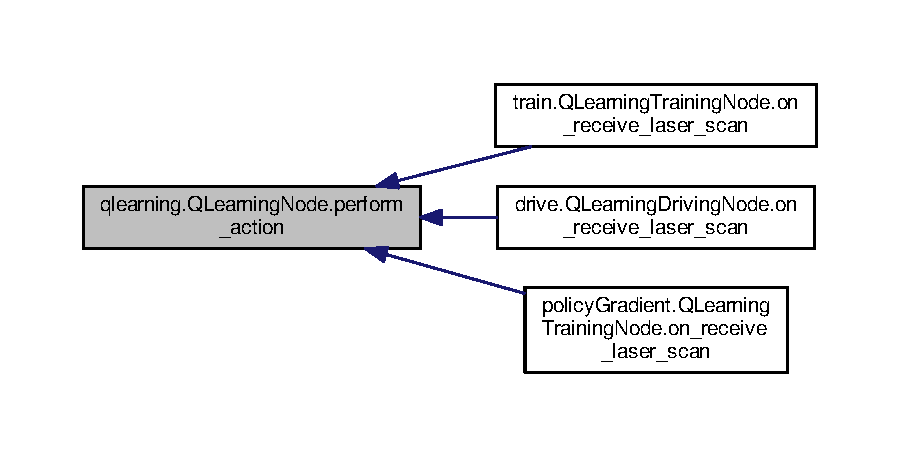
\includegraphics[width=350pt]{classqlearning_1_1_q_learning_node_a70f975497db6b5eee94485397b7c18e6_icgraph}
\end{center}
\end{figure}




\subsection{Member Data Documentation}
\index{qlearning\+::\+Q\+Learning\+Node@{qlearning\+::\+Q\+Learning\+Node}!drive\+\_\+parameters\+\_\+publisher@{drive\+\_\+parameters\+\_\+publisher}}
\index{drive\+\_\+parameters\+\_\+publisher@{drive\+\_\+parameters\+\_\+publisher}!qlearning\+::\+Q\+Learning\+Node@{qlearning\+::\+Q\+Learning\+Node}}
\subsubsection[{\texorpdfstring{drive\+\_\+parameters\+\_\+publisher}{drive_parameters_publisher}}]{\setlength{\rightskip}{0pt plus 5cm}qlearning.\+Q\+Learning\+Node.\+drive\+\_\+parameters\+\_\+publisher}\hypertarget{classqlearning_1_1_q_learning_node_a2885dd3e3dbd44c0627829d35f9e0041}{}\label{classqlearning_1_1_q_learning_node_a2885dd3e3dbd44c0627829d35f9e0041}


Definition at line 18 of file qlearning.\+py.

\index{qlearning\+::\+Q\+Learning\+Node@{qlearning\+::\+Q\+Learning\+Node}!policy@{policy}}
\index{policy@{policy}!qlearning\+::\+Q\+Learning\+Node@{qlearning\+::\+Q\+Learning\+Node}}
\subsubsection[{\texorpdfstring{policy}{policy}}]{\setlength{\rightskip}{0pt plus 5cm}qlearning.\+Q\+Learning\+Node.\+policy}\hypertarget{classqlearning_1_1_q_learning_node_a2c1150dd506209b085dad03036775375}{}\label{classqlearning_1_1_q_learning_node_a2c1150dd506209b085dad03036775375}


Definition at line 15 of file qlearning.\+py.

\index{qlearning\+::\+Q\+Learning\+Node@{qlearning\+::\+Q\+Learning\+Node}!scan\+\_\+indices@{scan\+\_\+indices}}
\index{scan\+\_\+indices@{scan\+\_\+indices}!qlearning\+::\+Q\+Learning\+Node@{qlearning\+::\+Q\+Learning\+Node}}
\subsubsection[{\texorpdfstring{scan\+\_\+indices}{scan_indices}}]{\setlength{\rightskip}{0pt plus 5cm}qlearning.\+Q\+Learning\+Node.\+scan\+\_\+indices}\hypertarget{classqlearning_1_1_q_learning_node_a40b085aff23685cc49b297f287743ed6}{}\label{classqlearning_1_1_q_learning_node_a40b085aff23685cc49b297f287743ed6}


Definition at line 17 of file qlearning.\+py.



The documentation for this class was generated from the following file\+:\begin{DoxyCompactItemize}
\item 
/home/travis/build/\+Autonomous-\/\+Racing-\/\+P\+G/ros.\+package/docs/master/ros\+\_\+ws/src/autonomous/q\+\_\+learning/scripts/\hyperlink{qlearning_8py}{qlearning.\+py}\end{DoxyCompactItemize}

\hypertarget{classtrain_1_1_q_learning_training_node}{}\section{train.\+Q\+Learning\+Training\+Node Class Reference}
\label{classtrain_1_1_q_learning_training_node}\index{train.\+Q\+Learning\+Training\+Node@{train.\+Q\+Learning\+Training\+Node}}


Inheritance diagram for train.\+Q\+Learning\+Training\+Node\+:
\nopagebreak
\begin{figure}[H]
\begin{center}
\leavevmode
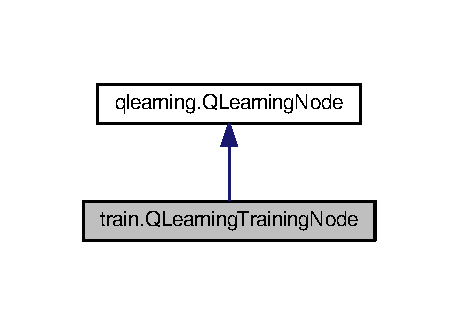
\includegraphics[width=220pt]{classtrain_1_1_q_learning_training_node__inherit__graph}
\end{center}
\end{figure}


Collaboration diagram for train.\+Q\+Learning\+Training\+Node\+:
\nopagebreak
\begin{figure}[H]
\begin{center}
\leavevmode
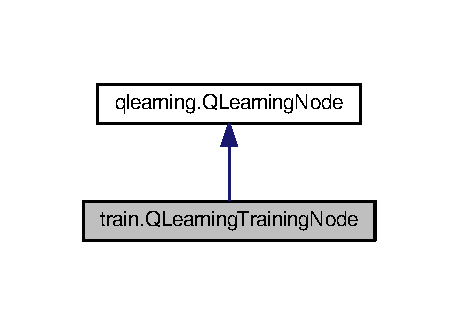
\includegraphics[width=220pt]{classtrain_1_1_q_learning_training_node__coll__graph}
\end{center}
\end{figure}
\subsection*{Public Member Functions}
\begin{DoxyCompactItemize}
\item 
def \hyperlink{classtrain_1_1_q_learning_training_node_a29b8eee27131f26d94387231e3970021}{\+\_\+\+\_\+init\+\_\+\+\_\+} (self)
\item 
def \hyperlink{classtrain_1_1_q_learning_training_node_a82007327cc0867fb55d159d2ed3568b6}{replay} (self)
\item 
def \hyperlink{classtrain_1_1_q_learning_training_node_a9f5b2be91deca2b12d3dd055ce294449}{on\+\_\+crash} (self, \+\_\+)
\item 
def \hyperlink{classtrain_1_1_q_learning_training_node_ab4d0383d228012c56c9dd31886b80df6}{get\+\_\+epsilon\+\_\+greedy\+\_\+threshold} (self)
\item 
def \hyperlink{classtrain_1_1_q_learning_training_node_ac03f4ced7d65ef3c2cf36978796fcfda}{select\+\_\+action} (self, \hyperlink{classtrain_1_1_q_learning_training_node_a6e860eb510dc030f536d26c2a3fcc33c}{state})
\item 
def \hyperlink{classtrain_1_1_q_learning_training_node_a1fea335e8f7d2eb257e97364bab331a7}{get\+\_\+reward} (self)
\item 
def \hyperlink{classtrain_1_1_q_learning_training_node_a7263bf517e3d306b383f5d30bf02e8c8}{log\+\_\+training\+\_\+progress} (self)
\item 
def \hyperlink{classtrain_1_1_q_learning_training_node_a659667f05d48676284265ee0e445e96e}{on\+\_\+complete\+\_\+episode} (self)
\item 
def \hyperlink{classtrain_1_1_q_learning_training_node_aeff9ce73821ded751c709f5f5acabd22}{check\+\_\+car\+\_\+orientation} (self)
\item 
def \hyperlink{classtrain_1_1_q_learning_training_node_a4cb5d38537fbb9171e46c85b60efc700}{on\+\_\+receive\+\_\+laser\+\_\+scan} (self, message)
\item 
def \hyperlink{classtrain_1_1_q_learning_training_node_a167547fdc06e2d452d972024fd632b9c}{on\+\_\+model\+\_\+state\+\_\+callback} (self, message)
\end{DoxyCompactItemize}
\subsection*{Public Attributes}
\begin{DoxyCompactItemize}
\item 
\hyperlink{classtrain_1_1_q_learning_training_node_a5bef341c2aa0b019a190efb961701cdc}{episode\+\_\+count}
\item 
\hyperlink{classtrain_1_1_q_learning_training_node_abaa1cd9793d6724977d7b9451e36bc3b}{episode\+\_\+length}
\item 
\hyperlink{classtrain_1_1_q_learning_training_node_aa583fe782e5ae47cc64dd44b92fd2e71}{total\+\_\+step\+\_\+count}
\item 
\hyperlink{classtrain_1_1_q_learning_training_node_a876c1cedd4eabcca4e9a0ee6e0922752}{optimization\+\_\+step\+\_\+count}
\item 
\hyperlink{classtrain_1_1_q_learning_training_node_a4c632e44085797e564501bba836b7359}{cumulative\+\_\+reward}
\item 
\hyperlink{classtrain_1_1_q_learning_training_node_a0f8d5e71ae52a959d5248f57ac55829a}{is\+\_\+terminal\+\_\+step}
\item 
\hyperlink{classtrain_1_1_q_learning_training_node_a5837c478232e1d4cc646bfbadbdd2ff2}{net\+\_\+output\+\_\+debug\+\_\+string}
\item 
\hyperlink{classtrain_1_1_q_learning_training_node_af81cfd1d0306828d0ff901faf85df6b3}{episode\+\_\+length\+\_\+history}
\item 
\hyperlink{classtrain_1_1_q_learning_training_node_aa25b9712eebb6aed6befa421814472b4}{cumulative\+\_\+reward\+\_\+history}
\item 
\hyperlink{classtrain_1_1_q_learning_training_node_a6e860eb510dc030f536d26c2a3fcc33c}{state}
\item 
\hyperlink{classtrain_1_1_q_learning_training_node_ad42c35a16230d89d787b5a3a74808edf}{action}
\item 
\hyperlink{classtrain_1_1_q_learning_training_node_ac802eca257307ce6c83897c612aa5f90}{car\+\_\+position}
\item 
\hyperlink{classtrain_1_1_q_learning_training_node_a016d2adc85428e64903703974f8cd79c}{car\+\_\+orientation}
\item 
\hyperlink{classtrain_1_1_q_learning_training_node_a400f047c3086a321f255b2405f2ebe1f}{drive\+\_\+forward}
\item 
\hyperlink{classtrain_1_1_q_learning_training_node_a87a28e543665823ac18758f6a4460d7a}{steps\+\_\+with\+\_\+wrong\+\_\+orientation}
\item 
\hyperlink{classtrain_1_1_q_learning_training_node_a407532bec47855fec93201fa87fe80ab}{real\+\_\+time\+\_\+factor}
\item 
\hyperlink{classtrain_1_1_q_learning_training_node_a8efbf39c7dcf595fb7c02121c66f9f53}{episode\+\_\+start\+\_\+time\+\_\+real}
\item 
\hyperlink{classtrain_1_1_q_learning_training_node_aaba249fe751adb0b4167b350ee2ea7a1}{episode\+\_\+start\+\_\+time\+\_\+sim}
\item 
\hyperlink{classtrain_1_1_q_learning_training_node_a2cd6ba599812ec0edffba7869f4f27d9}{optimizer}
\item 
\hyperlink{classtrain_1_1_q_learning_training_node_a49440485cce2f2f3fe9575456a562098}{memory}
\item 
\hyperlink{classtrain_1_1_q_learning_training_node_a7fef779ba6b1592b9ed2837abe5ae6ae}{episode\+\_\+result\+\_\+publisher}
\end{DoxyCompactItemize}


\subsection{Detailed Description}


Definition at line 26 of file train.\+py.



\subsection{Constructor \& Destructor Documentation}
\index{train\+::\+Q\+Learning\+Training\+Node@{train\+::\+Q\+Learning\+Training\+Node}!\+\_\+\+\_\+init\+\_\+\+\_\+@{\+\_\+\+\_\+init\+\_\+\+\_\+}}
\index{\+\_\+\+\_\+init\+\_\+\+\_\+@{\+\_\+\+\_\+init\+\_\+\+\_\+}!train\+::\+Q\+Learning\+Training\+Node@{train\+::\+Q\+Learning\+Training\+Node}}
\subsubsection[{\texorpdfstring{\+\_\+\+\_\+init\+\_\+\+\_\+(self)}{__init__(self)}}]{\setlength{\rightskip}{0pt plus 5cm}def train.\+Q\+Learning\+Training\+Node.\+\_\+\+\_\+init\+\_\+\+\_\+ (
\begin{DoxyParamCaption}
\item[{}]{self}
\end{DoxyParamCaption}
)}\hypertarget{classtrain_1_1_q_learning_training_node_a29b8eee27131f26d94387231e3970021}{}\label{classtrain_1_1_q_learning_training_node_a29b8eee27131f26d94387231e3970021}


Definition at line 27 of file train.\+py.



\subsection{Member Function Documentation}
\index{train\+::\+Q\+Learning\+Training\+Node@{train\+::\+Q\+Learning\+Training\+Node}!check\+\_\+car\+\_\+orientation@{check\+\_\+car\+\_\+orientation}}
\index{check\+\_\+car\+\_\+orientation@{check\+\_\+car\+\_\+orientation}!train\+::\+Q\+Learning\+Training\+Node@{train\+::\+Q\+Learning\+Training\+Node}}
\subsubsection[{\texorpdfstring{check\+\_\+car\+\_\+orientation(self)}{check_car_orientation(self)}}]{\setlength{\rightskip}{0pt plus 5cm}def train.\+Q\+Learning\+Training\+Node.\+check\+\_\+car\+\_\+orientation (
\begin{DoxyParamCaption}
\item[{}]{self}
\end{DoxyParamCaption}
)}\hypertarget{classtrain_1_1_q_learning_training_node_aeff9ce73821ded751c709f5f5acabd22}{}\label{classtrain_1_1_q_learning_training_node_aeff9ce73821ded751c709f5f5acabd22}


Definition at line 166 of file train.\+py.



Here is the caller graph for this function\+:
\nopagebreak
\begin{figure}[H]
\begin{center}
\leavevmode
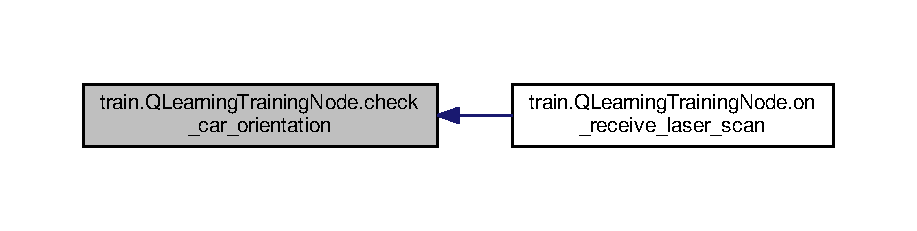
\includegraphics[width=350pt]{classtrain_1_1_q_learning_training_node_aeff9ce73821ded751c709f5f5acabd22_icgraph}
\end{center}
\end{figure}


\index{train\+::\+Q\+Learning\+Training\+Node@{train\+::\+Q\+Learning\+Training\+Node}!get\+\_\+epsilon\+\_\+greedy\+\_\+threshold@{get\+\_\+epsilon\+\_\+greedy\+\_\+threshold}}
\index{get\+\_\+epsilon\+\_\+greedy\+\_\+threshold@{get\+\_\+epsilon\+\_\+greedy\+\_\+threshold}!train\+::\+Q\+Learning\+Training\+Node@{train\+::\+Q\+Learning\+Training\+Node}}
\subsubsection[{\texorpdfstring{get\+\_\+epsilon\+\_\+greedy\+\_\+threshold(self)}{get_epsilon_greedy_threshold(self)}}]{\setlength{\rightskip}{0pt plus 5cm}def train.\+Q\+Learning\+Training\+Node.\+get\+\_\+epsilon\+\_\+greedy\+\_\+threshold (
\begin{DoxyParamCaption}
\item[{}]{self}
\end{DoxyParamCaption}
)}\hypertarget{classtrain_1_1_q_learning_training_node_ab4d0383d228012c56c9dd31886b80df6}{}\label{classtrain_1_1_q_learning_training_node_ab4d0383d228012c56c9dd31886b80df6}


Definition at line 100 of file train.\+py.



Here is the caller graph for this function\+:
\nopagebreak
\begin{figure}[H]
\begin{center}
\leavevmode
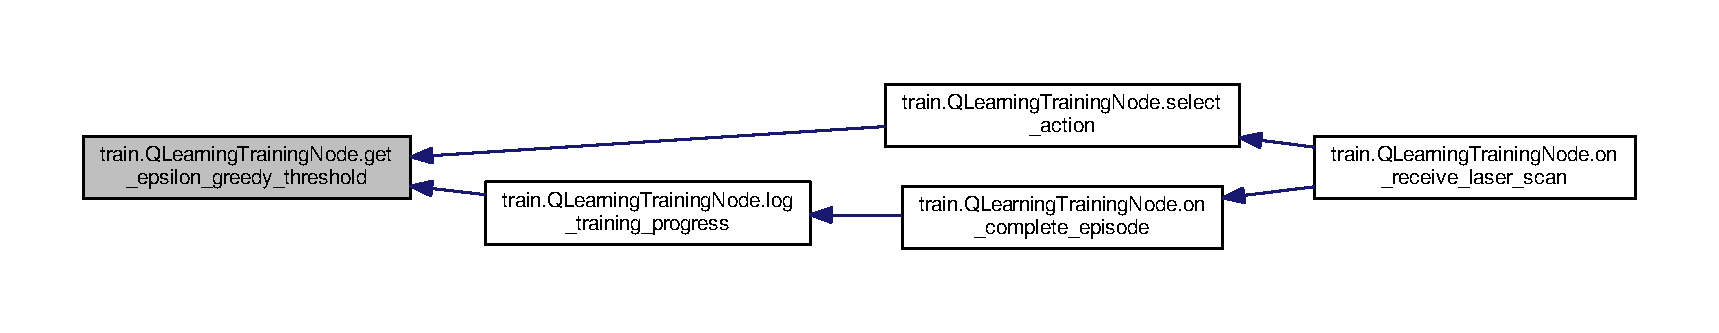
\includegraphics[width=350pt]{classtrain_1_1_q_learning_training_node_ab4d0383d228012c56c9dd31886b80df6_icgraph}
\end{center}
\end{figure}


\index{train\+::\+Q\+Learning\+Training\+Node@{train\+::\+Q\+Learning\+Training\+Node}!get\+\_\+reward@{get\+\_\+reward}}
\index{get\+\_\+reward@{get\+\_\+reward}!train\+::\+Q\+Learning\+Training\+Node@{train\+::\+Q\+Learning\+Training\+Node}}
\subsubsection[{\texorpdfstring{get\+\_\+reward(self)}{get_reward(self)}}]{\setlength{\rightskip}{0pt plus 5cm}def train.\+Q\+Learning\+Training\+Node.\+get\+\_\+reward (
\begin{DoxyParamCaption}
\item[{}]{self}
\end{DoxyParamCaption}
)}\hypertarget{classtrain_1_1_q_learning_training_node_a1fea335e8f7d2eb257e97364bab331a7}{}\label{classtrain_1_1_q_learning_training_node_a1fea335e8f7d2eb257e97364bab331a7}


Definition at line 116 of file train.\+py.



Here is the caller graph for this function\+:
\nopagebreak
\begin{figure}[H]
\begin{center}
\leavevmode
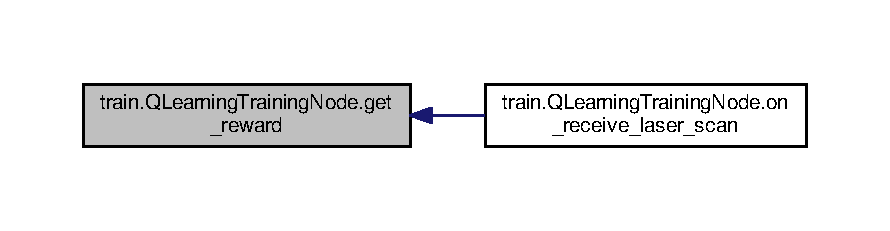
\includegraphics[width=350pt]{classtrain_1_1_q_learning_training_node_a1fea335e8f7d2eb257e97364bab331a7_icgraph}
\end{center}
\end{figure}


\index{train\+::\+Q\+Learning\+Training\+Node@{train\+::\+Q\+Learning\+Training\+Node}!log\+\_\+training\+\_\+progress@{log\+\_\+training\+\_\+progress}}
\index{log\+\_\+training\+\_\+progress@{log\+\_\+training\+\_\+progress}!train\+::\+Q\+Learning\+Training\+Node@{train\+::\+Q\+Learning\+Training\+Node}}
\subsubsection[{\texorpdfstring{log\+\_\+training\+\_\+progress(self)}{log_training_progress(self)}}]{\setlength{\rightskip}{0pt plus 5cm}def train.\+Q\+Learning\+Training\+Node.\+log\+\_\+training\+\_\+progress (
\begin{DoxyParamCaption}
\item[{}]{self}
\end{DoxyParamCaption}
)}\hypertarget{classtrain_1_1_q_learning_training_node_a7263bf517e3d306b383f5d30bf02e8c8}{}\label{classtrain_1_1_q_learning_training_node_a7263bf517e3d306b383f5d30bf02e8c8}


Definition at line 127 of file train.\+py.



Here is the call graph for this function\+:
\nopagebreak
\begin{figure}[H]
\begin{center}
\leavevmode
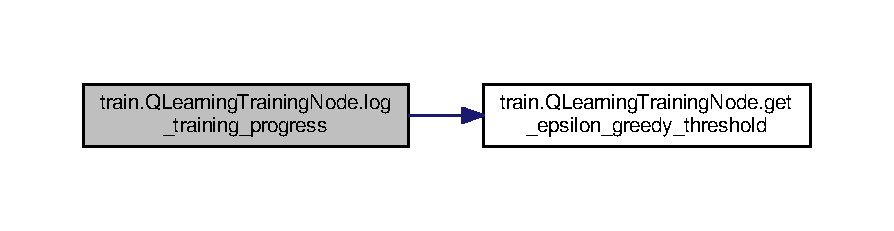
\includegraphics[width=350pt]{classtrain_1_1_q_learning_training_node_a7263bf517e3d306b383f5d30bf02e8c8_cgraph}
\end{center}
\end{figure}




Here is the caller graph for this function\+:
\nopagebreak
\begin{figure}[H]
\begin{center}
\leavevmode
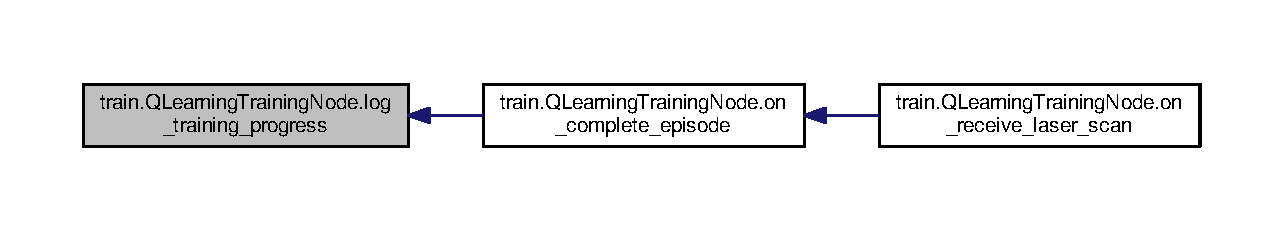
\includegraphics[width=350pt]{classtrain_1_1_q_learning_training_node_a7263bf517e3d306b383f5d30bf02e8c8_icgraph}
\end{center}
\end{figure}


\index{train\+::\+Q\+Learning\+Training\+Node@{train\+::\+Q\+Learning\+Training\+Node}!on\+\_\+complete\+\_\+episode@{on\+\_\+complete\+\_\+episode}}
\index{on\+\_\+complete\+\_\+episode@{on\+\_\+complete\+\_\+episode}!train\+::\+Q\+Learning\+Training\+Node@{train\+::\+Q\+Learning\+Training\+Node}}
\subsubsection[{\texorpdfstring{on\+\_\+complete\+\_\+episode(self)}{on_complete_episode(self)}}]{\setlength{\rightskip}{0pt plus 5cm}def train.\+Q\+Learning\+Training\+Node.\+on\+\_\+complete\+\_\+episode (
\begin{DoxyParamCaption}
\item[{}]{self}
\end{DoxyParamCaption}
)}\hypertarget{classtrain_1_1_q_learning_training_node_a659667f05d48676284265ee0e445e96e}{}\label{classtrain_1_1_q_learning_training_node_a659667f05d48676284265ee0e445e96e}


Definition at line 144 of file train.\+py.



Here is the call graph for this function\+:
\nopagebreak
\begin{figure}[H]
\begin{center}
\leavevmode
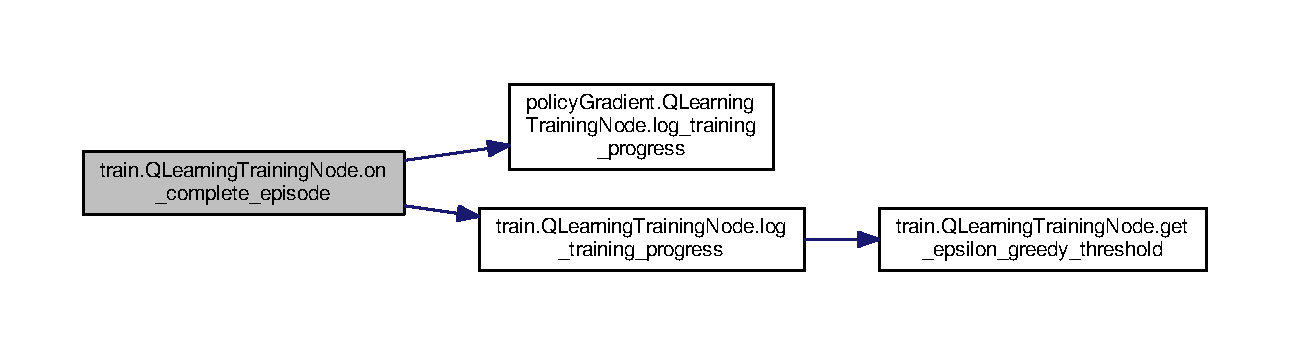
\includegraphics[width=350pt]{classtrain_1_1_q_learning_training_node_a659667f05d48676284265ee0e445e96e_cgraph}
\end{center}
\end{figure}




Here is the caller graph for this function\+:
\nopagebreak
\begin{figure}[H]
\begin{center}
\leavevmode
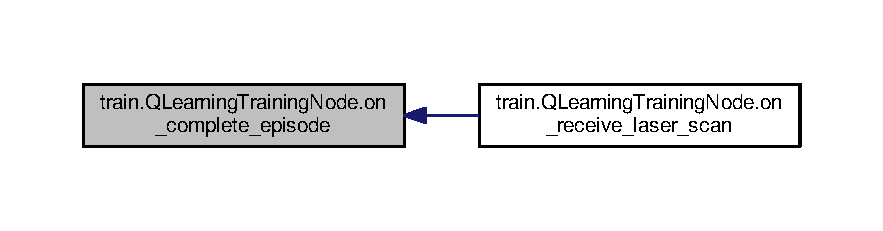
\includegraphics[width=350pt]{classtrain_1_1_q_learning_training_node_a659667f05d48676284265ee0e445e96e_icgraph}
\end{center}
\end{figure}


\index{train\+::\+Q\+Learning\+Training\+Node@{train\+::\+Q\+Learning\+Training\+Node}!on\+\_\+crash@{on\+\_\+crash}}
\index{on\+\_\+crash@{on\+\_\+crash}!train\+::\+Q\+Learning\+Training\+Node@{train\+::\+Q\+Learning\+Training\+Node}}
\subsubsection[{\texorpdfstring{on\+\_\+crash(self, \+\_\+)}{on_crash(self, _)}}]{\setlength{\rightskip}{0pt plus 5cm}def train.\+Q\+Learning\+Training\+Node.\+on\+\_\+crash (
\begin{DoxyParamCaption}
\item[{}]{self, }
\item[{}]{\+\_\+}
\end{DoxyParamCaption}
)}\hypertarget{classtrain_1_1_q_learning_training_node_a9f5b2be91deca2b12d3dd055ce294449}{}\label{classtrain_1_1_q_learning_training_node_a9f5b2be91deca2b12d3dd055ce294449}


Definition at line 96 of file train.\+py.

\index{train\+::\+Q\+Learning\+Training\+Node@{train\+::\+Q\+Learning\+Training\+Node}!on\+\_\+model\+\_\+state\+\_\+callback@{on\+\_\+model\+\_\+state\+\_\+callback}}
\index{on\+\_\+model\+\_\+state\+\_\+callback@{on\+\_\+model\+\_\+state\+\_\+callback}!train\+::\+Q\+Learning\+Training\+Node@{train\+::\+Q\+Learning\+Training\+Node}}
\subsubsection[{\texorpdfstring{on\+\_\+model\+\_\+state\+\_\+callback(self, message)}{on_model_state_callback(self, message)}}]{\setlength{\rightskip}{0pt plus 5cm}def train.\+Q\+Learning\+Training\+Node.\+on\+\_\+model\+\_\+state\+\_\+callback (
\begin{DoxyParamCaption}
\item[{}]{self, }
\item[{}]{message}
\end{DoxyParamCaption}
)}\hypertarget{classtrain_1_1_q_learning_training_node_a167547fdc06e2d452d972024fd632b9c}{}\label{classtrain_1_1_q_learning_training_node_a167547fdc06e2d452d972024fd632b9c}


Definition at line 207 of file train.\+py.

\index{train\+::\+Q\+Learning\+Training\+Node@{train\+::\+Q\+Learning\+Training\+Node}!on\+\_\+receive\+\_\+laser\+\_\+scan@{on\+\_\+receive\+\_\+laser\+\_\+scan}}
\index{on\+\_\+receive\+\_\+laser\+\_\+scan@{on\+\_\+receive\+\_\+laser\+\_\+scan}!train\+::\+Q\+Learning\+Training\+Node@{train\+::\+Q\+Learning\+Training\+Node}}
\subsubsection[{\texorpdfstring{on\+\_\+receive\+\_\+laser\+\_\+scan(self, message)}{on_receive_laser_scan(self, message)}}]{\setlength{\rightskip}{0pt plus 5cm}def train.\+Q\+Learning\+Training\+Node.\+on\+\_\+receive\+\_\+laser\+\_\+scan (
\begin{DoxyParamCaption}
\item[{}]{self, }
\item[{}]{message}
\end{DoxyParamCaption}
)}\hypertarget{classtrain_1_1_q_learning_training_node_a4cb5d38537fbb9171e46c85b60efc700}{}\label{classtrain_1_1_q_learning_training_node_a4cb5d38537fbb9171e46c85b60efc700}


Definition at line 180 of file train.\+py.



Here is the call graph for this function\+:
\nopagebreak
\begin{figure}[H]
\begin{center}
\leavevmode
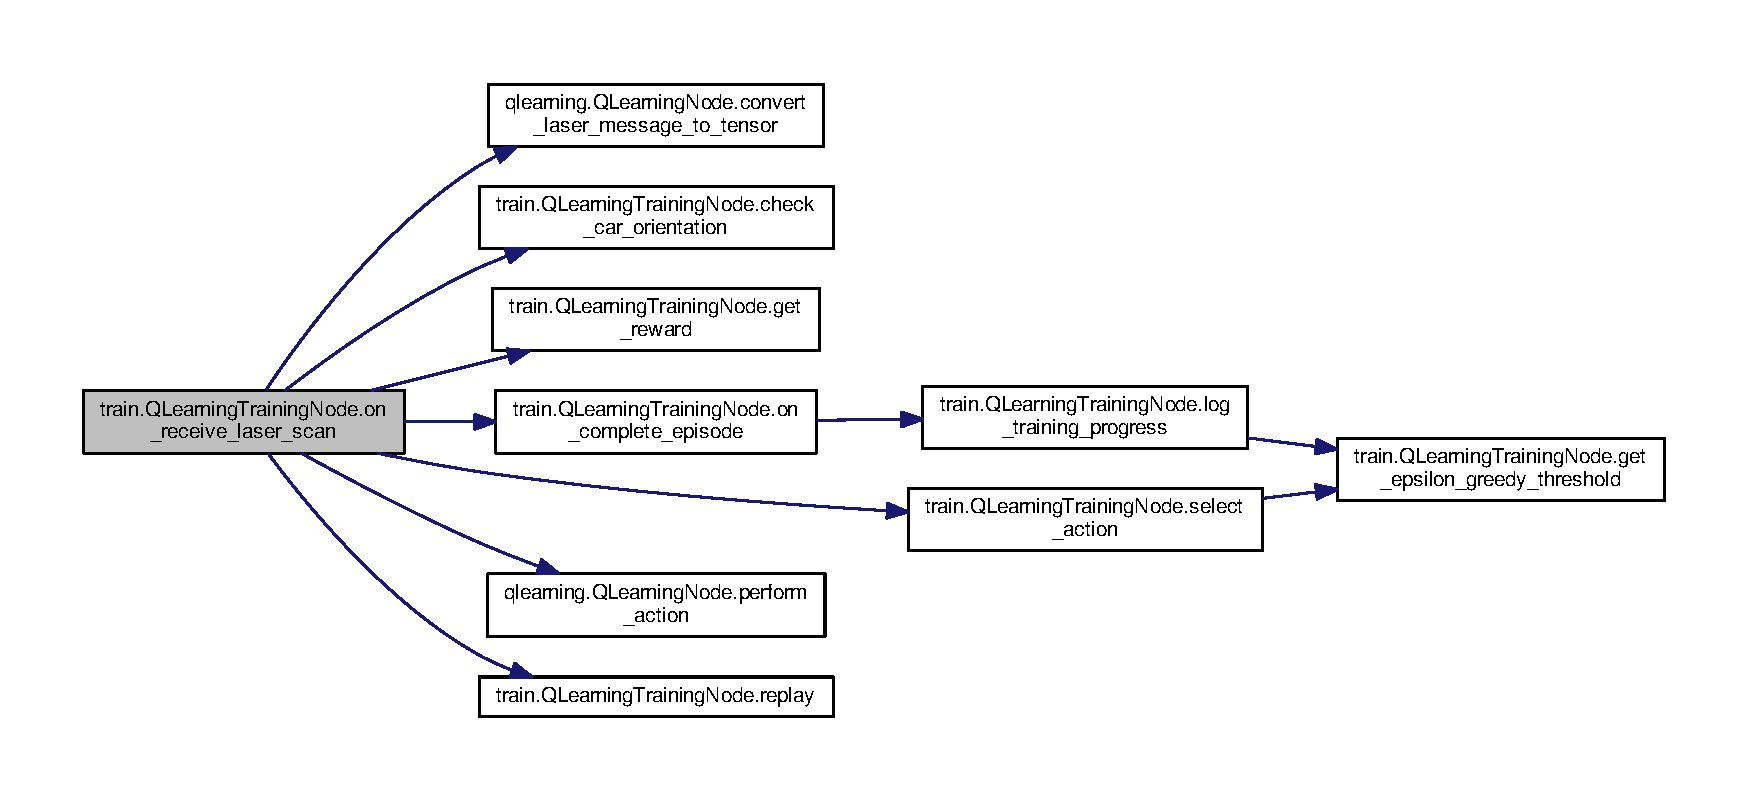
\includegraphics[width=350pt]{classtrain_1_1_q_learning_training_node_a4cb5d38537fbb9171e46c85b60efc700_cgraph}
\end{center}
\end{figure}


\index{train\+::\+Q\+Learning\+Training\+Node@{train\+::\+Q\+Learning\+Training\+Node}!replay@{replay}}
\index{replay@{replay}!train\+::\+Q\+Learning\+Training\+Node@{train\+::\+Q\+Learning\+Training\+Node}}
\subsubsection[{\texorpdfstring{replay(self)}{replay(self)}}]{\setlength{\rightskip}{0pt plus 5cm}def train.\+Q\+Learning\+Training\+Node.\+replay (
\begin{DoxyParamCaption}
\item[{}]{self}
\end{DoxyParamCaption}
)}\hypertarget{classtrain_1_1_q_learning_training_node_a82007327cc0867fb55d159d2ed3568b6}{}\label{classtrain_1_1_q_learning_training_node_a82007327cc0867fb55d159d2ed3568b6}


Definition at line 66 of file train.\+py.



Here is the caller graph for this function\+:
\nopagebreak
\begin{figure}[H]
\begin{center}
\leavevmode
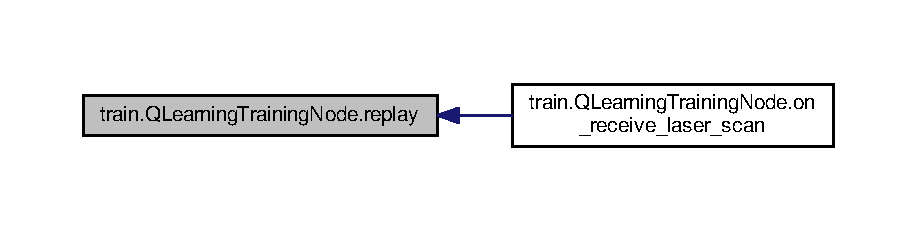
\includegraphics[width=350pt]{classtrain_1_1_q_learning_training_node_a82007327cc0867fb55d159d2ed3568b6_icgraph}
\end{center}
\end{figure}


\index{train\+::\+Q\+Learning\+Training\+Node@{train\+::\+Q\+Learning\+Training\+Node}!select\+\_\+action@{select\+\_\+action}}
\index{select\+\_\+action@{select\+\_\+action}!train\+::\+Q\+Learning\+Training\+Node@{train\+::\+Q\+Learning\+Training\+Node}}
\subsubsection[{\texorpdfstring{select\+\_\+action(self, state)}{select_action(self, state)}}]{\setlength{\rightskip}{0pt plus 5cm}def train.\+Q\+Learning\+Training\+Node.\+select\+\_\+action (
\begin{DoxyParamCaption}
\item[{}]{self, }
\item[{}]{state}
\end{DoxyParamCaption}
)}\hypertarget{classtrain_1_1_q_learning_training_node_ac03f4ced7d65ef3c2cf36978796fcfda}{}\label{classtrain_1_1_q_learning_training_node_ac03f4ced7d65ef3c2cf36978796fcfda}


Definition at line 104 of file train.\+py.



Here is the call graph for this function\+:
\nopagebreak
\begin{figure}[H]
\begin{center}
\leavevmode
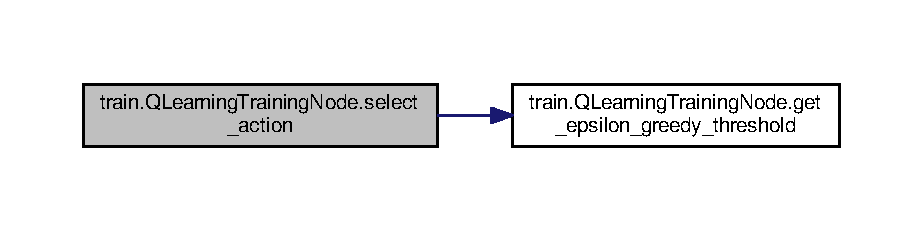
\includegraphics[width=350pt]{classtrain_1_1_q_learning_training_node_ac03f4ced7d65ef3c2cf36978796fcfda_cgraph}
\end{center}
\end{figure}




Here is the caller graph for this function\+:
\nopagebreak
\begin{figure}[H]
\begin{center}
\leavevmode
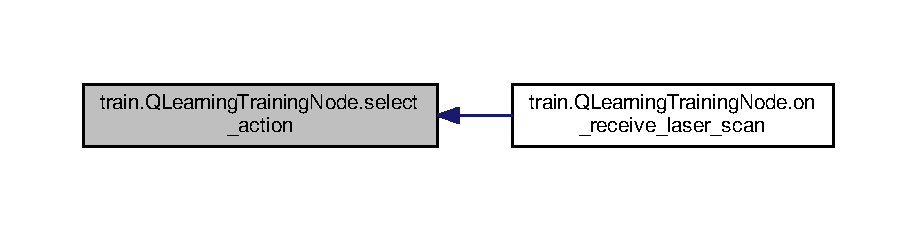
\includegraphics[width=350pt]{classtrain_1_1_q_learning_training_node_ac03f4ced7d65ef3c2cf36978796fcfda_icgraph}
\end{center}
\end{figure}




\subsection{Member Data Documentation}
\index{train\+::\+Q\+Learning\+Training\+Node@{train\+::\+Q\+Learning\+Training\+Node}!action@{action}}
\index{action@{action}!train\+::\+Q\+Learning\+Training\+Node@{train\+::\+Q\+Learning\+Training\+Node}}
\subsubsection[{\texorpdfstring{action}{action}}]{\setlength{\rightskip}{0pt plus 5cm}train.\+Q\+Learning\+Training\+Node.\+action}\hypertarget{classtrain_1_1_q_learning_training_node_ad42c35a16230d89d787b5a3a74808edf}{}\label{classtrain_1_1_q_learning_training_node_ad42c35a16230d89d787b5a3a74808edf}


Definition at line 42 of file train.\+py.

\index{train\+::\+Q\+Learning\+Training\+Node@{train\+::\+Q\+Learning\+Training\+Node}!car\+\_\+orientation@{car\+\_\+orientation}}
\index{car\+\_\+orientation@{car\+\_\+orientation}!train\+::\+Q\+Learning\+Training\+Node@{train\+::\+Q\+Learning\+Training\+Node}}
\subsubsection[{\texorpdfstring{car\+\_\+orientation}{car_orientation}}]{\setlength{\rightskip}{0pt plus 5cm}train.\+Q\+Learning\+Training\+Node.\+car\+\_\+orientation}\hypertarget{classtrain_1_1_q_learning_training_node_a016d2adc85428e64903703974f8cd79c}{}\label{classtrain_1_1_q_learning_training_node_a016d2adc85428e64903703974f8cd79c}


Definition at line 44 of file train.\+py.

\index{train\+::\+Q\+Learning\+Training\+Node@{train\+::\+Q\+Learning\+Training\+Node}!car\+\_\+position@{car\+\_\+position}}
\index{car\+\_\+position@{car\+\_\+position}!train\+::\+Q\+Learning\+Training\+Node@{train\+::\+Q\+Learning\+Training\+Node}}
\subsubsection[{\texorpdfstring{car\+\_\+position}{car_position}}]{\setlength{\rightskip}{0pt plus 5cm}train.\+Q\+Learning\+Training\+Node.\+car\+\_\+position}\hypertarget{classtrain_1_1_q_learning_training_node_ac802eca257307ce6c83897c612aa5f90}{}\label{classtrain_1_1_q_learning_training_node_ac802eca257307ce6c83897c612aa5f90}


Definition at line 43 of file train.\+py.

\index{train\+::\+Q\+Learning\+Training\+Node@{train\+::\+Q\+Learning\+Training\+Node}!cumulative\+\_\+reward@{cumulative\+\_\+reward}}
\index{cumulative\+\_\+reward@{cumulative\+\_\+reward}!train\+::\+Q\+Learning\+Training\+Node@{train\+::\+Q\+Learning\+Training\+Node}}
\subsubsection[{\texorpdfstring{cumulative\+\_\+reward}{cumulative_reward}}]{\setlength{\rightskip}{0pt plus 5cm}train.\+Q\+Learning\+Training\+Node.\+cumulative\+\_\+reward}\hypertarget{classtrain_1_1_q_learning_training_node_a4c632e44085797e564501bba836b7359}{}\label{classtrain_1_1_q_learning_training_node_a4c632e44085797e564501bba836b7359}


Definition at line 34 of file train.\+py.

\index{train\+::\+Q\+Learning\+Training\+Node@{train\+::\+Q\+Learning\+Training\+Node}!cumulative\+\_\+reward\+\_\+history@{cumulative\+\_\+reward\+\_\+history}}
\index{cumulative\+\_\+reward\+\_\+history@{cumulative\+\_\+reward\+\_\+history}!train\+::\+Q\+Learning\+Training\+Node@{train\+::\+Q\+Learning\+Training\+Node}}
\subsubsection[{\texorpdfstring{cumulative\+\_\+reward\+\_\+history}{cumulative_reward_history}}]{\setlength{\rightskip}{0pt plus 5cm}train.\+Q\+Learning\+Training\+Node.\+cumulative\+\_\+reward\+\_\+history}\hypertarget{classtrain_1_1_q_learning_training_node_aa25b9712eebb6aed6befa421814472b4}{}\label{classtrain_1_1_q_learning_training_node_aa25b9712eebb6aed6befa421814472b4}


Definition at line 39 of file train.\+py.

\index{train\+::\+Q\+Learning\+Training\+Node@{train\+::\+Q\+Learning\+Training\+Node}!drive\+\_\+forward@{drive\+\_\+forward}}
\index{drive\+\_\+forward@{drive\+\_\+forward}!train\+::\+Q\+Learning\+Training\+Node@{train\+::\+Q\+Learning\+Training\+Node}}
\subsubsection[{\texorpdfstring{drive\+\_\+forward}{drive_forward}}]{\setlength{\rightskip}{0pt plus 5cm}train.\+Q\+Learning\+Training\+Node.\+drive\+\_\+forward}\hypertarget{classtrain_1_1_q_learning_training_node_a400f047c3086a321f255b2405f2ebe1f}{}\label{classtrain_1_1_q_learning_training_node_a400f047c3086a321f255b2405f2ebe1f}


Definition at line 46 of file train.\+py.

\index{train\+::\+Q\+Learning\+Training\+Node@{train\+::\+Q\+Learning\+Training\+Node}!episode\+\_\+count@{episode\+\_\+count}}
\index{episode\+\_\+count@{episode\+\_\+count}!train\+::\+Q\+Learning\+Training\+Node@{train\+::\+Q\+Learning\+Training\+Node}}
\subsubsection[{\texorpdfstring{episode\+\_\+count}{episode_count}}]{\setlength{\rightskip}{0pt plus 5cm}train.\+Q\+Learning\+Training\+Node.\+episode\+\_\+count}\hypertarget{classtrain_1_1_q_learning_training_node_a5bef341c2aa0b019a190efb961701cdc}{}\label{classtrain_1_1_q_learning_training_node_a5bef341c2aa0b019a190efb961701cdc}


Definition at line 30 of file train.\+py.

\index{train\+::\+Q\+Learning\+Training\+Node@{train\+::\+Q\+Learning\+Training\+Node}!episode\+\_\+length@{episode\+\_\+length}}
\index{episode\+\_\+length@{episode\+\_\+length}!train\+::\+Q\+Learning\+Training\+Node@{train\+::\+Q\+Learning\+Training\+Node}}
\subsubsection[{\texorpdfstring{episode\+\_\+length}{episode_length}}]{\setlength{\rightskip}{0pt plus 5cm}train.\+Q\+Learning\+Training\+Node.\+episode\+\_\+length}\hypertarget{classtrain_1_1_q_learning_training_node_abaa1cd9793d6724977d7b9451e36bc3b}{}\label{classtrain_1_1_q_learning_training_node_abaa1cd9793d6724977d7b9451e36bc3b}


Definition at line 31 of file train.\+py.

\index{train\+::\+Q\+Learning\+Training\+Node@{train\+::\+Q\+Learning\+Training\+Node}!episode\+\_\+length\+\_\+history@{episode\+\_\+length\+\_\+history}}
\index{episode\+\_\+length\+\_\+history@{episode\+\_\+length\+\_\+history}!train\+::\+Q\+Learning\+Training\+Node@{train\+::\+Q\+Learning\+Training\+Node}}
\subsubsection[{\texorpdfstring{episode\+\_\+length\+\_\+history}{episode_length_history}}]{\setlength{\rightskip}{0pt plus 5cm}train.\+Q\+Learning\+Training\+Node.\+episode\+\_\+length\+\_\+history}\hypertarget{classtrain_1_1_q_learning_training_node_af81cfd1d0306828d0ff901faf85df6b3}{}\label{classtrain_1_1_q_learning_training_node_af81cfd1d0306828d0ff901faf85df6b3}


Definition at line 38 of file train.\+py.

\index{train\+::\+Q\+Learning\+Training\+Node@{train\+::\+Q\+Learning\+Training\+Node}!episode\+\_\+result\+\_\+publisher@{episode\+\_\+result\+\_\+publisher}}
\index{episode\+\_\+result\+\_\+publisher@{episode\+\_\+result\+\_\+publisher}!train\+::\+Q\+Learning\+Training\+Node@{train\+::\+Q\+Learning\+Training\+Node}}
\subsubsection[{\texorpdfstring{episode\+\_\+result\+\_\+publisher}{episode_result_publisher}}]{\setlength{\rightskip}{0pt plus 5cm}train.\+Q\+Learning\+Training\+Node.\+episode\+\_\+result\+\_\+publisher}\hypertarget{classtrain_1_1_q_learning_training_node_a7fef779ba6b1592b9ed2837abe5ae6ae}{}\label{classtrain_1_1_q_learning_training_node_a7fef779ba6b1592b9ed2837abe5ae6ae}


Definition at line 63 of file train.\+py.

\index{train\+::\+Q\+Learning\+Training\+Node@{train\+::\+Q\+Learning\+Training\+Node}!episode\+\_\+start\+\_\+time\+\_\+real@{episode\+\_\+start\+\_\+time\+\_\+real}}
\index{episode\+\_\+start\+\_\+time\+\_\+real@{episode\+\_\+start\+\_\+time\+\_\+real}!train\+::\+Q\+Learning\+Training\+Node@{train\+::\+Q\+Learning\+Training\+Node}}
\subsubsection[{\texorpdfstring{episode\+\_\+start\+\_\+time\+\_\+real}{episode_start_time_real}}]{\setlength{\rightskip}{0pt plus 5cm}train.\+Q\+Learning\+Training\+Node.\+episode\+\_\+start\+\_\+time\+\_\+real}\hypertarget{classtrain_1_1_q_learning_training_node_a8efbf39c7dcf595fb7c02121c66f9f53}{}\label{classtrain_1_1_q_learning_training_node_a8efbf39c7dcf595fb7c02121c66f9f53}


Definition at line 50 of file train.\+py.

\index{train\+::\+Q\+Learning\+Training\+Node@{train\+::\+Q\+Learning\+Training\+Node}!episode\+\_\+start\+\_\+time\+\_\+sim@{episode\+\_\+start\+\_\+time\+\_\+sim}}
\index{episode\+\_\+start\+\_\+time\+\_\+sim@{episode\+\_\+start\+\_\+time\+\_\+sim}!train\+::\+Q\+Learning\+Training\+Node@{train\+::\+Q\+Learning\+Training\+Node}}
\subsubsection[{\texorpdfstring{episode\+\_\+start\+\_\+time\+\_\+sim}{episode_start_time_sim}}]{\setlength{\rightskip}{0pt plus 5cm}train.\+Q\+Learning\+Training\+Node.\+episode\+\_\+start\+\_\+time\+\_\+sim}\hypertarget{classtrain_1_1_q_learning_training_node_aaba249fe751adb0b4167b350ee2ea7a1}{}\label{classtrain_1_1_q_learning_training_node_aaba249fe751adb0b4167b350ee2ea7a1}


Definition at line 51 of file train.\+py.

\index{train\+::\+Q\+Learning\+Training\+Node@{train\+::\+Q\+Learning\+Training\+Node}!is\+\_\+terminal\+\_\+step@{is\+\_\+terminal\+\_\+step}}
\index{is\+\_\+terminal\+\_\+step@{is\+\_\+terminal\+\_\+step}!train\+::\+Q\+Learning\+Training\+Node@{train\+::\+Q\+Learning\+Training\+Node}}
\subsubsection[{\texorpdfstring{is\+\_\+terminal\+\_\+step}{is_terminal_step}}]{\setlength{\rightskip}{0pt plus 5cm}train.\+Q\+Learning\+Training\+Node.\+is\+\_\+terminal\+\_\+step}\hypertarget{classtrain_1_1_q_learning_training_node_a0f8d5e71ae52a959d5248f57ac55829a}{}\label{classtrain_1_1_q_learning_training_node_a0f8d5e71ae52a959d5248f57ac55829a}


Definition at line 35 of file train.\+py.

\index{train\+::\+Q\+Learning\+Training\+Node@{train\+::\+Q\+Learning\+Training\+Node}!memory@{memory}}
\index{memory@{memory}!train\+::\+Q\+Learning\+Training\+Node@{train\+::\+Q\+Learning\+Training\+Node}}
\subsubsection[{\texorpdfstring{memory}{memory}}]{\setlength{\rightskip}{0pt plus 5cm}train.\+Q\+Learning\+Training\+Node.\+memory}\hypertarget{classtrain_1_1_q_learning_training_node_a49440485cce2f2f3fe9575456a562098}{}\label{classtrain_1_1_q_learning_training_node_a49440485cce2f2f3fe9575456a562098}


Definition at line 57 of file train.\+py.

\index{train\+::\+Q\+Learning\+Training\+Node@{train\+::\+Q\+Learning\+Training\+Node}!net\+\_\+output\+\_\+debug\+\_\+string@{net\+\_\+output\+\_\+debug\+\_\+string}}
\index{net\+\_\+output\+\_\+debug\+\_\+string@{net\+\_\+output\+\_\+debug\+\_\+string}!train\+::\+Q\+Learning\+Training\+Node@{train\+::\+Q\+Learning\+Training\+Node}}
\subsubsection[{\texorpdfstring{net\+\_\+output\+\_\+debug\+\_\+string}{net_output_debug_string}}]{\setlength{\rightskip}{0pt plus 5cm}train.\+Q\+Learning\+Training\+Node.\+net\+\_\+output\+\_\+debug\+\_\+string}\hypertarget{classtrain_1_1_q_learning_training_node_a5837c478232e1d4cc646bfbadbdd2ff2}{}\label{classtrain_1_1_q_learning_training_node_a5837c478232e1d4cc646bfbadbdd2ff2}


Definition at line 37 of file train.\+py.

\index{train\+::\+Q\+Learning\+Training\+Node@{train\+::\+Q\+Learning\+Training\+Node}!optimization\+\_\+step\+\_\+count@{optimization\+\_\+step\+\_\+count}}
\index{optimization\+\_\+step\+\_\+count@{optimization\+\_\+step\+\_\+count}!train\+::\+Q\+Learning\+Training\+Node@{train\+::\+Q\+Learning\+Training\+Node}}
\subsubsection[{\texorpdfstring{optimization\+\_\+step\+\_\+count}{optimization_step_count}}]{\setlength{\rightskip}{0pt plus 5cm}train.\+Q\+Learning\+Training\+Node.\+optimization\+\_\+step\+\_\+count}\hypertarget{classtrain_1_1_q_learning_training_node_a876c1cedd4eabcca4e9a0ee6e0922752}{}\label{classtrain_1_1_q_learning_training_node_a876c1cedd4eabcca4e9a0ee6e0922752}


Definition at line 33 of file train.\+py.

\index{train\+::\+Q\+Learning\+Training\+Node@{train\+::\+Q\+Learning\+Training\+Node}!optimizer@{optimizer}}
\index{optimizer@{optimizer}!train\+::\+Q\+Learning\+Training\+Node@{train\+::\+Q\+Learning\+Training\+Node}}
\subsubsection[{\texorpdfstring{optimizer}{optimizer}}]{\setlength{\rightskip}{0pt plus 5cm}train.\+Q\+Learning\+Training\+Node.\+optimizer}\hypertarget{classtrain_1_1_q_learning_training_node_a2cd6ba599812ec0edffba7869f4f27d9}{}\label{classtrain_1_1_q_learning_training_node_a2cd6ba599812ec0edffba7869f4f27d9}


Definition at line 56 of file train.\+py.

\index{train\+::\+Q\+Learning\+Training\+Node@{train\+::\+Q\+Learning\+Training\+Node}!real\+\_\+time\+\_\+factor@{real\+\_\+time\+\_\+factor}}
\index{real\+\_\+time\+\_\+factor@{real\+\_\+time\+\_\+factor}!train\+::\+Q\+Learning\+Training\+Node@{train\+::\+Q\+Learning\+Training\+Node}}
\subsubsection[{\texorpdfstring{real\+\_\+time\+\_\+factor}{real_time_factor}}]{\setlength{\rightskip}{0pt plus 5cm}train.\+Q\+Learning\+Training\+Node.\+real\+\_\+time\+\_\+factor}\hypertarget{classtrain_1_1_q_learning_training_node_a407532bec47855fec93201fa87fe80ab}{}\label{classtrain_1_1_q_learning_training_node_a407532bec47855fec93201fa87fe80ab}


Definition at line 49 of file train.\+py.

\index{train\+::\+Q\+Learning\+Training\+Node@{train\+::\+Q\+Learning\+Training\+Node}!state@{state}}
\index{state@{state}!train\+::\+Q\+Learning\+Training\+Node@{train\+::\+Q\+Learning\+Training\+Node}}
\subsubsection[{\texorpdfstring{state}{state}}]{\setlength{\rightskip}{0pt plus 5cm}train.\+Q\+Learning\+Training\+Node.\+state}\hypertarget{classtrain_1_1_q_learning_training_node_a6e860eb510dc030f536d26c2a3fcc33c}{}\label{classtrain_1_1_q_learning_training_node_a6e860eb510dc030f536d26c2a3fcc33c}


Definition at line 41 of file train.\+py.

\index{train\+::\+Q\+Learning\+Training\+Node@{train\+::\+Q\+Learning\+Training\+Node}!steps\+\_\+with\+\_\+wrong\+\_\+orientation@{steps\+\_\+with\+\_\+wrong\+\_\+orientation}}
\index{steps\+\_\+with\+\_\+wrong\+\_\+orientation@{steps\+\_\+with\+\_\+wrong\+\_\+orientation}!train\+::\+Q\+Learning\+Training\+Node@{train\+::\+Q\+Learning\+Training\+Node}}
\subsubsection[{\texorpdfstring{steps\+\_\+with\+\_\+wrong\+\_\+orientation}{steps_with_wrong_orientation}}]{\setlength{\rightskip}{0pt plus 5cm}train.\+Q\+Learning\+Training\+Node.\+steps\+\_\+with\+\_\+wrong\+\_\+orientation}\hypertarget{classtrain_1_1_q_learning_training_node_a87a28e543665823ac18758f6a4460d7a}{}\label{classtrain_1_1_q_learning_training_node_a87a28e543665823ac18758f6a4460d7a}


Definition at line 47 of file train.\+py.

\index{train\+::\+Q\+Learning\+Training\+Node@{train\+::\+Q\+Learning\+Training\+Node}!total\+\_\+step\+\_\+count@{total\+\_\+step\+\_\+count}}
\index{total\+\_\+step\+\_\+count@{total\+\_\+step\+\_\+count}!train\+::\+Q\+Learning\+Training\+Node@{train\+::\+Q\+Learning\+Training\+Node}}
\subsubsection[{\texorpdfstring{total\+\_\+step\+\_\+count}{total_step_count}}]{\setlength{\rightskip}{0pt plus 5cm}train.\+Q\+Learning\+Training\+Node.\+total\+\_\+step\+\_\+count}\hypertarget{classtrain_1_1_q_learning_training_node_aa583fe782e5ae47cc64dd44b92fd2e71}{}\label{classtrain_1_1_q_learning_training_node_aa583fe782e5ae47cc64dd44b92fd2e71}


Definition at line 32 of file train.\+py.



The documentation for this class was generated from the following file\+:\begin{DoxyCompactItemize}
\item 
/home/travis/build/\+Autonomous-\/\+Racing-\/\+P\+G/ros.\+package/docs/master/ros\+\_\+ws/src/autonomous/q\+\_\+learning/scripts/\hyperlink{q__learning_2scripts_2train_8py}{train.\+py}\end{DoxyCompactItemize}

\hypertarget{class_rviz_geometry_publisher}{}\section{Rviz\+Geometry\+Publisher Class Reference}
\label{class_rviz_geometry_publisher}\index{Rviz\+Geometry\+Publisher@{Rviz\+Geometry\+Publisher}}


{\ttfamily \#include $<$rviz\+\_\+geometry\+\_\+publisher.\+h$>$}

\subsection*{Public Member Functions}
\begin{DoxyCompactItemize}
\item 
\hyperlink{class_rviz_geometry_publisher_ace4d6e2e5dd88168dd4e6c5f528a255e}{Rviz\+Geometry\+Publisher} (ros\+::\+Node\+Handle node\+\_\+handle, const std\+::string \&topic, const std\+::string \&frame)
\item 
void \hyperlink{class_rviz_geometry_publisher_a4448e349606332f087c4deda0a710032}{draw\+Line} (int id, geometry\+\_\+msgs\+::\+Point point1, geometry\+\_\+msgs\+::\+Point point2, std\+\_\+msgs\+::\+Color\+R\+G\+BA color, float width)
\item 
\hyperlink{class_rviz_geometry_publisher_ace4d6e2e5dd88168dd4e6c5f528a255e}{Rviz\+Geometry\+Publisher} (ros\+::\+Node\+Handle node\+\_\+handle, const std\+::string \&topic, const std\+::string \&frame)
\item 
void \hyperlink{class_rviz_geometry_publisher_a4448e349606332f087c4deda0a710032}{draw\+Line} (int id, geometry\+\_\+msgs\+::\+Point point1, geometry\+\_\+msgs\+::\+Point point2, std\+\_\+msgs\+::\+Color\+R\+G\+BA color, float width)
\end{DoxyCompactItemize}


\subsection{Detailed Description}


Definition at line 10 of file rviz\+\_\+geometry\+\_\+publisher.\+h.



\subsection{Constructor \& Destructor Documentation}
\index{Rviz\+Geometry\+Publisher@{Rviz\+Geometry\+Publisher}!Rviz\+Geometry\+Publisher@{Rviz\+Geometry\+Publisher}}
\index{Rviz\+Geometry\+Publisher@{Rviz\+Geometry\+Publisher}!Rviz\+Geometry\+Publisher@{Rviz\+Geometry\+Publisher}}
\subsubsection[{\texorpdfstring{Rviz\+Geometry\+Publisher(ros\+::\+Node\+Handle node\+\_\+handle, const std\+::string \&topic, const std\+::string \&frame)}{RvizGeometryPublisher(ros::NodeHandle node_handle, const std::string &topic, const std::string &frame)}}]{\setlength{\rightskip}{0pt plus 5cm}Rviz\+Geometry\+Publisher\+::\+Rviz\+Geometry\+Publisher (
\begin{DoxyParamCaption}
\item[{ros\+::\+Node\+Handle}]{node\+\_\+handle, }
\item[{const std\+::string \&}]{topic, }
\item[{const std\+::string \&}]{frame}
\end{DoxyParamCaption}
)}\hypertarget{class_rviz_geometry_publisher_ace4d6e2e5dd88168dd4e6c5f528a255e}{}\label{class_rviz_geometry_publisher_ace4d6e2e5dd88168dd4e6c5f528a255e}


Definition at line 3 of file rviz\+\_\+geometry\+\_\+publisher.\+cpp.

\index{Rviz\+Geometry\+Publisher@{Rviz\+Geometry\+Publisher}!Rviz\+Geometry\+Publisher@{Rviz\+Geometry\+Publisher}}
\index{Rviz\+Geometry\+Publisher@{Rviz\+Geometry\+Publisher}!Rviz\+Geometry\+Publisher@{Rviz\+Geometry\+Publisher}}
\subsubsection[{\texorpdfstring{Rviz\+Geometry\+Publisher(ros\+::\+Node\+Handle node\+\_\+handle, const std\+::string \&topic, const std\+::string \&frame)}{RvizGeometryPublisher(ros::NodeHandle node_handle, const std::string &topic, const std::string &frame)}}]{\setlength{\rightskip}{0pt plus 5cm}Rviz\+Geometry\+Publisher\+::\+Rviz\+Geometry\+Publisher (
\begin{DoxyParamCaption}
\item[{ros\+::\+Node\+Handle}]{node\+\_\+handle, }
\item[{const std\+::string \&}]{topic, }
\item[{const std\+::string \&}]{frame}
\end{DoxyParamCaption}
)}\hypertarget{class_rviz_geometry_publisher_ace4d6e2e5dd88168dd4e6c5f528a255e}{}\label{class_rviz_geometry_publisher_ace4d6e2e5dd88168dd4e6c5f528a255e}


\subsection{Member Function Documentation}
\index{Rviz\+Geometry\+Publisher@{Rviz\+Geometry\+Publisher}!draw\+Line@{draw\+Line}}
\index{draw\+Line@{draw\+Line}!Rviz\+Geometry\+Publisher@{Rviz\+Geometry\+Publisher}}
\subsubsection[{\texorpdfstring{draw\+Line(int id, geometry\+\_\+msgs\+::\+Point point1, geometry\+\_\+msgs\+::\+Point point2, std\+\_\+msgs\+::\+Color\+R\+G\+B\+A color, float width)}{drawLine(int id, geometry_msgs::Point point1, geometry_msgs::Point point2, std_msgs::ColorRGBA color, float width)}}]{\setlength{\rightskip}{0pt plus 5cm}void Rviz\+Geometry\+Publisher\+::draw\+Line (
\begin{DoxyParamCaption}
\item[{int}]{id, }
\item[{geometry\+\_\+msgs\+::\+Point}]{point1, }
\item[{geometry\+\_\+msgs\+::\+Point}]{point2, }
\item[{std\+\_\+msgs\+::\+Color\+R\+G\+BA}]{color, }
\item[{float}]{width}
\end{DoxyParamCaption}
)}\hypertarget{class_rviz_geometry_publisher_a4448e349606332f087c4deda0a710032}{}\label{class_rviz_geometry_publisher_a4448e349606332f087c4deda0a710032}


Definition at line 10 of file rviz\+\_\+geometry\+\_\+publisher.\+cpp.



Here is the caller graph for this function\+:
\nopagebreak
\begin{figure}[H]
\begin{center}
\leavevmode
\includegraphics[width=350pt]{class_rviz_geometry_publisher_a4448e349606332f087c4deda0a710032_icgraph}
\end{center}
\end{figure}


\index{Rviz\+Geometry\+Publisher@{Rviz\+Geometry\+Publisher}!draw\+Line@{draw\+Line}}
\index{draw\+Line@{draw\+Line}!Rviz\+Geometry\+Publisher@{Rviz\+Geometry\+Publisher}}
\subsubsection[{\texorpdfstring{draw\+Line(int id, geometry\+\_\+msgs\+::\+Point point1, geometry\+\_\+msgs\+::\+Point point2, std\+\_\+msgs\+::\+Color\+R\+G\+B\+A color, float width)}{drawLine(int id, geometry_msgs::Point point1, geometry_msgs::Point point2, std_msgs::ColorRGBA color, float width)}}]{\setlength{\rightskip}{0pt plus 5cm}void Rviz\+Geometry\+Publisher\+::draw\+Line (
\begin{DoxyParamCaption}
\item[{int}]{id, }
\item[{geometry\+\_\+msgs\+::\+Point}]{point1, }
\item[{geometry\+\_\+msgs\+::\+Point}]{point2, }
\item[{std\+\_\+msgs\+::\+Color\+R\+G\+BA}]{color, }
\item[{float}]{width}
\end{DoxyParamCaption}
)}\hypertarget{class_rviz_geometry_publisher_a4448e349606332f087c4deda0a710032}{}\label{class_rviz_geometry_publisher_a4448e349606332f087c4deda0a710032}


The documentation for this class was generated from the following files\+:\begin{DoxyCompactItemize}
\item 
/home/travis/build/\+Autonomous-\/\+Racing-\/\+P\+G/ros.\+package/docs/master/ros\+\_\+ws/src/autonomous/emergency\+\_\+stop/include/\hyperlink{emergency__stop_2include_2rviz__geometry__publisher_8h}{rviz\+\_\+geometry\+\_\+publisher.\+h}\item 
/home/travis/build/\+Autonomous-\/\+Racing-\/\+P\+G/ros.\+package/docs/master/ros\+\_\+ws/src/autonomous/emergency\+\_\+stop/src/\hyperlink{emergency__stop_2src_2rviz__geometry__publisher_8cpp}{rviz\+\_\+geometry\+\_\+publisher.\+cpp}\end{DoxyCompactItemize}

\hypertarget{classsimulation__tools_1_1lap__timer_1_1_timer}{}\section{simulation\+\_\+tools.\+lap\+\_\+timer.\+Timer Class Reference}
\label{classsimulation__tools_1_1lap__timer_1_1_timer}\index{simulation\+\_\+tools.\+lap\+\_\+timer.\+Timer@{simulation\+\_\+tools.\+lap\+\_\+timer.\+Timer}}
\subsection*{Public Member Functions}
\begin{DoxyCompactItemize}
\item 
def \hyperlink{classsimulation__tools_1_1lap__timer_1_1_timer_a526781ad4e5c09fbe04dda1e5a3f3fd9}{\+\_\+\+\_\+init\+\_\+\+\_\+} (self, \hyperlink{classsimulation__tools_1_1lap__timer_1_1_timer_a9bf911e55976cb1d04b10440cea407c1}{name}, \hyperlink{classsimulation__tools_1_1lap__timer_1_1_timer_ae042ce601347d175584be16d8166a74e}{checkpoints})
\item 
def \hyperlink{classsimulation__tools_1_1lap__timer_1_1_timer_ae9b21a99e315e66e34311c6b9feeb0e8}{update} (self, position)
\item 
def \hyperlink{classsimulation__tools_1_1lap__timer_1_1_timer_a9fac2e869ccbcd86651e333301d8cc33}{complete\+\_\+lap} (self)
\end{DoxyCompactItemize}
\subsection*{Public Attributes}
\begin{DoxyCompactItemize}
\item 
\hyperlink{classsimulation__tools_1_1lap__timer_1_1_timer_a9bf911e55976cb1d04b10440cea407c1}{name}
\item 
\hyperlink{classsimulation__tools_1_1lap__timer_1_1_timer_ae042ce601347d175584be16d8166a74e}{checkpoints}
\item 
\hyperlink{classsimulation__tools_1_1lap__timer_1_1_timer_a74b19b620b1f59ce1d558524c275f4c3}{next\+\_\+checkpoint}
\item 
\hyperlink{classsimulation__tools_1_1lap__timer_1_1_timer_a5f5e50dc374ab88c05748ab49392b881}{history}
\item 
\hyperlink{classsimulation__tools_1_1lap__timer_1_1_timer_afc51d0e4a6aa0e19be5c8622352b9afe}{start}
\end{DoxyCompactItemize}


\subsection{Detailed Description}


Definition at line 30 of file lap\+\_\+timer.\+py.



\subsection{Constructor \& Destructor Documentation}
\index{simulation\+\_\+tools\+::lap\+\_\+timer\+::\+Timer@{simulation\+\_\+tools\+::lap\+\_\+timer\+::\+Timer}!\+\_\+\+\_\+init\+\_\+\+\_\+@{\+\_\+\+\_\+init\+\_\+\+\_\+}}
\index{\+\_\+\+\_\+init\+\_\+\+\_\+@{\+\_\+\+\_\+init\+\_\+\+\_\+}!simulation\+\_\+tools\+::lap\+\_\+timer\+::\+Timer@{simulation\+\_\+tools\+::lap\+\_\+timer\+::\+Timer}}
\subsubsection[{\texorpdfstring{\+\_\+\+\_\+init\+\_\+\+\_\+(self, name, checkpoints)}{__init__(self, name, checkpoints)}}]{\setlength{\rightskip}{0pt plus 5cm}def simulation\+\_\+tools.\+lap\+\_\+timer.\+Timer.\+\_\+\+\_\+init\+\_\+\+\_\+ (
\begin{DoxyParamCaption}
\item[{}]{self, }
\item[{}]{name, }
\item[{}]{checkpoints}
\end{DoxyParamCaption}
)}\hypertarget{classsimulation__tools_1_1lap__timer_1_1_timer_a526781ad4e5c09fbe04dda1e5a3f3fd9}{}\label{classsimulation__tools_1_1lap__timer_1_1_timer_a526781ad4e5c09fbe04dda1e5a3f3fd9}


Definition at line 31 of file lap\+\_\+timer.\+py.



\subsection{Member Function Documentation}
\index{simulation\+\_\+tools\+::lap\+\_\+timer\+::\+Timer@{simulation\+\_\+tools\+::lap\+\_\+timer\+::\+Timer}!complete\+\_\+lap@{complete\+\_\+lap}}
\index{complete\+\_\+lap@{complete\+\_\+lap}!simulation\+\_\+tools\+::lap\+\_\+timer\+::\+Timer@{simulation\+\_\+tools\+::lap\+\_\+timer\+::\+Timer}}
\subsubsection[{\texorpdfstring{complete\+\_\+lap(self)}{complete_lap(self)}}]{\setlength{\rightskip}{0pt plus 5cm}def simulation\+\_\+tools.\+lap\+\_\+timer.\+Timer.\+complete\+\_\+lap (
\begin{DoxyParamCaption}
\item[{}]{self}
\end{DoxyParamCaption}
)}\hypertarget{classsimulation__tools_1_1lap__timer_1_1_timer_a9fac2e869ccbcd86651e333301d8cc33}{}\label{classsimulation__tools_1_1lap__timer_1_1_timer_a9fac2e869ccbcd86651e333301d8cc33}


Definition at line 52 of file lap\+\_\+timer.\+py.



Here is the call graph for this function\+:
\nopagebreak
\begin{figure}[H]
\begin{center}
\leavevmode
\includegraphics[width=350pt]{classsimulation__tools_1_1lap__timer_1_1_timer_a9fac2e869ccbcd86651e333301d8cc33_cgraph}
\end{center}
\end{figure}




Here is the caller graph for this function\+:
\nopagebreak
\begin{figure}[H]
\begin{center}
\leavevmode
\includegraphics[width=350pt]{classsimulation__tools_1_1lap__timer_1_1_timer_a9fac2e869ccbcd86651e333301d8cc33_icgraph}
\end{center}
\end{figure}


\index{simulation\+\_\+tools\+::lap\+\_\+timer\+::\+Timer@{simulation\+\_\+tools\+::lap\+\_\+timer\+::\+Timer}!update@{update}}
\index{update@{update}!simulation\+\_\+tools\+::lap\+\_\+timer\+::\+Timer@{simulation\+\_\+tools\+::lap\+\_\+timer\+::\+Timer}}
\subsubsection[{\texorpdfstring{update(self, position)}{update(self, position)}}]{\setlength{\rightskip}{0pt plus 5cm}def simulation\+\_\+tools.\+lap\+\_\+timer.\+Timer.\+update (
\begin{DoxyParamCaption}
\item[{}]{self, }
\item[{}]{position}
\end{DoxyParamCaption}
)}\hypertarget{classsimulation__tools_1_1lap__timer_1_1_timer_ae9b21a99e315e66e34311c6b9feeb0e8}{}\label{classsimulation__tools_1_1lap__timer_1_1_timer_ae9b21a99e315e66e34311c6b9feeb0e8}


Definition at line 38 of file lap\+\_\+timer.\+py.



Here is the call graph for this function\+:
\nopagebreak
\begin{figure}[H]
\begin{center}
\leavevmode
\includegraphics[width=350pt]{classsimulation__tools_1_1lap__timer_1_1_timer_ae9b21a99e315e66e34311c6b9feeb0e8_cgraph}
\end{center}
\end{figure}




\subsection{Member Data Documentation}
\index{simulation\+\_\+tools\+::lap\+\_\+timer\+::\+Timer@{simulation\+\_\+tools\+::lap\+\_\+timer\+::\+Timer}!checkpoints@{checkpoints}}
\index{checkpoints@{checkpoints}!simulation\+\_\+tools\+::lap\+\_\+timer\+::\+Timer@{simulation\+\_\+tools\+::lap\+\_\+timer\+::\+Timer}}
\subsubsection[{\texorpdfstring{checkpoints}{checkpoints}}]{\setlength{\rightskip}{0pt plus 5cm}simulation\+\_\+tools.\+lap\+\_\+timer.\+Timer.\+checkpoints}\hypertarget{classsimulation__tools_1_1lap__timer_1_1_timer_ae042ce601347d175584be16d8166a74e}{}\label{classsimulation__tools_1_1lap__timer_1_1_timer_ae042ce601347d175584be16d8166a74e}


Definition at line 33 of file lap\+\_\+timer.\+py.

\index{simulation\+\_\+tools\+::lap\+\_\+timer\+::\+Timer@{simulation\+\_\+tools\+::lap\+\_\+timer\+::\+Timer}!history@{history}}
\index{history@{history}!simulation\+\_\+tools\+::lap\+\_\+timer\+::\+Timer@{simulation\+\_\+tools\+::lap\+\_\+timer\+::\+Timer}}
\subsubsection[{\texorpdfstring{history}{history}}]{\setlength{\rightskip}{0pt plus 5cm}simulation\+\_\+tools.\+lap\+\_\+timer.\+Timer.\+history}\hypertarget{classsimulation__tools_1_1lap__timer_1_1_timer_a5f5e50dc374ab88c05748ab49392b881}{}\label{classsimulation__tools_1_1lap__timer_1_1_timer_a5f5e50dc374ab88c05748ab49392b881}


Definition at line 35 of file lap\+\_\+timer.\+py.

\index{simulation\+\_\+tools\+::lap\+\_\+timer\+::\+Timer@{simulation\+\_\+tools\+::lap\+\_\+timer\+::\+Timer}!name@{name}}
\index{name@{name}!simulation\+\_\+tools\+::lap\+\_\+timer\+::\+Timer@{simulation\+\_\+tools\+::lap\+\_\+timer\+::\+Timer}}
\subsubsection[{\texorpdfstring{name}{name}}]{\setlength{\rightskip}{0pt plus 5cm}simulation\+\_\+tools.\+lap\+\_\+timer.\+Timer.\+name}\hypertarget{classsimulation__tools_1_1lap__timer_1_1_timer_a9bf911e55976cb1d04b10440cea407c1}{}\label{classsimulation__tools_1_1lap__timer_1_1_timer_a9bf911e55976cb1d04b10440cea407c1}


Definition at line 32 of file lap\+\_\+timer.\+py.

\index{simulation\+\_\+tools\+::lap\+\_\+timer\+::\+Timer@{simulation\+\_\+tools\+::lap\+\_\+timer\+::\+Timer}!next\+\_\+checkpoint@{next\+\_\+checkpoint}}
\index{next\+\_\+checkpoint@{next\+\_\+checkpoint}!simulation\+\_\+tools\+::lap\+\_\+timer\+::\+Timer@{simulation\+\_\+tools\+::lap\+\_\+timer\+::\+Timer}}
\subsubsection[{\texorpdfstring{next\+\_\+checkpoint}{next_checkpoint}}]{\setlength{\rightskip}{0pt plus 5cm}simulation\+\_\+tools.\+lap\+\_\+timer.\+Timer.\+next\+\_\+checkpoint}\hypertarget{classsimulation__tools_1_1lap__timer_1_1_timer_a74b19b620b1f59ce1d558524c275f4c3}{}\label{classsimulation__tools_1_1lap__timer_1_1_timer_a74b19b620b1f59ce1d558524c275f4c3}


Definition at line 34 of file lap\+\_\+timer.\+py.

\index{simulation\+\_\+tools\+::lap\+\_\+timer\+::\+Timer@{simulation\+\_\+tools\+::lap\+\_\+timer\+::\+Timer}!start@{start}}
\index{start@{start}!simulation\+\_\+tools\+::lap\+\_\+timer\+::\+Timer@{simulation\+\_\+tools\+::lap\+\_\+timer\+::\+Timer}}
\subsubsection[{\texorpdfstring{start}{start}}]{\setlength{\rightskip}{0pt plus 5cm}simulation\+\_\+tools.\+lap\+\_\+timer.\+Timer.\+start}\hypertarget{classsimulation__tools_1_1lap__timer_1_1_timer_afc51d0e4a6aa0e19be5c8622352b9afe}{}\label{classsimulation__tools_1_1lap__timer_1_1_timer_afc51d0e4a6aa0e19be5c8622352b9afe}


Definition at line 36 of file lap\+\_\+timer.\+py.



The documentation for this class was generated from the following file\+:\begin{DoxyCompactItemize}
\item 
/home/travis/build/\+Autonomous-\/\+Racing-\/\+P\+G/ros.\+package/docs/master/ros\+\_\+ws/src/simulation/simulation\+\_\+tools/src/simulation\+\_\+tools/\hyperlink{lap__timer_8py}{lap\+\_\+timer.\+py}\end{DoxyCompactItemize}

\hypertarget{classsimulation__tools_1_1track_1_1_track}{}\section{simulation\+\_\+tools.\+track.\+Track Class Reference}
\label{classsimulation__tools_1_1track_1_1_track}\index{simulation\+\_\+tools.\+track.\+Track@{simulation\+\_\+tools.\+track.\+Track}}
\subsection*{Public Member Functions}
\begin{DoxyCompactItemize}
\item 
def \hyperlink{classsimulation__tools_1_1track_1_1_track_a688ef860ebacddc55c143c6202a3dab5}{\+\_\+\+\_\+init\+\_\+\+\_\+} (self, \hyperlink{classsimulation__tools_1_1track_1_1_track_ac6de34747fd382897e7f790cd9faf67c}{points})
\item 
def \hyperlink{classsimulation__tools_1_1track_1_1_track_a74c6566237436692a421615bd5cf9064}{localize} (self, point)
\item 
def \hyperlink{classsimulation__tools_1_1track_1_1_track_a65ae88cad753af6ebf71ae09fd110ac8}{get\+\_\+position} (self, total\+\_\+distance, distance\+\_\+to\+\_\+center=0)
\end{DoxyCompactItemize}
\subsection*{Public Attributes}
\begin{DoxyCompactItemize}
\item 
\hyperlink{classsimulation__tools_1_1track_1_1_track_ac6de34747fd382897e7f790cd9faf67c}{points}
\item 
\hyperlink{classsimulation__tools_1_1track_1_1_track_a69be8807eecacfd98981e206ea3a003f}{size}
\item 
\hyperlink{classsimulation__tools_1_1track_1_1_track_aa74dadec286ae8ad2f3399c6fd9e9fd9}{segment\+\_\+length}
\item 
\hyperlink{classsimulation__tools_1_1track_1_1_track_a24b60622edd3b0825f31fd6426d9380b}{length}
\item 
\hyperlink{classsimulation__tools_1_1track_1_1_track_ae944fe956579cafe73bf09d3a7c072bc}{forward}
\item 
\hyperlink{classsimulation__tools_1_1track_1_1_track_a668e3804fa2720790fb57f592c73c782}{right}
\item 
\hyperlink{classsimulation__tools_1_1track_1_1_track_a4513ffc3cdb1963bce98c678b093c40b}{cumulative\+\_\+distance}
\end{DoxyCompactItemize}


\subsection{Detailed Description}


Definition at line 50 of file track.\+py.



\subsection{Constructor \& Destructor Documentation}
\index{simulation\+\_\+tools\+::track\+::\+Track@{simulation\+\_\+tools\+::track\+::\+Track}!\+\_\+\+\_\+init\+\_\+\+\_\+@{\+\_\+\+\_\+init\+\_\+\+\_\+}}
\index{\+\_\+\+\_\+init\+\_\+\+\_\+@{\+\_\+\+\_\+init\+\_\+\+\_\+}!simulation\+\_\+tools\+::track\+::\+Track@{simulation\+\_\+tools\+::track\+::\+Track}}
\subsubsection[{\texorpdfstring{\+\_\+\+\_\+init\+\_\+\+\_\+(self, points)}{__init__(self, points)}}]{\setlength{\rightskip}{0pt plus 5cm}def simulation\+\_\+tools.\+track.\+Track.\+\_\+\+\_\+init\+\_\+\+\_\+ (
\begin{DoxyParamCaption}
\item[{}]{self, }
\item[{}]{points}
\end{DoxyParamCaption}
)}\hypertarget{classsimulation__tools_1_1track_1_1_track_a688ef860ebacddc55c143c6202a3dab5}{}\label{classsimulation__tools_1_1track_1_1_track_a688ef860ebacddc55c143c6202a3dab5}


Definition at line 51 of file track.\+py.



\subsection{Member Function Documentation}
\index{simulation\+\_\+tools\+::track\+::\+Track@{simulation\+\_\+tools\+::track\+::\+Track}!get\+\_\+position@{get\+\_\+position}}
\index{get\+\_\+position@{get\+\_\+position}!simulation\+\_\+tools\+::track\+::\+Track@{simulation\+\_\+tools\+::track\+::\+Track}}
\subsubsection[{\texorpdfstring{get\+\_\+position(self, total\+\_\+distance, distance\+\_\+to\+\_\+center=0)}{get_position(self, total_distance, distance_to_center=0)}}]{\setlength{\rightskip}{0pt plus 5cm}def simulation\+\_\+tools.\+track.\+Track.\+get\+\_\+position (
\begin{DoxyParamCaption}
\item[{}]{self, }
\item[{}]{total\+\_\+distance, }
\item[{}]{distance\+\_\+to\+\_\+center = {\ttfamily 0}}
\end{DoxyParamCaption}
)}\hypertarget{classsimulation__tools_1_1track_1_1_track_a65ae88cad753af6ebf71ae09fd110ac8}{}\label{classsimulation__tools_1_1track_1_1_track_a65ae88cad753af6ebf71ae09fd110ac8}
\begin{DoxyVerb}Returns a TrackPosition object based on the on-track distance from the start
line and the distance to the center of the track. \end{DoxyVerb}
 

Definition at line 73 of file track.\+py.

\index{simulation\+\_\+tools\+::track\+::\+Track@{simulation\+\_\+tools\+::track\+::\+Track}!localize@{localize}}
\index{localize@{localize}!simulation\+\_\+tools\+::track\+::\+Track@{simulation\+\_\+tools\+::track\+::\+Track}}
\subsubsection[{\texorpdfstring{localize(self, point)}{localize(self, point)}}]{\setlength{\rightskip}{0pt plus 5cm}def simulation\+\_\+tools.\+track.\+Track.\+localize (
\begin{DoxyParamCaption}
\item[{}]{self, }
\item[{}]{point}
\end{DoxyParamCaption}
)}\hypertarget{classsimulation__tools_1_1track_1_1_track_a74c6566237436692a421615bd5cf9064}{}\label{classsimulation__tools_1_1track_1_1_track_a74c6566237436692a421615bd5cf9064}
\begin{DoxyVerb}Returns a TrackPosition object based on a position in world space. \end{DoxyVerb}
 

Definition at line 63 of file track.\+py.



\subsection{Member Data Documentation}
\index{simulation\+\_\+tools\+::track\+::\+Track@{simulation\+\_\+tools\+::track\+::\+Track}!cumulative\+\_\+distance@{cumulative\+\_\+distance}}
\index{cumulative\+\_\+distance@{cumulative\+\_\+distance}!simulation\+\_\+tools\+::track\+::\+Track@{simulation\+\_\+tools\+::track\+::\+Track}}
\subsubsection[{\texorpdfstring{cumulative\+\_\+distance}{cumulative_distance}}]{\setlength{\rightskip}{0pt plus 5cm}simulation\+\_\+tools.\+track.\+Track.\+cumulative\+\_\+distance}\hypertarget{classsimulation__tools_1_1track_1_1_track_a4513ffc3cdb1963bce98c678b093c40b}{}\label{classsimulation__tools_1_1track_1_1_track_a4513ffc3cdb1963bce98c678b093c40b}


Definition at line 60 of file track.\+py.

\index{simulation\+\_\+tools\+::track\+::\+Track@{simulation\+\_\+tools\+::track\+::\+Track}!forward@{forward}}
\index{forward@{forward}!simulation\+\_\+tools\+::track\+::\+Track@{simulation\+\_\+tools\+::track\+::\+Track}}
\subsubsection[{\texorpdfstring{forward}{forward}}]{\setlength{\rightskip}{0pt plus 5cm}simulation\+\_\+tools.\+track.\+Track.\+forward}\hypertarget{classsimulation__tools_1_1track_1_1_track_ae944fe956579cafe73bf09d3a7c072bc}{}\label{classsimulation__tools_1_1track_1_1_track_ae944fe956579cafe73bf09d3a7c072bc}


Definition at line 57 of file track.\+py.

\index{simulation\+\_\+tools\+::track\+::\+Track@{simulation\+\_\+tools\+::track\+::\+Track}!length@{length}}
\index{length@{length}!simulation\+\_\+tools\+::track\+::\+Track@{simulation\+\_\+tools\+::track\+::\+Track}}
\subsubsection[{\texorpdfstring{length}{length}}]{\setlength{\rightskip}{0pt plus 5cm}simulation\+\_\+tools.\+track.\+Track.\+length}\hypertarget{classsimulation__tools_1_1track_1_1_track_a24b60622edd3b0825f31fd6426d9380b}{}\label{classsimulation__tools_1_1track_1_1_track_a24b60622edd3b0825f31fd6426d9380b}


Definition at line 56 of file track.\+py.

\index{simulation\+\_\+tools\+::track\+::\+Track@{simulation\+\_\+tools\+::track\+::\+Track}!points@{points}}
\index{points@{points}!simulation\+\_\+tools\+::track\+::\+Track@{simulation\+\_\+tools\+::track\+::\+Track}}
\subsubsection[{\texorpdfstring{points}{points}}]{\setlength{\rightskip}{0pt plus 5cm}simulation\+\_\+tools.\+track.\+Track.\+points}\hypertarget{classsimulation__tools_1_1track_1_1_track_ac6de34747fd382897e7f790cd9faf67c}{}\label{classsimulation__tools_1_1track_1_1_track_ac6de34747fd382897e7f790cd9faf67c}


Definition at line 52 of file track.\+py.

\index{simulation\+\_\+tools\+::track\+::\+Track@{simulation\+\_\+tools\+::track\+::\+Track}!right@{right}}
\index{right@{right}!simulation\+\_\+tools\+::track\+::\+Track@{simulation\+\_\+tools\+::track\+::\+Track}}
\subsubsection[{\texorpdfstring{right}{right}}]{\setlength{\rightskip}{0pt plus 5cm}simulation\+\_\+tools.\+track.\+Track.\+right}\hypertarget{classsimulation__tools_1_1track_1_1_track_a668e3804fa2720790fb57f592c73c782}{}\label{classsimulation__tools_1_1track_1_1_track_a668e3804fa2720790fb57f592c73c782}


Definition at line 58 of file track.\+py.

\index{simulation\+\_\+tools\+::track\+::\+Track@{simulation\+\_\+tools\+::track\+::\+Track}!segment\+\_\+length@{segment\+\_\+length}}
\index{segment\+\_\+length@{segment\+\_\+length}!simulation\+\_\+tools\+::track\+::\+Track@{simulation\+\_\+tools\+::track\+::\+Track}}
\subsubsection[{\texorpdfstring{segment\+\_\+length}{segment_length}}]{\setlength{\rightskip}{0pt plus 5cm}simulation\+\_\+tools.\+track.\+Track.\+segment\+\_\+length}\hypertarget{classsimulation__tools_1_1track_1_1_track_aa74dadec286ae8ad2f3399c6fd9e9fd9}{}\label{classsimulation__tools_1_1track_1_1_track_aa74dadec286ae8ad2f3399c6fd9e9fd9}


Definition at line 55 of file track.\+py.

\index{simulation\+\_\+tools\+::track\+::\+Track@{simulation\+\_\+tools\+::track\+::\+Track}!size@{size}}
\index{size@{size}!simulation\+\_\+tools\+::track\+::\+Track@{simulation\+\_\+tools\+::track\+::\+Track}}
\subsubsection[{\texorpdfstring{size}{size}}]{\setlength{\rightskip}{0pt plus 5cm}simulation\+\_\+tools.\+track.\+Track.\+size}\hypertarget{classsimulation__tools_1_1track_1_1_track_a69be8807eecacfd98981e206ea3a003f}{}\label{classsimulation__tools_1_1track_1_1_track_a69be8807eecacfd98981e206ea3a003f}


Definition at line 53 of file track.\+py.



The documentation for this class was generated from the following file\+:\begin{DoxyCompactItemize}
\item 
/home/travis/build/\+Autonomous-\/\+Racing-\/\+P\+G/ros.\+package/docs/master/ros\+\_\+ws/src/simulation/simulation\+\_\+tools/src/simulation\+\_\+tools/\hyperlink{track_8py}{track.\+py}\end{DoxyCompactItemize}

\hypertarget{classsimulation__tools_1_1track_1_1_track_position}{}\section{simulation\+\_\+tools.\+track.\+Track\+Position Class Reference}
\label{classsimulation__tools_1_1track_1_1_track_position}\index{simulation\+\_\+tools.\+track.\+Track\+Position@{simulation\+\_\+tools.\+track.\+Track\+Position}}
\subsection*{Public Member Functions}
\begin{DoxyCompactItemize}
\item 
def \hyperlink{classsimulation__tools_1_1track_1_1_track_position_a05040be982ee5680d839a98dc15a26c9}{\+\_\+\+\_\+init\+\_\+\+\_\+} (self, \hyperlink{classsimulation__tools_1_1track_1_1_track_position_ab5feb6f2789576c88fe7310f28e4c4db}{segment}, x, y, \hyperlink{classsimulation__tools_1_1track_1_1_track_position_a5c5ad2aecf6e00e6611e8ad70b38de7b}{point}, \hyperlink{namespacesimulation__tools_1_1track_ac731095c2502c445d46302406cb81651}{track})
\item 
def \hyperlink{classsimulation__tools_1_1track_1_1_track_position_a7c60c719686ae3ae47ce5dbaad6ffbc4}{\+\_\+\+\_\+str\+\_\+\+\_\+} (self)
\item 
def \hyperlink{classsimulation__tools_1_1track_1_1_track_position_ae4cf3681d7edde291e3c566cfb21397a}{get\+\_\+relative\+\_\+angle} (self, orientation)
\item 
def \hyperlink{classsimulation__tools_1_1track_1_1_track_position_a9b8177f89baa57821fd94123a364447c}{faces\+\_\+forward} (self, orientation)
\end{DoxyCompactItemize}
\subsection*{Public Attributes}
\begin{DoxyCompactItemize}
\item 
\hyperlink{classsimulation__tools_1_1track_1_1_track_position_a5c5ad2aecf6e00e6611e8ad70b38de7b}{point}
\item 
\hyperlink{classsimulation__tools_1_1track_1_1_track_position_ab5feb6f2789576c88fe7310f28e4c4db}{segment}
\item 
\hyperlink{classsimulation__tools_1_1track_1_1_track_position_a1d45644ad2113e0c7a8e546f52015d46}{distance\+\_\+to\+\_\+center}
\item 
\hyperlink{classsimulation__tools_1_1track_1_1_track_position_a89c184a72d3b1636bf9531de144374e4}{segment\+\_\+distance}
\item 
\hyperlink{classsimulation__tools_1_1track_1_1_track_position_a1ce2f49333cc2e6d5ac1094a3e919eeb}{segment\+\_\+progress}
\item 
\hyperlink{classsimulation__tools_1_1track_1_1_track_position_a488a7374a672827079686cf7fece12ee}{total\+\_\+distance}
\item 
\hyperlink{classsimulation__tools_1_1track_1_1_track_position_a0471b3519ccab2dfd048ed02853f8a8d}{total\+\_\+progress}
\item 
\hyperlink{classsimulation__tools_1_1track_1_1_track_position_a4809c7245ab044b2b3ca96fbdc80fe72}{angle}
\end{DoxyCompactItemize}


\subsection{Detailed Description}


Definition at line 15 of file track.\+py.



\subsection{Constructor \& Destructor Documentation}
\index{simulation\+\_\+tools\+::track\+::\+Track\+Position@{simulation\+\_\+tools\+::track\+::\+Track\+Position}!\+\_\+\+\_\+init\+\_\+\+\_\+@{\+\_\+\+\_\+init\+\_\+\+\_\+}}
\index{\+\_\+\+\_\+init\+\_\+\+\_\+@{\+\_\+\+\_\+init\+\_\+\+\_\+}!simulation\+\_\+tools\+::track\+::\+Track\+Position@{simulation\+\_\+tools\+::track\+::\+Track\+Position}}
\subsubsection[{\texorpdfstring{\+\_\+\+\_\+init\+\_\+\+\_\+(self, segment, x, y, point, track)}{__init__(self, segment, x, y, point, track)}}]{\setlength{\rightskip}{0pt plus 5cm}def simulation\+\_\+tools.\+track.\+Track\+Position.\+\_\+\+\_\+init\+\_\+\+\_\+ (
\begin{DoxyParamCaption}
\item[{}]{self, }
\item[{}]{segment, }
\item[{}]{x, }
\item[{}]{y, }
\item[{}]{point, }
\item[{}]{track}
\end{DoxyParamCaption}
)}\hypertarget{classsimulation__tools_1_1track_1_1_track_position_a05040be982ee5680d839a98dc15a26c9}{}\label{classsimulation__tools_1_1track_1_1_track_position_a05040be982ee5680d839a98dc15a26c9}


Definition at line 16 of file track.\+py.



\subsection{Member Function Documentation}
\index{simulation\+\_\+tools\+::track\+::\+Track\+Position@{simulation\+\_\+tools\+::track\+::\+Track\+Position}!\+\_\+\+\_\+str\+\_\+\+\_\+@{\+\_\+\+\_\+str\+\_\+\+\_\+}}
\index{\+\_\+\+\_\+str\+\_\+\+\_\+@{\+\_\+\+\_\+str\+\_\+\+\_\+}!simulation\+\_\+tools\+::track\+::\+Track\+Position@{simulation\+\_\+tools\+::track\+::\+Track\+Position}}
\subsubsection[{\texorpdfstring{\+\_\+\+\_\+str\+\_\+\+\_\+(self)}{__str__(self)}}]{\setlength{\rightskip}{0pt plus 5cm}def simulation\+\_\+tools.\+track.\+Track\+Position.\+\_\+\+\_\+str\+\_\+\+\_\+ (
\begin{DoxyParamCaption}
\item[{}]{self}
\end{DoxyParamCaption}
)}\hypertarget{classsimulation__tools_1_1track_1_1_track_position_a7c60c719686ae3ae47ce5dbaad6ffbc4}{}\label{classsimulation__tools_1_1track_1_1_track_position_a7c60c719686ae3ae47ce5dbaad6ffbc4}


Definition at line 27 of file track.\+py.

\index{simulation\+\_\+tools\+::track\+::\+Track\+Position@{simulation\+\_\+tools\+::track\+::\+Track\+Position}!faces\+\_\+forward@{faces\+\_\+forward}}
\index{faces\+\_\+forward@{faces\+\_\+forward}!simulation\+\_\+tools\+::track\+::\+Track\+Position@{simulation\+\_\+tools\+::track\+::\+Track\+Position}}
\subsubsection[{\texorpdfstring{faces\+\_\+forward(self, orientation)}{faces_forward(self, orientation)}}]{\setlength{\rightskip}{0pt plus 5cm}def simulation\+\_\+tools.\+track.\+Track\+Position.\+faces\+\_\+forward (
\begin{DoxyParamCaption}
\item[{}]{self, }
\item[{}]{orientation}
\end{DoxyParamCaption}
)}\hypertarget{classsimulation__tools_1_1track_1_1_track_position_a9b8177f89baa57821fd94123a364447c}{}\label{classsimulation__tools_1_1track_1_1_track_position_a9b8177f89baa57821fd94123a364447c}


Definition at line 45 of file track.\+py.



Here is the call graph for this function\+:
\nopagebreak
\begin{figure}[H]
\begin{center}
\leavevmode
\includegraphics[width=350pt]{classsimulation__tools_1_1track_1_1_track_position_a9b8177f89baa57821fd94123a364447c_cgraph}
\end{center}
\end{figure}


\index{simulation\+\_\+tools\+::track\+::\+Track\+Position@{simulation\+\_\+tools\+::track\+::\+Track\+Position}!get\+\_\+relative\+\_\+angle@{get\+\_\+relative\+\_\+angle}}
\index{get\+\_\+relative\+\_\+angle@{get\+\_\+relative\+\_\+angle}!simulation\+\_\+tools\+::track\+::\+Track\+Position@{simulation\+\_\+tools\+::track\+::\+Track\+Position}}
\subsubsection[{\texorpdfstring{get\+\_\+relative\+\_\+angle(self, orientation)}{get_relative_angle(self, orientation)}}]{\setlength{\rightskip}{0pt plus 5cm}def simulation\+\_\+tools.\+track.\+Track\+Position.\+get\+\_\+relative\+\_\+angle (
\begin{DoxyParamCaption}
\item[{}]{self, }
\item[{}]{orientation}
\end{DoxyParamCaption}
)}\hypertarget{classsimulation__tools_1_1track_1_1_track_position_ae4cf3681d7edde291e3c566cfb21397a}{}\label{classsimulation__tools_1_1track_1_1_track_position_ae4cf3681d7edde291e3c566cfb21397a}


Definition at line 36 of file track.\+py.



Here is the caller graph for this function\+:
\nopagebreak
\begin{figure}[H]
\begin{center}
\leavevmode
\includegraphics[width=350pt]{classsimulation__tools_1_1track_1_1_track_position_ae4cf3681d7edde291e3c566cfb21397a_icgraph}
\end{center}
\end{figure}




\subsection{Member Data Documentation}
\index{simulation\+\_\+tools\+::track\+::\+Track\+Position@{simulation\+\_\+tools\+::track\+::\+Track\+Position}!angle@{angle}}
\index{angle@{angle}!simulation\+\_\+tools\+::track\+::\+Track\+Position@{simulation\+\_\+tools\+::track\+::\+Track\+Position}}
\subsubsection[{\texorpdfstring{angle}{angle}}]{\setlength{\rightskip}{0pt plus 5cm}simulation\+\_\+tools.\+track.\+Track\+Position.\+angle}\hypertarget{classsimulation__tools_1_1track_1_1_track_position_a4809c7245ab044b2b3ca96fbdc80fe72}{}\label{classsimulation__tools_1_1track_1_1_track_position_a4809c7245ab044b2b3ca96fbdc80fe72}


Definition at line 24 of file track.\+py.

\index{simulation\+\_\+tools\+::track\+::\+Track\+Position@{simulation\+\_\+tools\+::track\+::\+Track\+Position}!distance\+\_\+to\+\_\+center@{distance\+\_\+to\+\_\+center}}
\index{distance\+\_\+to\+\_\+center@{distance\+\_\+to\+\_\+center}!simulation\+\_\+tools\+::track\+::\+Track\+Position@{simulation\+\_\+tools\+::track\+::\+Track\+Position}}
\subsubsection[{\texorpdfstring{distance\+\_\+to\+\_\+center}{distance_to_center}}]{\setlength{\rightskip}{0pt plus 5cm}simulation\+\_\+tools.\+track.\+Track\+Position.\+distance\+\_\+to\+\_\+center}\hypertarget{classsimulation__tools_1_1track_1_1_track_position_a1d45644ad2113e0c7a8e546f52015d46}{}\label{classsimulation__tools_1_1track_1_1_track_position_a1d45644ad2113e0c7a8e546f52015d46}


Definition at line 19 of file track.\+py.

\index{simulation\+\_\+tools\+::track\+::\+Track\+Position@{simulation\+\_\+tools\+::track\+::\+Track\+Position}!point@{point}}
\index{point@{point}!simulation\+\_\+tools\+::track\+::\+Track\+Position@{simulation\+\_\+tools\+::track\+::\+Track\+Position}}
\subsubsection[{\texorpdfstring{point}{point}}]{\setlength{\rightskip}{0pt plus 5cm}simulation\+\_\+tools.\+track.\+Track\+Position.\+point}\hypertarget{classsimulation__tools_1_1track_1_1_track_position_a5c5ad2aecf6e00e6611e8ad70b38de7b}{}\label{classsimulation__tools_1_1track_1_1_track_position_a5c5ad2aecf6e00e6611e8ad70b38de7b}


Definition at line 17 of file track.\+py.

\index{simulation\+\_\+tools\+::track\+::\+Track\+Position@{simulation\+\_\+tools\+::track\+::\+Track\+Position}!segment@{segment}}
\index{segment@{segment}!simulation\+\_\+tools\+::track\+::\+Track\+Position@{simulation\+\_\+tools\+::track\+::\+Track\+Position}}
\subsubsection[{\texorpdfstring{segment}{segment}}]{\setlength{\rightskip}{0pt plus 5cm}simulation\+\_\+tools.\+track.\+Track\+Position.\+segment}\hypertarget{classsimulation__tools_1_1track_1_1_track_position_ab5feb6f2789576c88fe7310f28e4c4db}{}\label{classsimulation__tools_1_1track_1_1_track_position_ab5feb6f2789576c88fe7310f28e4c4db}


Definition at line 18 of file track.\+py.

\index{simulation\+\_\+tools\+::track\+::\+Track\+Position@{simulation\+\_\+tools\+::track\+::\+Track\+Position}!segment\+\_\+distance@{segment\+\_\+distance}}
\index{segment\+\_\+distance@{segment\+\_\+distance}!simulation\+\_\+tools\+::track\+::\+Track\+Position@{simulation\+\_\+tools\+::track\+::\+Track\+Position}}
\subsubsection[{\texorpdfstring{segment\+\_\+distance}{segment_distance}}]{\setlength{\rightskip}{0pt plus 5cm}simulation\+\_\+tools.\+track.\+Track\+Position.\+segment\+\_\+distance}\hypertarget{classsimulation__tools_1_1track_1_1_track_position_a89c184a72d3b1636bf9531de144374e4}{}\label{classsimulation__tools_1_1track_1_1_track_position_a89c184a72d3b1636bf9531de144374e4}


Definition at line 20 of file track.\+py.

\index{simulation\+\_\+tools\+::track\+::\+Track\+Position@{simulation\+\_\+tools\+::track\+::\+Track\+Position}!segment\+\_\+progress@{segment\+\_\+progress}}
\index{segment\+\_\+progress@{segment\+\_\+progress}!simulation\+\_\+tools\+::track\+::\+Track\+Position@{simulation\+\_\+tools\+::track\+::\+Track\+Position}}
\subsubsection[{\texorpdfstring{segment\+\_\+progress}{segment_progress}}]{\setlength{\rightskip}{0pt plus 5cm}simulation\+\_\+tools.\+track.\+Track\+Position.\+segment\+\_\+progress}\hypertarget{classsimulation__tools_1_1track_1_1_track_position_a1ce2f49333cc2e6d5ac1094a3e919eeb}{}\label{classsimulation__tools_1_1track_1_1_track_position_a1ce2f49333cc2e6d5ac1094a3e919eeb}


Definition at line 21 of file track.\+py.

\index{simulation\+\_\+tools\+::track\+::\+Track\+Position@{simulation\+\_\+tools\+::track\+::\+Track\+Position}!total\+\_\+distance@{total\+\_\+distance}}
\index{total\+\_\+distance@{total\+\_\+distance}!simulation\+\_\+tools\+::track\+::\+Track\+Position@{simulation\+\_\+tools\+::track\+::\+Track\+Position}}
\subsubsection[{\texorpdfstring{total\+\_\+distance}{total_distance}}]{\setlength{\rightskip}{0pt plus 5cm}simulation\+\_\+tools.\+track.\+Track\+Position.\+total\+\_\+distance}\hypertarget{classsimulation__tools_1_1track_1_1_track_position_a488a7374a672827079686cf7fece12ee}{}\label{classsimulation__tools_1_1track_1_1_track_position_a488a7374a672827079686cf7fece12ee}


Definition at line 22 of file track.\+py.

\index{simulation\+\_\+tools\+::track\+::\+Track\+Position@{simulation\+\_\+tools\+::track\+::\+Track\+Position}!total\+\_\+progress@{total\+\_\+progress}}
\index{total\+\_\+progress@{total\+\_\+progress}!simulation\+\_\+tools\+::track\+::\+Track\+Position@{simulation\+\_\+tools\+::track\+::\+Track\+Position}}
\subsubsection[{\texorpdfstring{total\+\_\+progress}{total_progress}}]{\setlength{\rightskip}{0pt plus 5cm}simulation\+\_\+tools.\+track.\+Track\+Position.\+total\+\_\+progress}\hypertarget{classsimulation__tools_1_1track_1_1_track_position_a0471b3519ccab2dfd048ed02853f8a8d}{}\label{classsimulation__tools_1_1track_1_1_track_position_a0471b3519ccab2dfd048ed02853f8a8d}


Definition at line 23 of file track.\+py.



The documentation for this class was generated from the following file\+:\begin{DoxyCompactItemize}
\item 
/home/travis/build/\+Autonomous-\/\+Racing-\/\+P\+G/ros.\+package/docs/master/ros\+\_\+ws/src/simulation/simulation\+\_\+tools/src/simulation\+\_\+tools/\hyperlink{track_8py}{track.\+py}\end{DoxyCompactItemize}

\hypertarget{class_v_e_s_c_simulation_driver}{}\section{V\+E\+S\+C\+Simulation\+Driver Class Reference}
\label{class_v_e_s_c_simulation_driver}\index{V\+E\+S\+C\+Simulation\+Driver@{V\+E\+S\+C\+Simulation\+Driver}}


Class to convert Drive Parameter Messages into single messages.  




{\ttfamily \#include $<$vesc\+\_\+sim\+\_\+driver.\+h$>$}

\subsection*{Public Member Functions}
\begin{DoxyCompactItemize}
\item 
\hyperlink{class_v_e_s_c_simulation_driver_a49b5e654b892018b9c9eecfb7f06485a}{V\+E\+S\+C\+Simulation\+Driver} ()
\begin{DoxyCompactList}\small\item\em Constructor that creates subscribers and publishers. \end{DoxyCompactList}\item 
void \hyperlink{class_v_e_s_c_simulation_driver_a270768bae1850f87eec061ca5e828845}{motor\+Speed\+Callback} (const std\+\_\+msgs\+::\+Float64\+::\+Const\+Ptr \&throttle\+\_\+message)
\begin{DoxyCompactList}\small\item\em Callback for R\+OS Subscriber. \end{DoxyCompactList}\item 
void \hyperlink{class_v_e_s_c_simulation_driver_a79a48177b8910e181653900308eff310}{servo\+Position\+Callback} (const std\+\_\+msgs\+::\+Float64\+::\+Const\+Ptr \&servo\+\_\+position)
\begin{DoxyCompactList}\small\item\em Callback for R\+OS Subscriber. \end{DoxyCompactList}\item 
void \hyperlink{class_v_e_s_c_simulation_driver_a0eeb8ca3f5d59b55e275fd7fbc256115}{motor\+Brake\+Callback} (const std\+\_\+msgs\+::\+Float64\+::\+Const\+Ptr \&motor\+\_\+brake)
\begin{DoxyCompactList}\small\item\em Callback for R\+OS Subscriber. \end{DoxyCompactList}\end{DoxyCompactItemize}


\subsection{Detailed Description}
Class to convert Drive Parameter Messages into single messages. 

Class to convert Drive Parameter Messages (steering angle and velocity) into single messages for each wheel velocity and for front wheel steering angles based on Ackermann equations. 

Definition at line 33 of file vesc\+\_\+sim\+\_\+driver.\+h.



\subsection{Constructor \& Destructor Documentation}
\index{V\+E\+S\+C\+Simulation\+Driver@{V\+E\+S\+C\+Simulation\+Driver}!V\+E\+S\+C\+Simulation\+Driver@{V\+E\+S\+C\+Simulation\+Driver}}
\index{V\+E\+S\+C\+Simulation\+Driver@{V\+E\+S\+C\+Simulation\+Driver}!V\+E\+S\+C\+Simulation\+Driver@{V\+E\+S\+C\+Simulation\+Driver}}
\subsubsection[{\texorpdfstring{V\+E\+S\+C\+Simulation\+Driver()}{VESCSimulationDriver()}}]{\setlength{\rightskip}{0pt plus 5cm}V\+E\+S\+C\+Simulation\+Driver\+::\+V\+E\+S\+C\+Simulation\+Driver (
\begin{DoxyParamCaption}
{}
\end{DoxyParamCaption}
)}\hypertarget{class_v_e_s_c_simulation_driver_a49b5e654b892018b9c9eecfb7f06485a}{}\label{class_v_e_s_c_simulation_driver_a49b5e654b892018b9c9eecfb7f06485a}


Constructor that creates subscribers and publishers. 



Definition at line 4 of file vesc\+\_\+sim\+\_\+driver.\+cpp.



Here is the call graph for this function\+:
\nopagebreak
\begin{figure}[H]
\begin{center}
\leavevmode
\includegraphics[width=350pt]{class_v_e_s_c_simulation_driver_a49b5e654b892018b9c9eecfb7f06485a_cgraph}
\end{center}
\end{figure}




\subsection{Member Function Documentation}
\index{V\+E\+S\+C\+Simulation\+Driver@{V\+E\+S\+C\+Simulation\+Driver}!motor\+Brake\+Callback@{motor\+Brake\+Callback}}
\index{motor\+Brake\+Callback@{motor\+Brake\+Callback}!V\+E\+S\+C\+Simulation\+Driver@{V\+E\+S\+C\+Simulation\+Driver}}
\subsubsection[{\texorpdfstring{motor\+Brake\+Callback(const std\+\_\+msgs\+::\+Float64\+::\+Const\+Ptr \&motor\+\_\+brake)}{motorBrakeCallback(const std_msgs::Float64::ConstPtr &motor_brake)}}]{\setlength{\rightskip}{0pt plus 5cm}void V\+E\+S\+C\+Simulation\+Driver\+::motor\+Brake\+Callback (
\begin{DoxyParamCaption}
\item[{const std\+\_\+msgs\+::\+Float64\+::\+Const\+Ptr \&}]{motor\+\_\+brake}
\end{DoxyParamCaption}
)}\hypertarget{class_v_e_s_c_simulation_driver_a0eeb8ca3f5d59b55e275fd7fbc256115}{}\label{class_v_e_s_c_simulation_driver_a0eeb8ca3f5d59b55e275fd7fbc256115}


Callback for R\+OS Subscriber. 


\begin{DoxyParams}{Parameters}
{\em motor\+\_\+brake} & \\
\hline
\end{DoxyParams}


Definition at line 48 of file vesc\+\_\+sim\+\_\+driver.\+cpp.



Here is the call graph for this function\+:
\nopagebreak
\begin{figure}[H]
\begin{center}
\leavevmode
\includegraphics[width=350pt]{class_v_e_s_c_simulation_driver_a0eeb8ca3f5d59b55e275fd7fbc256115_cgraph}
\end{center}
\end{figure}




Here is the caller graph for this function\+:
\nopagebreak
\begin{figure}[H]
\begin{center}
\leavevmode
\includegraphics[width=350pt]{class_v_e_s_c_simulation_driver_a0eeb8ca3f5d59b55e275fd7fbc256115_icgraph}
\end{center}
\end{figure}


\index{V\+E\+S\+C\+Simulation\+Driver@{V\+E\+S\+C\+Simulation\+Driver}!motor\+Speed\+Callback@{motor\+Speed\+Callback}}
\index{motor\+Speed\+Callback@{motor\+Speed\+Callback}!V\+E\+S\+C\+Simulation\+Driver@{V\+E\+S\+C\+Simulation\+Driver}}
\subsubsection[{\texorpdfstring{motor\+Speed\+Callback(const std\+\_\+msgs\+::\+Float64\+::\+Const\+Ptr \&throttle\+\_\+message)}{motorSpeedCallback(const std_msgs::Float64::ConstPtr &throttle_message)}}]{\setlength{\rightskip}{0pt plus 5cm}void V\+E\+S\+C\+Simulation\+Driver\+::motor\+Speed\+Callback (
\begin{DoxyParamCaption}
\item[{const std\+\_\+msgs\+::\+Float64\+::\+Const\+Ptr \&}]{throttle\+\_\+message}
\end{DoxyParamCaption}
)}\hypertarget{class_v_e_s_c_simulation_driver_a270768bae1850f87eec061ca5e828845}{}\label{class_v_e_s_c_simulation_driver_a270768bae1850f87eec061ca5e828845}


Callback for R\+OS Subscriber. 


\begin{DoxyParams}{Parameters}
{\em motor\+\_\+speed} & contains electrical R\+PM \\
\hline
\end{DoxyParams}


Definition at line 35 of file vesc\+\_\+sim\+\_\+driver.\+cpp.



Here is the call graph for this function\+:
\nopagebreak
\begin{figure}[H]
\begin{center}
\leavevmode
\includegraphics[width=350pt]{class_v_e_s_c_simulation_driver_a270768bae1850f87eec061ca5e828845_cgraph}
\end{center}
\end{figure}




Here is the caller graph for this function\+:
\nopagebreak
\begin{figure}[H]
\begin{center}
\leavevmode
\includegraphics[width=350pt]{class_v_e_s_c_simulation_driver_a270768bae1850f87eec061ca5e828845_icgraph}
\end{center}
\end{figure}


\index{V\+E\+S\+C\+Simulation\+Driver@{V\+E\+S\+C\+Simulation\+Driver}!servo\+Position\+Callback@{servo\+Position\+Callback}}
\index{servo\+Position\+Callback@{servo\+Position\+Callback}!V\+E\+S\+C\+Simulation\+Driver@{V\+E\+S\+C\+Simulation\+Driver}}
\subsubsection[{\texorpdfstring{servo\+Position\+Callback(const std\+\_\+msgs\+::\+Float64\+::\+Const\+Ptr \&servo\+\_\+position)}{servoPositionCallback(const std_msgs::Float64::ConstPtr &servo_position)}}]{\setlength{\rightskip}{0pt plus 5cm}void V\+E\+S\+C\+Simulation\+Driver\+::servo\+Position\+Callback (
\begin{DoxyParamCaption}
\item[{const std\+\_\+msgs\+::\+Float64\+::\+Const\+Ptr \&}]{servo\+\_\+position}
\end{DoxyParamCaption}
)}\hypertarget{class_v_e_s_c_simulation_driver_a79a48177b8910e181653900308eff310}{}\label{class_v_e_s_c_simulation_driver_a79a48177b8910e181653900308eff310}


Callback for R\+OS Subscriber. 


\begin{DoxyParams}{Parameters}
{\em servo\+\_\+position} & contains angle with value 0 upto 1 \\
\hline
\end{DoxyParams}


Definition at line 64 of file vesc\+\_\+sim\+\_\+driver.\+cpp.



Here is the call graph for this function\+:
\nopagebreak
\begin{figure}[H]
\begin{center}
\leavevmode
\includegraphics[width=350pt]{class_v_e_s_c_simulation_driver_a79a48177b8910e181653900308eff310_cgraph}
\end{center}
\end{figure}




Here is the caller graph for this function\+:
\nopagebreak
\begin{figure}[H]
\begin{center}
\leavevmode
\includegraphics[width=350pt]{class_v_e_s_c_simulation_driver_a79a48177b8910e181653900308eff310_icgraph}
\end{center}
\end{figure}




The documentation for this class was generated from the following files\+:\begin{DoxyCompactItemize}
\item 
/home/travis/build/\+Autonomous-\/\+Racing-\/\+P\+G/ros.\+package/docs/master/ros\+\_\+ws/src/simulation/vesc\+\_\+sim/include/\hyperlink{vesc__sim__driver_8h}{vesc\+\_\+sim\+\_\+driver.\+h}\item 
/home/travis/build/\+Autonomous-\/\+Racing-\/\+P\+G/ros.\+package/docs/master/ros\+\_\+ws/src/simulation/vesc\+\_\+sim/src/\hyperlink{vesc__sim__driver_8cpp}{vesc\+\_\+sim\+\_\+driver.\+cpp}\end{DoxyCompactItemize}

\hypertarget{class_v_e_s_c_simulator}{}\section{V\+E\+S\+C\+Simulator Class Reference}
\label{class_v_e_s_c_simulator}\index{V\+E\+S\+C\+Simulator@{V\+E\+S\+C\+Simulator}}


{\ttfamily \#include $<$vesc\+\_\+sim.\+h$>$}

\subsection*{Public Member Functions}
\begin{DoxyCompactItemize}
\item 
\hyperlink{class_v_e_s_c_simulator_acd6855776958d6c17b26329dee0ae8c4}{V\+E\+S\+C\+Simulator} ()
\item 
void \hyperlink{class_v_e_s_c_simulator_a33b5c6d6dbe7ed92e9ae3b1a681eccb1}{set\+Servo\+Angle} (const double \&data)
\item 
void \hyperlink{class_v_e_s_c_simulator_aaeff43c35fda29fb69663ff2f6b51f42}{set\+Speed} (const double \&data)
\item 
void \hyperlink{class_v_e_s_c_simulator_a2e504297f7502495288ff5d3b52996cc}{start} ()
\item 
void \hyperlink{class_v_e_s_c_simulator_acedf3f278185433895371203f0f31127}{stop} ()
\end{DoxyCompactItemize}


\subsection{Detailed Description}


Definition at line 7 of file vesc\+\_\+sim.\+h.



\subsection{Constructor \& Destructor Documentation}
\index{V\+E\+S\+C\+Simulator@{V\+E\+S\+C\+Simulator}!V\+E\+S\+C\+Simulator@{V\+E\+S\+C\+Simulator}}
\index{V\+E\+S\+C\+Simulator@{V\+E\+S\+C\+Simulator}!V\+E\+S\+C\+Simulator@{V\+E\+S\+C\+Simulator}}
\subsubsection[{\texorpdfstring{V\+E\+S\+C\+Simulator()}{VESCSimulator()}}]{\setlength{\rightskip}{0pt plus 5cm}V\+E\+S\+C\+Simulator\+::\+V\+E\+S\+C\+Simulator (
\begin{DoxyParamCaption}
{}
\end{DoxyParamCaption}
)}\hypertarget{class_v_e_s_c_simulator_acd6855776958d6c17b26329dee0ae8c4}{}\label{class_v_e_s_c_simulator_acd6855776958d6c17b26329dee0ae8c4}


Definition at line 7 of file vesc\+\_\+sim.\+cpp.



\subsection{Member Function Documentation}
\index{V\+E\+S\+C\+Simulator@{V\+E\+S\+C\+Simulator}!set\+Servo\+Angle@{set\+Servo\+Angle}}
\index{set\+Servo\+Angle@{set\+Servo\+Angle}!V\+E\+S\+C\+Simulator@{V\+E\+S\+C\+Simulator}}
\subsubsection[{\texorpdfstring{set\+Servo\+Angle(const double \&data)}{setServoAngle(const double &data)}}]{\setlength{\rightskip}{0pt plus 5cm}void V\+E\+S\+C\+Simulator\+::set\+Servo\+Angle (
\begin{DoxyParamCaption}
\item[{const double \&}]{data}
\end{DoxyParamCaption}
)\hspace{0.3cm}{\ttfamily [inline]}}\hypertarget{class_v_e_s_c_simulator_a33b5c6d6dbe7ed92e9ae3b1a681eccb1}{}\label{class_v_e_s_c_simulator_a33b5c6d6dbe7ed92e9ae3b1a681eccb1}


Definition at line 11 of file vesc\+\_\+sim.\+h.



Here is the caller graph for this function\+:
\nopagebreak
\begin{figure}[H]
\begin{center}
\leavevmode
\includegraphics[width=350pt]{class_v_e_s_c_simulator_a33b5c6d6dbe7ed92e9ae3b1a681eccb1_icgraph}
\end{center}
\end{figure}


\index{V\+E\+S\+C\+Simulator@{V\+E\+S\+C\+Simulator}!set\+Speed@{set\+Speed}}
\index{set\+Speed@{set\+Speed}!V\+E\+S\+C\+Simulator@{V\+E\+S\+C\+Simulator}}
\subsubsection[{\texorpdfstring{set\+Speed(const double \&data)}{setSpeed(const double &data)}}]{\setlength{\rightskip}{0pt plus 5cm}void V\+E\+S\+C\+Simulator\+::set\+Speed (
\begin{DoxyParamCaption}
\item[{const double \&}]{data}
\end{DoxyParamCaption}
)\hspace{0.3cm}{\ttfamily [inline]}}\hypertarget{class_v_e_s_c_simulator_aaeff43c35fda29fb69663ff2f6b51f42}{}\label{class_v_e_s_c_simulator_aaeff43c35fda29fb69663ff2f6b51f42}


Definition at line 15 of file vesc\+\_\+sim.\+h.



Here is the call graph for this function\+:
\nopagebreak
\begin{figure}[H]
\begin{center}
\leavevmode
\includegraphics[width=350pt]{class_v_e_s_c_simulator_aaeff43c35fda29fb69663ff2f6b51f42_cgraph}
\end{center}
\end{figure}




Here is the caller graph for this function\+:
\nopagebreak
\begin{figure}[H]
\begin{center}
\leavevmode
\includegraphics[width=350pt]{class_v_e_s_c_simulator_aaeff43c35fda29fb69663ff2f6b51f42_icgraph}
\end{center}
\end{figure}


\index{V\+E\+S\+C\+Simulator@{V\+E\+S\+C\+Simulator}!start@{start}}
\index{start@{start}!V\+E\+S\+C\+Simulator@{V\+E\+S\+C\+Simulator}}
\subsubsection[{\texorpdfstring{start()}{start()}}]{\setlength{\rightskip}{0pt plus 5cm}void V\+E\+S\+C\+Simulator\+::start (
\begin{DoxyParamCaption}
{}
\end{DoxyParamCaption}
)}\hypertarget{class_v_e_s_c_simulator_a2e504297f7502495288ff5d3b52996cc}{}\label{class_v_e_s_c_simulator_a2e504297f7502495288ff5d3b52996cc}


Definition at line 28 of file vesc\+\_\+sim.\+cpp.



Here is the caller graph for this function\+:
\nopagebreak
\begin{figure}[H]
\begin{center}
\leavevmode
\includegraphics[width=350pt]{class_v_e_s_c_simulator_a2e504297f7502495288ff5d3b52996cc_icgraph}
\end{center}
\end{figure}


\index{V\+E\+S\+C\+Simulator@{V\+E\+S\+C\+Simulator}!stop@{stop}}
\index{stop@{stop}!V\+E\+S\+C\+Simulator@{V\+E\+S\+C\+Simulator}}
\subsubsection[{\texorpdfstring{stop()}{stop()}}]{\setlength{\rightskip}{0pt plus 5cm}void V\+E\+S\+C\+Simulator\+::stop (
\begin{DoxyParamCaption}
{}
\end{DoxyParamCaption}
)}\hypertarget{class_v_e_s_c_simulator_acedf3f278185433895371203f0f31127}{}\label{class_v_e_s_c_simulator_acedf3f278185433895371203f0f31127}


Definition at line 37 of file vesc\+\_\+sim.\+cpp.



Here is the caller graph for this function\+:
\nopagebreak
\begin{figure}[H]
\begin{center}
\leavevmode
\includegraphics[width=350pt]{class_v_e_s_c_simulator_acedf3f278185433895371203f0f31127_icgraph}
\end{center}
\end{figure}




The documentation for this class was generated from the following files\+:\begin{DoxyCompactItemize}
\item 
/home/travis/build/\+Autonomous-\/\+Racing-\/\+P\+G/ros.\+package/docs/master/ros\+\_\+ws/src/simulation/vesc\+\_\+sim/include/\hyperlink{vesc__sim_8h}{vesc\+\_\+sim.\+h}\item 
/home/travis/build/\+Autonomous-\/\+Racing-\/\+P\+G/ros.\+package/docs/master/ros\+\_\+ws/src/simulation/vesc\+\_\+sim/src/\hyperlink{vesc__sim_8cpp}{vesc\+\_\+sim.\+cpp}\end{DoxyCompactItemize}

\hypertarget{class_wall}{}\section{Wall Class Reference}
\label{class_wall}\index{Wall@{Wall}}


{\ttfamily \#include $<$wall.\+h$>$}

\subsection*{Public Member Functions}
\begin{DoxyCompactItemize}
\item 
\hyperlink{class_wall_a033589df14e33d23252eea91b2cc998e}{Wall} (float angle1, float angle2, float range1, float range2)
\item 
float \hyperlink{class_wall_abf364c04876e2a2fe2afa609f87397ec}{get\+Angle} ()
\item 
float \hyperlink{class_wall_ad5b01236dea4aed8c75a8600c2b64c02}{predict\+Distance} (float distancce\+\_\+to\+\_\+current\+\_\+position)
\item 
void \hyperlink{class_wall_a18659ecc23d4b23617072afdd95c9d68}{draw} (\hyperlink{class_rviz_geometry_publisher}{Rviz\+Geometry\+Publisher} \&geometry, int id, std\+\_\+msgs\+::\+Color\+R\+G\+BA color)
\end{DoxyCompactItemize}
\subsection*{Public Attributes}
\begin{DoxyCompactItemize}
\item 
float \hyperlink{class_wall_aa55464f62abb57889a95936563a20671}{m\+\_\+angle1}
\item 
float \hyperlink{class_wall_a1acb9bc37500a68c08db14c3659c3cd0}{m\+\_\+angle2}
\item 
float \hyperlink{class_wall_a56b11c6748405e939de7cf4f9fabdc2d}{m\+\_\+range1}
\item 
float \hyperlink{class_wall_aeb7c600e6e41792c60498ca310c833f1}{m\+\_\+range2}
\end{DoxyCompactItemize}


\subsection{Detailed Description}


Definition at line 7 of file wall.\+h.



\subsection{Constructor \& Destructor Documentation}
\index{Wall@{Wall}!Wall@{Wall}}
\index{Wall@{Wall}!Wall@{Wall}}
\subsubsection[{\texorpdfstring{Wall(float angle1, float angle2, float range1, float range2)}{Wall(float angle1, float angle2, float range1, float range2)}}]{\setlength{\rightskip}{0pt plus 5cm}Wall\+::\+Wall (
\begin{DoxyParamCaption}
\item[{float}]{angle1, }
\item[{float}]{angle2, }
\item[{float}]{range1, }
\item[{float}]{range2}
\end{DoxyParamCaption}
)}\hypertarget{class_wall_a033589df14e33d23252eea91b2cc998e}{}\label{class_wall_a033589df14e33d23252eea91b2cc998e}


Definition at line 3 of file wall.\+cpp.



\subsection{Member Function Documentation}
\index{Wall@{Wall}!draw@{draw}}
\index{draw@{draw}!Wall@{Wall}}
\subsubsection[{\texorpdfstring{draw(\+Rviz\+Geometry\+Publisher \&geometry, int id, std\+\_\+msgs\+::\+Color\+R\+G\+B\+A color)}{draw(RvizGeometryPublisher &geometry, int id, std_msgs::ColorRGBA color)}}]{\setlength{\rightskip}{0pt plus 5cm}void Wall\+::draw (
\begin{DoxyParamCaption}
\item[{{\bf Rviz\+Geometry\+Publisher} \&}]{geometry, }
\item[{int}]{id, }
\item[{std\+\_\+msgs\+::\+Color\+R\+G\+BA}]{color}
\end{DoxyParamCaption}
)}\hypertarget{class_wall_a18659ecc23d4b23617072afdd95c9d68}{}\label{class_wall_a18659ecc23d4b23617072afdd95c9d68}


Definition at line 24 of file wall.\+cpp.



Here is the call graph for this function\+:
\nopagebreak
\begin{figure}[H]
\begin{center}
\leavevmode
\includegraphics[width=299pt]{class_wall_a18659ecc23d4b23617072afdd95c9d68_cgraph}
\end{center}
\end{figure}




Here is the caller graph for this function\+:
\nopagebreak
\begin{figure}[H]
\begin{center}
\leavevmode
\includegraphics[width=214pt]{class_wall_a18659ecc23d4b23617072afdd95c9d68_icgraph}
\end{center}
\end{figure}


\index{Wall@{Wall}!get\+Angle@{get\+Angle}}
\index{get\+Angle@{get\+Angle}!Wall@{Wall}}
\subsubsection[{\texorpdfstring{get\+Angle()}{getAngle()}}]{\setlength{\rightskip}{0pt plus 5cm}float Wall\+::get\+Angle (
\begin{DoxyParamCaption}
{}
\end{DoxyParamCaption}
)}\hypertarget{class_wall_abf364c04876e2a2fe2afa609f87397ec}{}\label{class_wall_abf364c04876e2a2fe2afa609f87397ec}


Definition at line 11 of file wall.\+cpp.



Here is the caller graph for this function\+:
\nopagebreak
\begin{figure}[H]
\begin{center}
\leavevmode
\includegraphics[width=350pt]{class_wall_abf364c04876e2a2fe2afa609f87397ec_icgraph}
\end{center}
\end{figure}


\index{Wall@{Wall}!predict\+Distance@{predict\+Distance}}
\index{predict\+Distance@{predict\+Distance}!Wall@{Wall}}
\subsubsection[{\texorpdfstring{predict\+Distance(float distancce\+\_\+to\+\_\+current\+\_\+position)}{predictDistance(float distancce_to_current_position)}}]{\setlength{\rightskip}{0pt plus 5cm}float Wall\+::predict\+Distance (
\begin{DoxyParamCaption}
\item[{float}]{distancce\+\_\+to\+\_\+current\+\_\+position}
\end{DoxyParamCaption}
)}\hypertarget{class_wall_ad5b01236dea4aed8c75a8600c2b64c02}{}\label{class_wall_ad5b01236dea4aed8c75a8600c2b64c02}


Definition at line 17 of file wall.\+cpp.



Here is the call graph for this function\+:
\nopagebreak
\begin{figure}[H]
\begin{center}
\leavevmode
\includegraphics[width=306pt]{class_wall_ad5b01236dea4aed8c75a8600c2b64c02_cgraph}
\end{center}
\end{figure}




Here is the caller graph for this function\+:
\nopagebreak
\begin{figure}[H]
\begin{center}
\leavevmode
\includegraphics[width=261pt]{class_wall_ad5b01236dea4aed8c75a8600c2b64c02_icgraph}
\end{center}
\end{figure}




\subsection{Member Data Documentation}
\index{Wall@{Wall}!m\+\_\+angle1@{m\+\_\+angle1}}
\index{m\+\_\+angle1@{m\+\_\+angle1}!Wall@{Wall}}
\subsubsection[{\texorpdfstring{m\+\_\+angle1}{m_angle1}}]{\setlength{\rightskip}{0pt plus 5cm}float Wall\+::m\+\_\+angle1}\hypertarget{class_wall_aa55464f62abb57889a95936563a20671}{}\label{class_wall_aa55464f62abb57889a95936563a20671}


Definition at line 10 of file wall.\+h.

\index{Wall@{Wall}!m\+\_\+angle2@{m\+\_\+angle2}}
\index{m\+\_\+angle2@{m\+\_\+angle2}!Wall@{Wall}}
\subsubsection[{\texorpdfstring{m\+\_\+angle2}{m_angle2}}]{\setlength{\rightskip}{0pt plus 5cm}float Wall\+::m\+\_\+angle2}\hypertarget{class_wall_a1acb9bc37500a68c08db14c3659c3cd0}{}\label{class_wall_a1acb9bc37500a68c08db14c3659c3cd0}


Definition at line 11 of file wall.\+h.

\index{Wall@{Wall}!m\+\_\+range1@{m\+\_\+range1}}
\index{m\+\_\+range1@{m\+\_\+range1}!Wall@{Wall}}
\subsubsection[{\texorpdfstring{m\+\_\+range1}{m_range1}}]{\setlength{\rightskip}{0pt plus 5cm}float Wall\+::m\+\_\+range1}\hypertarget{class_wall_a56b11c6748405e939de7cf4f9fabdc2d}{}\label{class_wall_a56b11c6748405e939de7cf4f9fabdc2d}


Definition at line 12 of file wall.\+h.

\index{Wall@{Wall}!m\+\_\+range2@{m\+\_\+range2}}
\index{m\+\_\+range2@{m\+\_\+range2}!Wall@{Wall}}
\subsubsection[{\texorpdfstring{m\+\_\+range2}{m_range2}}]{\setlength{\rightskip}{0pt plus 5cm}float Wall\+::m\+\_\+range2}\hypertarget{class_wall_aeb7c600e6e41792c60498ca310c833f1}{}\label{class_wall_aeb7c600e6e41792c60498ca310c833f1}


Definition at line 13 of file wall.\+h.



The documentation for this class was generated from the following files\+:\begin{DoxyCompactItemize}
\item 
/home/travis/build/\+Autonomous-\/\+Racing-\/\+P\+G/ar-\/tu-\/do/docs/master/ros\+\_\+ws/src/autonomous/wallfollowing1/include/\hyperlink{wall_8h}{wall.\+h}\item 
/home/travis/build/\+Autonomous-\/\+Racing-\/\+P\+G/ar-\/tu-\/do/docs/master/ros\+\_\+ws/src/autonomous/wallfollowing1/src/\hyperlink{wall_8cpp}{wall.\+cpp}\end{DoxyCompactItemize}

\hypertarget{class_wall_following}{}\section{Wall\+Following Class Reference}
\label{class_wall_following}\index{Wall\+Following@{Wall\+Following}}


{\ttfamily \#include $<$wall\+\_\+following.\+h$>$}

\subsection*{Public Member Functions}
\begin{DoxyCompactItemize}
\item 
\hyperlink{class_wall_following_ab8fd28c120026901836d1bda9218ab35}{Wall\+Following} (const std\+::string \&frame\+\_\+id)
\end{DoxyCompactItemize}


\subsection{Detailed Description}


Definition at line 47 of file wall\+\_\+following.\+h.



\subsection{Constructor \& Destructor Documentation}
\index{Wall\+Following@{Wall\+Following}!Wall\+Following@{Wall\+Following}}
\index{Wall\+Following@{Wall\+Following}!Wall\+Following@{Wall\+Following}}
\subsubsection[{\texorpdfstring{Wall\+Following(const std\+::string \&frame\+\_\+id)}{WallFollowing(const std::string &frame_id)}}]{\setlength{\rightskip}{0pt plus 5cm}Wall\+Following\+::\+Wall\+Following (
\begin{DoxyParamCaption}
\item[{const std\+::string \&}]{frame\+\_\+id}
\end{DoxyParamCaption}
)}\hypertarget{class_wall_following_ab8fd28c120026901836d1bda9218ab35}{}\label{class_wall_following_ab8fd28c120026901836d1bda9218ab35}


Definition at line 4 of file wall\+\_\+following.\+cpp.



The documentation for this class was generated from the following files\+:\begin{DoxyCompactItemize}
\item 
/home/travis/build/\+Autonomous-\/\+Racing-\/\+P\+G/ros.\+package/docs/master/ros\+\_\+ws/src/autonomous/include/\hyperlink{wall__following_8h}{wall\+\_\+following.\+h}\item 
/home/travis/build/\+Autonomous-\/\+Racing-\/\+P\+G/ros.\+package/docs/master/ros\+\_\+ws/src/autonomous/src/\hyperlink{wall__following_8cpp}{wall\+\_\+following.\+cpp}\end{DoxyCompactItemize}

\chapter{File Documentation}
\hypertarget{_c_p_p___s_t_y_l_e___g_u_i_d_e_8md}{}\section{/home/travis/build/\+Autonomous-\/\+Racing-\/\+P\+G/ar-\/tu-\/do/docs/master/\+C\+P\+P\+\_\+\+S\+T\+Y\+L\+E\+\_\+\+G\+U\+I\+DE.md File Reference}
\label{_c_p_p___s_t_y_l_e___g_u_i_d_e_8md}\index{/home/travis/build/\+Autonomous-\/\+Racing-\/\+P\+G/ar-\/tu-\/do/docs/master/\+C\+P\+P\+\_\+\+S\+T\+Y\+L\+E\+\_\+\+G\+U\+I\+D\+E.\+md@{/home/travis/build/\+Autonomous-\/\+Racing-\/\+P\+G/ar-\/tu-\/do/docs/master/\+C\+P\+P\+\_\+\+S\+T\+Y\+L\+E\+\_\+\+G\+U\+I\+D\+E.\+md}}

\hypertarget{mainpage_8dox}{}\section{/home/travis/build/\+Autonomous-\/\+Racing-\/\+P\+G/ros.package/docs/master/doc/mainpage.dox File Reference}
\label{mainpage_8dox}\index{/home/travis/build/\+Autonomous-\/\+Racing-\/\+P\+G/ros.\+package/docs/master/doc/mainpage.\+dox@{/home/travis/build/\+Autonomous-\/\+Racing-\/\+P\+G/ros.\+package/docs/master/doc/mainpage.\+dox}}

\hypertarget{_r_e_a_d_m_e_8md}{}\section{/home/travis/build/\+Autonomous-\/\+Racing-\/\+P\+G/ros.package/\+R\+E\+A\+D\+ME.md File Reference}
\label{_r_e_a_d_m_e_8md}\index{/home/travis/build/\+Autonomous-\/\+Racing-\/\+P\+G/ros.\+package/\+R\+E\+A\+D\+M\+E.\+md@{/home/travis/build/\+Autonomous-\/\+Racing-\/\+P\+G/ros.\+package/\+R\+E\+A\+D\+M\+E.\+md}}

\hypertarget{emergency__stop_8h}{}\section{/home/travis/build/\+Autonomous-\/\+Racing-\/\+P\+G/ros.package/docs/master/ros\+\_\+ws/src/autonomous/emergency\+\_\+stop/include/emergency\+\_\+stop.h File Reference}
\label{emergency__stop_8h}\index{/home/travis/build/\+Autonomous-\/\+Racing-\/\+P\+G/ros.\+package/docs/master/ros\+\_\+ws/src/autonomous/emergency\+\_\+stop/include/emergency\+\_\+stop.\+h@{/home/travis/build/\+Autonomous-\/\+Racing-\/\+P\+G/ros.\+package/docs/master/ros\+\_\+ws/src/autonomous/emergency\+\_\+stop/include/emergency\+\_\+stop.\+h}}
{\ttfamily \#include $<$array$>$}\\*
{\ttfamily \#include $<$cmath$>$}\\*
{\ttfamily \#include $<$cstdlib$>$}\\*
{\ttfamily \#include $<$iostream$>$}\\*
{\ttfamily \#include \char`\"{}drive\+\_\+msgs/drive\+\_\+param.\+h\char`\"{}}\\*
{\ttfamily \#include \char`\"{}sensor\+\_\+msgs/\+Laser\+Scan.\+h\char`\"{}}\\*
{\ttfamily \#include $<$chrono$>$}\\*
{\ttfamily \#include $<$ros/console.\+h$>$}\\*
{\ttfamily \#include $<$ros/ros.\+h$>$}\\*
Include dependency graph for emergency\+\_\+stop.\+h\+:
\nopagebreak
\begin{figure}[H]
\begin{center}
\leavevmode
\includegraphics[width=350pt]{emergency__stop_8h__incl}
\end{center}
\end{figure}
This graph shows which files directly or indirectly include this file\+:
\nopagebreak
\begin{figure}[H]
\begin{center}
\leavevmode
\includegraphics[width=255pt]{emergency__stop_8h__dep__incl}
\end{center}
\end{figure}
\subsection*{Classes}
\begin{DoxyCompactItemize}
\item 
class \hyperlink{class_emergency_stop}{Emergency\+Stop}
\end{DoxyCompactItemize}
\subsection*{Variables}
\begin{DoxyCompactItemize}
\item 
constexpr float \hyperlink{emergency__stop_8h_ab3a44464ce67ffd6379bf1fc72ba54aa}{D\+E\+G\+\_\+\+T\+O\+\_\+\+R\+AD} = M\+\_\+\+PI / 180.\+0
\item 
constexpr const char $\ast$ \hyperlink{emergency__stop_8h_a47333d71d0bb2a72869aa7441034798c}{T\+O\+P\+I\+C\+\_\+\+L\+A\+S\+E\+R\+\_\+\+S\+C\+AN} = \char`\"{}/scan\char`\"{}
\item 
constexpr const char $\ast$ \hyperlink{emergency__stop_8h_a1f6b8d64fcb3748f9c9284f063015c77}{T\+O\+P\+I\+C\+\_\+\+E\+M\+E\+R\+G\+E\+N\+C\+Y\+\_\+\+S\+T\+OP} = \char`\"{}/input/emergencystop\char`\"{}
\item 
constexpr float \hyperlink{emergency__stop_8h_a35f01de48a0247ffa2674e116ae971d0}{R\+A\+N\+G\+E\+\_\+\+T\+H\+R\+E\+S\+H\+O\+LD} = 0.\+7
\item 
constexpr const float \hyperlink{emergency__stop_8h_ad9d3f0d12fce3f2667f01e3e82c819bd}{C\+A\+R\+\_\+\+B\+U\+M\+P\+E\+R\+\_\+\+L\+E\+N\+G\+TH} = 0.\+2
\item 
constexpr float \hyperlink{emergency__stop_8h_a36742d5598d56216bba3f928732fb273}{M\+A\+X\+\_\+\+R\+A\+N\+GE} = 30
\end{DoxyCompactItemize}


\subsection{Variable Documentation}
\index{emergency\+\_\+stop.\+h@{emergency\+\_\+stop.\+h}!C\+A\+R\+\_\+\+B\+U\+M\+P\+E\+R\+\_\+\+L\+E\+N\+G\+TH@{C\+A\+R\+\_\+\+B\+U\+M\+P\+E\+R\+\_\+\+L\+E\+N\+G\+TH}}
\index{C\+A\+R\+\_\+\+B\+U\+M\+P\+E\+R\+\_\+\+L\+E\+N\+G\+TH@{C\+A\+R\+\_\+\+B\+U\+M\+P\+E\+R\+\_\+\+L\+E\+N\+G\+TH}!emergency\+\_\+stop.\+h@{emergency\+\_\+stop.\+h}}
\subsubsection[{\texorpdfstring{C\+A\+R\+\_\+\+B\+U\+M\+P\+E\+R\+\_\+\+L\+E\+N\+G\+TH}{CAR_BUMPER_LENGTH}}]{\setlength{\rightskip}{0pt plus 5cm}constexpr const float C\+A\+R\+\_\+\+B\+U\+M\+P\+E\+R\+\_\+\+L\+E\+N\+G\+TH = 0.\+2}\hypertarget{emergency__stop_8h_ad9d3f0d12fce3f2667f01e3e82c819bd}{}\label{emergency__stop_8h_ad9d3f0d12fce3f2667f01e3e82c819bd}


Definition at line 20 of file emergency\+\_\+stop.\+h.

\index{emergency\+\_\+stop.\+h@{emergency\+\_\+stop.\+h}!D\+E\+G\+\_\+\+T\+O\+\_\+\+R\+AD@{D\+E\+G\+\_\+\+T\+O\+\_\+\+R\+AD}}
\index{D\+E\+G\+\_\+\+T\+O\+\_\+\+R\+AD@{D\+E\+G\+\_\+\+T\+O\+\_\+\+R\+AD}!emergency\+\_\+stop.\+h@{emergency\+\_\+stop.\+h}}
\subsubsection[{\texorpdfstring{D\+E\+G\+\_\+\+T\+O\+\_\+\+R\+AD}{DEG_TO_RAD}}]{\setlength{\rightskip}{0pt plus 5cm}constexpr float D\+E\+G\+\_\+\+T\+O\+\_\+\+R\+AD = M\+\_\+\+PI / 180.\+0}\hypertarget{emergency__stop_8h_ab3a44464ce67ffd6379bf1fc72ba54aa}{}\label{emergency__stop_8h_ab3a44464ce67ffd6379bf1fc72ba54aa}


Definition at line 14 of file emergency\+\_\+stop.\+h.

\index{emergency\+\_\+stop.\+h@{emergency\+\_\+stop.\+h}!M\+A\+X\+\_\+\+R\+A\+N\+GE@{M\+A\+X\+\_\+\+R\+A\+N\+GE}}
\index{M\+A\+X\+\_\+\+R\+A\+N\+GE@{M\+A\+X\+\_\+\+R\+A\+N\+GE}!emergency\+\_\+stop.\+h@{emergency\+\_\+stop.\+h}}
\subsubsection[{\texorpdfstring{M\+A\+X\+\_\+\+R\+A\+N\+GE}{MAX_RANGE}}]{\setlength{\rightskip}{0pt plus 5cm}constexpr float M\+A\+X\+\_\+\+R\+A\+N\+GE = 30}\hypertarget{emergency__stop_8h_a36742d5598d56216bba3f928732fb273}{}\label{emergency__stop_8h_a36742d5598d56216bba3f928732fb273}


Definition at line 22 of file emergency\+\_\+stop.\+h.

\index{emergency\+\_\+stop.\+h@{emergency\+\_\+stop.\+h}!R\+A\+N\+G\+E\+\_\+\+T\+H\+R\+E\+S\+H\+O\+LD@{R\+A\+N\+G\+E\+\_\+\+T\+H\+R\+E\+S\+H\+O\+LD}}
\index{R\+A\+N\+G\+E\+\_\+\+T\+H\+R\+E\+S\+H\+O\+LD@{R\+A\+N\+G\+E\+\_\+\+T\+H\+R\+E\+S\+H\+O\+LD}!emergency\+\_\+stop.\+h@{emergency\+\_\+stop.\+h}}
\subsubsection[{\texorpdfstring{R\+A\+N\+G\+E\+\_\+\+T\+H\+R\+E\+S\+H\+O\+LD}{RANGE_THRESHOLD}}]{\setlength{\rightskip}{0pt plus 5cm}constexpr float R\+A\+N\+G\+E\+\_\+\+T\+H\+R\+E\+S\+H\+O\+LD = 0.\+7}\hypertarget{emergency__stop_8h_a35f01de48a0247ffa2674e116ae971d0}{}\label{emergency__stop_8h_a35f01de48a0247ffa2674e116ae971d0}


Definition at line 19 of file emergency\+\_\+stop.\+h.

\index{emergency\+\_\+stop.\+h@{emergency\+\_\+stop.\+h}!T\+O\+P\+I\+C\+\_\+\+E\+M\+E\+R\+G\+E\+N\+C\+Y\+\_\+\+S\+T\+OP@{T\+O\+P\+I\+C\+\_\+\+E\+M\+E\+R\+G\+E\+N\+C\+Y\+\_\+\+S\+T\+OP}}
\index{T\+O\+P\+I\+C\+\_\+\+E\+M\+E\+R\+G\+E\+N\+C\+Y\+\_\+\+S\+T\+OP@{T\+O\+P\+I\+C\+\_\+\+E\+M\+E\+R\+G\+E\+N\+C\+Y\+\_\+\+S\+T\+OP}!emergency\+\_\+stop.\+h@{emergency\+\_\+stop.\+h}}
\subsubsection[{\texorpdfstring{T\+O\+P\+I\+C\+\_\+\+E\+M\+E\+R\+G\+E\+N\+C\+Y\+\_\+\+S\+T\+OP}{TOPIC_EMERGENCY_STOP}}]{\setlength{\rightskip}{0pt plus 5cm}constexpr const char$\ast$ T\+O\+P\+I\+C\+\_\+\+E\+M\+E\+R\+G\+E\+N\+C\+Y\+\_\+\+S\+T\+OP = \char`\"{}/input/emergencystop\char`\"{}}\hypertarget{emergency__stop_8h_a1f6b8d64fcb3748f9c9284f063015c77}{}\label{emergency__stop_8h_a1f6b8d64fcb3748f9c9284f063015c77}


Definition at line 17 of file emergency\+\_\+stop.\+h.

\index{emergency\+\_\+stop.\+h@{emergency\+\_\+stop.\+h}!T\+O\+P\+I\+C\+\_\+\+L\+A\+S\+E\+R\+\_\+\+S\+C\+AN@{T\+O\+P\+I\+C\+\_\+\+L\+A\+S\+E\+R\+\_\+\+S\+C\+AN}}
\index{T\+O\+P\+I\+C\+\_\+\+L\+A\+S\+E\+R\+\_\+\+S\+C\+AN@{T\+O\+P\+I\+C\+\_\+\+L\+A\+S\+E\+R\+\_\+\+S\+C\+AN}!emergency\+\_\+stop.\+h@{emergency\+\_\+stop.\+h}}
\subsubsection[{\texorpdfstring{T\+O\+P\+I\+C\+\_\+\+L\+A\+S\+E\+R\+\_\+\+S\+C\+AN}{TOPIC_LASER_SCAN}}]{\setlength{\rightskip}{0pt plus 5cm}constexpr const char$\ast$ T\+O\+P\+I\+C\+\_\+\+L\+A\+S\+E\+R\+\_\+\+S\+C\+AN = \char`\"{}/scan\char`\"{}}\hypertarget{emergency__stop_8h_a47333d71d0bb2a72869aa7441034798c}{}\label{emergency__stop_8h_a47333d71d0bb2a72869aa7441034798c}


Definition at line 16 of file emergency\+\_\+stop.\+h.


\hypertarget{emergency__stop_8cpp}{}\section{/home/travis/build/\+Autonomous-\/\+Racing-\/\+P\+G/ros.package/docs/master/ros\+\_\+ws/src/autonomous/src/emergency\+\_\+stop.cpp File Reference}
\label{emergency__stop_8cpp}\index{/home/travis/build/\+Autonomous-\/\+Racing-\/\+P\+G/ros.\+package/docs/master/ros\+\_\+ws/src/autonomous/src/emergency\+\_\+stop.\+cpp@{/home/travis/build/\+Autonomous-\/\+Racing-\/\+P\+G/ros.\+package/docs/master/ros\+\_\+ws/src/autonomous/src/emergency\+\_\+stop.\+cpp}}
{\ttfamily \#include \char`\"{}emergency\+\_\+stop.\+h\char`\"{}}\\*
Include dependency graph for emergency\+\_\+stop.\+cpp\+:
\nopagebreak
\begin{figure}[H]
\begin{center}
\leavevmode
\includegraphics[width=350pt]{emergency__stop_8cpp__incl}
\end{center}
\end{figure}
\subsection*{Functions}
\begin{DoxyCompactItemize}
\item 
int \hyperlink{emergency__stop_8cpp_a3c04138a5bfe5d72780bb7e82a18e627}{main} (int argc, char $\ast$$\ast$argv)
\end{DoxyCompactItemize}


\subsection{Function Documentation}
\index{emergency\+\_\+stop.\+cpp@{emergency\+\_\+stop.\+cpp}!main@{main}}
\index{main@{main}!emergency\+\_\+stop.\+cpp@{emergency\+\_\+stop.\+cpp}}
\subsubsection[{\texorpdfstring{main(int argc, char $\ast$$\ast$argv)}{main(int argc, char **argv)}}]{\setlength{\rightskip}{0pt plus 5cm}int main (
\begin{DoxyParamCaption}
\item[{int}]{argc, }
\item[{char $\ast$$\ast$}]{argv}
\end{DoxyParamCaption}
)}\hypertarget{emergency__stop_8cpp_a3c04138a5bfe5d72780bb7e82a18e627}{}\label{emergency__stop_8cpp_a3c04138a5bfe5d72780bb7e82a18e627}


Definition at line 57 of file emergency\+\_\+stop.\+cpp.


\hypertarget{drive_8py}{}\section{/home/travis/build/\+Autonomous-\/\+Racing-\/\+P\+G/ar-\/tu-\/do/docs/master/ros\+\_\+ws/src/autonomous/reinforcement\+\_\+learning/scripts/drive.py File Reference}
\label{drive_8py}\index{/home/travis/build/\+Autonomous-\/\+Racing-\/\+P\+G/ar-\/tu-\/do/docs/master/ros\+\_\+ws/src/autonomous/reinforcement\+\_\+learning/scripts/drive.\+py@{/home/travis/build/\+Autonomous-\/\+Racing-\/\+P\+G/ar-\/tu-\/do/docs/master/ros\+\_\+ws/src/autonomous/reinforcement\+\_\+learning/scripts/drive.\+py}}
\subsection*{Classes}
\begin{DoxyCompactItemize}
\item 
class \hyperlink{classdrive_1_1_q_learning_driving_node}{drive.\+Q\+Learning\+Driving\+Node}
\end{DoxyCompactItemize}
\subsection*{Namespaces}
\begin{DoxyCompactItemize}
\item 
 \hyperlink{namespacedrive}{drive}
\end{DoxyCompactItemize}
\subsection*{Variables}
\begin{DoxyCompactItemize}
\item 
\hyperlink{namespacedrive_a3118901ad129c1aa0fbf3907733dd38d}{drive.\+node} = Q\+Learning\+Driving\+Node()
\end{DoxyCompactItemize}

\hypertarget{parameters_8py}{}\section{/home/travis/build/\+Autonomous-\/\+Racing-\/\+P\+G/ros.package/docs/master/ros\+\_\+ws/src/autonomous/reinfocement\+\_\+learning/scripts/parameters.py File Reference}
\label{parameters_8py}\index{/home/travis/build/\+Autonomous-\/\+Racing-\/\+P\+G/ros.\+package/docs/master/ros\+\_\+ws/src/autonomous/reinfocement\+\_\+learning/scripts/parameters.\+py@{/home/travis/build/\+Autonomous-\/\+Racing-\/\+P\+G/ros.\+package/docs/master/ros\+\_\+ws/src/autonomous/reinfocement\+\_\+learning/scripts/parameters.\+py}}
\subsection*{Classes}
\begin{DoxyCompactItemize}
\item 
class \hyperlink{classparameters_1_1_policy}{parameters.\+Policy}
\item 
class \hyperlink{classparameters_1_1_neural_q_estimator}{parameters.\+Neural\+Q\+Estimator}
\end{DoxyCompactItemize}
\subsection*{Namespaces}
\begin{DoxyCompactItemize}
\item 
 \hyperlink{namespaceparameters}{parameters}
\end{DoxyCompactItemize}
\subsection*{Variables}
\begin{DoxyCompactItemize}
\item 
string \hyperlink{namespaceparameters_a855cb11de60782b8e9997af80bdab518}{parameters.\+T\+O\+P\+I\+C\+\_\+\+D\+R\+I\+V\+E\+\_\+\+P\+A\+R\+A\+M\+E\+T\+E\+RS} = \char`\"{}/input/drive\+\_\+param/autonomous\char`\"{}
\item 
string \hyperlink{namespaceparameters_a28de242cdbba10666eb0c95aaef6812b}{parameters.\+T\+O\+P\+I\+C\+\_\+\+S\+C\+AN} = \char`\"{}/scan\char`\"{}
\item 
string \hyperlink{namespaceparameters_a5e392ed4d998f10824bfd96a0eae2988}{parameters.\+T\+O\+P\+I\+C\+\_\+\+C\+R\+A\+SH} = \char`\"{}/crash\char`\"{}
\item 
string \hyperlink{namespaceparameters_a9d4157266ec0afde91ab7d58be4f688d}{parameters.\+T\+O\+P\+I\+C\+\_\+\+G\+A\+Z\+E\+B\+O\+\_\+\+M\+O\+D\+E\+L\+\_\+\+S\+T\+A\+TE} = \char`\"{}/gazebo/model\+\_\+states\char`\"{}
\item 
string \hyperlink{namespaceparameters_aa69db8cd2d598f0d10212ea8df6a2139}{parameters.\+T\+O\+P\+I\+C\+\_\+\+E\+P\+I\+S\+O\+D\+E\+\_\+\+R\+E\+S\+U\+LT} = \char`\"{}/qlearning/episode\+\_\+result\char`\"{}
\item 
list \hyperlink{namespaceparameters_a585a25d0a26bcab4242d2e3fb1c1f93e}{parameters.\+A\+C\+T\+I\+O\+NS}
\item 
\hyperlink{namespaceparameters_ae4be13f6dac91f471da3efb4618a54c1}{parameters.\+A\+C\+T\+I\+O\+N\+\_\+\+C\+O\+U\+NT} = len(A\+C\+T\+I\+O\+NS)
\item 
int \hyperlink{namespaceparameters_a24735dce78cf9899cf1ec4bda2ea4eac}{parameters.\+L\+A\+S\+E\+R\+\_\+\+S\+A\+M\+P\+L\+E\+\_\+\+C\+O\+U\+NT} = 8
\item 
\hyperlink{namespaceparameters_aff8b0668384f3fa2d1212d3bd0ff42fa}{parameters.\+M\+O\+D\+E\+L\+\_\+\+F\+I\+L\+E\+N\+A\+ME} = os.\+path.\+join(Ros\+Pack().get\+\_\+path(\char`\"{}q\+\_\+learning\char`\"{}), \char`\"{}model.\+to\char`\"{})
\item 
bool \hyperlink{namespaceparameters_a0cffcb215ac12a1700baedb1a13ec8d5}{parameters.\+U\+S\+E\+\_\+\+E\+X\+I\+S\+T\+I\+N\+G\+\_\+\+P\+A\+R\+A\+M\+E\+T\+E\+RS} = False
\item 
float \hyperlink{namespaceparameters_a70176024e0f585c846365800f1c7819c}{parameters.\+D\+I\+S\+C\+O\+U\+N\+T\+\_\+\+F\+A\+C\+T\+OR} = 0.\+99
\item 
int \hyperlink{namespaceparameters_aa473cc3b100416af3310c6c5a6d19570}{parameters.\+M\+A\+X\+\_\+\+E\+P\+I\+S\+O\+D\+E\+\_\+\+L\+E\+N\+G\+TH} = 5000
\item 
int \hyperlink{namespaceparameters_a49f1ad074b5710a98fc783c5627ddade}{parameters.\+M\+E\+M\+O\+R\+Y\+\_\+\+S\+I\+ZE} = 5000
\item 
int \hyperlink{namespaceparameters_a2d37d9950f7a887014021ab455282af6}{parameters.\+B\+A\+T\+C\+H\+\_\+\+S\+I\+ZE} = 128
\item 
float \hyperlink{namespaceparameters_afb996d542e8c3d3e8bbdfe4a711694dd}{parameters.\+L\+E\+A\+R\+N\+I\+N\+G\+\_\+\+R\+A\+TE} = 0.\+0001
\item 
float \hyperlink{namespaceparameters_aee9255eaabb90fcbf5ba1451159d8279}{parameters.\+L\+E\+A\+R\+N\+I\+N\+G\+\_\+\+R\+A\+T\+E\+\_\+\+P\+O\+L\+I\+C\+Y\+\_\+\+G\+R\+A\+D\+I\+E\+NT} = 0.\+001
\item 
float \hyperlink{namespaceparameters_a371d0de003e9046dcc72450b7512ce14}{parameters.\+E\+P\+S\+\_\+\+S\+T\+A\+RT} = 1.\+0
\item 
float \hyperlink{namespaceparameters_a3765f189d3af4815766ded3bffcba1e2}{parameters.\+E\+P\+S\+\_\+\+E\+ND} = 0.\+3
\item 
int \hyperlink{namespaceparameters_ab9a88c663385563b35331bbea5c4a74b}{parameters.\+E\+P\+S\+\_\+\+D\+E\+C\+AY} = 10000
\end{DoxyCompactItemize}

\hypertarget{plotter_8py}{}\section{/home/travis/build/\+Autonomous-\/\+Racing-\/\+P\+G/ar-\/tu-\/do/docs/master/ros\+\_\+ws/src/autonomous/reinforcement\+\_\+learning/scripts/plotter.py File Reference}
\label{plotter_8py}\index{/home/travis/build/\+Autonomous-\/\+Racing-\/\+P\+G/ar-\/tu-\/do/docs/master/ros\+\_\+ws/src/autonomous/reinforcement\+\_\+learning/scripts/plotter.\+py@{/home/travis/build/\+Autonomous-\/\+Racing-\/\+P\+G/ar-\/tu-\/do/docs/master/ros\+\_\+ws/src/autonomous/reinforcement\+\_\+learning/scripts/plotter.\+py}}
\subsection*{Namespaces}
\begin{DoxyCompactItemize}
\item 
 \hyperlink{namespaceplotter}{plotter}
\end{DoxyCompactItemize}
\subsection*{Functions}
\begin{DoxyCompactItemize}
\item 
def \hyperlink{namespaceplotter_a4dd8967dd22ff14b03fcc921ec7dcc3d}{plotter.\+update\+\_\+plot} (msg)
\end{DoxyCompactItemize}
\subsection*{Variables}
\begin{DoxyCompactItemize}
\item 
\hyperlink{namespaceplotter_abbb49ab9c0174321374123fd800937f1}{plotter.\+plot\+\_\+window} = rospy.\+get\+\_\+param(\char`\"{}$\sim$plot\+\_\+window\char`\"{})
\item 
\hyperlink{namespaceplotter_aa648ebbb57476267f9430be51eeb420c}{plotter.\+reward\+\_\+list} = deque(maxlen=plot\+\_\+window)
\item 
\hyperlink{namespaceplotter_ab7eba5fc23c3791ab6bca7c5c975d2b8}{plotter.\+length\+\_\+list} = deque(maxlen=plot\+\_\+window)
\item 
int \hyperlink{namespaceplotter_aec1d6d729c0b25355f045e1f5bdc588f}{plotter.\+episode\+\_\+count} = 0
\item 
\hyperlink{namespaceplotter_ab20bf5077ebe79698f5f02f62dcb33d2}{plotter.\+app} = Qt\+Gui.\+Q\+Application(sys.\+argv)
\item 
\hyperlink{namespaceplotter_aac09effafbbcb0f637092be85f99c351}{plotter.\+app\+\_\+window} = pg.\+Graphics\+Window(title=\textquotesingle{}Q-\/Learning Plotter\textquotesingle{})
\item 
\hyperlink{namespaceplotter_a40d656a97d2e7039f17ee5742490ecf9}{plotter.\+main\+\_\+plot} = app\+\_\+window.\+add\+Plot(title=\textquotesingle{}Episodes\textquotesingle{})
\item 
\hyperlink{namespaceplotter_ac0842708a1e94becc6bb776a68a9ac5f}{plotter.\+length\+\_\+plot}
\item 
\hyperlink{namespaceplotter_a40062593c153ab9d59f836890f82dfc7}{plotter.\+reward\+\_\+plot}
\end{DoxyCompactItemize}

\hypertarget{qlearning_8py}{}\section{/home/travis/build/\+Autonomous-\/\+Racing-\/\+P\+G/ar-\/tu-\/do/docs/master/ros\+\_\+ws/src/autonomous/reinforcement\+\_\+learning/scripts/qlearning.py File Reference}
\label{qlearning_8py}\index{/home/travis/build/\+Autonomous-\/\+Racing-\/\+P\+G/ar-\/tu-\/do/docs/master/ros\+\_\+ws/src/autonomous/reinforcement\+\_\+learning/scripts/qlearning.\+py@{/home/travis/build/\+Autonomous-\/\+Racing-\/\+P\+G/ar-\/tu-\/do/docs/master/ros\+\_\+ws/src/autonomous/reinforcement\+\_\+learning/scripts/qlearning.\+py}}
\subsection*{Classes}
\begin{DoxyCompactItemize}
\item 
class \hyperlink{classqlearning_1_1_q_learning_node}{qlearning.\+Q\+Learning\+Node}
\end{DoxyCompactItemize}
\subsection*{Namespaces}
\begin{DoxyCompactItemize}
\item 
 \hyperlink{namespaceqlearning}{qlearning}
\end{DoxyCompactItemize}
\subsection*{Variables}
\begin{DoxyCompactItemize}
\item 
\hyperlink{namespaceqlearning_a6034910e71ae6db3114fb7b830d3e45d}{qlearning.\+device} = torch.\+device(\char`\"{}cuda\char`\"{} if torch.\+cuda.\+is\+\_\+available() else \char`\"{}cpu\char`\"{})
\end{DoxyCompactItemize}

\hypertarget{train_8py}{}\section{/home/travis/build/\+Autonomous-\/\+Racing-\/\+P\+G/ar-\/tu-\/do/docs/master/ros\+\_\+ws/src/autonomous/evolutionary/scripts/train.py File Reference}
\label{train_8py}\index{/home/travis/build/\+Autonomous-\/\+Racing-\/\+P\+G/ar-\/tu-\/do/docs/master/ros\+\_\+ws/src/autonomous/evolutionary/scripts/train.\+py@{/home/travis/build/\+Autonomous-\/\+Racing-\/\+P\+G/ar-\/tu-\/do/docs/master/ros\+\_\+ws/src/autonomous/evolutionary/scripts/train.\+py}}
\subsection*{Classes}
\begin{DoxyCompactItemize}
\item 
class \hyperlink{classtrain_1_1_training_node}{train.\+Training\+Node}
\end{DoxyCompactItemize}
\subsection*{Namespaces}
\begin{DoxyCompactItemize}
\item 
 \hyperlink{namespacetrain}{train}
\end{DoxyCompactItemize}
\subsection*{Variables}
\begin{DoxyCompactItemize}
\item 
int \hyperlink{namespacetrain_ad27ad66c4ffaa353cbb94c83a7968ce9}{train.\+M\+A\+X\+\_\+\+E\+P\+I\+S\+O\+D\+E\+\_\+\+L\+E\+N\+G\+TH} = 5000
\item 
int \hyperlink{namespacetrain_a4e23f5a2db715f6c10039c5ab27d4f44}{train.\+I\+N\+I\+T\+I\+A\+L\+\_\+\+R\+A\+N\+D\+O\+M\+\_\+\+P\+O\+P\+U\+L\+A\+T\+I\+O\+N\+\_\+\+S\+I\+ZE} = 250
\item 
bool \hyperlink{namespacetrain_ace8c65d5c0d8f68ac961d3a2bf198e5d}{train.\+C\+O\+N\+T\+I\+N\+U\+E\+\_\+\+T\+R\+A\+I\+N\+I\+NG} = True
\item 
\hyperlink{namespacetrain_a7c68a6981d3c74c76920e856fc7c2419}{train.\+node} = Training\+Node()
\end{DoxyCompactItemize}

\hypertarget{pid__controller_8h}{}\section{/home/travis/build/\+Autonomous-\/\+Racing-\/\+P\+G/ar-\/tu-\/do/docs/master/ros\+\_\+ws/src/autonomous/wallfollowing1/include/pid\+\_\+controller.h File Reference}
\label{pid__controller_8h}\index{/home/travis/build/\+Autonomous-\/\+Racing-\/\+P\+G/ar-\/tu-\/do/docs/master/ros\+\_\+ws/src/autonomous/wallfollowing1/include/pid\+\_\+controller.\+h@{/home/travis/build/\+Autonomous-\/\+Racing-\/\+P\+G/ar-\/tu-\/do/docs/master/ros\+\_\+ws/src/autonomous/wallfollowing1/include/pid\+\_\+controller.\+h}}
This graph shows which files directly or indirectly include this file\+:
\nopagebreak
\begin{figure}[H]
\begin{center}
\leavevmode
\includegraphics[width=348pt]{pid__controller_8h__dep__incl}
\end{center}
\end{figure}
\subsection*{Classes}
\begin{DoxyCompactItemize}
\item 
class \hyperlink{class_p_i_d_controller}{P\+I\+D\+Controller}
\end{DoxyCompactItemize}

\hypertarget{rviz__geometry__publisher_8h}{}\section{/home/travis/build/\+Autonomous-\/\+Racing-\/\+P\+G/ros.package/docs/master/ros\+\_\+ws/src/autonomous/wallfollowing1/include/rviz\+\_\+geometry\+\_\+publisher.h File Reference}
\label{rviz__geometry__publisher_8h}\index{/home/travis/build/\+Autonomous-\/\+Racing-\/\+P\+G/ros.\+package/docs/master/ros\+\_\+ws/src/autonomous/wallfollowing1/include/rviz\+\_\+geometry\+\_\+publisher.\+h@{/home/travis/build/\+Autonomous-\/\+Racing-\/\+P\+G/ros.\+package/docs/master/ros\+\_\+ws/src/autonomous/wallfollowing1/include/rviz\+\_\+geometry\+\_\+publisher.\+h}}
{\ttfamily \#include \char`\"{}std\+\_\+msgs/\+Color\+R\+G\+B\+A.\+h\char`\"{}}\\*
{\ttfamily \#include $<$ros/ros.\+h$>$}\\*
{\ttfamily \#include $<$visualization\+\_\+msgs/\+Marker.\+h$>$}\\*
Include dependency graph for rviz\+\_\+geometry\+\_\+publisher.\+h\+:
\nopagebreak
\begin{figure}[H]
\begin{center}
\leavevmode
\includegraphics[width=350pt]{rviz__geometry__publisher_8h__incl}
\end{center}
\end{figure}
This graph shows which files directly or indirectly include this file\+:
\nopagebreak
\begin{figure}[H]
\begin{center}
\leavevmode
\includegraphics[width=350pt]{rviz__geometry__publisher_8h__dep__incl}
\end{center}
\end{figure}
\subsection*{Classes}
\begin{DoxyCompactItemize}
\item 
class \hyperlink{class_rviz_geometry_publisher}{Rviz\+Geometry\+Publisher}
\end{DoxyCompactItemize}
\subsection*{Functions}
\begin{DoxyCompactItemize}
\item 
geometry\+\_\+msgs\+::\+Point \hyperlink{rviz__geometry__publisher_8h_afe771c547275957f1c8ed44386f9529e}{create\+Point} (double x, double y, double z)
\item 
std\+\_\+msgs\+::\+Color\+R\+G\+BA \hyperlink{rviz__geometry__publisher_8h_aee2de06a4a8ac1f51af401825568d83a}{create\+Color} (double r, double g, double b, double a)
\end{DoxyCompactItemize}


\subsection{Function Documentation}
\index{rviz\+\_\+geometry\+\_\+publisher.\+h@{rviz\+\_\+geometry\+\_\+publisher.\+h}!create\+Color@{create\+Color}}
\index{create\+Color@{create\+Color}!rviz\+\_\+geometry\+\_\+publisher.\+h@{rviz\+\_\+geometry\+\_\+publisher.\+h}}
\subsubsection[{\texorpdfstring{create\+Color(double r, double g, double b, double a)}{createColor(double r, double g, double b, double a)}}]{\setlength{\rightskip}{0pt plus 5cm}std\+\_\+msgs\+::\+Color\+R\+G\+BA create\+Color (
\begin{DoxyParamCaption}
\item[{double}]{r, }
\item[{double}]{g, }
\item[{double}]{b, }
\item[{double}]{a}
\end{DoxyParamCaption}
)}\hypertarget{rviz__geometry__publisher_8h_aee2de06a4a8ac1f51af401825568d83a}{}\label{rviz__geometry__publisher_8h_aee2de06a4a8ac1f51af401825568d83a}


Definition at line 40 of file rviz\+\_\+geometry\+\_\+publisher.\+cpp.



Here is the caller graph for this function\+:
\nopagebreak
\begin{figure}[H]
\begin{center}
\leavevmode
\includegraphics[width=218pt]{rviz__geometry__publisher_8h_aee2de06a4a8ac1f51af401825568d83a_icgraph}
\end{center}
\end{figure}


\index{rviz\+\_\+geometry\+\_\+publisher.\+h@{rviz\+\_\+geometry\+\_\+publisher.\+h}!create\+Point@{create\+Point}}
\index{create\+Point@{create\+Point}!rviz\+\_\+geometry\+\_\+publisher.\+h@{rviz\+\_\+geometry\+\_\+publisher.\+h}}
\subsubsection[{\texorpdfstring{create\+Point(double x, double y, double z)}{createPoint(double x, double y, double z)}}]{\setlength{\rightskip}{0pt plus 5cm}geometry\+\_\+msgs\+::\+Point create\+Point (
\begin{DoxyParamCaption}
\item[{double}]{x, }
\item[{double}]{y, }
\item[{double}]{z}
\end{DoxyParamCaption}
)}\hypertarget{rviz__geometry__publisher_8h_afe771c547275957f1c8ed44386f9529e}{}\label{rviz__geometry__publisher_8h_afe771c547275957f1c8ed44386f9529e}


Definition at line 31 of file rviz\+\_\+geometry\+\_\+publisher.\+cpp.



Here is the caller graph for this function\+:
\nopagebreak
\begin{figure}[H]
\begin{center}
\leavevmode
\includegraphics[width=316pt]{rviz__geometry__publisher_8h_afe771c547275957f1c8ed44386f9529e_icgraph}
\end{center}
\end{figure}



\hypertarget{wall_8h}{}\section{/home/travis/build/\+Autonomous-\/\+Racing-\/\+P\+G/ar-\/tu-\/do/docs/master/ros\+\_\+ws/src/autonomous/wallfollowing1/include/wall.h File Reference}
\label{wall_8h}\index{/home/travis/build/\+Autonomous-\/\+Racing-\/\+P\+G/ar-\/tu-\/do/docs/master/ros\+\_\+ws/src/autonomous/wallfollowing1/include/wall.\+h@{/home/travis/build/\+Autonomous-\/\+Racing-\/\+P\+G/ar-\/tu-\/do/docs/master/ros\+\_\+ws/src/autonomous/wallfollowing1/include/wall.\+h}}
{\ttfamily \#include \char`\"{}rviz\+\_\+geometry\+\_\+publisher.\+h\char`\"{}}\\*
{\ttfamily \#include $<$cmath$>$}\\*
{\ttfamily \#include $<$cstdlib$>$}\\*
Include dependency graph for wall.\+h\+:
\nopagebreak
\begin{figure}[H]
\begin{center}
\leavevmode
\includegraphics[width=350pt]{wall_8h__incl}
\end{center}
\end{figure}
This graph shows which files directly or indirectly include this file\+:
\nopagebreak
\begin{figure}[H]
\begin{center}
\leavevmode
\includegraphics[width=350pt]{wall_8h__dep__incl}
\end{center}
\end{figure}
\subsection*{Classes}
\begin{DoxyCompactItemize}
\item 
class \hyperlink{class_wall}{Wall}
\end{DoxyCompactItemize}

\hypertarget{wall__following_8h}{}\section{/home/travis/build/\+Autonomous-\/\+Racing-\/\+P\+G/ros.package/docs/master/ros\+\_\+ws/src/autonomous/include/wall\+\_\+following.h File Reference}
\label{wall__following_8h}\index{/home/travis/build/\+Autonomous-\/\+Racing-\/\+P\+G/ros.\+package/docs/master/ros\+\_\+ws/src/autonomous/include/wall\+\_\+following.\+h@{/home/travis/build/\+Autonomous-\/\+Racing-\/\+P\+G/ros.\+package/docs/master/ros\+\_\+ws/src/autonomous/include/wall\+\_\+following.\+h}}
{\ttfamily \#include $<$array$>$}\\*
{\ttfamily \#include $<$cmath$>$}\\*
{\ttfamily \#include $<$cstdlib$>$}\\*
{\ttfamily \#include $<$iostream$>$}\\*
{\ttfamily \#include \char`\"{}drive\+\_\+msgs/drive\+\_\+param.\+h\char`\"{}}\\*
{\ttfamily \#include \char`\"{}drive\+\_\+msgs/pid\+\_\+input.\+h\char`\"{}}\\*
{\ttfamily \#include \char`\"{}sensor\+\_\+msgs/\+Laser\+Scan.\+h\char`\"{}}\\*
{\ttfamily \#include \char`\"{}std\+\_\+msgs/\+Float64.\+h\char`\"{}}\\*
{\ttfamily \#include \char`\"{}std\+\_\+msgs/\+Bool.\+h\char`\"{}}\\*
{\ttfamily \#include $<$ros/console.\+h$>$}\\*
{\ttfamily \#include $<$ros/ros.\+h$>$}\\*
Include dependency graph for wall\+\_\+following.\+h\+:
\nopagebreak
\begin{figure}[H]
\begin{center}
\leavevmode
\includegraphics[width=350pt]{wall__following_8h__incl}
\end{center}
\end{figure}
This graph shows which files directly or indirectly include this file\+:
\nopagebreak
\begin{figure}[H]
\begin{center}
\leavevmode
\includegraphics[width=238pt]{wall__following_8h__dep__incl}
\end{center}
\end{figure}
\subsection*{Classes}
\begin{DoxyCompactItemize}
\item 
class \hyperlink{class_wall_following}{Wall\+Following}
\end{DoxyCompactItemize}
\subsection*{Variables}
\begin{DoxyCompactItemize}
\item 
constexpr float \hyperlink{wall__following_8h_a2cd0112685c87c86e13b3e6f92d433b5}{W\+A\+L\+L\+\_\+\+F\+O\+L\+L\+O\+W\+I\+N\+G\+\_\+\+M\+A\+X\+\_\+\+S\+P\+E\+ED} = 0.\+25
\item 
constexpr float \hyperlink{wall__following_8h_a7ade9c0d19463c8f0a0427558e6beb03}{W\+A\+L\+L\+\_\+\+F\+O\+L\+L\+O\+W\+I\+N\+G\+\_\+\+M\+I\+N\+\_\+\+S\+P\+E\+ED} = 0.\+1
\item 
constexpr const char $\ast$ \hyperlink{wall__following_8h_aeb9e9ce4abd8e37986512b3455bb2174}{T\+O\+P\+I\+C\+\_\+\+P\+I\+D\+\_\+\+I\+N\+P\+UT} = \char`\"{}/pid\+\_\+input\char`\"{}
\item 
constexpr const char $\ast$ \hyperlink{wall__following_8h_a47333d71d0bb2a72869aa7441034798c}{T\+O\+P\+I\+C\+\_\+\+L\+A\+S\+E\+R\+\_\+\+S\+C\+AN} = \char`\"{}/racer/laser/scan\char`\"{}
\item 
constexpr const char $\ast$ \hyperlink{wall__following_8h_aae50d7969e7c8997a87eda9ce70df79e}{T\+O\+P\+I\+C\+\_\+\+E\+M\+E\+R\+\_\+\+S\+T\+OP} = \char`\"{}/std\+\_\+msgs/Bool\char`\"{}
\end{DoxyCompactItemize}


\subsection{Variable Documentation}
\index{wall\+\_\+following.\+h@{wall\+\_\+following.\+h}!T\+O\+P\+I\+C\+\_\+\+E\+M\+E\+R\+\_\+\+S\+T\+OP@{T\+O\+P\+I\+C\+\_\+\+E\+M\+E\+R\+\_\+\+S\+T\+OP}}
\index{T\+O\+P\+I\+C\+\_\+\+E\+M\+E\+R\+\_\+\+S\+T\+OP@{T\+O\+P\+I\+C\+\_\+\+E\+M\+E\+R\+\_\+\+S\+T\+OP}!wall\+\_\+following.\+h@{wall\+\_\+following.\+h}}
\subsubsection[{\texorpdfstring{T\+O\+P\+I\+C\+\_\+\+E\+M\+E\+R\+\_\+\+S\+T\+OP}{TOPIC_EMER_STOP}}]{\setlength{\rightskip}{0pt plus 5cm}constexpr const char$\ast$ T\+O\+P\+I\+C\+\_\+\+E\+M\+E\+R\+\_\+\+S\+T\+OP = \char`\"{}/std\+\_\+msgs/Bool\char`\"{}}\hypertarget{wall__following_8h_aae50d7969e7c8997a87eda9ce70df79e}{}\label{wall__following_8h_aae50d7969e7c8997a87eda9ce70df79e}


Definition at line 18 of file wall\+\_\+following.\+h.

\index{wall\+\_\+following.\+h@{wall\+\_\+following.\+h}!T\+O\+P\+I\+C\+\_\+\+L\+A\+S\+E\+R\+\_\+\+S\+C\+AN@{T\+O\+P\+I\+C\+\_\+\+L\+A\+S\+E\+R\+\_\+\+S\+C\+AN}}
\index{T\+O\+P\+I\+C\+\_\+\+L\+A\+S\+E\+R\+\_\+\+S\+C\+AN@{T\+O\+P\+I\+C\+\_\+\+L\+A\+S\+E\+R\+\_\+\+S\+C\+AN}!wall\+\_\+following.\+h@{wall\+\_\+following.\+h}}
\subsubsection[{\texorpdfstring{T\+O\+P\+I\+C\+\_\+\+L\+A\+S\+E\+R\+\_\+\+S\+C\+AN}{TOPIC_LASER_SCAN}}]{\setlength{\rightskip}{0pt plus 5cm}constexpr const char$\ast$ T\+O\+P\+I\+C\+\_\+\+L\+A\+S\+E\+R\+\_\+\+S\+C\+AN = \char`\"{}/racer/laser/scan\char`\"{}}\hypertarget{wall__following_8h_a47333d71d0bb2a72869aa7441034798c}{}\label{wall__following_8h_a47333d71d0bb2a72869aa7441034798c}


Definition at line 17 of file wall\+\_\+following.\+h.

\index{wall\+\_\+following.\+h@{wall\+\_\+following.\+h}!T\+O\+P\+I\+C\+\_\+\+P\+I\+D\+\_\+\+I\+N\+P\+UT@{T\+O\+P\+I\+C\+\_\+\+P\+I\+D\+\_\+\+I\+N\+P\+UT}}
\index{T\+O\+P\+I\+C\+\_\+\+P\+I\+D\+\_\+\+I\+N\+P\+UT@{T\+O\+P\+I\+C\+\_\+\+P\+I\+D\+\_\+\+I\+N\+P\+UT}!wall\+\_\+following.\+h@{wall\+\_\+following.\+h}}
\subsubsection[{\texorpdfstring{T\+O\+P\+I\+C\+\_\+\+P\+I\+D\+\_\+\+I\+N\+P\+UT}{TOPIC_PID_INPUT}}]{\setlength{\rightskip}{0pt plus 5cm}constexpr const char$\ast$ T\+O\+P\+I\+C\+\_\+\+P\+I\+D\+\_\+\+I\+N\+P\+UT = \char`\"{}/pid\+\_\+input\char`\"{}}\hypertarget{wall__following_8h_aeb9e9ce4abd8e37986512b3455bb2174}{}\label{wall__following_8h_aeb9e9ce4abd8e37986512b3455bb2174}


Definition at line 16 of file wall\+\_\+following.\+h.

\index{wall\+\_\+following.\+h@{wall\+\_\+following.\+h}!W\+A\+L\+L\+\_\+\+F\+O\+L\+L\+O\+W\+I\+N\+G\+\_\+\+M\+A\+X\+\_\+\+S\+P\+E\+ED@{W\+A\+L\+L\+\_\+\+F\+O\+L\+L\+O\+W\+I\+N\+G\+\_\+\+M\+A\+X\+\_\+\+S\+P\+E\+ED}}
\index{W\+A\+L\+L\+\_\+\+F\+O\+L\+L\+O\+W\+I\+N\+G\+\_\+\+M\+A\+X\+\_\+\+S\+P\+E\+ED@{W\+A\+L\+L\+\_\+\+F\+O\+L\+L\+O\+W\+I\+N\+G\+\_\+\+M\+A\+X\+\_\+\+S\+P\+E\+ED}!wall\+\_\+following.\+h@{wall\+\_\+following.\+h}}
\subsubsection[{\texorpdfstring{W\+A\+L\+L\+\_\+\+F\+O\+L\+L\+O\+W\+I\+N\+G\+\_\+\+M\+A\+X\+\_\+\+S\+P\+E\+ED}{WALL_FOLLOWING_MAX_SPEED}}]{\setlength{\rightskip}{0pt plus 5cm}constexpr float W\+A\+L\+L\+\_\+\+F\+O\+L\+L\+O\+W\+I\+N\+G\+\_\+\+M\+A\+X\+\_\+\+S\+P\+E\+ED = 0.\+25}\hypertarget{wall__following_8h_a2cd0112685c87c86e13b3e6f92d433b5}{}\label{wall__following_8h_a2cd0112685c87c86e13b3e6f92d433b5}


Definition at line 14 of file wall\+\_\+following.\+h.

\index{wall\+\_\+following.\+h@{wall\+\_\+following.\+h}!W\+A\+L\+L\+\_\+\+F\+O\+L\+L\+O\+W\+I\+N\+G\+\_\+\+M\+I\+N\+\_\+\+S\+P\+E\+ED@{W\+A\+L\+L\+\_\+\+F\+O\+L\+L\+O\+W\+I\+N\+G\+\_\+\+M\+I\+N\+\_\+\+S\+P\+E\+ED}}
\index{W\+A\+L\+L\+\_\+\+F\+O\+L\+L\+O\+W\+I\+N\+G\+\_\+\+M\+I\+N\+\_\+\+S\+P\+E\+ED@{W\+A\+L\+L\+\_\+\+F\+O\+L\+L\+O\+W\+I\+N\+G\+\_\+\+M\+I\+N\+\_\+\+S\+P\+E\+ED}!wall\+\_\+following.\+h@{wall\+\_\+following.\+h}}
\subsubsection[{\texorpdfstring{W\+A\+L\+L\+\_\+\+F\+O\+L\+L\+O\+W\+I\+N\+G\+\_\+\+M\+I\+N\+\_\+\+S\+P\+E\+ED}{WALL_FOLLOWING_MIN_SPEED}}]{\setlength{\rightskip}{0pt plus 5cm}constexpr float W\+A\+L\+L\+\_\+\+F\+O\+L\+L\+O\+W\+I\+N\+G\+\_\+\+M\+I\+N\+\_\+\+S\+P\+E\+ED = 0.\+1}\hypertarget{wall__following_8h_a7ade9c0d19463c8f0a0427558e6beb03}{}\label{wall__following_8h_a7ade9c0d19463c8f0a0427558e6beb03}


Definition at line 15 of file wall\+\_\+following.\+h.


\hypertarget{pid__controller_8cpp}{}\section{/home/travis/build/\+Autonomous-\/\+Racing-\/\+P\+G/ros.package/docs/master/ros\+\_\+ws/src/autonomous/wallfollowing1/src/pid\+\_\+controller.cpp File Reference}
\label{pid__controller_8cpp}\index{/home/travis/build/\+Autonomous-\/\+Racing-\/\+P\+G/ros.\+package/docs/master/ros\+\_\+ws/src/autonomous/wallfollowing1/src/pid\+\_\+controller.\+cpp@{/home/travis/build/\+Autonomous-\/\+Racing-\/\+P\+G/ros.\+package/docs/master/ros\+\_\+ws/src/autonomous/wallfollowing1/src/pid\+\_\+controller.\+cpp}}
{\ttfamily \#include \char`\"{}pid\+\_\+controller.\+h\char`\"{}}\\*
Include dependency graph for pid\+\_\+controller.\+cpp\+:
\nopagebreak
\begin{figure}[H]
\begin{center}
\leavevmode
\includegraphics[width=268pt]{pid__controller_8cpp__incl}
\end{center}
\end{figure}

\hypertarget{rviz__geometry__publisher_8cpp}{}\section{/home/travis/build/\+Autonomous-\/\+Racing-\/\+P\+G/ros.package/docs/master/ros\+\_\+ws/src/autonomous/wallfollowing1/src/rviz\+\_\+geometry\+\_\+publisher.cpp File Reference}
\label{rviz__geometry__publisher_8cpp}\index{/home/travis/build/\+Autonomous-\/\+Racing-\/\+P\+G/ros.\+package/docs/master/ros\+\_\+ws/src/autonomous/wallfollowing1/src/rviz\+\_\+geometry\+\_\+publisher.\+cpp@{/home/travis/build/\+Autonomous-\/\+Racing-\/\+P\+G/ros.\+package/docs/master/ros\+\_\+ws/src/autonomous/wallfollowing1/src/rviz\+\_\+geometry\+\_\+publisher.\+cpp}}
{\ttfamily \#include \char`\"{}rviz\+\_\+geometry\+\_\+publisher.\+h\char`\"{}}\\*
Include dependency graph for rviz\+\_\+geometry\+\_\+publisher.\+cpp\+:
\nopagebreak
\begin{figure}[H]
\begin{center}
\leavevmode
\includegraphics[width=350pt]{rviz__geometry__publisher_8cpp__incl}
\end{center}
\end{figure}
\subsection*{Functions}
\begin{DoxyCompactItemize}
\item 
geometry\+\_\+msgs\+::\+Point \hyperlink{rviz__geometry__publisher_8cpp_afe771c547275957f1c8ed44386f9529e}{create\+Point} (double x, double y, double z)
\item 
std\+\_\+msgs\+::\+Color\+R\+G\+BA \hyperlink{rviz__geometry__publisher_8cpp_aee2de06a4a8ac1f51af401825568d83a}{create\+Color} (double r, double g, double b, double a)
\end{DoxyCompactItemize}


\subsection{Function Documentation}
\index{rviz\+\_\+geometry\+\_\+publisher.\+cpp@{rviz\+\_\+geometry\+\_\+publisher.\+cpp}!create\+Color@{create\+Color}}
\index{create\+Color@{create\+Color}!rviz\+\_\+geometry\+\_\+publisher.\+cpp@{rviz\+\_\+geometry\+\_\+publisher.\+cpp}}
\subsubsection[{\texorpdfstring{create\+Color(double r, double g, double b, double a)}{createColor(double r, double g, double b, double a)}}]{\setlength{\rightskip}{0pt plus 5cm}std\+\_\+msgs\+::\+Color\+R\+G\+BA create\+Color (
\begin{DoxyParamCaption}
\item[{double}]{r, }
\item[{double}]{g, }
\item[{double}]{b, }
\item[{double}]{a}
\end{DoxyParamCaption}
)}\hypertarget{rviz__geometry__publisher_8cpp_aee2de06a4a8ac1f51af401825568d83a}{}\label{rviz__geometry__publisher_8cpp_aee2de06a4a8ac1f51af401825568d83a}


Definition at line 40 of file rviz\+\_\+geometry\+\_\+publisher.\+cpp.



Here is the caller graph for this function\+:
\nopagebreak
\begin{figure}[H]
\begin{center}
\leavevmode
\includegraphics[width=218pt]{rviz__geometry__publisher_8cpp_aee2de06a4a8ac1f51af401825568d83a_icgraph}
\end{center}
\end{figure}


\index{rviz\+\_\+geometry\+\_\+publisher.\+cpp@{rviz\+\_\+geometry\+\_\+publisher.\+cpp}!create\+Point@{create\+Point}}
\index{create\+Point@{create\+Point}!rviz\+\_\+geometry\+\_\+publisher.\+cpp@{rviz\+\_\+geometry\+\_\+publisher.\+cpp}}
\subsubsection[{\texorpdfstring{create\+Point(double x, double y, double z)}{createPoint(double x, double y, double z)}}]{\setlength{\rightskip}{0pt plus 5cm}geometry\+\_\+msgs\+::\+Point create\+Point (
\begin{DoxyParamCaption}
\item[{double}]{x, }
\item[{double}]{y, }
\item[{double}]{z}
\end{DoxyParamCaption}
)}\hypertarget{rviz__geometry__publisher_8cpp_afe771c547275957f1c8ed44386f9529e}{}\label{rviz__geometry__publisher_8cpp_afe771c547275957f1c8ed44386f9529e}


Definition at line 31 of file rviz\+\_\+geometry\+\_\+publisher.\+cpp.



Here is the caller graph for this function\+:
\nopagebreak
\begin{figure}[H]
\begin{center}
\leavevmode
\includegraphics[width=316pt]{rviz__geometry__publisher_8cpp_afe771c547275957f1c8ed44386f9529e_icgraph}
\end{center}
\end{figure}



\hypertarget{wall_8cpp}{}\section{/home/travis/build/\+Autonomous-\/\+Racing-\/\+P\+G/ros.package/docs/master/ros\+\_\+ws/src/autonomous/wallfollowing1/src/wall.cpp File Reference}
\label{wall_8cpp}\index{/home/travis/build/\+Autonomous-\/\+Racing-\/\+P\+G/ros.\+package/docs/master/ros\+\_\+ws/src/autonomous/wallfollowing1/src/wall.\+cpp@{/home/travis/build/\+Autonomous-\/\+Racing-\/\+P\+G/ros.\+package/docs/master/ros\+\_\+ws/src/autonomous/wallfollowing1/src/wall.\+cpp}}
{\ttfamily \#include \char`\"{}wall.\+h\char`\"{}}\\*
Include dependency graph for wall.\+cpp\+:
\nopagebreak
\begin{figure}[H]
\begin{center}
\leavevmode
\includegraphics[width=350pt]{wall_8cpp__incl}
\end{center}
\end{figure}

\hypertarget{wall__following_8cpp}{}\section{/home/travis/build/\+Autonomous-\/\+Racing-\/\+P\+G/ros.package/docs/master/ros\+\_\+ws/src/autonomous/wallfollowing1/src/wall\+\_\+following.cpp File Reference}
\label{wall__following_8cpp}\index{/home/travis/build/\+Autonomous-\/\+Racing-\/\+P\+G/ros.\+package/docs/master/ros\+\_\+ws/src/autonomous/wallfollowing1/src/wall\+\_\+following.\+cpp@{/home/travis/build/\+Autonomous-\/\+Racing-\/\+P\+G/ros.\+package/docs/master/ros\+\_\+ws/src/autonomous/wallfollowing1/src/wall\+\_\+following.\+cpp}}
{\ttfamily \#include \char`\"{}wall\+\_\+following.\+h\char`\"{}}\\*
{\ttfamily \#include $<$boost/algorithm/clamp.\+hpp$>$}\\*
Include dependency graph for wall\+\_\+following.\+cpp\+:
\nopagebreak
\begin{figure}[H]
\begin{center}
\leavevmode
\includegraphics[width=350pt]{wall__following_8cpp__incl}
\end{center}
\end{figure}
\subsection*{Functions}
\begin{DoxyCompactItemize}
\item 
float \hyperlink{wall__following_8cpp_acf28657c35e28d51d93c1a460800f8fc}{map} (float in\+\_\+lower, float in\+\_\+upper, float out\+\_\+lower, float out\+\_\+upper, float value)
\item 
int \hyperlink{wall__following_8cpp_a3c04138a5bfe5d72780bb7e82a18e627}{main} (int argc, char $\ast$$\ast$argv)
\end{DoxyCompactItemize}


\subsection{Function Documentation}
\index{wall\+\_\+following.\+cpp@{wall\+\_\+following.\+cpp}!main@{main}}
\index{main@{main}!wall\+\_\+following.\+cpp@{wall\+\_\+following.\+cpp}}
\subsubsection[{\texorpdfstring{main(int argc, char $\ast$$\ast$argv)}{main(int argc, char **argv)}}]{\setlength{\rightskip}{0pt plus 5cm}int main (
\begin{DoxyParamCaption}
\item[{int}]{argc, }
\item[{char $\ast$$\ast$}]{argv}
\end{DoxyParamCaption}
)}\hypertarget{wall__following_8cpp_a3c04138a5bfe5d72780bb7e82a18e627}{}\label{wall__following_8cpp_a3c04138a5bfe5d72780bb7e82a18e627}


Definition at line 122 of file wall\+\_\+following.\+cpp.

\index{wall\+\_\+following.\+cpp@{wall\+\_\+following.\+cpp}!map@{map}}
\index{map@{map}!wall\+\_\+following.\+cpp@{wall\+\_\+following.\+cpp}}
\subsubsection[{\texorpdfstring{map(float in\+\_\+lower, float in\+\_\+upper, float out\+\_\+lower, float out\+\_\+upper, float value)}{map(float in_lower, float in_upper, float out_lower, float out_upper, float value)}}]{\setlength{\rightskip}{0pt plus 5cm}float map (
\begin{DoxyParamCaption}
\item[{float}]{in\+\_\+lower, }
\item[{float}]{in\+\_\+upper, }
\item[{float}]{out\+\_\+lower, }
\item[{float}]{out\+\_\+upper, }
\item[{float}]{value}
\end{DoxyParamCaption}
)}\hypertarget{wall__following_8cpp_acf28657c35e28d51d93c1a460800f8fc}{}\label{wall__following_8cpp_acf28657c35e28d51d93c1a460800f8fc}


Definition at line 13 of file wall\+\_\+following.\+cpp.



Here is the call graph for this function\+:
\nopagebreak
\begin{figure}[H]
\begin{center}
\leavevmode
\includegraphics[width=350pt]{wall__following_8cpp_acf28657c35e28d51d93c1a460800f8fc_cgraph}
\end{center}
\end{figure}



\hypertarget{circle_8py}{}\section{/home/travis/build/\+Autonomous-\/\+Racing-\/\+P\+G/ros.package/docs/master/ros\+\_\+ws/src/autonomous/wallfollowing2/script/circle.py File Reference}
\label{circle_8py}\index{/home/travis/build/\+Autonomous-\/\+Racing-\/\+P\+G/ros.\+package/docs/master/ros\+\_\+ws/src/autonomous/wallfollowing2/script/circle.\+py@{/home/travis/build/\+Autonomous-\/\+Racing-\/\+P\+G/ros.\+package/docs/master/ros\+\_\+ws/src/autonomous/wallfollowing2/script/circle.\+py}}
\subsection*{Classes}
\begin{DoxyCompactItemize}
\item 
class \hyperlink{classcircle_1_1_circle}{circle.\+Circle}
\end{DoxyCompactItemize}
\subsection*{Namespaces}
\begin{DoxyCompactItemize}
\item 
 \hyperlink{namespacecircle}{circle}
\end{DoxyCompactItemize}
\subsection*{Variables}
\begin{DoxyCompactItemize}
\item 
\hyperlink{namespacecircle_ae073d8de4a1ba7a4a4920f35128f1c48}{circle.\+Point} = namedtuple(\char`\"{}Point\char`\"{}, \mbox{[}\char`\"{}x\char`\"{}, \char`\"{}y\char`\"{}\mbox{]})
\end{DoxyCompactItemize}

\hypertarget{rviz__geometry_8py}{}\section{/home/travis/build/\+Autonomous-\/\+Racing-\/\+P\+G/ar-\/tu-\/do/docs/master/ros\+\_\+ws/src/autonomous/wallfollowing2/script/rviz\+\_\+geometry.py File Reference}
\label{rviz__geometry_8py}\index{/home/travis/build/\+Autonomous-\/\+Racing-\/\+P\+G/ar-\/tu-\/do/docs/master/ros\+\_\+ws/src/autonomous/wallfollowing2/script/rviz\+\_\+geometry.\+py@{/home/travis/build/\+Autonomous-\/\+Racing-\/\+P\+G/ar-\/tu-\/do/docs/master/ros\+\_\+ws/src/autonomous/wallfollowing2/script/rviz\+\_\+geometry.\+py}}
\subsection*{Namespaces}
\begin{DoxyCompactItemize}
\item 
 \hyperlink{namespacerviz__geometry}{rviz\+\_\+geometry}
\end{DoxyCompactItemize}
\subsection*{Functions}
\begin{DoxyCompactItemize}
\item 
def \hyperlink{namespacerviz__geometry_a93390c23bebf8db38c31f832225dddda}{rviz\+\_\+geometry.\+show\+\_\+line\+\_\+in\+\_\+rviz} (id, points, color, line\+\_\+width=0.\+02)
\item 
def \hyperlink{namespacerviz__geometry_a07a18d3bf4954414457db93c65b71c2e}{rviz\+\_\+geometry.\+show\+\_\+circle\+\_\+in\+\_\+rviz} (circle, wall, id)
\end{DoxyCompactItemize}
\subsection*{Variables}
\begin{DoxyCompactItemize}
\item 
string \hyperlink{namespacerviz__geometry_a2bfe028bdabf1321495ece3cfc6b4fa6}{rviz\+\_\+geometry.\+R\+V\+I\+Z\+\_\+\+T\+O\+P\+IC} = \char`\"{}/wallfollowing\+\_\+visualization\char`\"{}
\item 
string \hyperlink{namespacerviz__geometry_a3a3837887cc012683c1d87e5027b6863}{rviz\+\_\+geometry.\+R\+V\+I\+Z\+\_\+\+F\+R\+A\+ME} = \char`\"{}laser\char`\"{}
\item 
string \hyperlink{namespacerviz__geometry_ad8626a9cfbc948e43f401fb1f3d62ecb}{rviz\+\_\+geometry.\+R\+V\+I\+Z\+\_\+\+N\+A\+M\+E\+S\+P\+A\+CE} = \char`\"{}wall\+\_\+following\char`\"{}
\item 
\hyperlink{namespacerviz__geometry_ac4b20d63343627f7ac14151eba108ba8}{rviz\+\_\+geometry.\+marker\+\_\+publisher} = rospy.\+Publisher(R\+V\+I\+Z\+\_\+\+T\+O\+P\+IC, Marker, queue\+\_\+size=1)
\end{DoxyCompactItemize}

\hypertarget{wallfollowing_8py}{}\section{/home/travis/build/\+Autonomous-\/\+Racing-\/\+P\+G/ros.package/docs/master/ros\+\_\+ws/src/autonomous/wallfollowing2/script/wallfollowing.py File Reference}
\label{wallfollowing_8py}\index{/home/travis/build/\+Autonomous-\/\+Racing-\/\+P\+G/ros.\+package/docs/master/ros\+\_\+ws/src/autonomous/wallfollowing2/script/wallfollowing.\+py@{/home/travis/build/\+Autonomous-\/\+Racing-\/\+P\+G/ros.\+package/docs/master/ros\+\_\+ws/src/autonomous/wallfollowing2/script/wallfollowing.\+py}}
\subsection*{Classes}
\begin{DoxyCompactItemize}
\item 
class \hyperlink{classwallfollowing_1_1_p_i_d_controller}{wallfollowing.\+P\+I\+D\+Controller}
\end{DoxyCompactItemize}
\subsection*{Namespaces}
\begin{DoxyCompactItemize}
\item 
 \hyperlink{namespacewallfollowing}{wallfollowing}
\end{DoxyCompactItemize}
\subsection*{Functions}
\begin{DoxyCompactItemize}
\item 
def \hyperlink{namespacewallfollowing_a908b60b64e20dec7078e707a829b610d}{wallfollowing.\+map} (in\+\_\+lower, in\+\_\+upper, out\+\_\+lower, out\+\_\+upper, value)
\item 
def \hyperlink{namespacewallfollowing_a66b98adda1f5c1ba1ed6c0029a5d27f6}{wallfollowing.\+drive} (angle, velocity)
\item 
def \hyperlink{namespacewallfollowing_abaea68d69064fe86d2badf8535dd35a4}{wallfollowing.\+laser\+\_\+callback} (message)
\item 
def \hyperlink{namespacewallfollowing_a31cb307c96c7aac244353e90506342cf}{wallfollowing.\+get\+\_\+scan\+\_\+as\+\_\+cartesian} ()
\item 
def \hyperlink{namespacewallfollowing_a85455c82dd12c297c8cbc3227c1ba598}{wallfollowing.\+find\+\_\+left\+\_\+right\+\_\+border} (points, margin\+\_\+relative=0.\+1)
\item 
def \hyperlink{namespacewallfollowing_a4b2e06015971d569a9e05eb263ae210b}{wallfollowing.\+follow\+\_\+walls} (left\+\_\+circle, right\+\_\+circle)
\item 
def \hyperlink{namespacewallfollowing_a3db0ade925064bd6564f1db9ef4ebec1}{wallfollowing.\+handle\+\_\+scan} ()
\end{DoxyCompactItemize}
\subsection*{Variables}
\begin{DoxyCompactItemize}
\item 
string \hyperlink{namespacewallfollowing_a765ce45df7d0c3d9134fc83534029e36}{wallfollowing.\+T\+O\+P\+I\+C\+\_\+\+D\+R\+I\+V\+E\+\_\+\+P\+A\+R\+A\+M\+E\+T\+E\+RS} = \char`\"{}/input/drive\+\_\+param/autonomous\char`\"{}
\item 
string \hyperlink{namespacewallfollowing_a7e38e617465ebdfa7ec0576ac63443f8}{wallfollowing.\+T\+O\+P\+I\+C\+\_\+\+L\+A\+S\+E\+R\+\_\+\+S\+C\+AN} = \char`\"{}/scan\char`\"{}
\item 
float \hyperlink{namespacewallfollowing_a30a4013dbd3a6ea5275fbed3fe35da22}{wallfollowing.\+S\+L\+OW} = 0.\+2
\item 
float \hyperlink{namespacewallfollowing_ab1e7c06b4efb8e38a97ac8ec783a6beb}{wallfollowing.\+F\+A\+ST} = 1.\+0
\item 
int \hyperlink{namespacewallfollowing_aa59c6dfd10cb4f1550367b3268417436}{wallfollowing.\+R\+A\+D\+I\+U\+S\+\_\+\+S\+M\+A\+LL} = 0
\item 
int \hyperlink{namespacewallfollowing_a4b502375f79f9fcc2a823cc60da7bee0}{wallfollowing.\+R\+A\+D\+I\+U\+S\+\_\+\+B\+IG} = 30
\item 
int \hyperlink{namespacewallfollowing_a205d8fd2e51cc16818cb679f6c87c861}{wallfollowing.\+E\+R\+R\+O\+R\+\_\+\+S\+P\+E\+E\+D\+\_\+\+D\+E\+C\+R\+E\+A\+SE} = 4
\item 
float \hyperlink{namespacewallfollowing_ac87d5f143cfd44f170a1d385ebd1a71b}{wallfollowing.\+E\+R\+R\+O\+R\+\_\+\+D\+E\+A\+D\+\_\+\+Z\+O\+NE} = 0.\+15
\item 
int \hyperlink{namespacewallfollowing_a7ba7bea964894fd6f3def270bd3afa43}{wallfollowing.\+U\+P\+D\+A\+T\+E\+\_\+\+F\+R\+E\+Q\+U\+E\+N\+CY} = 60
\item 
float \hyperlink{namespacewallfollowing_acc4e21a1971c33663609d022c899c167}{wallfollowing.\+M\+A\+X\+\_\+\+A\+C\+C\+E\+L\+E\+R\+A\+T\+I\+ON} = 0.\+5
\item 
float \hyperlink{namespacewallfollowing_a40e67d731c86a71ce7d1b8c17bff0514}{wallfollowing.\+P\+R\+E\+D\+I\+C\+T\+I\+O\+N\+\_\+\+D\+I\+S\+T\+A\+N\+CE} = 1.\+4
\item 
int \hyperlink{namespacewallfollowing_a9ee8d77a4629b5d8ecb2899da6e3a7fe}{wallfollowing.\+last\+\_\+speed} = 0
\item 
\hyperlink{namespacewallfollowing_a35ff373c811db70d98205347a736c606}{wallfollowing.\+laser\+\_\+scan} = None
\item 
\hyperlink{namespacewallfollowing_aa69138defbbc5f21e99db50a6b3c903f}{wallfollowing.\+drive\+\_\+parameters\+\_\+publisher}
\item 
\hyperlink{namespacewallfollowing_a005968f85117845c036ef1cbd61034bb}{wallfollowing.\+anonymous}
\item 
\hyperlink{namespacewallfollowing_a57288dd797e0bd15012f3ebf1670ce38}{wallfollowing.\+timer} = rospy.\+Rate(U\+P\+D\+A\+T\+E\+\_\+\+F\+R\+E\+Q\+U\+E\+N\+CY)
\item 
\hyperlink{namespacewallfollowing_adc9f95e0b626be8ddae98a596a38e7e8}{wallfollowing.\+pid} = \hyperlink{class_p_i_d_controller}{P\+I\+D\+Controller}(1.\+5, 0.\+2, 0.\+02)
\end{DoxyCompactItemize}

\hypertarget{car__controller_8h}{}\section{/home/travis/build/\+Autonomous-\/\+Racing-\/\+P\+G/ros.package/docs/master/ros\+\_\+ws/src/car\+\_\+control/include/car\+\_\+controller.h File Reference}
\label{car__controller_8h}\index{/home/travis/build/\+Autonomous-\/\+Racing-\/\+P\+G/ros.\+package/docs/master/ros\+\_\+ws/src/car\+\_\+control/include/car\+\_\+controller.\+h@{/home/travis/build/\+Autonomous-\/\+Racing-\/\+P\+G/ros.\+package/docs/master/ros\+\_\+ws/src/car\+\_\+control/include/car\+\_\+controller.\+h}}
{\ttfamily \#include $<$ros/ros.\+h$>$}\\*
{\ttfamily \#include $<$algorithm$>$}\\*
{\ttfamily \#include $<$time.\+h$>$}\\*
{\ttfamily \#include $<$drive\+\_\+msgs/drive\+\_\+param.\+h$>$}\\*
{\ttfamily \#include $<$std\+\_\+msgs/\+Float64.\+h$>$}\\*
{\ttfamily \#include $<$std\+\_\+msgs/\+String.\+h$>$}\\*
Include dependency graph for car\+\_\+controller.\+h\+:
\nopagebreak
\begin{figure}[H]
\begin{center}
\leavevmode
\includegraphics[width=350pt]{car__controller_8h__incl}
\end{center}
\end{figure}
This graph shows which files directly or indirectly include this file\+:
\nopagebreak
\begin{figure}[H]
\begin{center}
\leavevmode
\includegraphics[width=210pt]{car__controller_8h__dep__incl}
\end{center}
\end{figure}
\subsection*{Classes}
\begin{DoxyCompactItemize}
\item 
class \hyperlink{class_car_controller}{Car\+Controller}
\end{DoxyCompactItemize}
\subsection*{Macros}
\begin{DoxyCompactItemize}
\item 
\#define \hyperlink{car__controller_8h_a6977f30ada15874c2885ecd86dab7bd1}{T\+O\+P\+I\+C\+\_\+\+F\+O\+C\+B\+O\+X\+\_\+\+S\+P\+E\+ED}~\char`\"{}/commands/motor/speed\char`\"{}
\item 
\#define \hyperlink{car__controller_8h_a06bf2e121cdcd87f3e73500ff616ccf2}{T\+O\+P\+I\+C\+\_\+\+F\+O\+C\+B\+O\+X\+\_\+\+A\+N\+G\+LE}~\char`\"{}/commands/servo/position\char`\"{}
\item 
\#define \hyperlink{car__controller_8h_a0cad0c0e78519f724d3769a56a6c6412}{T\+O\+P\+I\+C\+\_\+\+D\+R\+I\+V\+E\+\_\+\+P\+A\+R\+AM}~\char`\"{}/set/drive\+\_\+param\char`\"{}
\item 
\#define \hyperlink{car__controller_8h_a23bd7eb4fbfb73461cd96b6fb393c9f5}{T\+O\+P\+I\+C\+\_\+\+C\+O\+M\+M\+A\+ND}~\char`\"{}/command\char`\"{}
\item 
\#define \hyperlink{car__controller_8h_ac2cd96d53dd3ba6407db6766c3d92b26}{M\+A\+X\+\_\+\+S\+P\+E\+ED}~15000
\item 
\#define \hyperlink{car__controller_8h_ad5f5efaa5cb771bd06da4bfe6046809e}{M\+I\+N\+\_\+\+S\+P\+E\+ED}~500
\item 
\#define \hyperlink{car__controller_8h_af3c82099d63a2d91d68bd62d954059c7}{M\+A\+X\+\_\+\+A\+N\+G\+LE}~0.\+9
\end{DoxyCompactItemize}


\subsection{Macro Definition Documentation}
\index{car\+\_\+controller.\+h@{car\+\_\+controller.\+h}!M\+A\+X\+\_\+\+A\+N\+G\+LE@{M\+A\+X\+\_\+\+A\+N\+G\+LE}}
\index{M\+A\+X\+\_\+\+A\+N\+G\+LE@{M\+A\+X\+\_\+\+A\+N\+G\+LE}!car\+\_\+controller.\+h@{car\+\_\+controller.\+h}}
\subsubsection[{\texorpdfstring{M\+A\+X\+\_\+\+A\+N\+G\+LE}{MAX_ANGLE}}]{\setlength{\rightskip}{0pt plus 5cm}\#define M\+A\+X\+\_\+\+A\+N\+G\+LE~0.\+9}\hypertarget{car__controller_8h_af3c82099d63a2d91d68bd62d954059c7}{}\label{car__controller_8h_af3c82099d63a2d91d68bd62d954059c7}


Definition at line 20 of file car\+\_\+controller.\+h.

\index{car\+\_\+controller.\+h@{car\+\_\+controller.\+h}!M\+A\+X\+\_\+\+S\+P\+E\+ED@{M\+A\+X\+\_\+\+S\+P\+E\+ED}}
\index{M\+A\+X\+\_\+\+S\+P\+E\+ED@{M\+A\+X\+\_\+\+S\+P\+E\+ED}!car\+\_\+controller.\+h@{car\+\_\+controller.\+h}}
\subsubsection[{\texorpdfstring{M\+A\+X\+\_\+\+S\+P\+E\+ED}{MAX_SPEED}}]{\setlength{\rightskip}{0pt plus 5cm}\#define M\+A\+X\+\_\+\+S\+P\+E\+ED~15000}\hypertarget{car__controller_8h_ac2cd96d53dd3ba6407db6766c3d92b26}{}\label{car__controller_8h_ac2cd96d53dd3ba6407db6766c3d92b26}


Definition at line 18 of file car\+\_\+controller.\+h.

\index{car\+\_\+controller.\+h@{car\+\_\+controller.\+h}!M\+I\+N\+\_\+\+S\+P\+E\+ED@{M\+I\+N\+\_\+\+S\+P\+E\+ED}}
\index{M\+I\+N\+\_\+\+S\+P\+E\+ED@{M\+I\+N\+\_\+\+S\+P\+E\+ED}!car\+\_\+controller.\+h@{car\+\_\+controller.\+h}}
\subsubsection[{\texorpdfstring{M\+I\+N\+\_\+\+S\+P\+E\+ED}{MIN_SPEED}}]{\setlength{\rightskip}{0pt plus 5cm}\#define M\+I\+N\+\_\+\+S\+P\+E\+ED~500}\hypertarget{car__controller_8h_ad5f5efaa5cb771bd06da4bfe6046809e}{}\label{car__controller_8h_ad5f5efaa5cb771bd06da4bfe6046809e}


Definition at line 19 of file car\+\_\+controller.\+h.

\index{car\+\_\+controller.\+h@{car\+\_\+controller.\+h}!T\+O\+P\+I\+C\+\_\+\+C\+O\+M\+M\+A\+ND@{T\+O\+P\+I\+C\+\_\+\+C\+O\+M\+M\+A\+ND}}
\index{T\+O\+P\+I\+C\+\_\+\+C\+O\+M\+M\+A\+ND@{T\+O\+P\+I\+C\+\_\+\+C\+O\+M\+M\+A\+ND}!car\+\_\+controller.\+h@{car\+\_\+controller.\+h}}
\subsubsection[{\texorpdfstring{T\+O\+P\+I\+C\+\_\+\+C\+O\+M\+M\+A\+ND}{TOPIC_COMMAND}}]{\setlength{\rightskip}{0pt plus 5cm}\#define T\+O\+P\+I\+C\+\_\+\+C\+O\+M\+M\+A\+ND~\char`\"{}/command\char`\"{}}\hypertarget{car__controller_8h_a23bd7eb4fbfb73461cd96b6fb393c9f5}{}\label{car__controller_8h_a23bd7eb4fbfb73461cd96b6fb393c9f5}


Definition at line 16 of file car\+\_\+controller.\+h.

\index{car\+\_\+controller.\+h@{car\+\_\+controller.\+h}!T\+O\+P\+I\+C\+\_\+\+D\+R\+I\+V\+E\+\_\+\+P\+A\+R\+AM@{T\+O\+P\+I\+C\+\_\+\+D\+R\+I\+V\+E\+\_\+\+P\+A\+R\+AM}}
\index{T\+O\+P\+I\+C\+\_\+\+D\+R\+I\+V\+E\+\_\+\+P\+A\+R\+AM@{T\+O\+P\+I\+C\+\_\+\+D\+R\+I\+V\+E\+\_\+\+P\+A\+R\+AM}!car\+\_\+controller.\+h@{car\+\_\+controller.\+h}}
\subsubsection[{\texorpdfstring{T\+O\+P\+I\+C\+\_\+\+D\+R\+I\+V\+E\+\_\+\+P\+A\+R\+AM}{TOPIC_DRIVE_PARAM}}]{\setlength{\rightskip}{0pt plus 5cm}\#define T\+O\+P\+I\+C\+\_\+\+D\+R\+I\+V\+E\+\_\+\+P\+A\+R\+AM~\char`\"{}/set/drive\+\_\+param\char`\"{}}\hypertarget{car__controller_8h_a0cad0c0e78519f724d3769a56a6c6412}{}\label{car__controller_8h_a0cad0c0e78519f724d3769a56a6c6412}


Definition at line 15 of file car\+\_\+controller.\+h.

\index{car\+\_\+controller.\+h@{car\+\_\+controller.\+h}!T\+O\+P\+I\+C\+\_\+\+F\+O\+C\+B\+O\+X\+\_\+\+A\+N\+G\+LE@{T\+O\+P\+I\+C\+\_\+\+F\+O\+C\+B\+O\+X\+\_\+\+A\+N\+G\+LE}}
\index{T\+O\+P\+I\+C\+\_\+\+F\+O\+C\+B\+O\+X\+\_\+\+A\+N\+G\+LE@{T\+O\+P\+I\+C\+\_\+\+F\+O\+C\+B\+O\+X\+\_\+\+A\+N\+G\+LE}!car\+\_\+controller.\+h@{car\+\_\+controller.\+h}}
\subsubsection[{\texorpdfstring{T\+O\+P\+I\+C\+\_\+\+F\+O\+C\+B\+O\+X\+\_\+\+A\+N\+G\+LE}{TOPIC_FOCBOX_ANGLE}}]{\setlength{\rightskip}{0pt plus 5cm}\#define T\+O\+P\+I\+C\+\_\+\+F\+O\+C\+B\+O\+X\+\_\+\+A\+N\+G\+LE~\char`\"{}/commands/servo/position\char`\"{}}\hypertarget{car__controller_8h_a06bf2e121cdcd87f3e73500ff616ccf2}{}\label{car__controller_8h_a06bf2e121cdcd87f3e73500ff616ccf2}


Definition at line 13 of file car\+\_\+controller.\+h.

\index{car\+\_\+controller.\+h@{car\+\_\+controller.\+h}!T\+O\+P\+I\+C\+\_\+\+F\+O\+C\+B\+O\+X\+\_\+\+S\+P\+E\+ED@{T\+O\+P\+I\+C\+\_\+\+F\+O\+C\+B\+O\+X\+\_\+\+S\+P\+E\+ED}}
\index{T\+O\+P\+I\+C\+\_\+\+F\+O\+C\+B\+O\+X\+\_\+\+S\+P\+E\+ED@{T\+O\+P\+I\+C\+\_\+\+F\+O\+C\+B\+O\+X\+\_\+\+S\+P\+E\+ED}!car\+\_\+controller.\+h@{car\+\_\+controller.\+h}}
\subsubsection[{\texorpdfstring{T\+O\+P\+I\+C\+\_\+\+F\+O\+C\+B\+O\+X\+\_\+\+S\+P\+E\+ED}{TOPIC_FOCBOX_SPEED}}]{\setlength{\rightskip}{0pt plus 5cm}\#define T\+O\+P\+I\+C\+\_\+\+F\+O\+C\+B\+O\+X\+\_\+\+S\+P\+E\+ED~\char`\"{}/commands/motor/speed\char`\"{}}\hypertarget{car__controller_8h_a6977f30ada15874c2885ecd86dab7bd1}{}\label{car__controller_8h_a6977f30ada15874c2885ecd86dab7bd1}


Definition at line 12 of file car\+\_\+controller.\+h.


\hypertarget{dms__controller_8h}{}\section{/home/travis/build/\+Autonomous-\/\+Racing-\/\+P\+G/ros.package/docs/master/ros\+\_\+ws/src/car\+\_\+control/include/dms\+\_\+controller.h File Reference}
\label{dms__controller_8h}\index{/home/travis/build/\+Autonomous-\/\+Racing-\/\+P\+G/ros.\+package/docs/master/ros\+\_\+ws/src/car\+\_\+control/include/dms\+\_\+controller.\+h@{/home/travis/build/\+Autonomous-\/\+Racing-\/\+P\+G/ros.\+package/docs/master/ros\+\_\+ws/src/car\+\_\+control/include/dms\+\_\+controller.\+h}}
{\ttfamily \#include $<$ros/ros.\+h$>$}\\*
{\ttfamily \#include $<$chrono$>$}\\*
{\ttfamily \#include $<$std\+\_\+msgs/\+Int64.\+h$>$}\\*
{\ttfamily \#include $<$std\+\_\+msgs/\+String.\+h$>$}\\*
Include dependency graph for dms\+\_\+controller.\+h\+:
\nopagebreak
\begin{figure}[H]
\begin{center}
\leavevmode
\includegraphics[width=350pt]{dms__controller_8h__incl}
\end{center}
\end{figure}
This graph shows which files directly or indirectly include this file\+:
\nopagebreak
\begin{figure}[H]
\begin{center}
\leavevmode
\includegraphics[width=210pt]{dms__controller_8h__dep__incl}
\end{center}
\end{figure}
\subsection*{Classes}
\begin{DoxyCompactItemize}
\item 
class \hyperlink{class_d_m_s_controller}{D\+M\+S\+Controller}
\end{DoxyCompactItemize}
\subsection*{Variables}
\begin{DoxyCompactItemize}
\item 
constexpr const char $\ast$ \hyperlink{dms__controller_8h_a3b6ebf94ee59ba27ab11c7425a2e8bf0}{P\+A\+R\+A\+M\+E\+T\+E\+R\+\_\+\+D\+M\+S\+\_\+\+C\+H\+E\+C\+K\+\_\+\+R\+A\+TE} = \char`\"{}dms\+\_\+check\+\_\+rate\char`\"{}
\item 
constexpr const char $\ast$ \hyperlink{dms__controller_8h_a06afb2972e04d22f02daa1e8587b3874}{P\+A\+R\+A\+M\+E\+T\+E\+R\+\_\+\+D\+M\+S\+\_\+\+E\+X\+P\+I\+R\+A\+T\+I\+ON} = \char`\"{}dms\+\_\+expiration\char`\"{}
\item 
constexpr auto \hyperlink{dms__controller_8h_a3f79e2414ff15ae0f9b6292549565a49}{D\+M\+S\+\_\+\+E\+X\+P\+I\+R\+A\+T\+I\+ON} = std\+::chrono\+::duration$<$double$>$(0.\+1)
\end{DoxyCompactItemize}


\subsection{Variable Documentation}
\index{dms\+\_\+controller.\+h@{dms\+\_\+controller.\+h}!D\+M\+S\+\_\+\+E\+X\+P\+I\+R\+A\+T\+I\+ON@{D\+M\+S\+\_\+\+E\+X\+P\+I\+R\+A\+T\+I\+ON}}
\index{D\+M\+S\+\_\+\+E\+X\+P\+I\+R\+A\+T\+I\+ON@{D\+M\+S\+\_\+\+E\+X\+P\+I\+R\+A\+T\+I\+ON}!dms\+\_\+controller.\+h@{dms\+\_\+controller.\+h}}
\subsubsection[{\texorpdfstring{D\+M\+S\+\_\+\+E\+X\+P\+I\+R\+A\+T\+I\+ON}{DMS_EXPIRATION}}]{\setlength{\rightskip}{0pt plus 5cm}constexpr auto D\+M\+S\+\_\+\+E\+X\+P\+I\+R\+A\+T\+I\+ON = std\+::chrono\+::duration$<$double$>$(0.\+1)}\hypertarget{dms__controller_8h_a3f79e2414ff15ae0f9b6292549565a49}{}\label{dms__controller_8h_a3f79e2414ff15ae0f9b6292549565a49}


Definition at line 13 of file dms\+\_\+controller.\+h.

\index{dms\+\_\+controller.\+h@{dms\+\_\+controller.\+h}!P\+A\+R\+A\+M\+E\+T\+E\+R\+\_\+\+D\+M\+S\+\_\+\+C\+H\+E\+C\+K\+\_\+\+R\+A\+TE@{P\+A\+R\+A\+M\+E\+T\+E\+R\+\_\+\+D\+M\+S\+\_\+\+C\+H\+E\+C\+K\+\_\+\+R\+A\+TE}}
\index{P\+A\+R\+A\+M\+E\+T\+E\+R\+\_\+\+D\+M\+S\+\_\+\+C\+H\+E\+C\+K\+\_\+\+R\+A\+TE@{P\+A\+R\+A\+M\+E\+T\+E\+R\+\_\+\+D\+M\+S\+\_\+\+C\+H\+E\+C\+K\+\_\+\+R\+A\+TE}!dms\+\_\+controller.\+h@{dms\+\_\+controller.\+h}}
\subsubsection[{\texorpdfstring{P\+A\+R\+A\+M\+E\+T\+E\+R\+\_\+\+D\+M\+S\+\_\+\+C\+H\+E\+C\+K\+\_\+\+R\+A\+TE}{PARAMETER_DMS_CHECK_RATE}}]{\setlength{\rightskip}{0pt plus 5cm}constexpr const char$\ast$ P\+A\+R\+A\+M\+E\+T\+E\+R\+\_\+\+D\+M\+S\+\_\+\+C\+H\+E\+C\+K\+\_\+\+R\+A\+TE = \char`\"{}dms\+\_\+check\+\_\+rate\char`\"{}}\hypertarget{dms__controller_8h_a3b6ebf94ee59ba27ab11c7425a2e8bf0}{}\label{dms__controller_8h_a3b6ebf94ee59ba27ab11c7425a2e8bf0}


Definition at line 9 of file dms\+\_\+controller.\+h.

\index{dms\+\_\+controller.\+h@{dms\+\_\+controller.\+h}!P\+A\+R\+A\+M\+E\+T\+E\+R\+\_\+\+D\+M\+S\+\_\+\+E\+X\+P\+I\+R\+A\+T\+I\+ON@{P\+A\+R\+A\+M\+E\+T\+E\+R\+\_\+\+D\+M\+S\+\_\+\+E\+X\+P\+I\+R\+A\+T\+I\+ON}}
\index{P\+A\+R\+A\+M\+E\+T\+E\+R\+\_\+\+D\+M\+S\+\_\+\+E\+X\+P\+I\+R\+A\+T\+I\+ON@{P\+A\+R\+A\+M\+E\+T\+E\+R\+\_\+\+D\+M\+S\+\_\+\+E\+X\+P\+I\+R\+A\+T\+I\+ON}!dms\+\_\+controller.\+h@{dms\+\_\+controller.\+h}}
\subsubsection[{\texorpdfstring{P\+A\+R\+A\+M\+E\+T\+E\+R\+\_\+\+D\+M\+S\+\_\+\+E\+X\+P\+I\+R\+A\+T\+I\+ON}{PARAMETER_DMS_EXPIRATION}}]{\setlength{\rightskip}{0pt plus 5cm}constexpr const char$\ast$ P\+A\+R\+A\+M\+E\+T\+E\+R\+\_\+\+D\+M\+S\+\_\+\+E\+X\+P\+I\+R\+A\+T\+I\+ON = \char`\"{}dms\+\_\+expiration\char`\"{}}\hypertarget{dms__controller_8h_a06afb2972e04d22f02daa1e8587b3874}{}\label{dms__controller_8h_a06afb2972e04d22f02daa1e8587b3874}


Definition at line 10 of file dms\+\_\+controller.\+h.


\hypertarget{drive__mode_8h}{}\section{/home/travis/build/\+Autonomous-\/\+Racing-\/\+P\+G/ros.package/docs/master/ros\+\_\+ws/src/car\+\_\+control/include/drive\+\_\+mode.h File Reference}
\label{drive__mode_8h}\index{/home/travis/build/\+Autonomous-\/\+Racing-\/\+P\+G/ros.\+package/docs/master/ros\+\_\+ws/src/car\+\_\+control/include/drive\+\_\+mode.\+h@{/home/travis/build/\+Autonomous-\/\+Racing-\/\+P\+G/ros.\+package/docs/master/ros\+\_\+ws/src/car\+\_\+control/include/drive\+\_\+mode.\+h}}
This graph shows which files directly or indirectly include this file\+:
\nopagebreak
\begin{figure}[H]
\begin{center}
\leavevmode
\includegraphics[width=350pt]{drive__mode_8h__dep__incl}
\end{center}
\end{figure}
\subsection*{Enumerations}
\begin{DoxyCompactItemize}
\item 
enum \hyperlink{drive__mode_8h_a4430ce18ab45f139e6843ac0811fda83}{Drive\+Mode} \+: int \{ \\*
\hyperlink{drive__mode_8h_a4430ce18ab45f139e6843ac0811fda83aaeff3f3f2731681b2ed6a27786a56203}{Drive\+Mode\+::\+L\+O\+C\+K\+ED} = 0, 
\hyperlink{drive__mode_8h_a4430ce18ab45f139e6843ac0811fda83aa60a6a471c0681e5a49c4f5d00f6bc5a}{Drive\+Mode\+::\+M\+A\+N\+U\+AL} = 1, 
\hyperlink{drive__mode_8h_a4430ce18ab45f139e6843ac0811fda83ade7d660fc991e08c2d3526fec8a46c4a}{Drive\+Mode\+::\+A\+U\+T\+O\+N\+O\+M\+O\+US} = 2, 
\hyperlink{drive__mode_8h_a4430ce18ab45f139e6843ac0811fda83aaeff3f3f2731681b2ed6a27786a56203}{Drive\+Mode\+::\+L\+O\+C\+K\+ED} = 0, 
\\*
\hyperlink{drive__mode_8h_a4430ce18ab45f139e6843ac0811fda83aa60a6a471c0681e5a49c4f5d00f6bc5a}{Drive\+Mode\+::\+M\+A\+N\+U\+AL} = 1, 
\hyperlink{drive__mode_8h_a4430ce18ab45f139e6843ac0811fda83ade7d660fc991e08c2d3526fec8a46c4a}{Drive\+Mode\+::\+A\+U\+T\+O\+N\+O\+M\+O\+US} = 2
 \}
\end{DoxyCompactItemize}


\subsection{Enumeration Type Documentation}
\index{drive\+\_\+mode.\+h@{drive\+\_\+mode.\+h}!Drive\+Mode@{Drive\+Mode}}
\index{Drive\+Mode@{Drive\+Mode}!drive\+\_\+mode.\+h@{drive\+\_\+mode.\+h}}
\subsubsection[{\texorpdfstring{Drive\+Mode}{DriveMode}}]{\setlength{\rightskip}{0pt plus 5cm}enum {\bf Drive\+Mode} \+: int\hspace{0.3cm}{\ttfamily [strong]}}\hypertarget{drive__mode_8h_a4430ce18ab45f139e6843ac0811fda83}{}\label{drive__mode_8h_a4430ce18ab45f139e6843ac0811fda83}
\begin{Desc}
\item[Enumerator]\par
\begin{description}
\index{L\+O\+C\+K\+ED@{L\+O\+C\+K\+ED}!drive\+\_\+mode.\+h@{drive\+\_\+mode.\+h}}\index{drive\+\_\+mode.\+h@{drive\+\_\+mode.\+h}!L\+O\+C\+K\+ED@{L\+O\+C\+K\+ED}}\item[{\em 
L\+O\+C\+K\+ED\hypertarget{drive__mode_8h_a4430ce18ab45f139e6843ac0811fda83aaeff3f3f2731681b2ed6a27786a56203}{}\label{drive__mode_8h_a4430ce18ab45f139e6843ac0811fda83aaeff3f3f2731681b2ed6a27786a56203}
}]\index{M\+A\+N\+U\+AL@{M\+A\+N\+U\+AL}!drive\+\_\+mode.\+h@{drive\+\_\+mode.\+h}}\index{drive\+\_\+mode.\+h@{drive\+\_\+mode.\+h}!M\+A\+N\+U\+AL@{M\+A\+N\+U\+AL}}\item[{\em 
M\+A\+N\+U\+AL\hypertarget{drive__mode_8h_a4430ce18ab45f139e6843ac0811fda83aa60a6a471c0681e5a49c4f5d00f6bc5a}{}\label{drive__mode_8h_a4430ce18ab45f139e6843ac0811fda83aa60a6a471c0681e5a49c4f5d00f6bc5a}
}]\index{A\+U\+T\+O\+N\+O\+M\+O\+US@{A\+U\+T\+O\+N\+O\+M\+O\+US}!drive\+\_\+mode.\+h@{drive\+\_\+mode.\+h}}\index{drive\+\_\+mode.\+h@{drive\+\_\+mode.\+h}!A\+U\+T\+O\+N\+O\+M\+O\+US@{A\+U\+T\+O\+N\+O\+M\+O\+US}}\item[{\em 
A\+U\+T\+O\+N\+O\+M\+O\+US\hypertarget{drive__mode_8h_a4430ce18ab45f139e6843ac0811fda83ade7d660fc991e08c2d3526fec8a46c4a}{}\label{drive__mode_8h_a4430ce18ab45f139e6843ac0811fda83ade7d660fc991e08c2d3526fec8a46c4a}
}]\index{L\+O\+C\+K\+ED@{L\+O\+C\+K\+ED}!drive\+\_\+mode.\+h@{drive\+\_\+mode.\+h}}\index{drive\+\_\+mode.\+h@{drive\+\_\+mode.\+h}!L\+O\+C\+K\+ED@{L\+O\+C\+K\+ED}}\item[{\em 
L\+O\+C\+K\+ED\hypertarget{drive__mode_8h_a4430ce18ab45f139e6843ac0811fda83aaeff3f3f2731681b2ed6a27786a56203}{}\label{drive__mode_8h_a4430ce18ab45f139e6843ac0811fda83aaeff3f3f2731681b2ed6a27786a56203}
}]\index{M\+A\+N\+U\+AL@{M\+A\+N\+U\+AL}!drive\+\_\+mode.\+h@{drive\+\_\+mode.\+h}}\index{drive\+\_\+mode.\+h@{drive\+\_\+mode.\+h}!M\+A\+N\+U\+AL@{M\+A\+N\+U\+AL}}\item[{\em 
M\+A\+N\+U\+AL\hypertarget{drive__mode_8h_a4430ce18ab45f139e6843ac0811fda83aa60a6a471c0681e5a49c4f5d00f6bc5a}{}\label{drive__mode_8h_a4430ce18ab45f139e6843ac0811fda83aa60a6a471c0681e5a49c4f5d00f6bc5a}
}]\index{A\+U\+T\+O\+N\+O\+M\+O\+US@{A\+U\+T\+O\+N\+O\+M\+O\+US}!drive\+\_\+mode.\+h@{drive\+\_\+mode.\+h}}\index{drive\+\_\+mode.\+h@{drive\+\_\+mode.\+h}!A\+U\+T\+O\+N\+O\+M\+O\+US@{A\+U\+T\+O\+N\+O\+M\+O\+US}}\item[{\em 
A\+U\+T\+O\+N\+O\+M\+O\+US\hypertarget{drive__mode_8h_a4430ce18ab45f139e6843ac0811fda83ade7d660fc991e08c2d3526fec8a46c4a}{}\label{drive__mode_8h_a4430ce18ab45f139e6843ac0811fda83ade7d660fc991e08c2d3526fec8a46c4a}
}]\end{description}
\end{Desc}


Definition at line 3 of file drive\+\_\+mode.\+h.


\hypertarget{drive__parameters__multiplexer_8h}{}\section{/home/travis/build/\+Autonomous-\/\+Racing-\/\+P\+G/ros.package/docs/master/ros\+\_\+ws/src/car\+\_\+control/include/drive\+\_\+parameters\+\_\+multiplexer.h File Reference}
\label{drive__parameters__multiplexer_8h}\index{/home/travis/build/\+Autonomous-\/\+Racing-\/\+P\+G/ros.\+package/docs/master/ros\+\_\+ws/src/car\+\_\+control/include/drive\+\_\+parameters\+\_\+multiplexer.\+h@{/home/travis/build/\+Autonomous-\/\+Racing-\/\+P\+G/ros.\+package/docs/master/ros\+\_\+ws/src/car\+\_\+control/include/drive\+\_\+parameters\+\_\+multiplexer.\+h}}
{\ttfamily \#include $<$ros/ros.\+h$>$}\\*
{\ttfamily \#include \char`\"{}car\+\_\+control.\+h\char`\"{}}\\*
{\ttfamily \#include \char`\"{}drive\+\_\+parameters\+\_\+source.\+h\char`\"{}}\\*
{\ttfamily \#include $<$drive\+\_\+msgs/drive\+\_\+param.\+h$>$}\\*
{\ttfamily \#include $<$std\+\_\+msgs/\+Float64.\+h$>$}\\*
{\ttfamily \#include $<$vector$>$}\\*
Include dependency graph for drive\+\_\+parameters\+\_\+multiplexer.\+h\+:
\nopagebreak
\begin{figure}[H]
\begin{center}
\leavevmode
\includegraphics[width=350pt]{drive__parameters__multiplexer_8h__incl}
\end{center}
\end{figure}
This graph shows which files directly or indirectly include this file\+:
\nopagebreak
\begin{figure}[H]
\begin{center}
\leavevmode
\includegraphics[width=262pt]{drive__parameters__multiplexer_8h__dep__incl}
\end{center}
\end{figure}
\subsection*{Classes}
\begin{DoxyCompactItemize}
\item 
class \hyperlink{class_drive_parameters_multiplexer}{Drive\+Parameters\+Multiplexer}
\end{DoxyCompactItemize}

\hypertarget{drive__parameters__source_8h}{}\section{/home/travis/build/\+Autonomous-\/\+Racing-\/\+P\+G/ros.package/docs/master/ros\+\_\+ws/src/car\+\_\+control/include/drive\+\_\+parameters\+\_\+source.h File Reference}
\label{drive__parameters__source_8h}\index{/home/travis/build/\+Autonomous-\/\+Racing-\/\+P\+G/ros.\+package/docs/master/ros\+\_\+ws/src/car\+\_\+control/include/drive\+\_\+parameters\+\_\+source.\+h@{/home/travis/build/\+Autonomous-\/\+Racing-\/\+P\+G/ros.\+package/docs/master/ros\+\_\+ws/src/car\+\_\+control/include/drive\+\_\+parameters\+\_\+source.\+h}}
{\ttfamily \#include \char`\"{}drive\+\_\+mode.\+h\char`\"{}}\\*
{\ttfamily \#include $<$ros/ros.\+h$>$}\\*
{\ttfamily \#include $<$chrono$>$}\\*
{\ttfamily \#include $<$drive\+\_\+msgs/drive\+\_\+param.\+h$>$}\\*
{\ttfamily \#include $<$functional$>$}\\*
{\ttfamily \#include $<$std\+\_\+msgs/\+Float64.\+h$>$}\\*
Include dependency graph for drive\+\_\+parameters\+\_\+source.\+h\+:
\nopagebreak
\begin{figure}[H]
\begin{center}
\leavevmode
\includegraphics[width=350pt]{drive__parameters__source_8h__incl}
\end{center}
\end{figure}
This graph shows which files directly or indirectly include this file\+:
\nopagebreak
\begin{figure}[H]
\begin{center}
\leavevmode
\includegraphics[width=350pt]{drive__parameters__source_8h__dep__incl}
\end{center}
\end{figure}
\subsection*{Classes}
\begin{DoxyCompactItemize}
\item 
class \hyperlink{class_drive_parameters_source}{Drive\+Parameters\+Source}
\end{DoxyCompactItemize}
\subsection*{Typedefs}
\begin{DoxyCompactItemize}
\item 
using \hyperlink{drive__parameters__source_8h_a87328cd02ddd6c83ff6d4943cf8a93c2}{Drive\+Parameter\+Callback\+Function} = std\+::function$<$ void(\hyperlink{class_drive_parameters_source}{Drive\+Parameters\+Source} $\ast$, const drive\+\_\+msgs\+::drive\+\_\+param\+::\+Const\+Ptr \&)$>$
\end{DoxyCompactItemize}
\subsection*{Variables}
\begin{DoxyCompactItemize}
\item 
constexpr float \hyperlink{drive__parameters__source_8h_af134ff392bc50e71b086c1bc0e633e2e}{I\+D\+L\+E\+\_\+\+R\+A\+N\+GE} = 0.\+01f
\end{DoxyCompactItemize}


\subsection{Typedef Documentation}
\index{drive\+\_\+parameters\+\_\+source.\+h@{drive\+\_\+parameters\+\_\+source.\+h}!Drive\+Parameter\+Callback\+Function@{Drive\+Parameter\+Callback\+Function}}
\index{Drive\+Parameter\+Callback\+Function@{Drive\+Parameter\+Callback\+Function}!drive\+\_\+parameters\+\_\+source.\+h@{drive\+\_\+parameters\+\_\+source.\+h}}
\subsubsection[{\texorpdfstring{Drive\+Parameter\+Callback\+Function}{DriveParameterCallbackFunction}}]{\setlength{\rightskip}{0pt plus 5cm}using {\bf Drive\+Parameter\+Callback\+Function} =  std\+::function$<$void({\bf Drive\+Parameters\+Source}$\ast$, const drive\+\_\+msgs\+::drive\+\_\+param\+::\+Const\+Ptr\&)$>$}\hypertarget{drive__parameters__source_8h_a87328cd02ddd6c83ff6d4943cf8a93c2}{}\label{drive__parameters__source_8h_a87328cd02ddd6c83ff6d4943cf8a93c2}


Definition at line 13 of file drive\+\_\+parameters\+\_\+source.\+h.



\subsection{Variable Documentation}
\index{drive\+\_\+parameters\+\_\+source.\+h@{drive\+\_\+parameters\+\_\+source.\+h}!I\+D\+L\+E\+\_\+\+R\+A\+N\+GE@{I\+D\+L\+E\+\_\+\+R\+A\+N\+GE}}
\index{I\+D\+L\+E\+\_\+\+R\+A\+N\+GE@{I\+D\+L\+E\+\_\+\+R\+A\+N\+GE}!drive\+\_\+parameters\+\_\+source.\+h@{drive\+\_\+parameters\+\_\+source.\+h}}
\subsubsection[{\texorpdfstring{I\+D\+L\+E\+\_\+\+R\+A\+N\+GE}{IDLE_RANGE}}]{\setlength{\rightskip}{0pt plus 5cm}constexpr float I\+D\+L\+E\+\_\+\+R\+A\+N\+GE = 0.\+01f}\hypertarget{drive__parameters__source_8h_af134ff392bc50e71b086c1bc0e633e2e}{}\label{drive__parameters__source_8h_af134ff392bc50e71b086c1bc0e633e2e}


Definition at line 15 of file drive\+\_\+parameters\+\_\+source.\+h.


\hypertarget{car__controller_8cpp}{}\section{/home/travis/build/\+Autonomous-\/\+Racing-\/\+P\+G/ros.package/docs/master/ros\+\_\+ws/src/car\+\_\+control/src/car\+\_\+controller.cpp File Reference}
\label{car__controller_8cpp}\index{/home/travis/build/\+Autonomous-\/\+Racing-\/\+P\+G/ros.\+package/docs/master/ros\+\_\+ws/src/car\+\_\+control/src/car\+\_\+controller.\+cpp@{/home/travis/build/\+Autonomous-\/\+Racing-\/\+P\+G/ros.\+package/docs/master/ros\+\_\+ws/src/car\+\_\+control/src/car\+\_\+controller.\+cpp}}
{\ttfamily \#include \char`\"{}car\+\_\+controller.\+h\char`\"{}}\\*
Include dependency graph for car\+\_\+controller.\+cpp\+:
\nopagebreak
\begin{figure}[H]
\begin{center}
\leavevmode
\includegraphics[width=350pt]{car__controller_8cpp__incl}
\end{center}
\end{figure}
\subsection*{Functions}
\begin{DoxyCompactItemize}
\item 
int \hyperlink{car__controller_8cpp_a3c04138a5bfe5d72780bb7e82a18e627}{main} (int argc, char $\ast$$\ast$argv)
\end{DoxyCompactItemize}


\subsection{Function Documentation}
\index{car\+\_\+controller.\+cpp@{car\+\_\+controller.\+cpp}!main@{main}}
\index{main@{main}!car\+\_\+controller.\+cpp@{car\+\_\+controller.\+cpp}}
\subsubsection[{\texorpdfstring{main(int argc, char $\ast$$\ast$argv)}{main(int argc, char **argv)}}]{\setlength{\rightskip}{0pt plus 5cm}int main (
\begin{DoxyParamCaption}
\item[{int}]{argc, }
\item[{char $\ast$$\ast$}]{argv}
\end{DoxyParamCaption}
)}\hypertarget{car__controller_8cpp_a3c04138a5bfe5d72780bb7e82a18e627}{}\label{car__controller_8cpp_a3c04138a5bfe5d72780bb7e82a18e627}


Definition at line 61 of file car\+\_\+controller.\+cpp.


\hypertarget{dms__controller_8cpp}{}\section{/home/travis/build/\+Autonomous-\/\+Racing-\/\+P\+G/ros.package/docs/master/ros\+\_\+ws/src/car\+\_\+control/src/dms\+\_\+controller.cpp File Reference}
\label{dms__controller_8cpp}\index{/home/travis/build/\+Autonomous-\/\+Racing-\/\+P\+G/ros.\+package/docs/master/ros\+\_\+ws/src/car\+\_\+control/src/dms\+\_\+controller.\+cpp@{/home/travis/build/\+Autonomous-\/\+Racing-\/\+P\+G/ros.\+package/docs/master/ros\+\_\+ws/src/car\+\_\+control/src/dms\+\_\+controller.\+cpp}}
{\ttfamily \#include \char`\"{}dms\+\_\+controller.\+h\char`\"{}}\\*
Include dependency graph for dms\+\_\+controller.\+cpp\+:
\nopagebreak
\begin{figure}[H]
\begin{center}
\leavevmode
\includegraphics[width=350pt]{dms__controller_8cpp__incl}
\end{center}
\end{figure}
\subsection*{Functions}
\begin{DoxyCompactItemize}
\item 
int \hyperlink{dms__controller_8cpp_a3c04138a5bfe5d72780bb7e82a18e627}{main} (int argc, char $\ast$$\ast$argv)
\end{DoxyCompactItemize}


\subsection{Function Documentation}
\index{dms\+\_\+controller.\+cpp@{dms\+\_\+controller.\+cpp}!main@{main}}
\index{main@{main}!dms\+\_\+controller.\+cpp@{dms\+\_\+controller.\+cpp}}
\subsubsection[{\texorpdfstring{main(int argc, char $\ast$$\ast$argv)}{main(int argc, char **argv)}}]{\setlength{\rightskip}{0pt plus 5cm}int main (
\begin{DoxyParamCaption}
\item[{int}]{argc, }
\item[{char $\ast$$\ast$}]{argv}
\end{DoxyParamCaption}
)}\hypertarget{dms__controller_8cpp_a3c04138a5bfe5d72780bb7e82a18e627}{}\label{dms__controller_8cpp_a3c04138a5bfe5d72780bb7e82a18e627}


Definition at line 60 of file dms\+\_\+controller.\+cpp.



Here is the call graph for this function\+:
\nopagebreak
\begin{figure}[H]
\begin{center}
\leavevmode
\includegraphics[width=259pt]{dms__controller_8cpp_a3c04138a5bfe5d72780bb7e82a18e627_cgraph}
\end{center}
\end{figure}



\hypertarget{drive__parameters__multiplexer_8cpp}{}\section{/home/travis/build/\+Autonomous-\/\+Racing-\/\+P\+G/ar-\/tu-\/do/docs/master/ros\+\_\+ws/src/car\+\_\+control/src/drive\+\_\+parameters\+\_\+multiplexer.cpp File Reference}
\label{drive__parameters__multiplexer_8cpp}\index{/home/travis/build/\+Autonomous-\/\+Racing-\/\+P\+G/ar-\/tu-\/do/docs/master/ros\+\_\+ws/src/car\+\_\+control/src/drive\+\_\+parameters\+\_\+multiplexer.\+cpp@{/home/travis/build/\+Autonomous-\/\+Racing-\/\+P\+G/ar-\/tu-\/do/docs/master/ros\+\_\+ws/src/car\+\_\+control/src/drive\+\_\+parameters\+\_\+multiplexer.\+cpp}}
{\ttfamily \#include \char`\"{}drive\+\_\+parameters\+\_\+multiplexer.\+h\char`\"{}}\\*
Include dependency graph for drive\+\_\+parameters\+\_\+multiplexer.\+cpp\+:
\nopagebreak
\begin{figure}[H]
\begin{center}
\leavevmode
\includegraphics[width=350pt]{drive__parameters__multiplexer_8cpp__incl}
\end{center}
\end{figure}
\subsection*{Functions}
\begin{DoxyCompactItemize}
\item 
int \hyperlink{drive__parameters__multiplexer_8cpp_a3c04138a5bfe5d72780bb7e82a18e627}{main} (int argc, char $\ast$$\ast$argv)
\end{DoxyCompactItemize}


\subsection{Function Documentation}
\index{drive\+\_\+parameters\+\_\+multiplexer.\+cpp@{drive\+\_\+parameters\+\_\+multiplexer.\+cpp}!main@{main}}
\index{main@{main}!drive\+\_\+parameters\+\_\+multiplexer.\+cpp@{drive\+\_\+parameters\+\_\+multiplexer.\+cpp}}
\subsubsection[{\texorpdfstring{main(int argc, char $\ast$$\ast$argv)}{main(int argc, char **argv)}}]{\setlength{\rightskip}{0pt plus 5cm}int main (
\begin{DoxyParamCaption}
\item[{int}]{argc, }
\item[{char $\ast$$\ast$}]{argv}
\end{DoxyParamCaption}
)}\hypertarget{drive__parameters__multiplexer_8cpp_a3c04138a5bfe5d72780bb7e82a18e627}{}\label{drive__parameters__multiplexer_8cpp_a3c04138a5bfe5d72780bb7e82a18e627}


Definition at line 59 of file drive\+\_\+parameters\+\_\+multiplexer.\+cpp.


\hypertarget{drive__parameters__source_8cpp}{}\section{/home/travis/build/\+Autonomous-\/\+Racing-\/\+P\+G/ros.package/docs/master/ros\+\_\+ws/src/car\+\_\+control/src/drive\+\_\+parameters\+\_\+source.cpp File Reference}
\label{drive__parameters__source_8cpp}\index{/home/travis/build/\+Autonomous-\/\+Racing-\/\+P\+G/ros.\+package/docs/master/ros\+\_\+ws/src/car\+\_\+control/src/drive\+\_\+parameters\+\_\+source.\+cpp@{/home/travis/build/\+Autonomous-\/\+Racing-\/\+P\+G/ros.\+package/docs/master/ros\+\_\+ws/src/car\+\_\+control/src/drive\+\_\+parameters\+\_\+source.\+cpp}}
{\ttfamily \#include \char`\"{}drive\+\_\+parameters\+\_\+source.\+h\char`\"{}}\\*
{\ttfamily \#include $<$math.\+h$>$}\\*
Include dependency graph for drive\+\_\+parameters\+\_\+source.\+cpp\+:
\nopagebreak
\begin{figure}[H]
\begin{center}
\leavevmode
\includegraphics[width=350pt]{drive__parameters__source_8cpp__incl}
\end{center}
\end{figure}
\subsection*{Variables}
\begin{DoxyCompactItemize}
\item 
constexpr auto \hyperlink{drive__parameters__source_8cpp_a5321e1ae3a4d5012418ca83968e312aa}{D\+E\+F\+A\+U\+L\+T\+\_\+\+T\+I\+ME} = std\+::chrono\+::steady\+\_\+clock\+::time\+\_\+point\+::min()
\end{DoxyCompactItemize}


\subsection{Variable Documentation}
\index{drive\+\_\+parameters\+\_\+source.\+cpp@{drive\+\_\+parameters\+\_\+source.\+cpp}!D\+E\+F\+A\+U\+L\+T\+\_\+\+T\+I\+ME@{D\+E\+F\+A\+U\+L\+T\+\_\+\+T\+I\+ME}}
\index{D\+E\+F\+A\+U\+L\+T\+\_\+\+T\+I\+ME@{D\+E\+F\+A\+U\+L\+T\+\_\+\+T\+I\+ME}!drive\+\_\+parameters\+\_\+source.\+cpp@{drive\+\_\+parameters\+\_\+source.\+cpp}}
\subsubsection[{\texorpdfstring{D\+E\+F\+A\+U\+L\+T\+\_\+\+T\+I\+ME}{DEFAULT_TIME}}]{\setlength{\rightskip}{0pt plus 5cm}constexpr auto D\+E\+F\+A\+U\+L\+T\+\_\+\+T\+I\+ME = std\+::chrono\+::steady\+\_\+clock\+::time\+\_\+point\+::min()}\hypertarget{drive__parameters__source_8cpp_a5321e1ae3a4d5012418ca83968e312aa}{}\label{drive__parameters__source_8cpp_a5321e1ae3a4d5012418ca83968e312aa}


Definition at line 4 of file drive\+\_\+parameters\+\_\+source.\+cpp.


\hypertarget{test__car__control_8cpp}{}\section{/home/travis/build/\+Autonomous-\/\+Racing-\/\+P\+G/ros.package/docs/master/ros\+\_\+ws/src/car\+\_\+control/test/test\+\_\+car\+\_\+control.cpp File Reference}
\label{test__car__control_8cpp}\index{/home/travis/build/\+Autonomous-\/\+Racing-\/\+P\+G/ros.\+package/docs/master/ros\+\_\+ws/src/car\+\_\+control/test/test\+\_\+car\+\_\+control.\+cpp@{/home/travis/build/\+Autonomous-\/\+Racing-\/\+P\+G/ros.\+package/docs/master/ros\+\_\+ws/src/car\+\_\+control/test/test\+\_\+car\+\_\+control.\+cpp}}
{\ttfamily \#include $<$cstdlib$>$}\\*
{\ttfamily \#include $<$gtest/gtest.\+h$>$}\\*
Include dependency graph for test\+\_\+car\+\_\+control.\+cpp\+:
\nopagebreak
\begin{figure}[H]
\begin{center}
\leavevmode
\includegraphics[width=219pt]{test__car__control_8cpp__incl}
\end{center}
\end{figure}
\subsection*{Functions}
\begin{DoxyCompactItemize}
\item 
\hyperlink{test__car__control_8cpp_abdd1a026bf2a8a181d4f4f61169c22f9}{T\+E\+ST} (dummy\+\_\+test, dummy\+\_\+test\+\_\+01)
\item 
\hyperlink{test__car__control_8cpp_a6accdba7cce21b4fbadc9847942eccee}{T\+E\+ST} (dummy\+\_\+test, dummy\+\_\+test\+\_\+02)
\item 
int \hyperlink{test__car__control_8cpp_a3c04138a5bfe5d72780bb7e82a18e627}{main} (int argc, char $\ast$$\ast$argv)
\end{DoxyCompactItemize}


\subsection{Function Documentation}
\index{test\+\_\+car\+\_\+control.\+cpp@{test\+\_\+car\+\_\+control.\+cpp}!main@{main}}
\index{main@{main}!test\+\_\+car\+\_\+control.\+cpp@{test\+\_\+car\+\_\+control.\+cpp}}
\subsubsection[{\texorpdfstring{main(int argc, char $\ast$$\ast$argv)}{main(int argc, char **argv)}}]{\setlength{\rightskip}{0pt plus 5cm}int main (
\begin{DoxyParamCaption}
\item[{int}]{argc, }
\item[{char $\ast$$\ast$}]{argv}
\end{DoxyParamCaption}
)}\hypertarget{test__car__control_8cpp_a3c04138a5bfe5d72780bb7e82a18e627}{}\label{test__car__control_8cpp_a3c04138a5bfe5d72780bb7e82a18e627}


Definition at line 20 of file test\+\_\+car\+\_\+control.\+cpp.

\index{test\+\_\+car\+\_\+control.\+cpp@{test\+\_\+car\+\_\+control.\+cpp}!T\+E\+ST@{T\+E\+ST}}
\index{T\+E\+ST@{T\+E\+ST}!test\+\_\+car\+\_\+control.\+cpp@{test\+\_\+car\+\_\+control.\+cpp}}
\subsubsection[{\texorpdfstring{T\+E\+S\+T(dummy\+\_\+test, dummy\+\_\+test\+\_\+01)}{TEST(dummy_test, dummy_test_01)}}]{\setlength{\rightskip}{0pt plus 5cm}T\+E\+ST (
\begin{DoxyParamCaption}
\item[{dummy\+\_\+test}]{, }
\item[{dummy\+\_\+test\+\_\+01}]{}
\end{DoxyParamCaption}
)}\hypertarget{test__car__control_8cpp_abdd1a026bf2a8a181d4f4f61169c22f9}{}\label{test__car__control_8cpp_abdd1a026bf2a8a181d4f4f61169c22f9}


Definition at line 10 of file test\+\_\+car\+\_\+control.\+cpp.

\index{test\+\_\+car\+\_\+control.\+cpp@{test\+\_\+car\+\_\+control.\+cpp}!T\+E\+ST@{T\+E\+ST}}
\index{T\+E\+ST@{T\+E\+ST}!test\+\_\+car\+\_\+control.\+cpp@{test\+\_\+car\+\_\+control.\+cpp}}
\subsubsection[{\texorpdfstring{T\+E\+S\+T(dummy\+\_\+test, dummy\+\_\+test\+\_\+02)}{TEST(dummy_test, dummy_test_02)}}]{\setlength{\rightskip}{0pt plus 5cm}T\+E\+ST (
\begin{DoxyParamCaption}
\item[{dummy\+\_\+test}]{, }
\item[{dummy\+\_\+test\+\_\+02}]{}
\end{DoxyParamCaption}
)}\hypertarget{test__car__control_8cpp_a6accdba7cce21b4fbadc9847942eccee}{}\label{test__car__control_8cpp_a6accdba7cce21b4fbadc9847942eccee}


Definition at line 15 of file test\+\_\+car\+\_\+control.\+cpp.


\hypertarget{laserscan__transformer_8h}{}\section{/home/travis/build/\+Autonomous-\/\+Racing-\/\+P\+G/ar-\/tu-\/do/docs/master/ros\+\_\+ws/src/car\+\_\+tf/include/laserscan\+\_\+transformer.h File Reference}
\label{laserscan__transformer_8h}\index{/home/travis/build/\+Autonomous-\/\+Racing-\/\+P\+G/ar-\/tu-\/do/docs/master/ros\+\_\+ws/src/car\+\_\+tf/include/laserscan\+\_\+transformer.\+h@{/home/travis/build/\+Autonomous-\/\+Racing-\/\+P\+G/ar-\/tu-\/do/docs/master/ros\+\_\+ws/src/car\+\_\+tf/include/laserscan\+\_\+transformer.\+h}}
{\ttfamily \#include $<$ros/ros.\+h$>$}\\*
{\ttfamily \#include $<$laser\+\_\+geometry/laser\+\_\+geometry.\+h$>$}\\*
{\ttfamily \#include $<$tf/transform\+\_\+listener.\+h$>$}\\*
Include dependency graph for laserscan\+\_\+transformer.\+h\+:
\nopagebreak
\begin{figure}[H]
\begin{center}
\leavevmode
\includegraphics[width=350pt]{laserscan__transformer_8h__incl}
\end{center}
\end{figure}
This graph shows which files directly or indirectly include this file\+:
\nopagebreak
\begin{figure}[H]
\begin{center}
\leavevmode
\includegraphics[width=350pt]{laserscan__transformer_8h__dep__incl}
\end{center}
\end{figure}
\subsection*{Classes}
\begin{DoxyCompactItemize}
\item 
class \hyperlink{class_laserscan_transformer}{Laserscan\+Transformer}
\begin{DoxyCompactList}\small\item\em This converter class converts a 2D laser scan as defined by sensor\+\_\+msgs/\+Laser\+Scan into a point cloud as defined by sensor\+\_\+msgs/\+Point\+Cloud2. \end{DoxyCompactList}\end{DoxyCompactItemize}
\subsection*{Variables}
\begin{DoxyCompactItemize}
\item 
constexpr const char $\ast$ \hyperlink{laserscan__transformer_8h_a47333d71d0bb2a72869aa7441034798c}{T\+O\+P\+I\+C\+\_\+\+L\+A\+S\+E\+R\+\_\+\+S\+C\+AN} = \char`\"{}/racer/laser/scan\char`\"{}
\item 
constexpr const char $\ast$ \hyperlink{laserscan__transformer_8h_a71026150c7c235a54f41d65e2e09d179}{T\+O\+P\+I\+C\+\_\+\+L\+A\+S\+E\+R\+\_\+\+S\+C\+A\+N\+\_\+\+P\+O\+I\+N\+T\+C\+L\+O\+UD} = \char`\"{}/racer/laser/tf\+\_\+pointcloud\char`\"{}
\item 
constexpr const char $\ast$ \hyperlink{laserscan__transformer_8h_a4926bba825b08114a4703807e2639725}{M\+O\+D\+E\+L\+\_\+\+B\+A\+S\+E\+\_\+\+L\+I\+NK} = \char`\"{}base\+\_\+link\char`\"{}
\end{DoxyCompactItemize}


\subsection{Variable Documentation}
\index{laserscan\+\_\+transformer.\+h@{laserscan\+\_\+transformer.\+h}!M\+O\+D\+E\+L\+\_\+\+B\+A\+S\+E\+\_\+\+L\+I\+NK@{M\+O\+D\+E\+L\+\_\+\+B\+A\+S\+E\+\_\+\+L\+I\+NK}}
\index{M\+O\+D\+E\+L\+\_\+\+B\+A\+S\+E\+\_\+\+L\+I\+NK@{M\+O\+D\+E\+L\+\_\+\+B\+A\+S\+E\+\_\+\+L\+I\+NK}!laserscan\+\_\+transformer.\+h@{laserscan\+\_\+transformer.\+h}}
\subsubsection[{\texorpdfstring{M\+O\+D\+E\+L\+\_\+\+B\+A\+S\+E\+\_\+\+L\+I\+NK}{MODEL_BASE_LINK}}]{\setlength{\rightskip}{0pt plus 5cm}constexpr const char$\ast$ M\+O\+D\+E\+L\+\_\+\+B\+A\+S\+E\+\_\+\+L\+I\+NK = \char`\"{}base\+\_\+link\char`\"{}}\hypertarget{laserscan__transformer_8h_a4926bba825b08114a4703807e2639725}{}\label{laserscan__transformer_8h_a4926bba825b08114a4703807e2639725}


Definition at line 14 of file laserscan\+\_\+transformer.\+h.

\index{laserscan\+\_\+transformer.\+h@{laserscan\+\_\+transformer.\+h}!T\+O\+P\+I\+C\+\_\+\+L\+A\+S\+E\+R\+\_\+\+S\+C\+AN@{T\+O\+P\+I\+C\+\_\+\+L\+A\+S\+E\+R\+\_\+\+S\+C\+AN}}
\index{T\+O\+P\+I\+C\+\_\+\+L\+A\+S\+E\+R\+\_\+\+S\+C\+AN@{T\+O\+P\+I\+C\+\_\+\+L\+A\+S\+E\+R\+\_\+\+S\+C\+AN}!laserscan\+\_\+transformer.\+h@{laserscan\+\_\+transformer.\+h}}
\subsubsection[{\texorpdfstring{T\+O\+P\+I\+C\+\_\+\+L\+A\+S\+E\+R\+\_\+\+S\+C\+AN}{TOPIC_LASER_SCAN}}]{\setlength{\rightskip}{0pt plus 5cm}constexpr const char$\ast$ T\+O\+P\+I\+C\+\_\+\+L\+A\+S\+E\+R\+\_\+\+S\+C\+AN = \char`\"{}/racer/laser/scan\char`\"{}}\hypertarget{laserscan__transformer_8h_a47333d71d0bb2a72869aa7441034798c}{}\label{laserscan__transformer_8h_a47333d71d0bb2a72869aa7441034798c}


Definition at line 12 of file laserscan\+\_\+transformer.\+h.

\index{laserscan\+\_\+transformer.\+h@{laserscan\+\_\+transformer.\+h}!T\+O\+P\+I\+C\+\_\+\+L\+A\+S\+E\+R\+\_\+\+S\+C\+A\+N\+\_\+\+P\+O\+I\+N\+T\+C\+L\+O\+UD@{T\+O\+P\+I\+C\+\_\+\+L\+A\+S\+E\+R\+\_\+\+S\+C\+A\+N\+\_\+\+P\+O\+I\+N\+T\+C\+L\+O\+UD}}
\index{T\+O\+P\+I\+C\+\_\+\+L\+A\+S\+E\+R\+\_\+\+S\+C\+A\+N\+\_\+\+P\+O\+I\+N\+T\+C\+L\+O\+UD@{T\+O\+P\+I\+C\+\_\+\+L\+A\+S\+E\+R\+\_\+\+S\+C\+A\+N\+\_\+\+P\+O\+I\+N\+T\+C\+L\+O\+UD}!laserscan\+\_\+transformer.\+h@{laserscan\+\_\+transformer.\+h}}
\subsubsection[{\texorpdfstring{T\+O\+P\+I\+C\+\_\+\+L\+A\+S\+E\+R\+\_\+\+S\+C\+A\+N\+\_\+\+P\+O\+I\+N\+T\+C\+L\+O\+UD}{TOPIC_LASER_SCAN_POINTCLOUD}}]{\setlength{\rightskip}{0pt plus 5cm}constexpr const char$\ast$ T\+O\+P\+I\+C\+\_\+\+L\+A\+S\+E\+R\+\_\+\+S\+C\+A\+N\+\_\+\+P\+O\+I\+N\+T\+C\+L\+O\+UD = \char`\"{}/racer/laser/tf\+\_\+pointcloud\char`\"{}}\hypertarget{laserscan__transformer_8h_a71026150c7c235a54f41d65e2e09d179}{}\label{laserscan__transformer_8h_a71026150c7c235a54f41d65e2e09d179}


Definition at line 13 of file laserscan\+\_\+transformer.\+h.


\hypertarget{laserscan__transformer_8cpp}{}\section{/home/travis/build/\+Autonomous-\/\+Racing-\/\+P\+G/ar-\/tu-\/do/docs/master/ros\+\_\+ws/src/car\+\_\+tf/src/laserscan\+\_\+transformer.cpp File Reference}
\label{laserscan__transformer_8cpp}\index{/home/travis/build/\+Autonomous-\/\+Racing-\/\+P\+G/ar-\/tu-\/do/docs/master/ros\+\_\+ws/src/car\+\_\+tf/src/laserscan\+\_\+transformer.\+cpp@{/home/travis/build/\+Autonomous-\/\+Racing-\/\+P\+G/ar-\/tu-\/do/docs/master/ros\+\_\+ws/src/car\+\_\+tf/src/laserscan\+\_\+transformer.\+cpp}}
{\ttfamily \#include \char`\"{}laserscan\+\_\+transformer.\+h\char`\"{}}\\*
{\ttfamily \#include $<$laser\+\_\+geometry/laser\+\_\+geometry.\+h$>$}\\*
{\ttfamily \#include $<$ros/ros.\+h$>$}\\*
{\ttfamily \#include $<$tf/transform\+\_\+listener.\+h$>$}\\*
Include dependency graph for laserscan\+\_\+transformer.\+cpp\+:
\nopagebreak
\begin{figure}[H]
\begin{center}
\leavevmode
\includegraphics[width=350pt]{laserscan__transformer_8cpp__incl}
\end{center}
\end{figure}

\hypertarget{car__tf_2src_2main_8cpp}{}\section{/home/travis/build/\+Autonomous-\/\+Racing-\/\+P\+G/ar-\/tu-\/do/docs/master/ros\+\_\+ws/src/car\+\_\+tf/src/main.cpp File Reference}
\label{car__tf_2src_2main_8cpp}\index{/home/travis/build/\+Autonomous-\/\+Racing-\/\+P\+G/ar-\/tu-\/do/docs/master/ros\+\_\+ws/src/car\+\_\+tf/src/main.\+cpp@{/home/travis/build/\+Autonomous-\/\+Racing-\/\+P\+G/ar-\/tu-\/do/docs/master/ros\+\_\+ws/src/car\+\_\+tf/src/main.\+cpp}}
{\ttfamily \#include \char`\"{}laserscan\+\_\+transformer.\+h\char`\"{}}\\*
Include dependency graph for main.\+cpp\+:
\nopagebreak
\begin{figure}[H]
\begin{center}
\leavevmode
\includegraphics[width=350pt]{car__tf_2src_2main_8cpp__incl}
\end{center}
\end{figure}
\subsection*{Functions}
\begin{DoxyCompactItemize}
\item 
int \hyperlink{car__tf_2src_2main_8cpp_a3c04138a5bfe5d72780bb7e82a18e627}{main} (int argc, char $\ast$$\ast$argv)
\begin{DoxyCompactList}\small\item\em Starts the laserscan transformer. \end{DoxyCompactList}\end{DoxyCompactItemize}


\subsection{Function Documentation}
\index{car\+\_\+tf/src/main.\+cpp@{car\+\_\+tf/src/main.\+cpp}!main@{main}}
\index{main@{main}!car\+\_\+tf/src/main.\+cpp@{car\+\_\+tf/src/main.\+cpp}}
\subsubsection[{\texorpdfstring{main(int argc, char $\ast$$\ast$argv)}{main(int argc, char **argv)}}]{\setlength{\rightskip}{0pt plus 5cm}int main (
\begin{DoxyParamCaption}
\item[{int}]{argc, }
\item[{char $\ast$$\ast$}]{argv}
\end{DoxyParamCaption}
)}\hypertarget{car__tf_2src_2main_8cpp_a3c04138a5bfe5d72780bb7e82a18e627}{}\label{car__tf_2src_2main_8cpp_a3c04138a5bfe5d72780bb7e82a18e627}


Starts the laserscan transformer. 


\begin{DoxyParams}{Parameters}
{\em argc} & number of input arguments \\
\hline
{\em argv} & input arguments \\
\hline
\end{DoxyParams}
\begin{DoxyReturn}{Returns}
int exit code 
\end{DoxyReturn}


Definition at line 9 of file main.\+cpp.


\hypertarget{navigation__stack_2navigation__stack__control__converter_2src_2main_8cpp}{}\section{/home/travis/build/\+Autonomous-\/\+Racing-\/\+P\+G/ar-\/tu-\/do/docs/master/ros\+\_\+ws/src/navigation\+\_\+stack/navigation\+\_\+stack\+\_\+control\+\_\+converter/src/main.cpp File Reference}
\label{navigation__stack_2navigation__stack__control__converter_2src_2main_8cpp}\index{/home/travis/build/\+Autonomous-\/\+Racing-\/\+P\+G/ar-\/tu-\/do/docs/master/ros\+\_\+ws/src/navigation\+\_\+stack/navigation\+\_\+stack\+\_\+control\+\_\+converter/src/main.\+cpp@{/home/travis/build/\+Autonomous-\/\+Racing-\/\+P\+G/ar-\/tu-\/do/docs/master/ros\+\_\+ws/src/navigation\+\_\+stack/navigation\+\_\+stack\+\_\+control\+\_\+converter/src/main.\+cpp}}
{\ttfamily \#include \char`\"{}navigation\+\_\+stack\+\_\+control\+\_\+converter.\+h\char`\"{}}\\*
Include dependency graph for main.\+cpp\+:
\nopagebreak
\begin{figure}[H]
\begin{center}
\leavevmode
\includegraphics[width=350pt]{navigation__stack_2navigation__stack__control__converter_2src_2main_8cpp__incl}
\end{center}
\end{figure}
\subsection*{Functions}
\begin{DoxyCompactItemize}
\item 
int \hyperlink{navigation__stack_2navigation__stack__control__converter_2src_2main_8cpp_a3c04138a5bfe5d72780bb7e82a18e627}{main} (int argc, char $\ast$$\ast$argv)
\begin{DoxyCompactList}\small\item\em Starts navigatioin stack. \end{DoxyCompactList}\end{DoxyCompactItemize}


\subsection{Function Documentation}
\index{navigation\+\_\+stack/navigation\+\_\+stack\+\_\+control\+\_\+converter/src/main.\+cpp@{navigation\+\_\+stack/navigation\+\_\+stack\+\_\+control\+\_\+converter/src/main.\+cpp}!main@{main}}
\index{main@{main}!navigation\+\_\+stack/navigation\+\_\+stack\+\_\+control\+\_\+converter/src/main.\+cpp@{navigation\+\_\+stack/navigation\+\_\+stack\+\_\+control\+\_\+converter/src/main.\+cpp}}
\subsubsection[{\texorpdfstring{main(int argc, char $\ast$$\ast$argv)}{main(int argc, char **argv)}}]{\setlength{\rightskip}{0pt plus 5cm}int main (
\begin{DoxyParamCaption}
\item[{int}]{argc, }
\item[{char $\ast$$\ast$}]{argv}
\end{DoxyParamCaption}
)}\hypertarget{navigation__stack_2navigation__stack__control__converter_2src_2main_8cpp_a3c04138a5bfe5d72780bb7e82a18e627}{}\label{navigation__stack_2navigation__stack__control__converter_2src_2main_8cpp_a3c04138a5bfe5d72780bb7e82a18e627}


Starts navigatioin stack. 


\begin{DoxyParams}{Parameters}
{\em argc} & number of input arguments \\
\hline
{\em argv} & input arguments \\
\hline
\end{DoxyParams}
\begin{DoxyReturn}{Returns}
int exit code 
\end{DoxyReturn}


Definition at line 9 of file main.\+cpp.


\hypertarget{simulation_2vesc__sim_2src_2main_8cpp}{}\section{/home/travis/build/\+Autonomous-\/\+Racing-\/\+P\+G/ros.package/docs/master/ros\+\_\+ws/src/simulation/vesc\+\_\+sim/src/main.cpp File Reference}
\label{simulation_2vesc__sim_2src_2main_8cpp}\index{/home/travis/build/\+Autonomous-\/\+Racing-\/\+P\+G/ros.\+package/docs/master/ros\+\_\+ws/src/simulation/vesc\+\_\+sim/src/main.\+cpp@{/home/travis/build/\+Autonomous-\/\+Racing-\/\+P\+G/ros.\+package/docs/master/ros\+\_\+ws/src/simulation/vesc\+\_\+sim/src/main.\+cpp}}
{\ttfamily \#include \char`\"{}vesc\+\_\+sim\+\_\+driver.\+h\char`\"{}}\\*
Include dependency graph for main.\+cpp\+:
\nopagebreak
\begin{figure}[H]
\begin{center}
\leavevmode
\includegraphics[width=350pt]{simulation_2vesc__sim_2src_2main_8cpp__incl}
\end{center}
\end{figure}
\subsection*{Functions}
\begin{DoxyCompactItemize}
\item 
int \hyperlink{simulation_2vesc__sim_2src_2main_8cpp_a3c04138a5bfe5d72780bb7e82a18e627}{main} (int argc, char $\ast$$\ast$argv)
\begin{DoxyCompactList}\small\item\em Starts vesc simulator for gazebo simulation. \end{DoxyCompactList}\end{DoxyCompactItemize}


\subsection{Function Documentation}
\index{simulation/vesc\+\_\+sim/src/main.\+cpp@{simulation/vesc\+\_\+sim/src/main.\+cpp}!main@{main}}
\index{main@{main}!simulation/vesc\+\_\+sim/src/main.\+cpp@{simulation/vesc\+\_\+sim/src/main.\+cpp}}
\subsubsection[{\texorpdfstring{main(int argc, char $\ast$$\ast$argv)}{main(int argc, char **argv)}}]{\setlength{\rightskip}{0pt plus 5cm}int main (
\begin{DoxyParamCaption}
\item[{int}]{argc, }
\item[{char $\ast$$\ast$}]{argv}
\end{DoxyParamCaption}
)}\hypertarget{simulation_2vesc__sim_2src_2main_8cpp_a3c04138a5bfe5d72780bb7e82a18e627}{}\label{simulation_2vesc__sim_2src_2main_8cpp_a3c04138a5bfe5d72780bb7e82a18e627}


Starts vesc simulator for gazebo simulation. 


\begin{DoxyParams}{Parameters}
{\em argc} & number of input arguments \\
\hline
{\em argv} & input arguments \\
\hline
\end{DoxyParams}
\begin{DoxyReturn}{Returns}
int exit code 
\end{DoxyReturn}


Definition at line 10 of file main.\+cpp.


\hypertarget{navigation__stack__control__converter_8h}{}\section{/home/travis/build/\+Autonomous-\/\+Racing-\/\+P\+G/ros.package/docs/master/ros\+\_\+ws/src/navigation\+\_\+stack/msgs\+\_\+converter/include/navigation\+\_\+stack\+\_\+control\+\_\+converter.h File Reference}
\label{navigation__stack__control__converter_8h}\index{/home/travis/build/\+Autonomous-\/\+Racing-\/\+P\+G/ros.\+package/docs/master/ros\+\_\+ws/src/navigation\+\_\+stack/msgs\+\_\+converter/include/navigation\+\_\+stack\+\_\+control\+\_\+converter.\+h@{/home/travis/build/\+Autonomous-\/\+Racing-\/\+P\+G/ros.\+package/docs/master/ros\+\_\+ws/src/navigation\+\_\+stack/msgs\+\_\+converter/include/navigation\+\_\+stack\+\_\+control\+\_\+converter.\+h}}
{\ttfamily \#include $<$ros/ros.\+h$>$}\\*
{\ttfamily \#include $<$drive\+\_\+msgs/drive\+\_\+param.\+h$>$}\\*
{\ttfamily \#include $<$geometry\+\_\+msgs/\+Twist.\+h$>$}\\*
Include dependency graph for navigation\+\_\+stack\+\_\+control\+\_\+converter.\+h\+:
\nopagebreak
\begin{figure}[H]
\begin{center}
\leavevmode
\includegraphics[width=350pt]{navigation__stack__control__converter_8h__incl}
\end{center}
\end{figure}
This graph shows which files directly or indirectly include this file\+:
\nopagebreak
\begin{figure}[H]
\begin{center}
\leavevmode
\includegraphics[width=350pt]{navigation__stack__control__converter_8h__dep__incl}
\end{center}
\end{figure}
\subsection*{Classes}
\begin{DoxyCompactItemize}
\item 
class \hyperlink{class_navigation_stack_control_converter}{Navigation\+Stack\+Control\+Converter}
\begin{DoxyCompactList}\small\item\em This converter class converts \char`\"{}cmd\+\_\+vel\char`\"{} messages to \char`\"{}drive\+\_\+param\char`\"{} messages. The linear and angular velocity has to be transformed to linear velocity and steering angle. T\+O\+DO\+: Differential drive? \end{DoxyCompactList}\end{DoxyCompactItemize}

\hypertarget{navigation__stack__control__converter_8cpp}{}\section{/home/travis/build/\+Autonomous-\/\+Racing-\/\+P\+G/ros.package/docs/master/ros\+\_\+ws/src/navigation\+\_\+stack/navigation\+\_\+stack\+\_\+control\+\_\+converter/src/navigation\+\_\+stack\+\_\+control\+\_\+converter.cpp File Reference}
\label{navigation__stack__control__converter_8cpp}\index{/home/travis/build/\+Autonomous-\/\+Racing-\/\+P\+G/ros.\+package/docs/master/ros\+\_\+ws/src/navigation\+\_\+stack/navigation\+\_\+stack\+\_\+control\+\_\+converter/src/navigation\+\_\+stack\+\_\+control\+\_\+converter.\+cpp@{/home/travis/build/\+Autonomous-\/\+Racing-\/\+P\+G/ros.\+package/docs/master/ros\+\_\+ws/src/navigation\+\_\+stack/navigation\+\_\+stack\+\_\+control\+\_\+converter/src/navigation\+\_\+stack\+\_\+control\+\_\+converter.\+cpp}}
{\ttfamily \#include \char`\"{}navigation\+\_\+stack\+\_\+control\+\_\+converter.\+h\char`\"{}}\\*
{\ttfamily \#include \char`\"{}car\+\_\+config.\+h\char`\"{}}\\*
{\ttfamily \#include $<$algorithm$>$}\\*
{\ttfamily \#include $<$boost/algorithm/clamp.\+hpp$>$}\\*
{\ttfamily \#include $<$eigen3/\+Eigen/\+Dense$>$}\\*
Include dependency graph for navigation\+\_\+stack\+\_\+control\+\_\+converter.\+cpp\+:
\nopagebreak
\begin{figure}[H]
\begin{center}
\leavevmode
\includegraphics[width=350pt]{navigation__stack__control__converter_8cpp__incl}
\end{center}
\end{figure}

\hypertarget{crash__detector_8h}{}\section{/home/travis/build/\+Autonomous-\/\+Racing-\/\+P\+G/ar-\/tu-\/do/docs/master/ros\+\_\+ws/src/simulation/simulation\+\_\+tools/include/crash\+\_\+detector.h File Reference}
\label{crash__detector_8h}\index{/home/travis/build/\+Autonomous-\/\+Racing-\/\+P\+G/ar-\/tu-\/do/docs/master/ros\+\_\+ws/src/simulation/simulation\+\_\+tools/include/crash\+\_\+detector.\+h@{/home/travis/build/\+Autonomous-\/\+Racing-\/\+P\+G/ar-\/tu-\/do/docs/master/ros\+\_\+ws/src/simulation/simulation\+\_\+tools/include/crash\+\_\+detector.\+h}}
{\ttfamily \#include $<$gazebo/gazebo.\+hh$>$}\\*
{\ttfamily \#include $<$gazebo/gazebo\+\_\+client.\+hh$>$}\\*
{\ttfamily \#include $<$gazebo/msgs/msgs.\+hh$>$}\\*
{\ttfamily \#include $<$gazebo/transport/transport.\+hh$>$}\\*
{\ttfamily \#include $<$ros/ros.\+h$>$}\\*
{\ttfamily \#include $<$std\+\_\+msgs/\+Empty.\+h$>$}\\*
Include dependency graph for crash\+\_\+detector.\+h\+:
\nopagebreak
\begin{figure}[H]
\begin{center}
\leavevmode
\includegraphics[width=350pt]{crash__detector_8h__incl}
\end{center}
\end{figure}
This graph shows which files directly or indirectly include this file\+:
\nopagebreak
\begin{figure}[H]
\begin{center}
\leavevmode
\includegraphics[width=214pt]{crash__detector_8h__dep__incl}
\end{center}
\end{figure}
\subsection*{Classes}
\begin{DoxyCompactItemize}
\item 
class \hyperlink{class_crash_detector}{Crash\+Detector}
\begin{DoxyCompactList}\small\item\em R\+OS node that listens on a gazebo topic for collisions and publishes to a R\+OS topic. \end{DoxyCompactList}\end{DoxyCompactItemize}
\subsection*{Variables}
\begin{DoxyCompactItemize}
\item 
constexpr const char $\ast$ \hyperlink{crash__detector_8h_aa597ef29ab47e4addc00c6732b377a96}{T\+O\+P\+I\+C\+\_\+\+C\+R\+A\+SH} = \char`\"{}/crash\char`\"{}
\item 
constexpr const char $\ast$ \hyperlink{crash__detector_8h_a4f9c55dca664f3fcf69237682a85bf21}{T\+O\+P\+I\+C\+\_\+\+G\+A\+Z\+E\+B\+O\+\_\+\+S\+E\+N\+S\+O\+R\+\_\+\+W\+A\+L\+LS}
\item 
constexpr const char $\ast$ \hyperlink{crash__detector_8h_a72cafa322c1673a4831e72ef51b2979a}{T\+O\+P\+I\+C\+\_\+\+G\+A\+Z\+E\+B\+O\+\_\+\+S\+E\+N\+S\+O\+R\+\_\+\+D\+E\+C\+O\+R\+A\+T\+I\+ON}
\end{DoxyCompactItemize}


\subsection{Variable Documentation}
\index{crash\+\_\+detector.\+h@{crash\+\_\+detector.\+h}!T\+O\+P\+I\+C\+\_\+\+C\+R\+A\+SH@{T\+O\+P\+I\+C\+\_\+\+C\+R\+A\+SH}}
\index{T\+O\+P\+I\+C\+\_\+\+C\+R\+A\+SH@{T\+O\+P\+I\+C\+\_\+\+C\+R\+A\+SH}!crash\+\_\+detector.\+h@{crash\+\_\+detector.\+h}}
\subsubsection[{\texorpdfstring{T\+O\+P\+I\+C\+\_\+\+C\+R\+A\+SH}{TOPIC_CRASH}}]{\setlength{\rightskip}{0pt plus 5cm}constexpr const char$\ast$ T\+O\+P\+I\+C\+\_\+\+C\+R\+A\+SH = \char`\"{}/crash\char`\"{}}\hypertarget{crash__detector_8h_aa597ef29ab47e4addc00c6732b377a96}{}\label{crash__detector_8h_aa597ef29ab47e4addc00c6732b377a96}


Definition at line 10 of file crash\+\_\+detector.\+h.

\index{crash\+\_\+detector.\+h@{crash\+\_\+detector.\+h}!T\+O\+P\+I\+C\+\_\+\+G\+A\+Z\+E\+B\+O\+\_\+\+S\+E\+N\+S\+O\+R\+\_\+\+D\+E\+C\+O\+R\+A\+T\+I\+ON@{T\+O\+P\+I\+C\+\_\+\+G\+A\+Z\+E\+B\+O\+\_\+\+S\+E\+N\+S\+O\+R\+\_\+\+D\+E\+C\+O\+R\+A\+T\+I\+ON}}
\index{T\+O\+P\+I\+C\+\_\+\+G\+A\+Z\+E\+B\+O\+\_\+\+S\+E\+N\+S\+O\+R\+\_\+\+D\+E\+C\+O\+R\+A\+T\+I\+ON@{T\+O\+P\+I\+C\+\_\+\+G\+A\+Z\+E\+B\+O\+\_\+\+S\+E\+N\+S\+O\+R\+\_\+\+D\+E\+C\+O\+R\+A\+T\+I\+ON}!crash\+\_\+detector.\+h@{crash\+\_\+detector.\+h}}
\subsubsection[{\texorpdfstring{T\+O\+P\+I\+C\+\_\+\+G\+A\+Z\+E\+B\+O\+\_\+\+S\+E\+N\+S\+O\+R\+\_\+\+D\+E\+C\+O\+R\+A\+T\+I\+ON}{TOPIC_GAZEBO_SENSOR_DECORATION}}]{\setlength{\rightskip}{0pt plus 5cm}constexpr const char$\ast$ T\+O\+P\+I\+C\+\_\+\+G\+A\+Z\+E\+B\+O\+\_\+\+S\+E\+N\+S\+O\+R\+\_\+\+D\+E\+C\+O\+R\+A\+T\+I\+ON}\hypertarget{crash__detector_8h_a72cafa322c1673a4831e72ef51b2979a}{}\label{crash__detector_8h_a72cafa322c1673a4831e72ef51b2979a}
{\bfseries Initial value\+:}
\begin{DoxyCode}
=
    \textcolor{stringliteral}{"/gazebo/racetrack/track/decoration-collision-link/decoration-contact-sensor/contacts"}
\end{DoxyCode}


Definition at line 13 of file crash\+\_\+detector.\+h.

\index{crash\+\_\+detector.\+h@{crash\+\_\+detector.\+h}!T\+O\+P\+I\+C\+\_\+\+G\+A\+Z\+E\+B\+O\+\_\+\+S\+E\+N\+S\+O\+R\+\_\+\+W\+A\+L\+LS@{T\+O\+P\+I\+C\+\_\+\+G\+A\+Z\+E\+B\+O\+\_\+\+S\+E\+N\+S\+O\+R\+\_\+\+W\+A\+L\+LS}}
\index{T\+O\+P\+I\+C\+\_\+\+G\+A\+Z\+E\+B\+O\+\_\+\+S\+E\+N\+S\+O\+R\+\_\+\+W\+A\+L\+LS@{T\+O\+P\+I\+C\+\_\+\+G\+A\+Z\+E\+B\+O\+\_\+\+S\+E\+N\+S\+O\+R\+\_\+\+W\+A\+L\+LS}!crash\+\_\+detector.\+h@{crash\+\_\+detector.\+h}}
\subsubsection[{\texorpdfstring{T\+O\+P\+I\+C\+\_\+\+G\+A\+Z\+E\+B\+O\+\_\+\+S\+E\+N\+S\+O\+R\+\_\+\+W\+A\+L\+LS}{TOPIC_GAZEBO_SENSOR_WALLS}}]{\setlength{\rightskip}{0pt plus 5cm}constexpr const char$\ast$ T\+O\+P\+I\+C\+\_\+\+G\+A\+Z\+E\+B\+O\+\_\+\+S\+E\+N\+S\+O\+R\+\_\+\+W\+A\+L\+LS}\hypertarget{crash__detector_8h_a4f9c55dca664f3fcf69237682a85bf21}{}\label{crash__detector_8h_a4f9c55dca664f3fcf69237682a85bf21}
{\bfseries Initial value\+:}
\begin{DoxyCode}
=
    \textcolor{stringliteral}{"/gazebo/racetrack/track/walls-collision-link/walls-contact-sensor/contacts"}
\end{DoxyCode}


Definition at line 11 of file crash\+\_\+detector.\+h.


\hypertarget{setup_8py}{}\section{/home/travis/build/\+Autonomous-\/\+Racing-\/\+P\+G/ros.package/docs/master/ros\+\_\+ws/src/simulation/simulation\+\_\+tools/setup.py File Reference}
\label{setup_8py}\index{/home/travis/build/\+Autonomous-\/\+Racing-\/\+P\+G/ros.\+package/docs/master/ros\+\_\+ws/src/simulation/simulation\+\_\+tools/setup.\+py@{/home/travis/build/\+Autonomous-\/\+Racing-\/\+P\+G/ros.\+package/docs/master/ros\+\_\+ws/src/simulation/simulation\+\_\+tools/setup.\+py}}
\subsection*{Namespaces}
\begin{DoxyCompactItemize}
\item 
 \hyperlink{namespacesetup}{setup}
\end{DoxyCompactItemize}
\subsection*{Variables}
\begin{DoxyCompactItemize}
\item 
\hyperlink{namespacesetup_a504ffa482edfe0eff08f64b2f5dff0e9}{setup.\+setup\+\_\+args}
\end{DoxyCompactItemize}

\hypertarget{crash__detector_8cpp}{}\section{/home/travis/build/\+Autonomous-\/\+Racing-\/\+P\+G/ros.package/docs/master/ros\+\_\+ws/src/simulation/simulation\+\_\+tools/src/crash\+\_\+detector.cpp File Reference}
\label{crash__detector_8cpp}\index{/home/travis/build/\+Autonomous-\/\+Racing-\/\+P\+G/ros.\+package/docs/master/ros\+\_\+ws/src/simulation/simulation\+\_\+tools/src/crash\+\_\+detector.\+cpp@{/home/travis/build/\+Autonomous-\/\+Racing-\/\+P\+G/ros.\+package/docs/master/ros\+\_\+ws/src/simulation/simulation\+\_\+tools/src/crash\+\_\+detector.\+cpp}}
{\ttfamily \#include \char`\"{}crash\+\_\+detector.\+h\char`\"{}}\\*
Include dependency graph for crash\+\_\+detector.\+cpp\+:
\nopagebreak
\begin{figure}[H]
\begin{center}
\leavevmode
\includegraphics[width=350pt]{crash__detector_8cpp__incl}
\end{center}
\end{figure}
\subsection*{Functions}
\begin{DoxyCompactItemize}
\item 
int \hyperlink{crash__detector_8cpp_a3c04138a5bfe5d72780bb7e82a18e627}{main} (int argc, char $\ast$$\ast$argv)
\end{DoxyCompactItemize}


\subsection{Function Documentation}
\index{crash\+\_\+detector.\+cpp@{crash\+\_\+detector.\+cpp}!main@{main}}
\index{main@{main}!crash\+\_\+detector.\+cpp@{crash\+\_\+detector.\+cpp}}
\subsubsection[{\texorpdfstring{main(int argc, char $\ast$$\ast$argv)}{main(int argc, char **argv)}}]{\setlength{\rightskip}{0pt plus 5cm}int main (
\begin{DoxyParamCaption}
\item[{int}]{argc, }
\item[{char $\ast$$\ast$}]{argv}
\end{DoxyParamCaption}
)}\hypertarget{crash__detector_8cpp_a3c04138a5bfe5d72780bb7e82a18e627}{}\label{crash__detector_8cpp_a3c04138a5bfe5d72780bb7e82a18e627}


Definition at line 21 of file crash\+\_\+detector.\+cpp.


\hypertarget{____init_____8py}{}\section{/home/travis/build/\+Autonomous-\/\+Racing-\/\+P\+G/ros.package/docs/master/ros\+\_\+ws/src/simulation/simulation\+\_\+tools/src/simulation\+\_\+tools/\+\_\+\+\_\+init\+\_\+\+\_\+.py File Reference}
\label{____init_____8py}\index{/home/travis/build/\+Autonomous-\/\+Racing-\/\+P\+G/ros.\+package/docs/master/ros\+\_\+ws/src/simulation/simulation\+\_\+tools/src/simulation\+\_\+tools/\+\_\+\+\_\+init\+\_\+\+\_\+.\+py@{/home/travis/build/\+Autonomous-\/\+Racing-\/\+P\+G/ros.\+package/docs/master/ros\+\_\+ws/src/simulation/simulation\+\_\+tools/src/simulation\+\_\+tools/\+\_\+\+\_\+init\+\_\+\+\_\+.\+py}}
\subsection*{Namespaces}
\begin{DoxyCompactItemize}
\item 
 \hyperlink{namespacesimulation__tools}{simulation\+\_\+tools}
\end{DoxyCompactItemize}

\hypertarget{lap__timer_8py}{}\section{/home/travis/build/\+Autonomous-\/\+Racing-\/\+P\+G/ros.package/docs/master/ros\+\_\+ws/src/simulation/simulation\+\_\+tools/src/simulation\+\_\+tools/lap\+\_\+timer.py File Reference}
\label{lap__timer_8py}\index{/home/travis/build/\+Autonomous-\/\+Racing-\/\+P\+G/ros.\+package/docs/master/ros\+\_\+ws/src/simulation/simulation\+\_\+tools/src/simulation\+\_\+tools/lap\+\_\+timer.\+py@{/home/travis/build/\+Autonomous-\/\+Racing-\/\+P\+G/ros.\+package/docs/master/ros\+\_\+ws/src/simulation/simulation\+\_\+tools/src/simulation\+\_\+tools/lap\+\_\+timer.\+py}}
\subsection*{Classes}
\begin{DoxyCompactItemize}
\item 
class \hyperlink{classsimulation__tools_1_1lap__timer_1_1_area}{simulation\+\_\+tools.\+lap\+\_\+timer.\+Area}
\item 
class \hyperlink{classsimulation__tools_1_1lap__timer_1_1_timer}{simulation\+\_\+tools.\+lap\+\_\+timer.\+Timer}
\end{DoxyCompactItemize}
\subsection*{Namespaces}
\begin{DoxyCompactItemize}
\item 
 \hyperlink{namespacesimulation__tools_1_1lap__timer}{simulation\+\_\+tools.\+lap\+\_\+timer}
\end{DoxyCompactItemize}
\subsection*{Functions}
\begin{DoxyCompactItemize}
\item 
def \hyperlink{namespacesimulation__tools_1_1lap__timer_a8ff1f7d7789d5ea92df79c94205a7273}{simulation\+\_\+tools.\+lap\+\_\+timer.\+format\+\_\+duration} (duration)
\item 
def \hyperlink{namespacesimulation__tools_1_1lap__timer_adb38c2045a967ab6f7c0c6968599c2ff}{simulation\+\_\+tools.\+lap\+\_\+timer.\+model\+\_\+state\+\_\+callback} (message)
\end{DoxyCompactItemize}
\subsection*{Variables}
\begin{DoxyCompactItemize}
\item 
\hyperlink{namespacesimulation__tools_1_1lap__timer_a55d342023a9bdc266a2ee262040e8d19}{simulation\+\_\+tools.\+lap\+\_\+timer.\+Point} = namedtuple(\char`\"{}Point\char`\"{}, \mbox{[}\char`\"{}x\char`\"{}, \char`\"{}y\char`\"{}\mbox{]})
\item 
\hyperlink{namespacesimulation__tools_1_1lap__timer_ae7d1eef6c19d3320b71be19367ec7fbd}{simulation\+\_\+tools.\+lap\+\_\+timer.\+F\+I\+N\+I\+S\+H\+\_\+\+L\+I\+N\+E\+\_\+1} = Area(Point(0, -\/0.\+5), Point(2.\+8, 1))
\item 
\hyperlink{namespacesimulation__tools_1_1lap__timer_ac066eea03916600e5942b91bba4204fa}{simulation\+\_\+tools.\+lap\+\_\+timer.\+F\+I\+N\+I\+S\+H\+\_\+\+L\+I\+N\+E\+\_\+2} = Area(Point(4, -\/0.\+5), Point(1.\+2, 1))
\item 
\hyperlink{namespacesimulation__tools_1_1lap__timer_a20574c968e10b9baa7bb953a9a7eb693}{simulation\+\_\+tools.\+lap\+\_\+timer.\+C\+H\+E\+C\+K\+P\+O\+I\+N\+T\+\_\+1} = Area(Point(11, 7), Point(2, 2))
\item 
\hyperlink{namespacesimulation__tools_1_1lap__timer_a7773acfe8635b4d8a0e96d13912243b0}{simulation\+\_\+tools.\+lap\+\_\+timer.\+C\+H\+E\+C\+K\+P\+O\+I\+N\+T\+\_\+2} = Area(Point(0, 4), Point(2, 2))
\item 
\hyperlink{namespacesimulation__tools_1_1lap__timer_a197a8c1ba2497108f555aa4d1670ccd7}{simulation\+\_\+tools.\+lap\+\_\+timer.\+C\+H\+E\+C\+K\+P\+O\+I\+N\+T\+\_\+3} = Area(Point(-\/14, 1), Point(2, 2))
\item 
\hyperlink{namespacesimulation__tools_1_1lap__timer_aab75b520d524490f7b0bdcf6b28761a6}{simulation\+\_\+tools.\+lap\+\_\+timer.\+forward\+\_\+track}
\item 
\hyperlink{namespacesimulation__tools_1_1lap__timer_a05166a035886cf7f2693a8f72dc05bbc}{simulation\+\_\+tools.\+lap\+\_\+timer.\+reverse\+\_\+track}
\end{DoxyCompactItemize}

\hypertarget{reset__car_8py}{}\section{/home/travis/build/\+Autonomous-\/\+Racing-\/\+P\+G/ros.package/docs/master/ros\+\_\+ws/src/simulation/lap\+\_\+timer/script/reset\+\_\+car.py File Reference}
\label{reset__car_8py}\index{/home/travis/build/\+Autonomous-\/\+Racing-\/\+P\+G/ros.\+package/docs/master/ros\+\_\+ws/src/simulation/lap\+\_\+timer/script/reset\+\_\+car.\+py@{/home/travis/build/\+Autonomous-\/\+Racing-\/\+P\+G/ros.\+package/docs/master/ros\+\_\+ws/src/simulation/lap\+\_\+timer/script/reset\+\_\+car.\+py}}
\subsection*{Namespaces}
\begin{DoxyCompactItemize}
\item 
 \hyperlink{namespacereset__car}{reset\+\_\+car}
\end{DoxyCompactItemize}
\subsection*{Functions}
\begin{DoxyCompactItemize}
\item 
def \hyperlink{namespacereset__car_a3acc4b697e955ba45effec89daf6a8e9}{reset\+\_\+car.\+reset} (position, orientation)
\end{DoxyCompactItemize}
\subsection*{Variables}
\begin{DoxyCompactItemize}
\item 
\hyperlink{namespacereset__car_a79ac68e30c39e4988f93ef77679b838c}{reset\+\_\+car.\+set\+\_\+model\+\_\+state} = rospy.\+Service\+Proxy(\textquotesingle{}/gazebo/set\+\_\+model\+\_\+state\textquotesingle{}, Set\+Model\+State)
\end{DoxyCompactItemize}

\hypertarget{speedometer_8py}{}\section{/home/travis/build/\+Autonomous-\/\+Racing-\/\+P\+G/ros.package/docs/master/ros\+\_\+ws/src/simulation/simulation\+\_\+tools/script/speedometer.py File Reference}
\label{speedometer_8py}\index{/home/travis/build/\+Autonomous-\/\+Racing-\/\+P\+G/ros.\+package/docs/master/ros\+\_\+ws/src/simulation/simulation\+\_\+tools/script/speedometer.\+py@{/home/travis/build/\+Autonomous-\/\+Racing-\/\+P\+G/ros.\+package/docs/master/ros\+\_\+ws/src/simulation/simulation\+\_\+tools/script/speedometer.\+py}}
\subsection*{Namespaces}
\begin{DoxyCompactItemize}
\item 
 \hyperlink{namespacespeedometer}{speedometer}
\end{DoxyCompactItemize}
\subsection*{Functions}
\begin{DoxyCompactItemize}
\item 
def \hyperlink{namespacespeedometer_a06ac7e0dff56627c3e41df35a34be250}{speedometer.\+model\+\_\+state\+\_\+callback} (message)
\item 
def \hyperlink{namespacespeedometer_aaa7b932d9d450076f71c23081bfd29ec}{speedometer.\+link\+\_\+state\+\_\+callback} (message)
\item 
def \hyperlink{namespacespeedometer_a4ca81a50632f9d3d0e04894fca34e332}{speedometer.\+calculate\+\_\+car\+\_\+velocity} ()
\item 
def \hyperlink{namespacespeedometer_a2a7f450594d6757472719121830bb6a6}{speedometer.\+calculate\+\_\+wheel\+\_\+velocity} ()
\item 
def \hyperlink{namespacespeedometer_a7967d975c1e5c437230824172a16192c}{speedometer.\+show\+\_\+info} ()
\item 
def \hyperlink{namespacespeedometer_afed491810c85b27bb72e83868d0dc71a}{speedometer.\+calculate\+\_\+velocity} (event)
\end{DoxyCompactItemize}
\subsection*{Variables}
\begin{DoxyCompactItemize}
\item 
\hyperlink{namespacespeedometer_a4f329df61648541a047c1ceb436db5cb}{speedometer.\+wheel\+\_\+velocity} = None
\item 
\hyperlink{namespacespeedometer_ae3da3978da28ccc499609198cdfcc8ac}{speedometer.\+car\+\_\+velocity} = None
\item 
int \hyperlink{namespacespeedometer_a11f245c5d45ac2b534d8d0b46e877dfc}{speedometer.\+max\+\_\+car\+\_\+velocity} = 0
\item 
\hyperlink{namespacespeedometer_add00b4d69fb6713b1aca36de3240e3b2}{speedometer.\+model\+\_\+states\+\_\+message} = None
\item 
\hyperlink{namespacespeedometer_a030c5ef20479fe5a9bdc7018cefc3d88}{speedometer.\+link\+\_\+states\+\_\+message} = None
\item 
list \hyperlink{namespacespeedometer_ade01e300777f9944bd7c39c26cf8552e}{speedometer.\+L\+I\+N\+K\+\_\+\+N\+A\+M\+ES}
\item 
float \hyperlink{namespacespeedometer_a5ec2676909937c0711ae29e3b7dfe8ba}{speedometer.\+W\+H\+E\+E\+L\+\_\+\+R\+A\+D\+I\+US} = 0.\+05
\item 
bool \hyperlink{namespacespeedometer_a0c05a122cf47c59aac7039707167c54e}{speedometer.\+idle} = True
\end{DoxyCompactItemize}

\hypertarget{track_8py}{}\section{/home/travis/build/\+Autonomous-\/\+Racing-\/\+P\+G/ros.package/docs/master/ros\+\_\+ws/src/simulation/simulation\+\_\+tools/src/simulation\+\_\+tools/track.py File Reference}
\label{track_8py}\index{/home/travis/build/\+Autonomous-\/\+Racing-\/\+P\+G/ros.\+package/docs/master/ros\+\_\+ws/src/simulation/simulation\+\_\+tools/src/simulation\+\_\+tools/track.\+py@{/home/travis/build/\+Autonomous-\/\+Racing-\/\+P\+G/ros.\+package/docs/master/ros\+\_\+ws/src/simulation/simulation\+\_\+tools/src/simulation\+\_\+tools/track.\+py}}
\subsection*{Classes}
\begin{DoxyCompactItemize}
\item 
class \hyperlink{classsimulation__tools_1_1track_1_1_track_position}{simulation\+\_\+tools.\+track.\+Track\+Position}
\item 
class \hyperlink{classsimulation__tools_1_1track_1_1_track}{simulation\+\_\+tools.\+track.\+Track}
\end{DoxyCompactItemize}
\subsection*{Namespaces}
\begin{DoxyCompactItemize}
\item 
 \hyperlink{namespacesimulation__tools_1_1track}{simulation\+\_\+tools.\+track}
\end{DoxyCompactItemize}
\subsection*{Variables}
\begin{DoxyCompactItemize}
\item 
\hyperlink{namespacesimulation__tools_1_1track_a927c1793846ca41f328e4b427075cafd}{simulation\+\_\+tools.\+track.\+Point} = namedtuple(\char`\"{}Point\char`\"{}, \mbox{[}\char`\"{}x\char`\"{}, \char`\"{}y\char`\"{}\mbox{]})
\item 
\hyperlink{namespacesimulation__tools_1_1track_ab4fe6910a622507d50763ab0aeb7d990}{simulation\+\_\+tools.\+track.\+world\+\_\+name} = rospy.\+get\+\_\+param(\char`\"{}world\+\_\+name\char`\"{})
\item 
\hyperlink{namespacesimulation__tools_1_1track_ac731095c2502c445d46302406cb81651}{simulation\+\_\+tools.\+track.\+track} = Track(P\+A\+TH)
\end{DoxyCompactItemize}

\hypertarget{car__config_8h}{}\section{/home/travis/build/\+Autonomous-\/\+Racing-\/\+P\+G/ros.package/docs/master/ros\+\_\+ws/src/simulation/vesc\+\_\+sim/include/car\+\_\+config.h File Reference}
\label{car__config_8h}\index{/home/travis/build/\+Autonomous-\/\+Racing-\/\+P\+G/ros.\+package/docs/master/ros\+\_\+ws/src/simulation/vesc\+\_\+sim/include/car\+\_\+config.\+h@{/home/travis/build/\+Autonomous-\/\+Racing-\/\+P\+G/ros.\+package/docs/master/ros\+\_\+ws/src/simulation/vesc\+\_\+sim/include/car\+\_\+config.\+h}}
This graph shows which files directly or indirectly include this file\+:
\nopagebreak
\begin{figure}[H]
\begin{center}
\leavevmode
\includegraphics[width=350pt]{car__config_8h__dep__incl}
\end{center}
\end{figure}
\subsection*{Namespaces}
\begin{DoxyCompactItemize}
\item 
 \hyperlink{namespacecar__config}{car\+\_\+config}
\end{DoxyCompactItemize}
\subsection*{Variables}
\begin{DoxyCompactItemize}
\item 
constexpr double \hyperlink{namespacecar__config_a90cb9957197db8924811c447bc98703a}{car\+\_\+config\+::\+PI} = 3.\+14159265358979323846
\begin{DoxyCompactList}\small\item\em Since it\textquotesingle{}s not possible to use $<$cmath$>$ in a constexpression, it\textquotesingle{}s defined here again. \end{DoxyCompactList}\item 
constexpr double \hyperlink{namespacecar__config_a72deaa1a555d694e52fb768ffba1d8cb}{car\+\_\+config\+::\+D\+E\+G\+\_\+\+T\+O\+\_\+\+R\+AD} = PI / 180
\item 
constexpr double \hyperlink{namespacecar__config_a4e9e4925d43a88de91b13bedafabce67}{car\+\_\+config\+::\+W\+H\+E\+E\+L\+B\+A\+SE} = 0.\+325
\begin{DoxyCompactList}\small\item\em The distance between the front and rear axes. \end{DoxyCompactList}\item 
constexpr double \hyperlink{namespacecar__config_a6f064e331d6d85d46028dfbe75f063dd}{car\+\_\+config\+::\+W\+H\+E\+E\+L\+\_\+\+D\+I\+A\+M\+E\+T\+ER} = 0.\+098
\item 
constexpr double \hyperlink{namespacecar__config_ace29186cd9605cde6edd0fd9b814df63}{car\+\_\+config\+::\+W\+H\+E\+E\+L\+\_\+\+W\+I\+D\+TH} = 0.\+042
\item 
constexpr double \hyperlink{namespacecar__config_a80d9d6f97a63ffcaba87b65a9e1e29e4}{car\+\_\+config\+::\+F\+R\+O\+N\+T\+\_\+\+W\+H\+E\+E\+L\+\_\+\+D\+I\+S\+T\+A\+N\+CE} = 0.\+23
\item 
constexpr double \hyperlink{namespacecar__config_a43e668702c6dc662ff95f80047ee5500}{car\+\_\+config\+::\+R\+E\+A\+R\+\_\+\+W\+H\+E\+E\+L\+\_\+\+D\+I\+S\+T\+A\+N\+CE} = 0.\+233
\item 
constexpr double \hyperlink{namespacecar__config_a46fe00906da07d2e030b586a634cd907}{car\+\_\+config\+::\+W\+H\+E\+E\+L\+\_\+\+P\+E\+R\+I\+M\+E\+T\+ER} = W\+H\+E\+E\+L\+\_\+\+D\+I\+A\+M\+E\+T\+ER $\ast$ PI
\item 
constexpr double \hyperlink{namespacecar__config_afe308ba7ae07f7bd5af7e79a095101a9}{car\+\_\+config\+::\+T\+U\+R\+N\+I\+N\+G\+\_\+\+R\+A\+D\+I\+US} = 0.\+605
\item 
constexpr double \hyperlink{namespacecar__config_ad35069a183782259c6280aa219b72ffa}{car\+\_\+config\+::\+M\+A\+X\+\_\+\+R\+P\+M\+\_\+\+M\+E\+C\+H\+A\+N\+I\+C\+AL} = 60000
\begin{DoxyCompactList}\small\item\em Maximum revolutions per minute of the motor. Divide by T\+R\+A\+N\+S\+M\+I\+S\+S\+I\+ON to get the maximum wheel rpm  1/min. \end{DoxyCompactList}\item 
constexpr double \hyperlink{namespacecar__config_a611a0f02cf52db1d438a2dd53b642cd5}{car\+\_\+config\+::\+M\+O\+T\+O\+R\+\_\+\+P\+O\+L\+ES} = 3
\begin{DoxyCompactList}\small\item\em Number of electrical motor poles. \end{DoxyCompactList}\item 
constexpr double \hyperlink{namespacecar__config_aaf4d6a90e2b9c983b0b0d29a584c399b}{car\+\_\+config\+::\+M\+A\+X\+\_\+\+R\+P\+M\+\_\+\+E\+L\+E\+C\+T\+R\+I\+C\+AL} = M\+A\+X\+\_\+\+R\+P\+M\+\_\+\+M\+E\+C\+H\+A\+N\+I\+C\+AL / M\+O\+T\+O\+R\+\_\+\+P\+O\+L\+ES
\begin{DoxyCompactList}\small\item\em Maximum electrical revolutions per minute for use in the V\+E\+SC  1/min. \end{DoxyCompactList}\item 
constexpr double \hyperlink{namespacecar__config_af33b95798967e7193927782fd91d36ce}{car\+\_\+config\+::\+E\+R\+P\+M\+\_\+\+T\+O\+\_\+\+S\+P\+E\+ED} = W\+H\+E\+E\+L\+\_\+\+P\+E\+R\+I\+M\+E\+T\+ER $\ast$ M\+O\+T\+O\+R\+\_\+\+P\+O\+L\+ES / 60
\begin{DoxyCompactList}\small\item\em Conversion factor from electrical revolutions per minute to meters per second  m/s $\ast$ minute = m. \end{DoxyCompactList}\item 
constexpr double \hyperlink{namespacecar__config_a0f37aa7e52366aebb006c6e1d3317900}{car\+\_\+config\+::\+S\+P\+E\+E\+D\+\_\+\+T\+O\+\_\+\+E\+R\+PM} = 1 / E\+R\+P\+M\+\_\+\+T\+O\+\_\+\+S\+P\+E\+ED
\begin{DoxyCompactList}\small\item\em Conversion factor from meters per second to electrical revolutions per minute  s/ (m $\ast$ minute) = 1/m. \end{DoxyCompactList}\item 
constexpr double \hyperlink{namespacecar__config_aee034b6adfd7932f245bc94d869f2bb6}{car\+\_\+config\+::\+R\+P\+M\+\_\+\+T\+O\+\_\+\+S\+P\+E\+ED} = W\+H\+E\+E\+L\+\_\+\+P\+E\+R\+I\+M\+E\+T\+ER / 60
\begin{DoxyCompactList}\small\item\em Conversion factor from mechanical revolutions per minute to meters per second  m/s $\ast$ minute = m. \end{DoxyCompactList}\item 
constexpr double \hyperlink{namespacecar__config_abb6ef746663276219b321683dfbb8896}{car\+\_\+config\+::\+S\+T\+E\+E\+R\+I\+N\+G\+\_\+\+T\+O\+\_\+\+S\+E\+R\+V\+O\+\_\+\+O\+F\+F\+S\+ET} = 0.\+5
\begin{DoxyCompactList}\small\item\em Position of the servo for normal wheel position. \end{DoxyCompactList}\item 
constexpr double \hyperlink{namespacecar__config_aa8ab85fe7b8ab728f34d15028f114d86}{car\+\_\+config\+::\+S\+T\+E\+E\+R\+I\+N\+G\+\_\+\+T\+O\+\_\+\+S\+E\+R\+V\+O\+\_\+\+G\+A\+IN} = -\/3 / PI
\begin{DoxyCompactList}\small\item\em Conversion factor from steering angle to servo input  1/radian. \end{DoxyCompactList}\item 
constexpr double \hyperlink{namespacecar__config_a967b325af26effe80fbbc64dc68a36a0}{car\+\_\+config\+::\+M\+A\+X\+\_\+\+S\+T\+E\+E\+R\+I\+N\+G\+\_\+\+A\+N\+G\+LE} = 30 $\ast$ D\+E\+G\+\_\+\+T\+O\+\_\+\+R\+AD
\item 
constexpr double \hyperlink{namespacecar__config_a38229ce5d2e17e0c30b86864fb20d9ce}{car\+\_\+config\+::\+M\+I\+N\+\_\+\+S\+T\+E\+E\+R\+I\+N\+G\+\_\+\+A\+N\+G\+LE} = -\/30 $\ast$ D\+E\+G\+\_\+\+T\+O\+\_\+\+R\+AD
\item 
constexpr double \hyperlink{namespacecar__config_a7af97a6c9168673aba8917029cfe44d3}{car\+\_\+config\+::\+T\+R\+A\+N\+S\+M\+I\+S\+S\+I\+ON} = 20
\begin{DoxyCompactList}\small\item\em Gear transmission inside the differential of the car. This is an estimate, the exact value is not known. \end{DoxyCompactList}\item 
constexpr double \hyperlink{namespacecar__config_af1712762f3ad9f8805ba474d5f3e7274}{car\+\_\+config\+::\+M\+A\+X\+\_\+\+S\+E\+R\+V\+O\+\_\+\+P\+O\+S\+I\+T\+I\+ON} = 1
\item 
constexpr double \hyperlink{namespacecar__config_a877c4a772a47f4737d9f03fe8a22e106}{car\+\_\+config\+::\+E\+R\+P\+M\+\_\+\+T\+O\+\_\+\+R\+A\+D\+\_\+\+P\+E\+R\+\_\+\+S\+EC} = M\+O\+T\+O\+R\+\_\+\+P\+O\+L\+ES $\ast$ 2 $\ast$ PI / 60
\begin{DoxyCompactList}\small\item\em Conversion factor from electrical revolutions per minute to radian to seconds  radian/s $\ast$ minute = radians. \end{DoxyCompactList}\end{DoxyCompactItemize}

\hypertarget{vesc__sim_8h}{}\section{/home/travis/build/\+Autonomous-\/\+Racing-\/\+P\+G/ros.package/docs/master/ros\+\_\+ws/src/simulation/vesc\+\_\+sim/include/vesc\+\_\+sim.h File Reference}
\label{vesc__sim_8h}\index{/home/travis/build/\+Autonomous-\/\+Racing-\/\+P\+G/ros.\+package/docs/master/ros\+\_\+ws/src/simulation/vesc\+\_\+sim/include/vesc\+\_\+sim.\+h@{/home/travis/build/\+Autonomous-\/\+Racing-\/\+P\+G/ros.\+package/docs/master/ros\+\_\+ws/src/simulation/vesc\+\_\+sim/include/vesc\+\_\+sim.\+h}}
{\ttfamily \#include $<$ros/ros.\+h$>$}\\*
{\ttfamily \#include $<$string$>$}\\*
Include dependency graph for vesc\+\_\+sim.\+h\+:
\nopagebreak
\begin{figure}[H]
\begin{center}
\leavevmode
\includegraphics[width=219pt]{vesc__sim_8h__incl}
\end{center}
\end{figure}
This graph shows which files directly or indirectly include this file\+:
\nopagebreak
\begin{figure}[H]
\begin{center}
\leavevmode
\includegraphics[width=350pt]{vesc__sim_8h__dep__incl}
\end{center}
\end{figure}
\subsection*{Classes}
\begin{DoxyCompactItemize}
\item 
class \hyperlink{class_v_e_s_c_sim}{V\+E\+S\+C\+Sim}
\end{DoxyCompactItemize}

\hypertarget{vesc__sim__driver_8h}{}\section{/home/travis/build/\+Autonomous-\/\+Racing-\/\+P\+G/ros.package/docs/master/ros\+\_\+ws/src/simulation/vesc\+\_\+sim/include/vesc\+\_\+sim\+\_\+driver.h File Reference}
\label{vesc__sim__driver_8h}\index{/home/travis/build/\+Autonomous-\/\+Racing-\/\+P\+G/ros.\+package/docs/master/ros\+\_\+ws/src/simulation/vesc\+\_\+sim/include/vesc\+\_\+sim\+\_\+driver.\+h@{/home/travis/build/\+Autonomous-\/\+Racing-\/\+P\+G/ros.\+package/docs/master/ros\+\_\+ws/src/simulation/vesc\+\_\+sim/include/vesc\+\_\+sim\+\_\+driver.\+h}}
{\ttfamily \#include $<$ros/ros.\+h$>$}\\*
{\ttfamily \#include $<$drive\+\_\+msgs/drive\+\_\+param.\+h$>$}\\*
{\ttfamily \#include $<$std\+\_\+msgs/\+Float64.\+h$>$}\\*
{\ttfamily \#include \char`\"{}vesc\+\_\+sim.\+h\char`\"{}}\\*
Include dependency graph for vesc\+\_\+sim\+\_\+driver.\+h\+:
\nopagebreak
\begin{figure}[H]
\begin{center}
\leavevmode
\includegraphics[width=350pt]{vesc__sim__driver_8h__incl}
\end{center}
\end{figure}
This graph shows which files directly or indirectly include this file\+:
\nopagebreak
\begin{figure}[H]
\begin{center}
\leavevmode
\includegraphics[width=350pt]{vesc__sim__driver_8h__dep__incl}
\end{center}
\end{figure}
\subsection*{Classes}
\begin{DoxyCompactItemize}
\item 
class \hyperlink{class_v_e_s_c_simulation_driver}{V\+E\+S\+C\+Simulation\+Driver}
\begin{DoxyCompactList}\small\item\em Class to convert Drive Parameter Messages into single messages. \end{DoxyCompactList}\end{DoxyCompactItemize}
\subsection*{Namespaces}
\begin{DoxyCompactItemize}
\item 
 \hyperlink{namespacesimulation}{simulation}
\end{DoxyCompactItemize}
\subsection*{Variables}
\begin{DoxyCompactItemize}
\item 
constexpr const char $\ast$ \hyperlink{vesc__sim__driver_8h_ac958af99c14fc65de601ef4df2d83091}{C\+O\+M\+M\+A\+N\+D\+\_\+\+P\+O\+S\+I\+T\+I\+ON} = \char`\"{}/commands/servo/position\char`\"{}
\item 
constexpr const char $\ast$ \hyperlink{vesc__sim__driver_8h_a3f53fac243eac86bcd34fdc3a1c10c40}{C\+O\+M\+M\+A\+N\+D\+\_\+\+T\+H\+R\+O\+T\+T\+LE} = \char`\"{}/commands/motor/speed\char`\"{}
\item 
constexpr const char $\ast$ \hyperlink{vesc__sim__driver_8h_affe1486b6714ce41c5ddc70d4ff7790d}{C\+O\+M\+M\+A\+N\+D\+\_\+\+B\+R\+A\+KE} = \char`\"{}/commands/motor/brake\char`\"{}
\item 
constexpr const char $\ast$ \hyperlink{vesc__sim__driver_8h_ae2bdb9527cf2548c238295d766dcff5a}{T\+O\+P\+I\+C\+\_\+\+D\+R\+I\+V\+E\+\_\+\+P\+A\+R\+AM} = \char`\"{}/commands/drive\+\_\+param\char`\"{}
\item 
constexpr const char $\ast$ \hyperlink{vesc__sim__driver_8h_a561eb346694ef40c617c49bb160363d8}{C\+M\+D\+\_\+\+V\+EL} = \char`\"{}cmd\+\_\+vel\char`\"{}
\item 
constexpr const char $\ast$ \hyperlink{namespacesimulation_a7a04e98990d834217946c9be604088ee}{simulation\+::\+W\+H\+E\+E\+L\+\_\+\+L\+E\+F\+T\+\_\+\+B\+A\+C\+K\+\_\+\+V\+E\+L\+O\+C\+I\+TY} = \char`\"{}/racer/left\+\_\+wheel\+\_\+back\+\_\+velocity\+\_\+controller/command\char`\"{}
\item 
constexpr const char $\ast$ \hyperlink{namespacesimulation_a84bf4fa7350ff11e42c56e6e1cf3838f}{simulation\+::\+W\+H\+E\+E\+L\+\_\+\+L\+E\+F\+T\+\_\+\+F\+R\+O\+N\+T\+\_\+\+V\+E\+L\+O\+C\+I\+TY} = \char`\"{}/racer/left\+\_\+wheel\+\_\+front\+\_\+velocity\+\_\+controller/command\char`\"{}
\item 
constexpr const char $\ast$ \hyperlink{namespacesimulation_a9b9a90d860017663afa773f15612b44e}{simulation\+::\+W\+H\+E\+E\+L\+\_\+\+R\+I\+G\+H\+T\+\_\+\+B\+A\+C\+K\+\_\+\+V\+E\+L\+O\+C\+I\+TY} = \char`\"{}/racer/right\+\_\+wheel\+\_\+back\+\_\+velocity\+\_\+controller/command\char`\"{}
\item 
constexpr const char $\ast$ \hyperlink{namespacesimulation_aad00b40febd3e9442560a15cd5204a46}{simulation\+::\+W\+H\+E\+E\+L\+\_\+\+R\+I\+G\+H\+T\+\_\+\+F\+R\+O\+N\+T\+\_\+\+V\+E\+L\+O\+C\+I\+TY} = \char`\"{}/racer/right\+\_\+wheel\+\_\+front\+\_\+velocity\+\_\+controller/command\char`\"{}
\item 
constexpr const char $\ast$ \hyperlink{namespacesimulation_aeabd7d3863831a7fc50ce8728ca46885}{simulation\+::\+L\+E\+F\+T\+\_\+\+S\+T\+E\+E\+R\+I\+N\+G\+\_\+\+P\+O\+S\+I\+T\+I\+ON} = \char`\"{}/racer/left\+\_\+steering\+\_\+hinge\+\_\+position\+\_\+controller/command\char`\"{}
\item 
constexpr const char $\ast$ \hyperlink{namespacesimulation_af34d70ba82e8343343521a32e5f6b12a}{simulation\+::\+R\+I\+G\+H\+T\+\_\+\+S\+T\+E\+E\+R\+I\+N\+G\+\_\+\+P\+O\+S\+I\+T\+I\+ON} = \char`\"{}/racer/right\+\_\+steering\+\_\+hinge\+\_\+position\+\_\+controller/command\char`\"{}
\end{DoxyCompactItemize}


\subsection{Variable Documentation}
\index{vesc\+\_\+sim\+\_\+driver.\+h@{vesc\+\_\+sim\+\_\+driver.\+h}!C\+M\+D\+\_\+\+V\+EL@{C\+M\+D\+\_\+\+V\+EL}}
\index{C\+M\+D\+\_\+\+V\+EL@{C\+M\+D\+\_\+\+V\+EL}!vesc\+\_\+sim\+\_\+driver.\+h@{vesc\+\_\+sim\+\_\+driver.\+h}}
\subsubsection[{\texorpdfstring{C\+M\+D\+\_\+\+V\+EL}{CMD_VEL}}]{\setlength{\rightskip}{0pt plus 5cm}constexpr const char$\ast$ C\+M\+D\+\_\+\+V\+EL = \char`\"{}cmd\+\_\+vel\char`\"{}}\hypertarget{vesc__sim__driver_8h_a561eb346694ef40c617c49bb160363d8}{}\label{vesc__sim__driver_8h_a561eb346694ef40c617c49bb160363d8}


Definition at line 14 of file vesc\+\_\+sim\+\_\+driver.\+h.

\index{vesc\+\_\+sim\+\_\+driver.\+h@{vesc\+\_\+sim\+\_\+driver.\+h}!C\+O\+M\+M\+A\+N\+D\+\_\+\+B\+R\+A\+KE@{C\+O\+M\+M\+A\+N\+D\+\_\+\+B\+R\+A\+KE}}
\index{C\+O\+M\+M\+A\+N\+D\+\_\+\+B\+R\+A\+KE@{C\+O\+M\+M\+A\+N\+D\+\_\+\+B\+R\+A\+KE}!vesc\+\_\+sim\+\_\+driver.\+h@{vesc\+\_\+sim\+\_\+driver.\+h}}
\subsubsection[{\texorpdfstring{C\+O\+M\+M\+A\+N\+D\+\_\+\+B\+R\+A\+KE}{COMMAND_BRAKE}}]{\setlength{\rightskip}{0pt plus 5cm}constexpr const char$\ast$ C\+O\+M\+M\+A\+N\+D\+\_\+\+B\+R\+A\+KE = \char`\"{}/commands/motor/brake\char`\"{}}\hypertarget{vesc__sim__driver_8h_affe1486b6714ce41c5ddc70d4ff7790d}{}\label{vesc__sim__driver_8h_affe1486b6714ce41c5ddc70d4ff7790d}


Definition at line 12 of file vesc\+\_\+sim\+\_\+driver.\+h.

\index{vesc\+\_\+sim\+\_\+driver.\+h@{vesc\+\_\+sim\+\_\+driver.\+h}!C\+O\+M\+M\+A\+N\+D\+\_\+\+P\+O\+S\+I\+T\+I\+ON@{C\+O\+M\+M\+A\+N\+D\+\_\+\+P\+O\+S\+I\+T\+I\+ON}}
\index{C\+O\+M\+M\+A\+N\+D\+\_\+\+P\+O\+S\+I\+T\+I\+ON@{C\+O\+M\+M\+A\+N\+D\+\_\+\+P\+O\+S\+I\+T\+I\+ON}!vesc\+\_\+sim\+\_\+driver.\+h@{vesc\+\_\+sim\+\_\+driver.\+h}}
\subsubsection[{\texorpdfstring{C\+O\+M\+M\+A\+N\+D\+\_\+\+P\+O\+S\+I\+T\+I\+ON}{COMMAND_POSITION}}]{\setlength{\rightskip}{0pt plus 5cm}constexpr const char$\ast$ C\+O\+M\+M\+A\+N\+D\+\_\+\+P\+O\+S\+I\+T\+I\+ON = \char`\"{}/commands/servo/position\char`\"{}}\hypertarget{vesc__sim__driver_8h_ac958af99c14fc65de601ef4df2d83091}{}\label{vesc__sim__driver_8h_ac958af99c14fc65de601ef4df2d83091}


Definition at line 10 of file vesc\+\_\+sim\+\_\+driver.\+h.

\index{vesc\+\_\+sim\+\_\+driver.\+h@{vesc\+\_\+sim\+\_\+driver.\+h}!C\+O\+M\+M\+A\+N\+D\+\_\+\+T\+H\+R\+O\+T\+T\+LE@{C\+O\+M\+M\+A\+N\+D\+\_\+\+T\+H\+R\+O\+T\+T\+LE}}
\index{C\+O\+M\+M\+A\+N\+D\+\_\+\+T\+H\+R\+O\+T\+T\+LE@{C\+O\+M\+M\+A\+N\+D\+\_\+\+T\+H\+R\+O\+T\+T\+LE}!vesc\+\_\+sim\+\_\+driver.\+h@{vesc\+\_\+sim\+\_\+driver.\+h}}
\subsubsection[{\texorpdfstring{C\+O\+M\+M\+A\+N\+D\+\_\+\+T\+H\+R\+O\+T\+T\+LE}{COMMAND_THROTTLE}}]{\setlength{\rightskip}{0pt plus 5cm}constexpr const char$\ast$ C\+O\+M\+M\+A\+N\+D\+\_\+\+T\+H\+R\+O\+T\+T\+LE = \char`\"{}/commands/motor/speed\char`\"{}}\hypertarget{vesc__sim__driver_8h_a3f53fac243eac86bcd34fdc3a1c10c40}{}\label{vesc__sim__driver_8h_a3f53fac243eac86bcd34fdc3a1c10c40}


Definition at line 11 of file vesc\+\_\+sim\+\_\+driver.\+h.

\index{vesc\+\_\+sim\+\_\+driver.\+h@{vesc\+\_\+sim\+\_\+driver.\+h}!T\+O\+P\+I\+C\+\_\+\+D\+R\+I\+V\+E\+\_\+\+P\+A\+R\+AM@{T\+O\+P\+I\+C\+\_\+\+D\+R\+I\+V\+E\+\_\+\+P\+A\+R\+AM}}
\index{T\+O\+P\+I\+C\+\_\+\+D\+R\+I\+V\+E\+\_\+\+P\+A\+R\+AM@{T\+O\+P\+I\+C\+\_\+\+D\+R\+I\+V\+E\+\_\+\+P\+A\+R\+AM}!vesc\+\_\+sim\+\_\+driver.\+h@{vesc\+\_\+sim\+\_\+driver.\+h}}
\subsubsection[{\texorpdfstring{T\+O\+P\+I\+C\+\_\+\+D\+R\+I\+V\+E\+\_\+\+P\+A\+R\+AM}{TOPIC_DRIVE_PARAM}}]{\setlength{\rightskip}{0pt plus 5cm}constexpr const char$\ast$ T\+O\+P\+I\+C\+\_\+\+D\+R\+I\+V\+E\+\_\+\+P\+A\+R\+AM = \char`\"{}/commands/drive\+\_\+param\char`\"{}}\hypertarget{vesc__sim__driver_8h_ae2bdb9527cf2548c238295d766dcff5a}{}\label{vesc__sim__driver_8h_ae2bdb9527cf2548c238295d766dcff5a}


Definition at line 13 of file vesc\+\_\+sim\+\_\+driver.\+h.


\hypertarget{params__to__yaml_8cpp}{}\section{/home/travis/build/\+Autonomous-\/\+Racing-\/\+P\+G/ar-\/tu-\/do/docs/master/ros\+\_\+ws/src/simulation/vesc\+\_\+sim/src/params\+\_\+to\+\_\+yaml.cpp File Reference}
\label{params__to__yaml_8cpp}\index{/home/travis/build/\+Autonomous-\/\+Racing-\/\+P\+G/ar-\/tu-\/do/docs/master/ros\+\_\+ws/src/simulation/vesc\+\_\+sim/src/params\+\_\+to\+\_\+yaml.\+cpp@{/home/travis/build/\+Autonomous-\/\+Racing-\/\+P\+G/ar-\/tu-\/do/docs/master/ros\+\_\+ws/src/simulation/vesc\+\_\+sim/src/params\+\_\+to\+\_\+yaml.\+cpp}}
{\ttfamily \#include \char`\"{}car\+\_\+config.\+h\char`\"{}}\\*
{\ttfamily \#include \char`\"{}yaml-\/cpp/yaml.\+h\char`\"{}}\\*
{\ttfamily \#include $<$fstream$>$}\\*
{\ttfamily \#include $<$ros/package.\+h$>$}\\*
Include dependency graph for params\+\_\+to\+\_\+yaml.\+cpp\+:
\nopagebreak
\begin{figure}[H]
\begin{center}
\leavevmode
\includegraphics[width=350pt]{params__to__yaml_8cpp__incl}
\end{center}
\end{figure}
\subsection*{Functions}
\begin{DoxyCompactItemize}
\item 
int \hyperlink{params__to__yaml_8cpp_a3c04138a5bfe5d72780bb7e82a18e627}{main} (int argc, char $\ast$$\ast$argv)
\end{DoxyCompactItemize}


\subsection{Function Documentation}
\index{params\+\_\+to\+\_\+yaml.\+cpp@{params\+\_\+to\+\_\+yaml.\+cpp}!main@{main}}
\index{main@{main}!params\+\_\+to\+\_\+yaml.\+cpp@{params\+\_\+to\+\_\+yaml.\+cpp}}
\subsubsection[{\texorpdfstring{main(int argc, char $\ast$$\ast$argv)}{main(int argc, char **argv)}}]{\setlength{\rightskip}{0pt plus 5cm}int main (
\begin{DoxyParamCaption}
\item[{int}]{argc, }
\item[{char $\ast$$\ast$}]{argv}
\end{DoxyParamCaption}
)}\hypertarget{params__to__yaml_8cpp_a3c04138a5bfe5d72780bb7e82a18e627}{}\label{params__to__yaml_8cpp_a3c04138a5bfe5d72780bb7e82a18e627}


Definition at line 6 of file params\+\_\+to\+\_\+yaml.\+cpp.


\hypertarget{vesc__sim_8cpp}{}\section{/home/travis/build/\+Autonomous-\/\+Racing-\/\+P\+G/ar-\/tu-\/do/docs/master/ros\+\_\+ws/src/simulation/vesc\+\_\+sim/src/vesc\+\_\+sim.cpp File Reference}
\label{vesc__sim_8cpp}\index{/home/travis/build/\+Autonomous-\/\+Racing-\/\+P\+G/ar-\/tu-\/do/docs/master/ros\+\_\+ws/src/simulation/vesc\+\_\+sim/src/vesc\+\_\+sim.\+cpp@{/home/travis/build/\+Autonomous-\/\+Racing-\/\+P\+G/ar-\/tu-\/do/docs/master/ros\+\_\+ws/src/simulation/vesc\+\_\+sim/src/vesc\+\_\+sim.\+cpp}}
{\ttfamily \#include \char`\"{}vesc\+\_\+sim.\+h\char`\"{}}\\*
{\ttfamily \#include \char`\"{}car\+\_\+config.\+h\char`\"{}}\\*
{\ttfamily \#include $<$cmath$>$}\\*
{\ttfamily \#include $<$geometry\+\_\+msgs/\+Transform\+Stamped.\+h$>$}\\*
{\ttfamily \#include $<$nav\+\_\+msgs/\+Odometry.\+h$>$}\\*
Include dependency graph for vesc\+\_\+sim.\+cpp\+:
\nopagebreak
\begin{figure}[H]
\begin{center}
\leavevmode
\includegraphics[width=350pt]{vesc__sim_8cpp__incl}
\end{center}
\end{figure}

\hypertarget{vesc__sim__driver_8cpp}{}\section{/home/travis/build/\+Autonomous-\/\+Racing-\/\+P\+G/ar-\/tu-\/do/docs/master/ros\+\_\+ws/src/simulation/vesc\+\_\+sim/src/vesc\+\_\+sim\+\_\+driver.cpp File Reference}
\label{vesc__sim__driver_8cpp}\index{/home/travis/build/\+Autonomous-\/\+Racing-\/\+P\+G/ar-\/tu-\/do/docs/master/ros\+\_\+ws/src/simulation/vesc\+\_\+sim/src/vesc\+\_\+sim\+\_\+driver.\+cpp@{/home/travis/build/\+Autonomous-\/\+Racing-\/\+P\+G/ar-\/tu-\/do/docs/master/ros\+\_\+ws/src/simulation/vesc\+\_\+sim/src/vesc\+\_\+sim\+\_\+driver.\+cpp}}
{\ttfamily \#include \char`\"{}vesc\+\_\+sim\+\_\+driver.\+h\char`\"{}}\\*
{\ttfamily \#include \char`\"{}car\+\_\+config.\+h\char`\"{}}\\*
{\ttfamily \#include $<$cmath$>$}\\*
Include dependency graph for vesc\+\_\+sim\+\_\+driver.\+cpp\+:
\nopagebreak
\begin{figure}[H]
\begin{center}
\leavevmode
\includegraphics[width=350pt]{vesc__sim__driver_8cpp__incl}
\end{center}
\end{figure}

\hypertarget{joystick__controller_8h}{}\section{/home/travis/build/\+Autonomous-\/\+Racing-\/\+P\+G/ros.package/docs/master/ros\+\_\+ws/src/teleoperation/include/joystick\+\_\+controller.h File Reference}
\label{joystick__controller_8h}\index{/home/travis/build/\+Autonomous-\/\+Racing-\/\+P\+G/ros.\+package/docs/master/ros\+\_\+ws/src/teleoperation/include/joystick\+\_\+controller.\+h@{/home/travis/build/\+Autonomous-\/\+Racing-\/\+P\+G/ros.\+package/docs/master/ros\+\_\+ws/src/teleoperation/include/joystick\+\_\+controller.\+h}}
{\ttfamily \#include $<$ros/ros.\+h$>$}\\*
{\ttfamily \#include $<$chrono$>$}\\*
{\ttfamily \#include $<$drive\+\_\+msgs/drive\+\_\+param.\+h$>$}\\*
{\ttfamily \#include $<$sensor\+\_\+msgs/\+Joy.\+h$>$}\\*
{\ttfamily \#include $<$string$>$}\\*
Include dependency graph for joystick\+\_\+controller.\+h\+:
\nopagebreak
\begin{figure}[H]
\begin{center}
\leavevmode
\includegraphics[width=350pt]{joystick__controller_8h__incl}
\end{center}
\end{figure}
This graph shows which files directly or indirectly include this file\+:
\nopagebreak
\begin{figure}[H]
\begin{center}
\leavevmode
\includegraphics[width=220pt]{joystick__controller_8h__dep__incl}
\end{center}
\end{figure}
\subsection*{Classes}
\begin{DoxyCompactItemize}
\item 
class \hyperlink{class_joystick_controller}{Joystick\+Controller}
\end{DoxyCompactItemize}
\subsection*{Variables}
\begin{DoxyCompactItemize}
\item 
constexpr const char $\ast$ \hyperlink{joystick__controller_8h_ab1fc9856ff20e19b2de5cec9f118a527}{P\+A\+R\+A\+M\+E\+T\+E\+R\+\_\+\+J\+O\+Y\+S\+T\+I\+C\+K\+\_\+\+T\+Y\+PE} = \char`\"{}joystick\+\_\+type\char`\"{}
\item 
constexpr const char $\ast$ \hyperlink{joystick__controller_8h_a3881a7dd470107a7c50efedc0a708839}{T\+O\+P\+I\+C\+\_\+\+D\+R\+I\+V\+E\+\_\+\+P\+A\+R\+A\+M\+E\+T\+E\+RS} = \char`\"{}input/drive\+\_\+param/joystick\char`\"{}
\item 
constexpr const char $\ast$ \hyperlink{joystick__controller_8h_a1e56417499d1048f130bc194015c7bef}{T\+O\+P\+I\+C\+\_\+\+D\+MS} = \char`\"{}/set/dms\char`\"{}
\item 
constexpr float \hyperlink{joystick__controller_8h_ae0a6c00cd55e4ce8887e55979ac45f75}{A\+C\+C\+E\+L\+E\+R\+A\+T\+I\+O\+N\+\_\+\+S\+C\+A\+L\+I\+N\+G\+\_\+\+F\+A\+C\+T\+OR} = 0.\+1f
\begin{DoxyCompactList}\small\item\em scales the absolute acceleration provided by the joystick. Useful if the car should not drive with 100\% speed if acceleration button is fully pressed \end{DoxyCompactList}\item 
constexpr float \hyperlink{joystick__controller_8h_a27923d1c16e61de371e62e7aff73147e}{D\+E\+C\+E\+L\+E\+R\+A\+T\+I\+O\+N\+\_\+\+S\+C\+A\+L\+I\+N\+G\+\_\+\+F\+A\+C\+T\+OR} = 0.\+1f
\begin{DoxyCompactList}\small\item\em scales the absolute deceleration provided by the joystick. Useful if the car should not decelerate with 100\% speed if deceleration button is fully pressed \end{DoxyCompactList}\item 
constexpr float \hyperlink{joystick__controller_8h_a55c5df50bc18dcffbb973707048fca39}{S\+T\+E\+E\+R\+I\+N\+G\+\_\+\+S\+C\+A\+L\+I\+N\+G\+\_\+\+F\+A\+C\+T\+OR} = 0.\+8f
\begin{DoxyCompactList}\small\item\em scales the absolute steering value (between -\/1 and 1) provided by the joystick. Useful if the car should not steer 100\% left and right \end{DoxyCompactList}\end{DoxyCompactItemize}


\subsection{Variable Documentation}
\index{joystick\+\_\+controller.\+h@{joystick\+\_\+controller.\+h}!A\+C\+C\+E\+L\+E\+R\+A\+T\+I\+O\+N\+\_\+\+S\+C\+A\+L\+I\+N\+G\+\_\+\+F\+A\+C\+T\+OR@{A\+C\+C\+E\+L\+E\+R\+A\+T\+I\+O\+N\+\_\+\+S\+C\+A\+L\+I\+N\+G\+\_\+\+F\+A\+C\+T\+OR}}
\index{A\+C\+C\+E\+L\+E\+R\+A\+T\+I\+O\+N\+\_\+\+S\+C\+A\+L\+I\+N\+G\+\_\+\+F\+A\+C\+T\+OR@{A\+C\+C\+E\+L\+E\+R\+A\+T\+I\+O\+N\+\_\+\+S\+C\+A\+L\+I\+N\+G\+\_\+\+F\+A\+C\+T\+OR}!joystick\+\_\+controller.\+h@{joystick\+\_\+controller.\+h}}
\subsubsection[{\texorpdfstring{A\+C\+C\+E\+L\+E\+R\+A\+T\+I\+O\+N\+\_\+\+S\+C\+A\+L\+I\+N\+G\+\_\+\+F\+A\+C\+T\+OR}{ACCELERATION_SCALING_FACTOR}}]{\setlength{\rightskip}{0pt plus 5cm}constexpr float A\+C\+C\+E\+L\+E\+R\+A\+T\+I\+O\+N\+\_\+\+S\+C\+A\+L\+I\+N\+G\+\_\+\+F\+A\+C\+T\+OR = 0.\+1f}\hypertarget{joystick__controller_8h_ae0a6c00cd55e4ce8887e55979ac45f75}{}\label{joystick__controller_8h_ae0a6c00cd55e4ce8887e55979ac45f75}


scales the absolute acceleration provided by the joystick. Useful if the car should not drive with 100\% speed if acceleration button is fully pressed 



Definition at line 18 of file joystick\+\_\+controller.\+h.

\index{joystick\+\_\+controller.\+h@{joystick\+\_\+controller.\+h}!D\+E\+C\+E\+L\+E\+R\+A\+T\+I\+O\+N\+\_\+\+S\+C\+A\+L\+I\+N\+G\+\_\+\+F\+A\+C\+T\+OR@{D\+E\+C\+E\+L\+E\+R\+A\+T\+I\+O\+N\+\_\+\+S\+C\+A\+L\+I\+N\+G\+\_\+\+F\+A\+C\+T\+OR}}
\index{D\+E\+C\+E\+L\+E\+R\+A\+T\+I\+O\+N\+\_\+\+S\+C\+A\+L\+I\+N\+G\+\_\+\+F\+A\+C\+T\+OR@{D\+E\+C\+E\+L\+E\+R\+A\+T\+I\+O\+N\+\_\+\+S\+C\+A\+L\+I\+N\+G\+\_\+\+F\+A\+C\+T\+OR}!joystick\+\_\+controller.\+h@{joystick\+\_\+controller.\+h}}
\subsubsection[{\texorpdfstring{D\+E\+C\+E\+L\+E\+R\+A\+T\+I\+O\+N\+\_\+\+S\+C\+A\+L\+I\+N\+G\+\_\+\+F\+A\+C\+T\+OR}{DECELERATION_SCALING_FACTOR}}]{\setlength{\rightskip}{0pt plus 5cm}constexpr float D\+E\+C\+E\+L\+E\+R\+A\+T\+I\+O\+N\+\_\+\+S\+C\+A\+L\+I\+N\+G\+\_\+\+F\+A\+C\+T\+OR = 0.\+1f}\hypertarget{joystick__controller_8h_a27923d1c16e61de371e62e7aff73147e}{}\label{joystick__controller_8h_a27923d1c16e61de371e62e7aff73147e}


scales the absolute deceleration provided by the joystick. Useful if the car should not decelerate with 100\% speed if deceleration button is fully pressed 



Definition at line 24 of file joystick\+\_\+controller.\+h.

\index{joystick\+\_\+controller.\+h@{joystick\+\_\+controller.\+h}!P\+A\+R\+A\+M\+E\+T\+E\+R\+\_\+\+J\+O\+Y\+S\+T\+I\+C\+K\+\_\+\+T\+Y\+PE@{P\+A\+R\+A\+M\+E\+T\+E\+R\+\_\+\+J\+O\+Y\+S\+T\+I\+C\+K\+\_\+\+T\+Y\+PE}}
\index{P\+A\+R\+A\+M\+E\+T\+E\+R\+\_\+\+J\+O\+Y\+S\+T\+I\+C\+K\+\_\+\+T\+Y\+PE@{P\+A\+R\+A\+M\+E\+T\+E\+R\+\_\+\+J\+O\+Y\+S\+T\+I\+C\+K\+\_\+\+T\+Y\+PE}!joystick\+\_\+controller.\+h@{joystick\+\_\+controller.\+h}}
\subsubsection[{\texorpdfstring{P\+A\+R\+A\+M\+E\+T\+E\+R\+\_\+\+J\+O\+Y\+S\+T\+I\+C\+K\+\_\+\+T\+Y\+PE}{PARAMETER_JOYSTICK_TYPE}}]{\setlength{\rightskip}{0pt plus 5cm}constexpr const char$\ast$ P\+A\+R\+A\+M\+E\+T\+E\+R\+\_\+\+J\+O\+Y\+S\+T\+I\+C\+K\+\_\+\+T\+Y\+PE = \char`\"{}joystick\+\_\+type\char`\"{}}\hypertarget{joystick__controller_8h_ab1fc9856ff20e19b2de5cec9f118a527}{}\label{joystick__controller_8h_ab1fc9856ff20e19b2de5cec9f118a527}


Definition at line 10 of file joystick\+\_\+controller.\+h.

\index{joystick\+\_\+controller.\+h@{joystick\+\_\+controller.\+h}!S\+T\+E\+E\+R\+I\+N\+G\+\_\+\+S\+C\+A\+L\+I\+N\+G\+\_\+\+F\+A\+C\+T\+OR@{S\+T\+E\+E\+R\+I\+N\+G\+\_\+\+S\+C\+A\+L\+I\+N\+G\+\_\+\+F\+A\+C\+T\+OR}}
\index{S\+T\+E\+E\+R\+I\+N\+G\+\_\+\+S\+C\+A\+L\+I\+N\+G\+\_\+\+F\+A\+C\+T\+OR@{S\+T\+E\+E\+R\+I\+N\+G\+\_\+\+S\+C\+A\+L\+I\+N\+G\+\_\+\+F\+A\+C\+T\+OR}!joystick\+\_\+controller.\+h@{joystick\+\_\+controller.\+h}}
\subsubsection[{\texorpdfstring{S\+T\+E\+E\+R\+I\+N\+G\+\_\+\+S\+C\+A\+L\+I\+N\+G\+\_\+\+F\+A\+C\+T\+OR}{STEERING_SCALING_FACTOR}}]{\setlength{\rightskip}{0pt plus 5cm}constexpr float S\+T\+E\+E\+R\+I\+N\+G\+\_\+\+S\+C\+A\+L\+I\+N\+G\+\_\+\+F\+A\+C\+T\+OR = 0.\+8f}\hypertarget{joystick__controller_8h_a55c5df50bc18dcffbb973707048fca39}{}\label{joystick__controller_8h_a55c5df50bc18dcffbb973707048fca39}


scales the absolute steering value (between -\/1 and 1) provided by the joystick. Useful if the car should not steer 100\% left and right 



Definition at line 30 of file joystick\+\_\+controller.\+h.

\index{joystick\+\_\+controller.\+h@{joystick\+\_\+controller.\+h}!T\+O\+P\+I\+C\+\_\+\+D\+MS@{T\+O\+P\+I\+C\+\_\+\+D\+MS}}
\index{T\+O\+P\+I\+C\+\_\+\+D\+MS@{T\+O\+P\+I\+C\+\_\+\+D\+MS}!joystick\+\_\+controller.\+h@{joystick\+\_\+controller.\+h}}
\subsubsection[{\texorpdfstring{T\+O\+P\+I\+C\+\_\+\+D\+MS}{TOPIC_DMS}}]{\setlength{\rightskip}{0pt plus 5cm}constexpr const char$\ast$ T\+O\+P\+I\+C\+\_\+\+D\+MS = \char`\"{}/set/dms\char`\"{}}\hypertarget{joystick__controller_8h_a1e56417499d1048f130bc194015c7bef}{}\label{joystick__controller_8h_a1e56417499d1048f130bc194015c7bef}


Definition at line 12 of file joystick\+\_\+controller.\+h.

\index{joystick\+\_\+controller.\+h@{joystick\+\_\+controller.\+h}!T\+O\+P\+I\+C\+\_\+\+D\+R\+I\+V\+E\+\_\+\+P\+A\+R\+A\+M\+E\+T\+E\+RS@{T\+O\+P\+I\+C\+\_\+\+D\+R\+I\+V\+E\+\_\+\+P\+A\+R\+A\+M\+E\+T\+E\+RS}}
\index{T\+O\+P\+I\+C\+\_\+\+D\+R\+I\+V\+E\+\_\+\+P\+A\+R\+A\+M\+E\+T\+E\+RS@{T\+O\+P\+I\+C\+\_\+\+D\+R\+I\+V\+E\+\_\+\+P\+A\+R\+A\+M\+E\+T\+E\+RS}!joystick\+\_\+controller.\+h@{joystick\+\_\+controller.\+h}}
\subsubsection[{\texorpdfstring{T\+O\+P\+I\+C\+\_\+\+D\+R\+I\+V\+E\+\_\+\+P\+A\+R\+A\+M\+E\+T\+E\+RS}{TOPIC_DRIVE_PARAMETERS}}]{\setlength{\rightskip}{0pt plus 5cm}constexpr const char$\ast$ T\+O\+P\+I\+C\+\_\+\+D\+R\+I\+V\+E\+\_\+\+P\+A\+R\+A\+M\+E\+T\+E\+RS = \char`\"{}input/drive\+\_\+param/joystick\char`\"{}}\hypertarget{joystick__controller_8h_a3881a7dd470107a7c50efedc0a708839}{}\label{joystick__controller_8h_a3881a7dd470107a7c50efedc0a708839}


Definition at line 11 of file joystick\+\_\+controller.\+h.


\hypertarget{keyboard__controller_8h}{}\section{/home/travis/build/\+Autonomous-\/\+Racing-\/\+P\+G/ros.package/docs/master/ros\+\_\+ws/src/teleoperation/include/keyboard\+\_\+controller.h File Reference}
\label{keyboard__controller_8h}\index{/home/travis/build/\+Autonomous-\/\+Racing-\/\+P\+G/ros.\+package/docs/master/ros\+\_\+ws/src/teleoperation/include/keyboard\+\_\+controller.\+h@{/home/travis/build/\+Autonomous-\/\+Racing-\/\+P\+G/ros.\+package/docs/master/ros\+\_\+ws/src/teleoperation/include/keyboard\+\_\+controller.\+h}}
{\ttfamily \#include $<$S\+D\+L2/\+S\+D\+L.\+h$>$}\\*
{\ttfamily \#include $<$algorithm$>$}\\*
{\ttfamily \#include $<$array$>$}\\*
{\ttfamily \#include $<$drive\+\_\+msgs/drive\+\_\+param.\+h$>$}\\*
{\ttfamily \#include $<$ros/package.\+h$>$}\\*
{\ttfamily \#include $<$ros/ros.\+h$>$}\\*
{\ttfamily \#include $<$signal.\+h$>$}\\*
{\ttfamily \#include $<$std\+\_\+msgs/\+String.\+h$>$}\\*
{\ttfamily \#include $<$stdexcept$>$}\\*
Include dependency graph for keyboard\+\_\+controller.\+h\+:
\nopagebreak
\begin{figure}[H]
\begin{center}
\leavevmode
\includegraphics[width=350pt]{keyboard__controller_8h__incl}
\end{center}
\end{figure}
This graph shows which files directly or indirectly include this file\+:
\nopagebreak
\begin{figure}[H]
\begin{center}
\leavevmode
\includegraphics[width=226pt]{keyboard__controller_8h__dep__incl}
\end{center}
\end{figure}
\subsection*{Classes}
\begin{DoxyCompactItemize}
\item 
class \hyperlink{class_keyboard_controller}{Keyboard\+Controller}
\end{DoxyCompactItemize}
\subsection*{Enumerations}
\begin{DoxyCompactItemize}
\item 
enum \hyperlink{keyboard__controller_8h_a28fdc629dbeaa30236718d9093e19c07}{Keycode} \+: int \{ \\*
\hyperlink{keyboard__controller_8h_a28fdc629dbeaa30236718d9093e19c07a61e9c06ea9a85a5088a499df6458d276}{Keycode\+::W} = 119, 
\hyperlink{keyboard__controller_8h_a28fdc629dbeaa30236718d9093e19c07a7fc56270e7a70fa81a5935b72eacbe29}{Keycode\+::A} = 97, 
\hyperlink{keyboard__controller_8h_a28fdc629dbeaa30236718d9093e19c07a5dbc98dcc983a70728bd082d1a47546e}{Keycode\+::S} = 115, 
\hyperlink{keyboard__controller_8h_a28fdc629dbeaa30236718d9093e19c07af623e75af30e62bbd73d6df5b50bb7b5}{Keycode\+::D} = 100, 
\\*
\hyperlink{keyboard__controller_8h_a28fdc629dbeaa30236718d9093e19c07a6506ae39fdca9845e3a6de3865183e57}{Keycode\+::\+S\+P\+A\+CE} = 32
 \}
\item 
enum \hyperlink{keyboard__controller_8h_a4f3852c29660b2c7415360633c54e0bb}{Key\+Index} \+: int \{ \\*
\hyperlink{keyboard__controller_8h_a4f3852c29660b2c7415360633c54e0bbae8637671ccf72cd596fe0c2d1af5ad20}{Key\+Index\+::\+A\+C\+C\+E\+L\+E\+R\+A\+TE} = 0, 
\hyperlink{keyboard__controller_8h_a4f3852c29660b2c7415360633c54e0bbaceeff3cb59294b233b481ddb6dee95bf}{Key\+Index\+::\+D\+E\+C\+E\+L\+E\+R\+A\+TE} = 2, 
\hyperlink{keyboard__controller_8h_a4f3852c29660b2c7415360633c54e0bbace64911e4c5738134f296b7e7706fd86}{Key\+Index\+::\+S\+T\+E\+E\+R\+\_\+\+L\+E\+FT} = 1, 
\hyperlink{keyboard__controller_8h_a4f3852c29660b2c7415360633c54e0bba2f519bbf001708f1709b0b01550e76d9}{Key\+Index\+::\+S\+T\+E\+E\+R\+\_\+\+R\+I\+G\+HT} = 3, 
\\*
\hyperlink{keyboard__controller_8h_a4f3852c29660b2c7415360633c54e0bba5ea9ff88324a0fcc230686e273a00de1}{Key\+Index\+::\+D\+E\+A\+D\+\_\+\+M\+A\+N\+S\+\_\+\+S\+W\+I\+T\+CH} = 4
 \}
\end{DoxyCompactItemize}
\subsection*{Variables}
\begin{DoxyCompactItemize}
\item 
constexpr const char $\ast$ \hyperlink{keyboard__controller_8h_a3881a7dd470107a7c50efedc0a708839}{T\+O\+P\+I\+C\+\_\+\+D\+R\+I\+V\+E\+\_\+\+P\+A\+R\+A\+M\+E\+T\+E\+RS} = \char`\"{}/set/drive\+\_\+param\char`\"{}
\item 
constexpr const char $\ast$ \hyperlink{keyboard__controller_8h_aabd38024f2f1a3ffba466bdd55e1142c}{T\+O\+P\+I\+C\+\_\+\+D\+E\+A\+D\+\_\+\+M\+A\+N\+S\+\_\+\+S\+W\+I\+T\+CH} = \char`\"{}/set/dms\char`\"{}
\item 
constexpr const char $\ast$ \hyperlink{keyboard__controller_8h_a0f7f9cc9b6a6ff34aaf9f7acd8d3d044}{T\+O\+P\+I\+C\+\_\+\+C\+O\+M\+M\+A\+ND} = \char`\"{}/command\char`\"{}
\item 
constexpr const char $\ast$ \hyperlink{keyboard__controller_8h_a6d4b6e4b84736143609cad22046a82fa}{C\+O\+M\+M\+A\+N\+D\+\_\+\+S\+T\+OP} = \char`\"{}stop\char`\"{}
\item 
constexpr const char $\ast$ \hyperlink{keyboard__controller_8h_a3ba962d8165c56ab8545410f4edd510f}{C\+O\+M\+M\+A\+N\+D\+\_\+\+GO} = \char`\"{}go\char`\"{}
\item 
constexpr int \hyperlink{keyboard__controller_8h_a19ecc164327668cf4b24f872053a3dd5}{K\+E\+Y\+\_\+\+C\+O\+U\+NT} = 5
\item 
constexpr std\+::array$<$ \hyperlink{keyboard__controller_8h_a28fdc629dbeaa30236718d9093e19c07}{Keycode}, \hyperlink{keyboard__controller_8h_a19ecc164327668cf4b24f872053a3dd5}{K\+E\+Y\+\_\+\+C\+O\+U\+NT} $>$ \hyperlink{keyboard__controller_8h_a2c20c56647297ef05c4808bbb77b05dc}{K\+E\+Y\+\_\+\+C\+O\+D\+ES} = \{ \hyperlink{keyboard__controller_8h_a28fdc629dbeaa30236718d9093e19c07a61e9c06ea9a85a5088a499df6458d276}{Keycode\+::W}, \hyperlink{keyboard__controller_8h_a28fdc629dbeaa30236718d9093e19c07a7fc56270e7a70fa81a5935b72eacbe29}{Keycode\+::A}, \hyperlink{keyboard__controller_8h_a28fdc629dbeaa30236718d9093e19c07a5dbc98dcc983a70728bd082d1a47546e}{Keycode\+::S}, \hyperlink{keyboard__controller_8h_a28fdc629dbeaa30236718d9093e19c07af623e75af30e62bbd73d6df5b50bb7b5}{Keycode\+::D}, \hyperlink{keyboard__controller_8h_a28fdc629dbeaa30236718d9093e19c07a6506ae39fdca9845e3a6de3865183e57}{Keycode\+::\+S\+P\+A\+CE} \}
\item 
constexpr double \hyperlink{keyboard__controller_8h_a87d3197843880cb61cbecb5379db066c}{P\+A\+R\+A\+M\+E\+T\+E\+R\+\_\+\+U\+P\+D\+A\+T\+E\+\_\+\+F\+R\+E\+Q\+U\+E\+N\+CY} = 90
\item 
constexpr double \hyperlink{keyboard__controller_8h_ad9063d7d546c70bfc9b5f9d575b594c5}{S\+T\+E\+E\+R\+I\+N\+G\+\_\+\+S\+P\+E\+ED} = 6
\item 
constexpr double \hyperlink{keyboard__controller_8h_a7f06f2775e2c7469140a29018ae10261}{A\+C\+C\+E\+L\+E\+R\+A\+T\+I\+ON} = 0.\+4
\item 
constexpr double \hyperlink{keyboard__controller_8h_ae3d69992cbd260ed0f86a4e5fd735d4e}{B\+R\+A\+K\+I\+NG} = 2
\item 
constexpr double \hyperlink{keyboard__controller_8h_a615bf3b38c23cb483977c1943449ce87}{F\+A\+S\+T\+\_\+\+S\+T\+E\+E\+R\+\_\+\+L\+I\+M\+IT} = 0.\+6
\item 
constexpr double \hyperlink{keyboard__controller_8h_a8cfb8f83cd91665c0b18f3e213edf672}{S\+T\+E\+E\+R\+I\+N\+G\+\_\+\+G\+R\+A\+V\+I\+TY} = 2
\item 
constexpr double \hyperlink{keyboard__controller_8h_ac0e74cb464c171072d0130141d519a3b}{T\+H\+R\+O\+T\+T\+L\+E\+\_\+\+G\+R\+A\+V\+I\+TY} = 3
\item 
constexpr double \hyperlink{keyboard__controller_8h_a670fdc7f227b3ed454e9e4b01d9bf117}{M\+A\+X\+\_\+\+T\+H\+R\+O\+T\+T\+LE} = 0.\+25
\end{DoxyCompactItemize}


\subsection{Enumeration Type Documentation}
\index{keyboard\+\_\+controller.\+h@{keyboard\+\_\+controller.\+h}!Keycode@{Keycode}}
\index{Keycode@{Keycode}!keyboard\+\_\+controller.\+h@{keyboard\+\_\+controller.\+h}}
\subsubsection[{\texorpdfstring{Keycode}{Keycode}}]{\setlength{\rightskip}{0pt plus 5cm}enum {\bf Keycode} \+: int\hspace{0.3cm}{\ttfamily [strong]}}\hypertarget{keyboard__controller_8h_a28fdc629dbeaa30236718d9093e19c07}{}\label{keyboard__controller_8h_a28fdc629dbeaa30236718d9093e19c07}
\begin{Desc}
\item[Enumerator]\par
\begin{description}
\index{W@{W}!keyboard\+\_\+controller.\+h@{keyboard\+\_\+controller.\+h}}\index{keyboard\+\_\+controller.\+h@{keyboard\+\_\+controller.\+h}!W@{W}}\item[{\em 
W\hypertarget{keyboard__controller_8h_a28fdc629dbeaa30236718d9093e19c07a61e9c06ea9a85a5088a499df6458d276}{}\label{keyboard__controller_8h_a28fdc629dbeaa30236718d9093e19c07a61e9c06ea9a85a5088a499df6458d276}
}]\index{A@{A}!keyboard\+\_\+controller.\+h@{keyboard\+\_\+controller.\+h}}\index{keyboard\+\_\+controller.\+h@{keyboard\+\_\+controller.\+h}!A@{A}}\item[{\em 
A\hypertarget{keyboard__controller_8h_a28fdc629dbeaa30236718d9093e19c07a7fc56270e7a70fa81a5935b72eacbe29}{}\label{keyboard__controller_8h_a28fdc629dbeaa30236718d9093e19c07a7fc56270e7a70fa81a5935b72eacbe29}
}]\index{S@{S}!keyboard\+\_\+controller.\+h@{keyboard\+\_\+controller.\+h}}\index{keyboard\+\_\+controller.\+h@{keyboard\+\_\+controller.\+h}!S@{S}}\item[{\em 
S\hypertarget{keyboard__controller_8h_a28fdc629dbeaa30236718d9093e19c07a5dbc98dcc983a70728bd082d1a47546e}{}\label{keyboard__controller_8h_a28fdc629dbeaa30236718d9093e19c07a5dbc98dcc983a70728bd082d1a47546e}
}]\index{D@{D}!keyboard\+\_\+controller.\+h@{keyboard\+\_\+controller.\+h}}\index{keyboard\+\_\+controller.\+h@{keyboard\+\_\+controller.\+h}!D@{D}}\item[{\em 
D\hypertarget{keyboard__controller_8h_a28fdc629dbeaa30236718d9093e19c07af623e75af30e62bbd73d6df5b50bb7b5}{}\label{keyboard__controller_8h_a28fdc629dbeaa30236718d9093e19c07af623e75af30e62bbd73d6df5b50bb7b5}
}]\index{S\+P\+A\+CE@{S\+P\+A\+CE}!keyboard\+\_\+controller.\+h@{keyboard\+\_\+controller.\+h}}\index{keyboard\+\_\+controller.\+h@{keyboard\+\_\+controller.\+h}!S\+P\+A\+CE@{S\+P\+A\+CE}}\item[{\em 
S\+P\+A\+CE\hypertarget{keyboard__controller_8h_a28fdc629dbeaa30236718d9093e19c07a6506ae39fdca9845e3a6de3865183e57}{}\label{keyboard__controller_8h_a28fdc629dbeaa30236718d9093e19c07a6506ae39fdca9845e3a6de3865183e57}
}]\end{description}
\end{Desc}


Definition at line 20 of file keyboard\+\_\+controller.\+h.

\index{keyboard\+\_\+controller.\+h@{keyboard\+\_\+controller.\+h}!Key\+Index@{Key\+Index}}
\index{Key\+Index@{Key\+Index}!keyboard\+\_\+controller.\+h@{keyboard\+\_\+controller.\+h}}
\subsubsection[{\texorpdfstring{Key\+Index}{KeyIndex}}]{\setlength{\rightskip}{0pt plus 5cm}enum {\bf Key\+Index} \+: int\hspace{0.3cm}{\ttfamily [strong]}}\hypertarget{keyboard__controller_8h_a4f3852c29660b2c7415360633c54e0bb}{}\label{keyboard__controller_8h_a4f3852c29660b2c7415360633c54e0bb}
\begin{Desc}
\item[Enumerator]\par
\begin{description}
\index{A\+C\+C\+E\+L\+E\+R\+A\+TE@{A\+C\+C\+E\+L\+E\+R\+A\+TE}!keyboard\+\_\+controller.\+h@{keyboard\+\_\+controller.\+h}}\index{keyboard\+\_\+controller.\+h@{keyboard\+\_\+controller.\+h}!A\+C\+C\+E\+L\+E\+R\+A\+TE@{A\+C\+C\+E\+L\+E\+R\+A\+TE}}\item[{\em 
A\+C\+C\+E\+L\+E\+R\+A\+TE\hypertarget{keyboard__controller_8h_a4f3852c29660b2c7415360633c54e0bbae8637671ccf72cd596fe0c2d1af5ad20}{}\label{keyboard__controller_8h_a4f3852c29660b2c7415360633c54e0bbae8637671ccf72cd596fe0c2d1af5ad20}
}]\index{D\+E\+C\+E\+L\+E\+R\+A\+TE@{D\+E\+C\+E\+L\+E\+R\+A\+TE}!keyboard\+\_\+controller.\+h@{keyboard\+\_\+controller.\+h}}\index{keyboard\+\_\+controller.\+h@{keyboard\+\_\+controller.\+h}!D\+E\+C\+E\+L\+E\+R\+A\+TE@{D\+E\+C\+E\+L\+E\+R\+A\+TE}}\item[{\em 
D\+E\+C\+E\+L\+E\+R\+A\+TE\hypertarget{keyboard__controller_8h_a4f3852c29660b2c7415360633c54e0bbaceeff3cb59294b233b481ddb6dee95bf}{}\label{keyboard__controller_8h_a4f3852c29660b2c7415360633c54e0bbaceeff3cb59294b233b481ddb6dee95bf}
}]\index{S\+T\+E\+E\+R\+\_\+\+L\+E\+FT@{S\+T\+E\+E\+R\+\_\+\+L\+E\+FT}!keyboard\+\_\+controller.\+h@{keyboard\+\_\+controller.\+h}}\index{keyboard\+\_\+controller.\+h@{keyboard\+\_\+controller.\+h}!S\+T\+E\+E\+R\+\_\+\+L\+E\+FT@{S\+T\+E\+E\+R\+\_\+\+L\+E\+FT}}\item[{\em 
S\+T\+E\+E\+R\+\_\+\+L\+E\+FT\hypertarget{keyboard__controller_8h_a4f3852c29660b2c7415360633c54e0bbace64911e4c5738134f296b7e7706fd86}{}\label{keyboard__controller_8h_a4f3852c29660b2c7415360633c54e0bbace64911e4c5738134f296b7e7706fd86}
}]\index{S\+T\+E\+E\+R\+\_\+\+R\+I\+G\+HT@{S\+T\+E\+E\+R\+\_\+\+R\+I\+G\+HT}!keyboard\+\_\+controller.\+h@{keyboard\+\_\+controller.\+h}}\index{keyboard\+\_\+controller.\+h@{keyboard\+\_\+controller.\+h}!S\+T\+E\+E\+R\+\_\+\+R\+I\+G\+HT@{S\+T\+E\+E\+R\+\_\+\+R\+I\+G\+HT}}\item[{\em 
S\+T\+E\+E\+R\+\_\+\+R\+I\+G\+HT\hypertarget{keyboard__controller_8h_a4f3852c29660b2c7415360633c54e0bba2f519bbf001708f1709b0b01550e76d9}{}\label{keyboard__controller_8h_a4f3852c29660b2c7415360633c54e0bba2f519bbf001708f1709b0b01550e76d9}
}]\index{D\+E\+A\+D\+\_\+\+M\+A\+N\+S\+\_\+\+S\+W\+I\+T\+CH@{D\+E\+A\+D\+\_\+\+M\+A\+N\+S\+\_\+\+S\+W\+I\+T\+CH}!keyboard\+\_\+controller.\+h@{keyboard\+\_\+controller.\+h}}\index{keyboard\+\_\+controller.\+h@{keyboard\+\_\+controller.\+h}!D\+E\+A\+D\+\_\+\+M\+A\+N\+S\+\_\+\+S\+W\+I\+T\+CH@{D\+E\+A\+D\+\_\+\+M\+A\+N\+S\+\_\+\+S\+W\+I\+T\+CH}}\item[{\em 
D\+E\+A\+D\+\_\+\+M\+A\+N\+S\+\_\+\+S\+W\+I\+T\+CH\hypertarget{keyboard__controller_8h_a4f3852c29660b2c7415360633c54e0bba5ea9ff88324a0fcc230686e273a00de1}{}\label{keyboard__controller_8h_a4f3852c29660b2c7415360633c54e0bba5ea9ff88324a0fcc230686e273a00de1}
}]\end{description}
\end{Desc}


Definition at line 29 of file keyboard\+\_\+controller.\+h.



\subsection{Variable Documentation}
\index{keyboard\+\_\+controller.\+h@{keyboard\+\_\+controller.\+h}!A\+C\+C\+E\+L\+E\+R\+A\+T\+I\+ON@{A\+C\+C\+E\+L\+E\+R\+A\+T\+I\+ON}}
\index{A\+C\+C\+E\+L\+E\+R\+A\+T\+I\+ON@{A\+C\+C\+E\+L\+E\+R\+A\+T\+I\+ON}!keyboard\+\_\+controller.\+h@{keyboard\+\_\+controller.\+h}}
\subsubsection[{\texorpdfstring{A\+C\+C\+E\+L\+E\+R\+A\+T\+I\+ON}{ACCELERATION}}]{\setlength{\rightskip}{0pt plus 5cm}constexpr double A\+C\+C\+E\+L\+E\+R\+A\+T\+I\+ON = 0.\+4}\hypertarget{keyboard__controller_8h_a7f06f2775e2c7469140a29018ae10261}{}\label{keyboard__controller_8h_a7f06f2775e2c7469140a29018ae10261}


Definition at line 47 of file keyboard\+\_\+controller.\+h.

\index{keyboard\+\_\+controller.\+h@{keyboard\+\_\+controller.\+h}!B\+R\+A\+K\+I\+NG@{B\+R\+A\+K\+I\+NG}}
\index{B\+R\+A\+K\+I\+NG@{B\+R\+A\+K\+I\+NG}!keyboard\+\_\+controller.\+h@{keyboard\+\_\+controller.\+h}}
\subsubsection[{\texorpdfstring{B\+R\+A\+K\+I\+NG}{BRAKING}}]{\setlength{\rightskip}{0pt plus 5cm}constexpr double B\+R\+A\+K\+I\+NG = 2}\hypertarget{keyboard__controller_8h_ae3d69992cbd260ed0f86a4e5fd735d4e}{}\label{keyboard__controller_8h_ae3d69992cbd260ed0f86a4e5fd735d4e}


Definition at line 49 of file keyboard\+\_\+controller.\+h.

\index{keyboard\+\_\+controller.\+h@{keyboard\+\_\+controller.\+h}!C\+O\+M\+M\+A\+N\+D\+\_\+\+GO@{C\+O\+M\+M\+A\+N\+D\+\_\+\+GO}}
\index{C\+O\+M\+M\+A\+N\+D\+\_\+\+GO@{C\+O\+M\+M\+A\+N\+D\+\_\+\+GO}!keyboard\+\_\+controller.\+h@{keyboard\+\_\+controller.\+h}}
\subsubsection[{\texorpdfstring{C\+O\+M\+M\+A\+N\+D\+\_\+\+GO}{COMMAND_GO}}]{\setlength{\rightskip}{0pt plus 5cm}constexpr const char$\ast$ C\+O\+M\+M\+A\+N\+D\+\_\+\+GO = \char`\"{}go\char`\"{}}\hypertarget{keyboard__controller_8h_a3ba962d8165c56ab8545410f4edd510f}{}\label{keyboard__controller_8h_a3ba962d8165c56ab8545410f4edd510f}


Definition at line 18 of file keyboard\+\_\+controller.\+h.

\index{keyboard\+\_\+controller.\+h@{keyboard\+\_\+controller.\+h}!C\+O\+M\+M\+A\+N\+D\+\_\+\+S\+T\+OP@{C\+O\+M\+M\+A\+N\+D\+\_\+\+S\+T\+OP}}
\index{C\+O\+M\+M\+A\+N\+D\+\_\+\+S\+T\+OP@{C\+O\+M\+M\+A\+N\+D\+\_\+\+S\+T\+OP}!keyboard\+\_\+controller.\+h@{keyboard\+\_\+controller.\+h}}
\subsubsection[{\texorpdfstring{C\+O\+M\+M\+A\+N\+D\+\_\+\+S\+T\+OP}{COMMAND_STOP}}]{\setlength{\rightskip}{0pt plus 5cm}constexpr const char$\ast$ C\+O\+M\+M\+A\+N\+D\+\_\+\+S\+T\+OP = \char`\"{}stop\char`\"{}}\hypertarget{keyboard__controller_8h_a6d4b6e4b84736143609cad22046a82fa}{}\label{keyboard__controller_8h_a6d4b6e4b84736143609cad22046a82fa}


Definition at line 17 of file keyboard\+\_\+controller.\+h.

\index{keyboard\+\_\+controller.\+h@{keyboard\+\_\+controller.\+h}!F\+A\+S\+T\+\_\+\+S\+T\+E\+E\+R\+\_\+\+L\+I\+M\+IT@{F\+A\+S\+T\+\_\+\+S\+T\+E\+E\+R\+\_\+\+L\+I\+M\+IT}}
\index{F\+A\+S\+T\+\_\+\+S\+T\+E\+E\+R\+\_\+\+L\+I\+M\+IT@{F\+A\+S\+T\+\_\+\+S\+T\+E\+E\+R\+\_\+\+L\+I\+M\+IT}!keyboard\+\_\+controller.\+h@{keyboard\+\_\+controller.\+h}}
\subsubsection[{\texorpdfstring{F\+A\+S\+T\+\_\+\+S\+T\+E\+E\+R\+\_\+\+L\+I\+M\+IT}{FAST_STEER_LIMIT}}]{\setlength{\rightskip}{0pt plus 5cm}constexpr double F\+A\+S\+T\+\_\+\+S\+T\+E\+E\+R\+\_\+\+L\+I\+M\+IT = 0.\+6}\hypertarget{keyboard__controller_8h_a615bf3b38c23cb483977c1943449ce87}{}\label{keyboard__controller_8h_a615bf3b38c23cb483977c1943449ce87}


Definition at line 53 of file keyboard\+\_\+controller.\+h.

\index{keyboard\+\_\+controller.\+h@{keyboard\+\_\+controller.\+h}!K\+E\+Y\+\_\+\+C\+O\+D\+ES@{K\+E\+Y\+\_\+\+C\+O\+D\+ES}}
\index{K\+E\+Y\+\_\+\+C\+O\+D\+ES@{K\+E\+Y\+\_\+\+C\+O\+D\+ES}!keyboard\+\_\+controller.\+h@{keyboard\+\_\+controller.\+h}}
\subsubsection[{\texorpdfstring{K\+E\+Y\+\_\+\+C\+O\+D\+ES}{KEY_CODES}}]{\setlength{\rightskip}{0pt plus 5cm}constexpr std\+::array$<${\bf Keycode}, {\bf K\+E\+Y\+\_\+\+C\+O\+U\+NT}$>$ K\+E\+Y\+\_\+\+C\+O\+D\+ES = \{ {\bf Keycode\+::W}, {\bf Keycode\+::A}, {\bf Keycode\+::S}, {\bf Keycode\+::D}, {\bf Keycode\+::\+S\+P\+A\+CE} \}}\hypertarget{keyboard__controller_8h_a2c20c56647297ef05c4808bbb77b05dc}{}\label{keyboard__controller_8h_a2c20c56647297ef05c4808bbb77b05dc}


Definition at line 40 of file keyboard\+\_\+controller.\+h.

\index{keyboard\+\_\+controller.\+h@{keyboard\+\_\+controller.\+h}!K\+E\+Y\+\_\+\+C\+O\+U\+NT@{K\+E\+Y\+\_\+\+C\+O\+U\+NT}}
\index{K\+E\+Y\+\_\+\+C\+O\+U\+NT@{K\+E\+Y\+\_\+\+C\+O\+U\+NT}!keyboard\+\_\+controller.\+h@{keyboard\+\_\+controller.\+h}}
\subsubsection[{\texorpdfstring{K\+E\+Y\+\_\+\+C\+O\+U\+NT}{KEY_COUNT}}]{\setlength{\rightskip}{0pt plus 5cm}constexpr int K\+E\+Y\+\_\+\+C\+O\+U\+NT = 5}\hypertarget{keyboard__controller_8h_a19ecc164327668cf4b24f872053a3dd5}{}\label{keyboard__controller_8h_a19ecc164327668cf4b24f872053a3dd5}


Definition at line 38 of file keyboard\+\_\+controller.\+h.

\index{keyboard\+\_\+controller.\+h@{keyboard\+\_\+controller.\+h}!M\+A\+X\+\_\+\+T\+H\+R\+O\+T\+T\+LE@{M\+A\+X\+\_\+\+T\+H\+R\+O\+T\+T\+LE}}
\index{M\+A\+X\+\_\+\+T\+H\+R\+O\+T\+T\+LE@{M\+A\+X\+\_\+\+T\+H\+R\+O\+T\+T\+LE}!keyboard\+\_\+controller.\+h@{keyboard\+\_\+controller.\+h}}
\subsubsection[{\texorpdfstring{M\+A\+X\+\_\+\+T\+H\+R\+O\+T\+T\+LE}{MAX_THROTTLE}}]{\setlength{\rightskip}{0pt plus 5cm}constexpr double M\+A\+X\+\_\+\+T\+H\+R\+O\+T\+T\+LE = 0.\+25}\hypertarget{keyboard__controller_8h_a670fdc7f227b3ed454e9e4b01d9bf117}{}\label{keyboard__controller_8h_a670fdc7f227b3ed454e9e4b01d9bf117}


Definition at line 60 of file keyboard\+\_\+controller.\+h.

\index{keyboard\+\_\+controller.\+h@{keyboard\+\_\+controller.\+h}!P\+A\+R\+A\+M\+E\+T\+E\+R\+\_\+\+U\+P\+D\+A\+T\+E\+\_\+\+F\+R\+E\+Q\+U\+E\+N\+CY@{P\+A\+R\+A\+M\+E\+T\+E\+R\+\_\+\+U\+P\+D\+A\+T\+E\+\_\+\+F\+R\+E\+Q\+U\+E\+N\+CY}}
\index{P\+A\+R\+A\+M\+E\+T\+E\+R\+\_\+\+U\+P\+D\+A\+T\+E\+\_\+\+F\+R\+E\+Q\+U\+E\+N\+CY@{P\+A\+R\+A\+M\+E\+T\+E\+R\+\_\+\+U\+P\+D\+A\+T\+E\+\_\+\+F\+R\+E\+Q\+U\+E\+N\+CY}!keyboard\+\_\+controller.\+h@{keyboard\+\_\+controller.\+h}}
\subsubsection[{\texorpdfstring{P\+A\+R\+A\+M\+E\+T\+E\+R\+\_\+\+U\+P\+D\+A\+T\+E\+\_\+\+F\+R\+E\+Q\+U\+E\+N\+CY}{PARAMETER_UPDATE_FREQUENCY}}]{\setlength{\rightskip}{0pt plus 5cm}constexpr double P\+A\+R\+A\+M\+E\+T\+E\+R\+\_\+\+U\+P\+D\+A\+T\+E\+\_\+\+F\+R\+E\+Q\+U\+E\+N\+CY = 90}\hypertarget{keyboard__controller_8h_a87d3197843880cb61cbecb5379db066c}{}\label{keyboard__controller_8h_a87d3197843880cb61cbecb5379db066c}


Definition at line 42 of file keyboard\+\_\+controller.\+h.

\index{keyboard\+\_\+controller.\+h@{keyboard\+\_\+controller.\+h}!S\+T\+E\+E\+R\+I\+N\+G\+\_\+\+G\+R\+A\+V\+I\+TY@{S\+T\+E\+E\+R\+I\+N\+G\+\_\+\+G\+R\+A\+V\+I\+TY}}
\index{S\+T\+E\+E\+R\+I\+N\+G\+\_\+\+G\+R\+A\+V\+I\+TY@{S\+T\+E\+E\+R\+I\+N\+G\+\_\+\+G\+R\+A\+V\+I\+TY}!keyboard\+\_\+controller.\+h@{keyboard\+\_\+controller.\+h}}
\subsubsection[{\texorpdfstring{S\+T\+E\+E\+R\+I\+N\+G\+\_\+\+G\+R\+A\+V\+I\+TY}{STEERING_GRAVITY}}]{\setlength{\rightskip}{0pt plus 5cm}constexpr double S\+T\+E\+E\+R\+I\+N\+G\+\_\+\+G\+R\+A\+V\+I\+TY = 2}\hypertarget{keyboard__controller_8h_a8cfb8f83cd91665c0b18f3e213edf672}{}\label{keyboard__controller_8h_a8cfb8f83cd91665c0b18f3e213edf672}


Definition at line 56 of file keyboard\+\_\+controller.\+h.

\index{keyboard\+\_\+controller.\+h@{keyboard\+\_\+controller.\+h}!S\+T\+E\+E\+R\+I\+N\+G\+\_\+\+S\+P\+E\+ED@{S\+T\+E\+E\+R\+I\+N\+G\+\_\+\+S\+P\+E\+ED}}
\index{S\+T\+E\+E\+R\+I\+N\+G\+\_\+\+S\+P\+E\+ED@{S\+T\+E\+E\+R\+I\+N\+G\+\_\+\+S\+P\+E\+ED}!keyboard\+\_\+controller.\+h@{keyboard\+\_\+controller.\+h}}
\subsubsection[{\texorpdfstring{S\+T\+E\+E\+R\+I\+N\+G\+\_\+\+S\+P\+E\+ED}{STEERING_SPEED}}]{\setlength{\rightskip}{0pt plus 5cm}constexpr double S\+T\+E\+E\+R\+I\+N\+G\+\_\+\+S\+P\+E\+ED = 6}\hypertarget{keyboard__controller_8h_ad9063d7d546c70bfc9b5f9d575b594c5}{}\label{keyboard__controller_8h_ad9063d7d546c70bfc9b5f9d575b594c5}


Definition at line 45 of file keyboard\+\_\+controller.\+h.

\index{keyboard\+\_\+controller.\+h@{keyboard\+\_\+controller.\+h}!T\+H\+R\+O\+T\+T\+L\+E\+\_\+\+G\+R\+A\+V\+I\+TY@{T\+H\+R\+O\+T\+T\+L\+E\+\_\+\+G\+R\+A\+V\+I\+TY}}
\index{T\+H\+R\+O\+T\+T\+L\+E\+\_\+\+G\+R\+A\+V\+I\+TY@{T\+H\+R\+O\+T\+T\+L\+E\+\_\+\+G\+R\+A\+V\+I\+TY}!keyboard\+\_\+controller.\+h@{keyboard\+\_\+controller.\+h}}
\subsubsection[{\texorpdfstring{T\+H\+R\+O\+T\+T\+L\+E\+\_\+\+G\+R\+A\+V\+I\+TY}{THROTTLE_GRAVITY}}]{\setlength{\rightskip}{0pt plus 5cm}constexpr double T\+H\+R\+O\+T\+T\+L\+E\+\_\+\+G\+R\+A\+V\+I\+TY = 3}\hypertarget{keyboard__controller_8h_ac0e74cb464c171072d0130141d519a3b}{}\label{keyboard__controller_8h_ac0e74cb464c171072d0130141d519a3b}


Definition at line 58 of file keyboard\+\_\+controller.\+h.

\index{keyboard\+\_\+controller.\+h@{keyboard\+\_\+controller.\+h}!T\+O\+P\+I\+C\+\_\+\+C\+O\+M\+M\+A\+ND@{T\+O\+P\+I\+C\+\_\+\+C\+O\+M\+M\+A\+ND}}
\index{T\+O\+P\+I\+C\+\_\+\+C\+O\+M\+M\+A\+ND@{T\+O\+P\+I\+C\+\_\+\+C\+O\+M\+M\+A\+ND}!keyboard\+\_\+controller.\+h@{keyboard\+\_\+controller.\+h}}
\subsubsection[{\texorpdfstring{T\+O\+P\+I\+C\+\_\+\+C\+O\+M\+M\+A\+ND}{TOPIC_COMMAND}}]{\setlength{\rightskip}{0pt plus 5cm}constexpr const char$\ast$ T\+O\+P\+I\+C\+\_\+\+C\+O\+M\+M\+A\+ND = \char`\"{}/command\char`\"{}}\hypertarget{keyboard__controller_8h_a0f7f9cc9b6a6ff34aaf9f7acd8d3d044}{}\label{keyboard__controller_8h_a0f7f9cc9b6a6ff34aaf9f7acd8d3d044}


Definition at line 15 of file keyboard\+\_\+controller.\+h.

\index{keyboard\+\_\+controller.\+h@{keyboard\+\_\+controller.\+h}!T\+O\+P\+I\+C\+\_\+\+D\+E\+A\+D\+\_\+\+M\+A\+N\+S\+\_\+\+S\+W\+I\+T\+CH@{T\+O\+P\+I\+C\+\_\+\+D\+E\+A\+D\+\_\+\+M\+A\+N\+S\+\_\+\+S\+W\+I\+T\+CH}}
\index{T\+O\+P\+I\+C\+\_\+\+D\+E\+A\+D\+\_\+\+M\+A\+N\+S\+\_\+\+S\+W\+I\+T\+CH@{T\+O\+P\+I\+C\+\_\+\+D\+E\+A\+D\+\_\+\+M\+A\+N\+S\+\_\+\+S\+W\+I\+T\+CH}!keyboard\+\_\+controller.\+h@{keyboard\+\_\+controller.\+h}}
\subsubsection[{\texorpdfstring{T\+O\+P\+I\+C\+\_\+\+D\+E\+A\+D\+\_\+\+M\+A\+N\+S\+\_\+\+S\+W\+I\+T\+CH}{TOPIC_DEAD_MANS_SWITCH}}]{\setlength{\rightskip}{0pt plus 5cm}constexpr const char$\ast$ T\+O\+P\+I\+C\+\_\+\+D\+E\+A\+D\+\_\+\+M\+A\+N\+S\+\_\+\+S\+W\+I\+T\+CH = \char`\"{}/set/dms\char`\"{}}\hypertarget{keyboard__controller_8h_aabd38024f2f1a3ffba466bdd55e1142c}{}\label{keyboard__controller_8h_aabd38024f2f1a3ffba466bdd55e1142c}


Definition at line 14 of file keyboard\+\_\+controller.\+h.

\index{keyboard\+\_\+controller.\+h@{keyboard\+\_\+controller.\+h}!T\+O\+P\+I\+C\+\_\+\+D\+R\+I\+V\+E\+\_\+\+P\+A\+R\+A\+M\+E\+T\+E\+RS@{T\+O\+P\+I\+C\+\_\+\+D\+R\+I\+V\+E\+\_\+\+P\+A\+R\+A\+M\+E\+T\+E\+RS}}
\index{T\+O\+P\+I\+C\+\_\+\+D\+R\+I\+V\+E\+\_\+\+P\+A\+R\+A\+M\+E\+T\+E\+RS@{T\+O\+P\+I\+C\+\_\+\+D\+R\+I\+V\+E\+\_\+\+P\+A\+R\+A\+M\+E\+T\+E\+RS}!keyboard\+\_\+controller.\+h@{keyboard\+\_\+controller.\+h}}
\subsubsection[{\texorpdfstring{T\+O\+P\+I\+C\+\_\+\+D\+R\+I\+V\+E\+\_\+\+P\+A\+R\+A\+M\+E\+T\+E\+RS}{TOPIC_DRIVE_PARAMETERS}}]{\setlength{\rightskip}{0pt plus 5cm}constexpr const char$\ast$ T\+O\+P\+I\+C\+\_\+\+D\+R\+I\+V\+E\+\_\+\+P\+A\+R\+A\+M\+E\+T\+E\+RS = \char`\"{}/set/drive\+\_\+param\char`\"{}}\hypertarget{keyboard__controller_8h_a3881a7dd470107a7c50efedc0a708839}{}\label{keyboard__controller_8h_a3881a7dd470107a7c50efedc0a708839}


Definition at line 13 of file keyboard\+\_\+controller.\+h.


\hypertarget{joystick__controller_8cpp}{}\section{/home/travis/build/\+Autonomous-\/\+Racing-\/\+P\+G/ros.package/docs/master/ros\+\_\+ws/src/teleoperation/src/joystick\+\_\+controller.cpp File Reference}
\label{joystick__controller_8cpp}\index{/home/travis/build/\+Autonomous-\/\+Racing-\/\+P\+G/ros.\+package/docs/master/ros\+\_\+ws/src/teleoperation/src/joystick\+\_\+controller.\+cpp@{/home/travis/build/\+Autonomous-\/\+Racing-\/\+P\+G/ros.\+package/docs/master/ros\+\_\+ws/src/teleoperation/src/joystick\+\_\+controller.\+cpp}}
{\ttfamily \#include \char`\"{}joystick\+\_\+controller.\+h\char`\"{}}\\*
Include dependency graph for joystick\+\_\+controller.\+cpp\+:
\nopagebreak
\begin{figure}[H]
\begin{center}
\leavevmode
\includegraphics[width=350pt]{joystick__controller_8cpp__incl}
\end{center}
\end{figure}
\subsection*{Functions}
\begin{DoxyCompactItemize}
\item 
int \hyperlink{joystick__controller_8cpp_a3c04138a5bfe5d72780bb7e82a18e627}{main} (int argc, char $\ast$$\ast$argv)
\end{DoxyCompactItemize}


\subsection{Function Documentation}
\index{joystick\+\_\+controller.\+cpp@{joystick\+\_\+controller.\+cpp}!main@{main}}
\index{main@{main}!joystick\+\_\+controller.\+cpp@{joystick\+\_\+controller.\+cpp}}
\subsubsection[{\texorpdfstring{main(int argc, char $\ast$$\ast$argv)}{main(int argc, char **argv)}}]{\setlength{\rightskip}{0pt plus 5cm}int main (
\begin{DoxyParamCaption}
\item[{int}]{argc, }
\item[{char $\ast$$\ast$}]{argv}
\end{DoxyParamCaption}
)}\hypertarget{joystick__controller_8cpp_a3c04138a5bfe5d72780bb7e82a18e627}{}\label{joystick__controller_8cpp_a3c04138a5bfe5d72780bb7e82a18e627}


Definition at line 63 of file joystick\+\_\+controller.\+cpp.


\hypertarget{keyboard__controller_8cpp}{}\section{/home/travis/build/\+Autonomous-\/\+Racing-\/\+P\+G/ros.package/docs/master/ros\+\_\+ws/src/teleoperation/src/keyboard\+\_\+controller.cpp File Reference}
\label{keyboard__controller_8cpp}\index{/home/travis/build/\+Autonomous-\/\+Racing-\/\+P\+G/ros.\+package/docs/master/ros\+\_\+ws/src/teleoperation/src/keyboard\+\_\+controller.\+cpp@{/home/travis/build/\+Autonomous-\/\+Racing-\/\+P\+G/ros.\+package/docs/master/ros\+\_\+ws/src/teleoperation/src/keyboard\+\_\+controller.\+cpp}}
{\ttfamily \#include \char`\"{}keyboard\+\_\+controller.\+h\char`\"{}}\\*
Include dependency graph for keyboard\+\_\+controller.\+cpp\+:
\nopagebreak
\begin{figure}[H]
\begin{center}
\leavevmode
\includegraphics[width=350pt]{keyboard__controller_8cpp__incl}
\end{center}
\end{figure}
\subsection*{Functions}
\begin{DoxyCompactItemize}
\item 
double \hyperlink{keyboard__controller_8cpp_a215566526f35eabece78faa4ea465f24}{clamp} (double value, double lower, double upper)
\item 
double \hyperlink{keyboard__controller_8cpp_a9c2a2e4c6a836edf99a7e4107e3874ca}{map} (double value, double in\+\_\+lower, double in\+\_\+upper, double out\+\_\+lower, double out\+\_\+upper)
\item 
int \hyperlink{keyboard__controller_8cpp_a3c04138a5bfe5d72780bb7e82a18e627}{main} (int argc, char $\ast$$\ast$argv)
\end{DoxyCompactItemize}


\subsection{Function Documentation}
\index{keyboard\+\_\+controller.\+cpp@{keyboard\+\_\+controller.\+cpp}!clamp@{clamp}}
\index{clamp@{clamp}!keyboard\+\_\+controller.\+cpp@{keyboard\+\_\+controller.\+cpp}}
\subsubsection[{\texorpdfstring{clamp(double value, double lower, double upper)}{clamp(double value, double lower, double upper)}}]{\setlength{\rightskip}{0pt plus 5cm}double clamp (
\begin{DoxyParamCaption}
\item[{double}]{value, }
\item[{double}]{lower, }
\item[{double}]{upper}
\end{DoxyParamCaption}
)}\hypertarget{keyboard__controller_8cpp_a215566526f35eabece78faa4ea465f24}{}\label{keyboard__controller_8cpp_a215566526f35eabece78faa4ea465f24}


Definition at line 4 of file keyboard\+\_\+controller.\+cpp.



Here is the caller graph for this function\+:
\nopagebreak
\begin{figure}[H]
\begin{center}
\leavevmode
\includegraphics[width=271pt]{keyboard__controller_8cpp_a215566526f35eabece78faa4ea465f24_icgraph}
\end{center}
\end{figure}


\index{keyboard\+\_\+controller.\+cpp@{keyboard\+\_\+controller.\+cpp}!main@{main}}
\index{main@{main}!keyboard\+\_\+controller.\+cpp@{keyboard\+\_\+controller.\+cpp}}
\subsubsection[{\texorpdfstring{main(int argc, char $\ast$$\ast$argv)}{main(int argc, char **argv)}}]{\setlength{\rightskip}{0pt plus 5cm}int main (
\begin{DoxyParamCaption}
\item[{int}]{argc, }
\item[{char $\ast$$\ast$}]{argv}
\end{DoxyParamCaption}
)}\hypertarget{keyboard__controller_8cpp_a3c04138a5bfe5d72780bb7e82a18e627}{}\label{keyboard__controller_8cpp_a3c04138a5bfe5d72780bb7e82a18e627}


Definition at line 147 of file keyboard\+\_\+controller.\+cpp.

\index{keyboard\+\_\+controller.\+cpp@{keyboard\+\_\+controller.\+cpp}!map@{map}}
\index{map@{map}!keyboard\+\_\+controller.\+cpp@{keyboard\+\_\+controller.\+cpp}}
\subsubsection[{\texorpdfstring{map(double value, double in\+\_\+lower, double in\+\_\+upper, double out\+\_\+lower, double out\+\_\+upper)}{map(double value, double in_lower, double in_upper, double out_lower, double out_upper)}}]{\setlength{\rightskip}{0pt plus 5cm}double map (
\begin{DoxyParamCaption}
\item[{double}]{value, }
\item[{double}]{in\+\_\+lower, }
\item[{double}]{in\+\_\+upper, }
\item[{double}]{out\+\_\+lower, }
\item[{double}]{out\+\_\+upper}
\end{DoxyParamCaption}
)}\hypertarget{keyboard__controller_8cpp_a9c2a2e4c6a836edf99a7e4107e3874ca}{}\label{keyboard__controller_8cpp_a9c2a2e4c6a836edf99a7e4107e3874ca}


Definition at line 9 of file keyboard\+\_\+controller.\+cpp.



Here is the caller graph for this function\+:
\nopagebreak
\begin{figure}[H]
\begin{center}
\leavevmode
\includegraphics[width=263pt]{keyboard__controller_8cpp_a9c2a2e4c6a836edf99a7e4107e3874ca_icgraph}
\end{center}
\end{figure}



%--- End generated contents ---

% Index
\backmatter
\newpage
\phantomsection
\clearemptydoublepage
\addcontentsline{toc}{chapter}{Index}
\printindex

\end{document}
